\documentclass[12pt]{report}
\usepackage[utf8]{inputenc}
\usepackage{graphicx}
\usepackage{float}
\usepackage{geometry}
\usepackage{fancyhdr}
\usepackage{titlesec}
\usepackage{placeins}
\usepackage{caption}
\captionsetup{justification=centering}
\usepackage{wrapfig}
\geometry{a4paper, margin=1in}
\usepackage{hyperref}
\usepackage{amsmath, amssymb}
\usepackage{newunicodechar}
\usepackage[T1]{fontenc}
\usepackage{listings}
\usepackage{tabularx}
\usepackage{fontspec}
\usepackage{kantlipsum} % Added for Kant dummy text
\usepackage{xcolor}
\usepackage{booktabs}
\usepackage{array}
\usepackage[raggedrightboxes]{ragged2e}
\usepackage{multirow}
\usepackage{subcaption}
\usepackage{algorithm}
\usepackage{algorithmic}
\usepackage{url} 
\usepackage{verbatim}
\usepackage{enumitem}
\usepackage{xurl}
\usepackage{etoolbox}
\apptocmd{\thebibliography}{\raggedright}{}{}

\setmainfont{Times New Roman}
\renewcommand{\bibname}{References}

% ----------- TikZ Setup -----------
\usepackage{tikz}
\usetikzlibrary{shapes.geometric, arrows.meta, positioning, fit, calc, shadows, backgrounds}
\usetikzlibrary{shapes.geometric,arrows.meta,positioning,calc}
\usetikzlibrary{positioning, calc, shapes.geometric, arrows.meta}
\usepackage{xcolor}
\usepackage{listings}

\lstdefinelanguage{yaml}{
    keywords={true,false,null,y,n},
    keywordstyle=\color{blue}\bfseries,
    basicstyle=\ttfamily\small,
    sensitive=false,
    comment=[l]{\#},
    commentstyle=\color{green!50!black}\itshape,
    moredelim=[l][\color{red}]{&},
    moredelim=[l][\color{magenta}]{*},
    morestring=[b]",
    morestring=[b]',
    stringstyle=\color{orange!80!black},
}

\lstset{
    language=yaml,
    frame=single,
    rulecolor=\color{gray!40},
    backgroundcolor=\color{gray!5},
    breaklines=true,
    showstringspaces=false,
    columns=fullflexible,
    numbers=left,
    numberstyle=\tiny\color{gray},
    xleftmargin=5mm,
    framexleftmargin=5mm
}

% ----------- Fancy Header Setup -----------
\pagestyle{fancy}
\fancyhf{}
\renewcommand{\chaptermark}[1]{\markboth{\thechapter\ #1}{}}
\fancyhead[L]{\leftmark}
\fancyhead[R]{Sanad}
\fancyfoot[C]{\thepage}

% Redefine \chapter to make starred chapters update the header mark
\makeatletter
\let\oldchapter\chapter
\renewcommand{\chapter}{\@ifstar{\starredchapter}{\oldchapter}}
\newcommand{\starredchapter}[1]{%
  \oldchapter*{#1}%
  \markboth{#1}{}%
}

% Increase width for figure and table numbers in List of Figures/Tables
\renewcommand*\l@figure{\@dottedtocline{1}{1.5em}{3.8em}}
\renewcommand*\l@table{\@dottedtocline{1}{1.5em}{3.8em}}
\makeatother


% ----------- Chapter Formatting -----------
\titleformat{\chapter}[display]
  {\normalfont\bfseries\Huge}
  {\chaptertitlename\ \thechapter}{20pt}{\Huge}

% ----------- Chapter Separator Page -----------
\newcommand{\chapterseparator}[1]{%
  \clearpage
  \thispagestyle{empty}
  \vspace*{\fill}
  \begin{center}
    {\bfseries\fontsize{40}{48}\selectfont #1}
  \end{center}
  \vspace*{\fill}
  \clearpage
}

\begin{document}

\begin{titlepage}

%---------------- Top Logos ----------------%
\noindent
\begin{minipage}[t]{0.5\textwidth}
    \flushleft
    
\includegraphics[width=0.64\textwidth]{figures/Public/Team_Logo.png}
\end{minipage}%
\begin{minipage}[t]{0.5\textwidth}
    \flushright
    
\includegraphics[width=0.64\textwidth]{figures/Public/Alexandria_University.jpg}
\end{minipage}

\vspace{1cm}

\begin{center}

%----------- University Name -----------%
{\scshape\LARGE Alexandria University\par}
\vspace{0.4cm}
{\Large Faculty of Engineering\par}
{\large Electrical Power Engineering Department\par}

\vspace{1.6cm}

%----------- Project Title -----------%
{\Huge\bfseries Sanad -- سَنَد\par}
\vspace{0.5cm}
{\Large An AI-Powered Modular Autonomous Smart Wheelchair\par}

\vspace{1.6cm}

%----------- Supervisor -----------%
{\large\bfseries Supervisors\par}
\vspace{0.3cm}
{\large Dr. Mohamed El-Habrouk\par}
{\large Dr. Manar Abdelmaksoud\par}

\vspace{1.6cm}

%----------- Team Members -----------%
{\large\bfseries Team Members\par}
\vspace{0.5cm}

\renewcommand{\arraystretch}{1.3}
\begin{tabular}{ll}
Mohamed Ayman Ahmed & 21011098 \\
Youssef Ahmed Kamel & 21011574 \\
Moaz Hamdy Hassan & 21011380 \\
Mahmoud Moustafa & 21011293 \\
Ahmed Mohamed Araby & 21010170 \\
Omar Khaled Mohamed & 21010873 \\
Abdulrahman Gaber & 21010730 \\
Mazen Mahmoud & 21011036 \\
\end{tabular}

\vfill

{\large Academic Year: 2025--2026\par}

\end{center}

\end{titlepage}

\tableofcontents
\newpage
\listoffigures
\newpage

\chapter*{Acknowledgment}
\addcontentsline{toc}{chapter}{Acknowledgment}

First and foremost, we would like to express our deepest gratitude to our project supervisors, \textbf{Dr. Mohamed El-Habrouk and Dr. Manar Abdel Maksoud}, for their invaluable guidance, continuous support, and constructive feedback throughout the course of this project. Their academic expertise, patience, and encouragement have been instrumental in steering this project from a conceptual idea to a fully functioning autonomous assistive platform.

We would also like to extend our appreciation to the faculty and staff of the \textbf{Electrical Power Department} at the \textbf{Faculty of Engineering, Alexandria University}, for providing us with the resources, laboratory space, and technical foundation necessary to carry out our research and implementation. 

We are also deeply grateful to \textbf{Eng. Antonio Brandi} for his outstanding educational support and technical mentoring. His guidance, tutorials, and insights were invaluable in helping our team navigate the complexities of ROS 2 and mobile robotics, making a significant impact on our technical development.

Special thanks are due to our families and friends, whose unwavering patience, understanding, and emotional support sustained us during the countless hours of research, design, coding, and physical implementation.

Finally, we express our gratitude to everyone who contributed directly or indirectly to the realization of this project, whether through providing feedback, participating in user testing, or offering administrative support. This work is a testament to the collaborative efforts of our team and the guidance of our mentors.

\chapter*{Abstract}
\addcontentsline{toc}{chapter}{Abstract}

Wheelchairs are widely utilized worldwide to support individuals with physical disabilities, serving as a primary means of mobility and personal independence. However, conventional powered wheelchairs typically rely on manual interfaces like joysticks, which implicitly assume that the operator retains sufficient upper-limb motor function. This design barrier excludes individuals with severe physical disabilities, such as complete quadriplegia, advanced amyotrophic lateral sclerosis (ALS), or severe cerebral palsy, making them entirely dependent on personal caregivers for basic indoor mobility. Prior research and graduation prototypes attempting to address this issue often utilize open-loop control schemes (e.g., manual voice-steering or simple obstacle-stop sensors), forcing the user to act as a human path planner. This approach is cognitively exhausting, imprecise, and unsafe in dynamic domestic environments.

This project presents \textbf{Sanad}, a holistic, closed-loop autonomous wheelchair platform developed on the Robot Operating System 2 (ROS 2) framework. Sanad transforms the wheelchair into an intelligent mobile robot that builds a persistent map of the home environment using laser-based Simultaneous Localization and Mapping (SLAM Toolbox) and localizes itself in real-time using Adaptive Monte Carlo Localization (AMCL). When the user specifies a high-level destination, the Navigation 2 (Nav2) stack autonomously generates global and local trajectories, avoiding static and dynamic obstacles using fused data from a 360-degree dual-LiDAR setup and a depth camera.

To ensure broad accessibility, Sanad features a multi-modal interaction layer:
\begin{itemize}[itemsep=0pt, parsep=0pt, topsep=0pt]
    \item A conversational voice control pipeline processing Egyptian Arabic speech via a wake-word detector, OpenAI Whisper (Speech-to-Text), and a Large Language Model (Google Gemini) for natural-language intent parsing.
    \item A touchscreen graphical interface displaying a live map for users who retain partial mobility.
    \item An integrated eye-tracking interface mapping pupil movement to screen coordinates for locked-in or non-verbal users.
    \item A wearable head-motion IMU controller for fine steering inside rooms.
\end{itemize}

Furthermore, Sanad extends user independence beyond physical mobility by incorporating:
\begin{itemize}[itemsep=0pt, parsep=0pt, topsep=0pt]
    \item A smart home actuator layer allowing control over household appliances (lights, televisions, and climate control) via local network protocols and infrared (IR) blasters.
    \item A Telegram communication bot enabling the user to listen to and send messages hands-free.
    \item A caregiver mobile application connected to a centralized backend server, streaming real-time biometric vitals and system telemetry.
\end{itemize}

Experimental evaluation confirms that Sanad provides robust, centimeter-level indoor positioning, reliable obstacle avoidance, and smooth goal-directed navigation, establishing a comprehensive cyber-physical platform that significantly increases user autonomy and reduces caregiver burden.


\chapterseparator{Chapter 1}
\setcounter{chapter}{1}
\chapter*{Chapter (1): Introduction}
\addcontentsline{toc}{chapter}{Chapter (1): Introduction}
\renewcommand{\thesection}{\thechapter.\arabic{section}}
\setcounter{section}{0}

\section{Chapter Preview}
This chapter introduces the fundamental challenges in conventional, open-loop wheelchair control for individuals with severe physical and sensory impairments. It details the problem statement, explores global and local disability statistics, analyzes existing market gaps in commercial products and prior prototypes, and outlines the proposed Sanad system architecture along with specific user profiles.

\section{Problem Statement}

Powered wheelchairs available today, both in the Egyptian market and in most of the global market, are designed almost exclusively around \textbf{manual, open-loop control}. The overwhelming majority rely on a joystick or control arm that the user must physically move to steer the chair. This design implicitly assumes that the user retains functional control of at least one limb. It offers no solution for people with \textbf{quadriplegia} (total or near-total paralysis of all four limbs) or for users who are additionally \textbf{visually impaired}, since both groups are unable to operate a joystick or judge the surrounding environment well enough to steer safely. As a result, this population remains dependent on a caregiver for even the most basic act of moving from one room to another.

A review of previous graduation projects addressing this problem shows that nearly all of them fall into the same trap: they replace the joystick with a different manual input channel (voice commands, eye gaze, hand gestures captured by computer vision, etc.) while keeping the underlying control scheme \textbf{open-loop and manual}. On paper these approaches look technically sound, but they break down once real usage scenarios are considered:

\begin{itemize}
    \item \textbf{Voice-only relative commands} (``move forward'', ``turn right''): the system has no reliable way to know \emph{how far} ``forward'' means, or when to stop. Even if wheel encoders are used to track distance, the user cannot be expected to mentally calculate distances in millimeters or centimeters for every command.
    \item \textbf{Ultrasonic/obstacle-stopping heuristics} (e.g., ``keep moving until a wall is detected''): a door is rarely located exactly at the end of a wall, so the chair will frequently stop in the wrong place, or worse, overshoot the intended exit entirely.
    \item \textbf{Fixed-angle turning} (e.g., a 90\degree{} turn for ``right''): real indoor environments are not built on clean 90\degree{} geometry, so a fixed-angle turn is rarely aligned with the actual doorway or corridor the user wants to reach. Asking the user to specify an exact turning angle is equally impractical, since they have no way to measure it.
    \item \textbf{Command spamming}: because every motion has to be re-issued and re-confirmed in small increments, reaching even a nearby destination requires an exhausting sequence of repeated commands, which defeats the purpose of an assistive device.
    \item \textbf{Gesture/eye-based directional control} (e.g., looking right to turn right): this couples the control channel to the perception channel --- the user is forced to look in the direction of travel instead of looking where they actually want to go (a door frame, an obstacle, a family member), making the interaction both unnatural and unsafe. It also remains fundamentally manual and open-loop, since the robot still has no model of its surroundings.
    \item \textbf{Hand-gesture control via computer vision}: if a user retains enough hand mobility to perform gestures, a physical control arm is already faster, more accurate, and considerably cheaper to implement --- which makes this approach a solution to a problem that a simpler one already covers.
\end{itemize}

All of these approaches share the same root cause: the wheelchair itself has \textbf{no understanding of the environment it operates in}. It only reacts to raw, low-level instructions from a user who, by definition, is not in a position to supply the fine-grained motion data (distances, angles, obstacle positions) that open-loop control requires.

\textbf{Sanad} is built around a different premise: the wheelchair should be an \textbf{autonomous mobile robot} that builds and maintains its own understanding of the environment (through SLAM-based mapping and localization), so that the user only needs to express a high-level \emph{goal} --- ``take me to the kitchen'' --- rather than a sequence of low-level motion instructions. This shifts the interaction model from \emph{manual driving} to \emph{goal-directed navigation}, which is the only model that remains usable regardless of how severe the user's physical limitations are.

\begin{figure}[H]
    \centering
    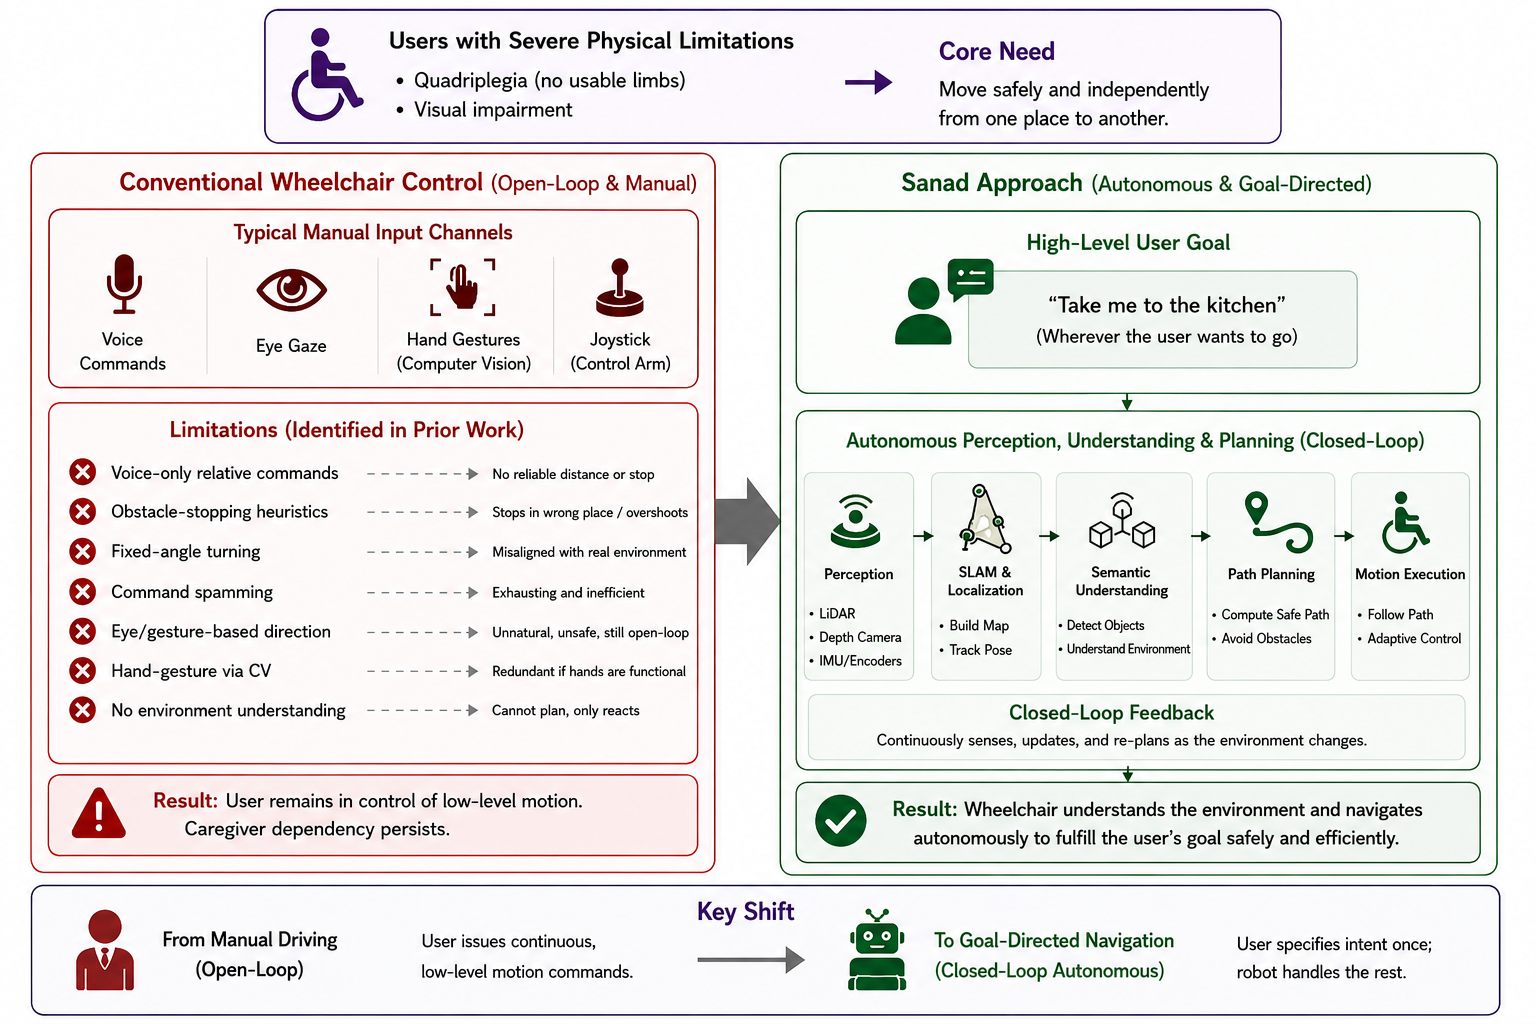
\includegraphics[width=0.75\textwidth]{figures/ch03/problem_statement_comparison.png}
    \caption{Manual/open-loop control (traditional and prior graduation projects) vs. Sanad's autonomous, goal-directed control model.}
    \label{fig:problem_statement_comparison}
\end{figure}

\section{Statistics \& Numbers}

The scale of the problem Sanad addresses is significant both globally and locally:

\begin{itemize}
    \item The World Health Organization estimates that approximately \textbf{80 million people worldwide} (roughly 1\% of the global population) require a wheelchair for mobility, and that this number continues to grow due to population aging, spinal cord injuries, and chronic health conditions~\cite{who2023wheelchair}.
    \item In low- and middle-income countries, the gap between need and access is especially severe: an estimated \textbf{60--75\% of people who need a wheelchair do not have access to one} appropriate for their condition, due to cost, import duties, and limited distribution infrastructure~\cite{ameco2025wheelchairmarket, ncbi2024wheelchairprovision}.
    \item In \textbf{Egypt}, estimates of the number of people living with disabilities vary widely depending on the source and methodology, ranging from around \textbf{2.4 million} (2006 national census, 1.8\% of the population) to \textbf{12--15 million} (UNDP / National Academy for Information Technology for Persons with Disabilities estimates, roughly 8.8--15\% of the population)~\cite{wikipedia2023disabilityegypt, egyptianstreets2024disability, naid2026about}. A 2018 AUC report indicates that around \textbf{15\% of Egyptians with disabilities} have a physical impairment, a subset of which corresponds to wheelchair-dependent individuals.
    \item Among wheelchair users specifically, a meaningful fraction have \textbf{quadriplegia or equivalent total-mobility loss} (e.g., due to spinal cord injury, ALS, cerebral palsy, or stroke), and a smaller but non-trivial fraction are additionally visually impaired --- both groups fall entirely outside what a manual joystick-controlled chair can serve.
    \item Recent published research on ROS-based voice-controlled smart wheelchairs reports mean localization errors below 10~cm and goal-completion rates around 94\% using LiDAR SLAM and AMCL localization~\cite{benayed2026voicecontrolled} --- figures that confirm the technical feasibility of the autonomous, SLAM-based approach Sanad adopts, and serve as a useful benchmark for Sanad's own evaluation.
\end{itemize}


\section{Gap in the Market}

Sanad's positioning becomes clear once the landscape is compared layer by layer: commercial products, international research, and local (Egyptian) graduation projects. Table~\ref{table:gap_summary} summarizes what each layer already offers and what it is still missing.
\begin{table}[H]
\centering
\caption{Summary of the market/research gap across commercial, international, and local layers.}
\label{tab:market_gap}

\begin{tabular}{|>{\raggedright\arraybackslash}p{2.8cm}|
                >{\raggedright\arraybackslash}p{5.4cm}|
                >{\raggedright\arraybackslash}p{5.4cm}|}
\hline
\textbf{Layer} & \textbf{What exists} & \textbf{What's missing} \\
\hline

\textbf{Commercial products}
\begin{itemize}[leftmargin=*,nosep]
    \item WHILL
    \item LUCI
    \item DROVE
\end{itemize}
&
\begin{itemize}[leftmargin=*,nosep]
    \item Proven autonomous driving and safety systems.
    \item Successfully deployed at scale (e.g., airports, retrofit kits).
\end{itemize}
&
\begin{itemize}[leftmargin=*,nosep]
    \item No support for users with zero limb or vision capability.
    \item Autonomy is limited to fixed, pre-mapped destinations.
\end{itemize}
\\
\hline

\textbf{International research}
\begin{itemize}[leftmargin=*,nosep]
    \item VAHM
    \item WAD
    \item CoNav Chair
    \item Benayed \& Masmoudi (2026)
\end{itemize}
&
\begin{itemize}[leftmargin=*,nosep]
    \item SLAM-based navigation.
    \item Voice control.
    \item Multimodal input techniques demonstrated individually.
\end{itemize}
&
\begin{itemize}[leftmargin=*,nosep]
    \item No single system integrates:
    \begin{itemize}[leftmargin=*,nosep]
        \item Full autonomous navigation.
        \item Eye tracking.
        \item Smart-home control.
        \item Remote communication.
    \end{itemize}
\end{itemize}
\\
\hline

\textbf{Egyptian graduation projects}
\begin{itemize}[leftmargin=*,nosep]
    \item ITIDA projects~\cite{itida2021gradprojects}
\end{itemize}
&
\begin{itemize}[leftmargin=*,nosep]
    \item Voice-controlled wheelchair prototypes.
    \item EEG-controlled wheelchair prototypes.
    \item Eye-movement-controlled wheelchair prototypes.
\end{itemize}
&
\begin{itemize}[leftmargin=*,nosep]
    \item All remain manual/open-loop.
    \item None perform autonomous mapping or path planning.
\end{itemize}
\\
\hline

\end{tabular}
\end{table}

The pattern repeats at every layer: autonomous navigation and fully accessible, no-limb/no-vision control have each been demonstrated separately, but never combined --- together with smart-home integration and independent caregiver communication --- into a single home-use platform. This is precisely the combination Sanad is designed to deliver, and it is the basis for the ``What is Sanad?'' description in the next section.

\section{What is Sanad?}

Sanad is an \textbf{autonomous, ROS~2-based smart wheelchair} designed for users with severe mobility impairments, including quadriplegia and visual impairment. Unlike traditional powered wheelchairs, Sanad builds a live map of its environment using LiDAR-based SLAM and localizes itself within that map using AMCL, allowing it to plan and execute paths to a destination on its own once the user specifies a high-level goal, instead of requiring continuous manual steering.

The system is organized around several integrated capabilities:

\begin{itemize}
    \item \textbf{Autonomous indoor navigation}: SLAM Toolbox for mapping, AMCL for localization, and Nav2 for path planning and obstacle avoidance, so that a command such as ``go to the kitchen'' is executed end-to-end without further input from the user.
    \item \textbf{Multi-modal, accessibility-first input}: the primary interaction channel is natural-language voice control (in Arabic), interpreted through an LLM-based intent router. For users who retain some hand mobility, a touch-screen interface is available as a faster alternative. For users who cannot speak or use their hands at all, an \textbf{eye-tracking} interface allows navigation and control purely through gaze. A camera-based \textbf{head-tilt/IMU} controller additionally allows fine, low-speed maneuvering once the chair has reached a room.
    \item \textbf{Vision-Language Model (VLM) assisted navigation}: rather than requiring a pre-labeled destination, a user can describe an object or place in natural language (e.g., ``take me next to the fridge''), and a depth camera combined with a VLM locates the target within the observed scene and provides a navigation goal to the planner.
    \item \textbf{Smart-home control}: integration with home appliances (lighting, television, air conditioning, etc.) via IR blasters and network-connected devices, so the same voice/eye/touch interface that controls mobility also controls the user's immediate environment.
    \item \textbf{Remote communication}: a Telegram-based module allows the user to dictate and autonomously send messages to family members or caregivers without assistance, restoring a channel of independent communication.
    \item \textbf{Natural-language text-to-speech feedback}: Gemini-based TTS provides spoken confirmations and responses, closing the interaction loop for users who cannot read a screen.
\end{itemize}

\begin{figure}[H]
    \centering
    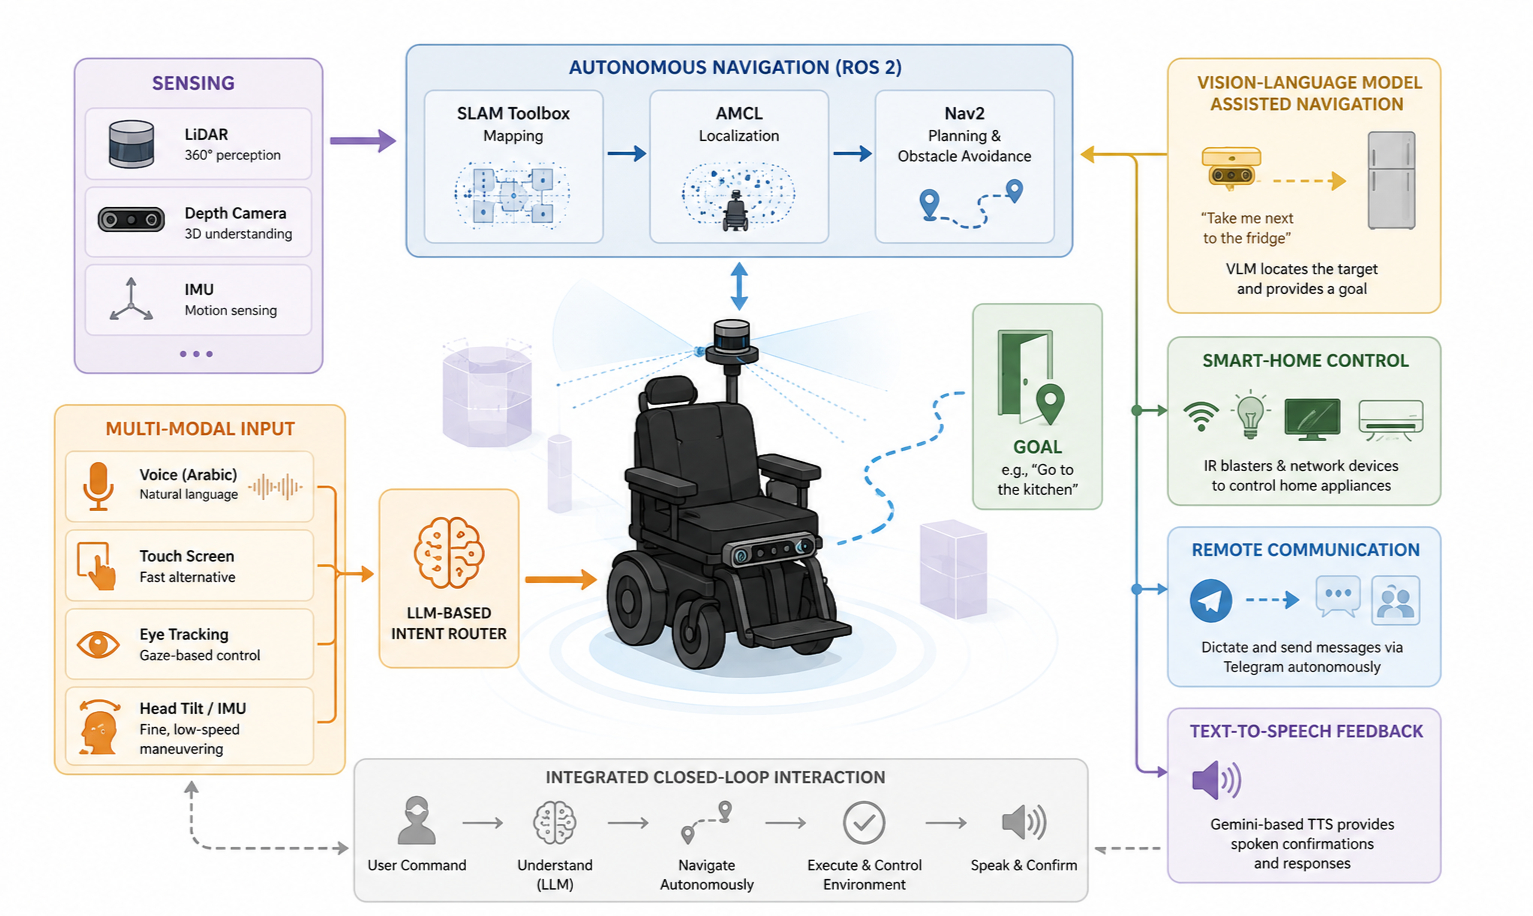
\includegraphics[width=0.8\textwidth]{figures/ch03/sanad_system_overview.png}
    \caption{High-level overview of the Sanad system: sensing, autonomous navigation, and multi-modal control/communication modules.}
    \label{fig:sanad_overview}
\end{figure}

\section{Target Users}

Sanad is designed primarily for:

\begin{itemize}
    \item \textbf{Individuals with quadriplegia} or equivalent total/near-total loss of limb mobility (e.g., due to spinal cord injury, advanced ALS, severe cerebral palsy, or stroke), who cannot operate a joystick or manual control arm.
    \item \textbf{Users with combined mobility and visual impairment}, who cannot rely on sight to judge distances, doorways, or obstacles even if an alternative manual input were available to them.
    \item \textbf{Users with limited or no speech}, who can still interact with Sanad through the eye-tracking interface.
    \item Secondarily, \textbf{users with partial hand mobility} who benefit from the touch-screen interface as a faster alternative to full manual driving, and their \textbf{caregivers}, who benefit from reduced supervision requirements and from the smart-home and communication features.
\end{itemize}


\begin{table}[H]
\centering
\caption{Representative user profiles considered during the requirements analysis.}
\label{tab:user_personas}
\renewcommand{\arraystretch}{1.4}

\begin{tabularx}{\textwidth}{|>{\centering\arraybackslash}p{1.8cm}|
                                >{\raggedright\arraybackslash}p{2.8cm}|
                                >{\raggedright\arraybackslash}X|
                                >{\raggedright\arraybackslash}X|
                                >{\raggedright\arraybackslash}X|}
\hline
\textbf{User Profile} &
\textbf{Disability} &
\textbf{Control Method} &
\textbf{Primary Need} &
\textbf{Relevant Sanad Features} \\
\hline

Profile 1 &
Quadriplegia &
Voice commands or IMU-based head control &
Independent mobility without hand movement &
Autonomous navigation, obstacle avoidance, voice interface, and head-motion control. \\
\hline

Profile 2 &
Quadriplegia with visual impairment &
Voice commands &
Safe navigation without visual feedback &
Autonomous navigation, voice interface, obstacle avoidance, and audio feedback. \\
\hline

Profile 3 &
Complete paralysis with speech impairment &
Eye tracking &
Hands-free and speech-free wheelchair control &
Eye-tracking interface, autonomous navigation, and obstacle avoidance. \\
\hline

Profile 4 &
Lower-limb disability &
Touchscreen interface &
Comfortable navigation with minimal manual driving &
Touchscreen destination selection, autonomous navigation, and smart home integration. \\
\hline

\end{tabularx}
\end{table}

\noindent\textbf{Note:} Profile~4 is capable of operating a conventional powered wheelchair using manual controls. However, this user chooses \textit{Sanad} to benefit from autonomous navigation, easier movement within the home environment, and reduced physical effort compared to continuous manual control.

\section{Summary and Transition}
This chapter has outlined the design space and objectives of the Sanad assistive wheelchair, framing it as an autonomous solution to manual-control limitations. The next chapter, Chapter 2 (Literature Review and Market Analysis), builds upon this context by analyzing existing academic research and benchmarking commercial offerings to locate Sanad within the state of the art.

\chapterseparator{Chapter 2}
\setcounter{chapter}{2}
\chapter*{Chapter (2): Literature Review and \\ Market Analysis}
\addcontentsline{toc}{chapter}{Chapter (2): Literature Review and Market Analysis}
\setcounter{section}{0}

\section{Chapter Preview}
This chapter contextualizes the Sanad project within the existing landscape of assistive mobility technologies. It reviews alternative-input control and autonomous navigation academic research, details the comparative features and limitations of commercial products (such as WHILL, LUCI, and DROVE), and establishes Sanad's unique differentiators.

\section{Existing Smart Wheelchair Research}

Research on smart and autonomous wheelchairs has evolved along two largely separate tracks, which Sanad aims to merge.

\textbf{Alternative-input control research.} Early and influential systems such as \textbf{VAHM} (Voice Activated Head Motion) combined speech recognition with head-movement sensing to give users with limited upper-limb mobility a way to drive a wheelchair without a joystick~\cite{benayed2026voicecontrolled}. This line of work established that non-joystick inputs are viable, but --- consistent with the analysis in Section~1.1 --- most of these systems remained manual/open-loop: the user directly drives the chair through the alternative input rather than specifying a destination for the robot to reach on its own.

\textbf{Autonomous navigation research.} A parallel track, exemplified by systems such as \textbf{WAD} (Wheelchair Autonomous Driving), focused on ROS-based perception and mapping to enable real-time obstacle avoidance and autonomous driving, independent of the specific input modality used to issue commands~\cite{benayed2026voicecontrolled}. More recent work has pushed this further: the \textbf{CoNav Chair} (2025)~\cite{conavchair2025arxiv} introduces shared control built on ROS and 3D SLAM to balance user input with safety constraints, and Cui et al. (2024)~\cite{cui2024intelligent} combine multimodal interaction (voice, gestures, head posture) with LiDAR/SLAM-based autonomous navigation, reporting high positioning accuracy. A 2026 study by Benayed and Masmoudi~\cite{benayed2026voicecontrolled} presents a fully integrated voice-controlled smart wheelchair built on 2D LiDAR SLAM (GMapping) and AMCL localization within a ROS Navigation stack, reporting a mean localization error below 10~cm, a 94\% goal-completion rate, and an end-to-end voice-to-motion latency of 0.8~s, which is a useful reference point for Sanad's own navigation stack (also SLAM Toolbox/AMCL/Nav2-based).

A broader literature survey on smart wheelchair systems highlights additional recurring themes relevant to Sanad: the use of biosignals and head-gesture sensing for motion control, the application of deep learning to control-signal interpretation, and --- notably --- persistent practical limitations such as restriction to indoor use and the need for user training before reliable operation~\cite{arxiv2023smartwheelchairreview}. These limitations mirror exactly the target environment Sanad is designed for (structured indoor spaces such as homes) and motivate Sanad's emphasis on a low-training-burden interface (natural-language voice, eye gaze) rather than a system requiring extensive calibration or practice.

What is comparatively rare in the literature is the \textbf{combination} of (1) fully autonomous, map-based navigation, (2) genuinely accessibility-first multi-modal input that includes eye tracking for users with no reliable speech or limb control, and (3) integrated smart-home and remote-communication capabilities, all within a single platform. Most published systems optimize one of these axes in isolation. This combination is the primary contribution and differentiator of Sanad relative to the reviewed literature.

\section{Commercial Products Comparison}

Beyond generic joystick-driven wheelchairs, a small number of companies and research labs have shipped genuinely \emph{autonomous} wheelchair products. The most relevant ones the team benchmarked against are:

\begin{itemize}
    \item \textbf{WHILL} (incl. the WHILL/Panasonic ``WHILL NEXT'' collaboration): a commercially deployed autonomous wheelchair used mainly as an airport/venue mobility service (Miami International, LAX, Sea-Tac, Schiphol). It uses LiDAR and cameras for obstacle avoidance, and lets a rider select a destination on a touchscreen or summon the chair via a smartphone app; some versions support voice-stated destinations~\cite{whill2025product, whill2026autonomousservice, thedrive2019selfdriving, runwaygirl2024whill, fte2024schiphol}. Critically, WHILL's autonomy is \textbf{geofenced and route-based} (pre-mapped venue routes, predefined destinations) rather than general-purpose indoor SLAM, and it explicitly requires the rider to be able to get in and out of the chair and walk short distances unassisted --- i.e., it targets reduced-mobility travelers, not quadriplegic users~\cite{runwaygirl2024whill, djph2026autonomousdeployment}.
    \item \textbf{LUCI}: a retrofit ``smart module'' that bolts onto an existing power wheelchair and adds collision/tip-over safety enforcement using stereo vision, radar, and ultrasonic sensors. LUCI deliberately focuses on \textbf{safety supervision of manual joystick driving} rather than destination-based autonomy --- it does not navigate the user to a goal on its own~\cite{sunrisemedical2022luci, djph2026autonomousdeployment}. It still requires the user to actively drive with a joystick, so it does not help quadriplegic or visually impaired users.
    \item \textbf{DROVE}: a home-oriented autonomous module allowing selection of pre-defined destinations to traverse corridors/doorways with reduced manual joystick input, but --- like WHILL --- limited to a fixed set of pre-configured destinations rather than open-ended, freely described goals~\cite{djph2026autonomousdeployment}.
\end{itemize}

None of these commercial systems combine full indoor SLAM-based autonomy with a control interface that requires \emph{no} residual limb or visual capability (i.e., voice + eye tracking together), and none integrate smart-home control or independent caregiver communication. The two tables below make this comparison explicit: Table~\ref{table:grad_projects_comparison} compares Sanad against the prior graduation projects reviewed by the team, and Table~\ref{table:commercial_comparison} compares Sanad against the three commercial systems described above.

\begin{table}[H]
\centering
\caption{Comparison between Sanad and prior graduation projects reviewed by the team.}
\begin{tabular}{|p{4cm}|p{5.7cm}|p{5.7cm}|}
\hline
\textbf{Feature} & \textbf{Prior graduation projects} & \textbf{Sanad} \\
\hline
Control paradigm & Manual, open-loop (voice-as-driving, gaze-as-driving, or gesture-as-driving) & Autonomous, goal-directed (SLAM/Nav2 path planning) \\
\hline
Environment mapping & None; reacts only to raw user commands or basic obstacle sensors & Builds/maintains a live SLAM map of any indoor environment \\
\hline
Destination specification & Step-by-step low-level motion commands (distance, direction, angle), re-issued repeatedly & Free-form natural-language goal (``go to the kitchen'', VLM-located objects) \\
\hline
Usable by quadriplegic users (no limb control) & Largely unsupported; most alternative-input systems still assume some residual physical control & Yes --- voice, eye tracking, IMU head-tilt \\
\hline
Usable by visually impaired users & Not addressed & Yes --- voice-driven autonomous navigation removes the need to see the environment \\
\hline
Smart-home control & Not included & Integrated (IR blasters, connected devices) \\
\hline
Remote communication (e.g., messaging caregivers) & Not included & Integrated (autonomous Telegram messaging) \\
\hline
Deployment stage & Prototype only, not commercialized & Prototype, target: low-cost, locally buildable \\
\hline
\end{tabular}
\label{table:grad_projects_comparison}
\end{table}

\begin{table}[H]
\centering
\caption{Comparison between Sanad and commercial autonomous/semi-autonomous wheelchair products (WHILL, LUCI, DROVE).}
\begin{tabular}{|p{2.9cm}|p{2.9cm}|p{2.9cm}|p{2.9cm}|p{2.9cm}|}
\hline
\textbf{Feature} & \textbf{WHILL} & \textbf{LUCI} & \textbf{DROVE} & \textbf{Sanad} \\
\hline
Control paradigm & Route/geofenced autonomy on pre-mapped venue paths & Manual joystick driving with AI safety supervision only & Route autonomy over a fixed set of pre-defined home destinations & Autonomous, goal-directed (SLAM/Nav2 path planning) \\
\hline
Environment mapping & Pre-mapped fixed venue routes, no live SLAM & None; live sensor fusion (stereo vision, radar, ultrasonic) for collision avoidance only & Pre-configured fixed destinations, no general SLAM & Builds/maintains a live SLAM map of any indoor environment \\
\hline
Destination specification & Touchscreen/app selection from a fixed destination list; some voice-stated destinations & N/A --- user drives manually via joystick & Selection from a fixed, pre-defined destination list & Free-form natural-language goal, incl.\ VLM-located objects \\
\hline
Usable by quadriplegic users (no limb control) & No --- requires touchscreen/app use and unassisted transfer in/out of the chair & No --- requires active joystick driving & No --- requires touchscreen/app selection & Yes --- voice, eye tracking, IMU head-tilt \\
\hline
Usable by visually impaired users & Not addressed; touchscreen-centric interaction & Not addressed & Not addressed; touchscreen-centric interaction & Yes --- voice-driven autonomous navigation \\
\hline
Deployment context & Public venues (airports) as a shared fleet service & Retrofit module for an existing personal power wheelchair & Personal, home/indoor use & Personal, home/indoor use \\
\hline
Smart-home control & Not included & Not included & Not included & Integrated (IR blasters, connected devices) \\
\hline
Remote communication & Not included & Not included & Not included & Integrated (autonomous Telegram messaging) \\
\hline
Cost/availability & Commercial, \$4,000+ per unit~\cite{harvard2020whillcase} or B2B fleet service, not sold for personal home use & Commercial retrofit add-on for existing power wheelchairs & Not broadly commercially available (research/early product stage) & Student graduation-project platform (target: low-cost, locally buildable) \\
\hline
\end{tabular}
\label{table:commercial_comparison}
\end{table}

\section{Summary and Transition}
This chapter has benchmarked Sanad against existing academic literature and commercial smart wheelchairs, highlighting the gap in unified, accessible, and autonomous systems. The next chapter, Chapter 3 (System Architecture), details the high-level physical and logical design that addresses these gaps.




\chapterseparator{Chapter 3}
\setcounter{chapter}{3}
\chapter*{Chapter (3): System Architecture}
\addcontentsline{toc}{chapter}{Chapter (3): System Architecture}
\setcounter{section}{0}

\section{Chapter Preview}
This chapter presents the architectural blueprint of the Sanad system. It introduces the high-level hardware-software component layout, details the layered model that decouples core robotics from presentation interfaces, describes the ROS 2 middleware, and traces the lifecycle of a command flow.

\section{System Overview}
\label{sec:arch_overview}

Chapters~1 and~2 established \emph{why} Sanad exists and \emph{what} it must do: replace manual, open-loop wheelchair control with autonomous, goal-directed navigation, driven by an accessibility-first set of input modalities and supported by smart-home and communication features. This chapter answers the next question --- \emph{how the system is put together} --- before Chapters~4 through~11 descend into the implementation of each individual subsystem.

Figure~\ref{fig:system_overview_full} shows every major hardware and software component of Sanad on a single page, deliberately stripped of internal detail. Its only purpose is to give the reader a mental map of the system before the rest of this chapter, and the rest of this book, zooms into each block in turn.

\begin{figure}[H]
\centering
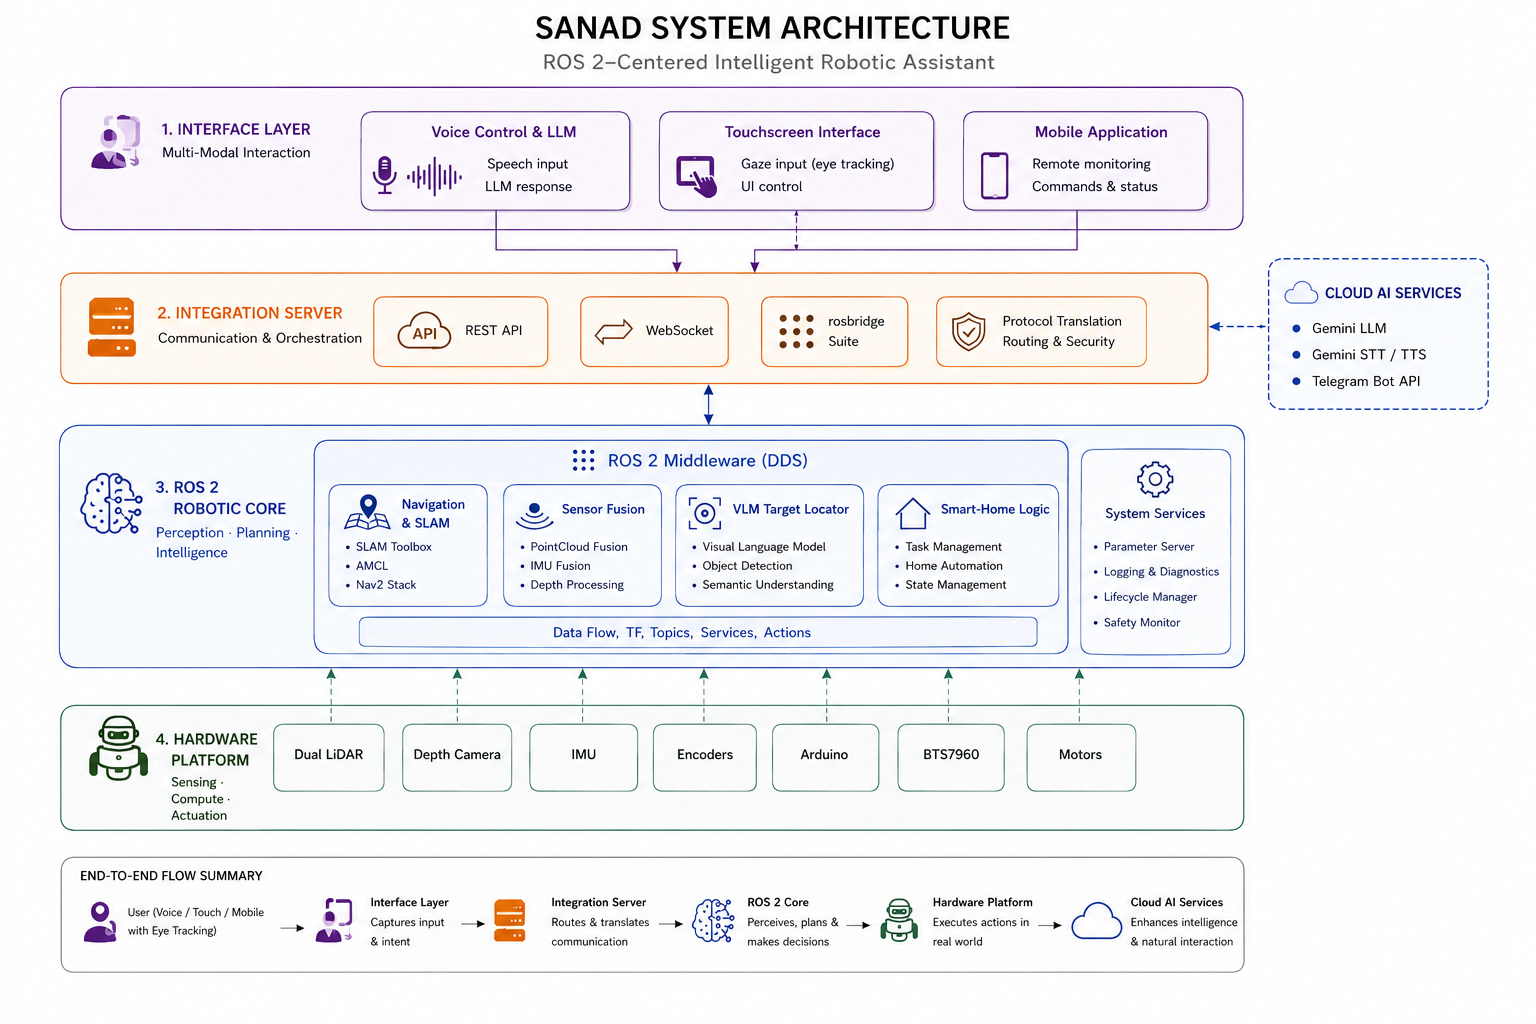
\includegraphics[width=\textwidth]{figures/ch03/system_archtict.png}
\caption{High-level overview of the Sanad system, showing all major hardware and software components organized around the central SANAD Integration Server. Each block is expanded in the corresponding subsystem chapter.}
\label{fig:system_overview_full}
\end{figure}

At a glance, Sanad is composed of five groups of components:

\begin{itemize}
    \item \textbf{Interface Layer} --- five parallel input channels (voice, touchscreen, eye tracking, mobile app, IMU head-tilt) through which a user or caregiver expresses intent, covered in Chapters~5, 7, 8, and~9.
    \item \textbf{Integration Server} --- a single Node.js service that translates between web-facing protocols (REST, WebSocket) and the robot's internal ROS~2 messaging, detailed in Chapter~6.
    \item \textbf{Robotic Core (ROS~2)} --- the autonomous decision-making and motion layer: navigation and SLAM, the voice/LLM intent router, VLM-based target location, and smart-home/communication logic, covered in Chapters~4 and~5.
    \item \textbf{Hardware Platform} --- the physical sensor suite and actuation subsystem that let the robot perceive and move through the world, covered in Chapter~10.
    \item \textbf{Cloud AI Services} --- external, network-dependent services (Gemini LLM, Gemini speech synthesis/recognition, the Telegram Bot API) that the Integration Server calls out to, with a local edge fallback discussed in Chapter~5.
\end{itemize}

The remaining sections of this chapter explain the architectural reasoning that ties these groups together, then walk a single command through the full stack end-to-end.

\section{Layered Architectural Model}
\label{sec:arch_layers}

Rather than a monolithic program, Sanad is organized as four stacked layers, each with a single, well-defined responsibility and a narrow interface to its neighbors. This separation --- expanded on for the server specifically in Section~6.1.3 using a SCADA analogy --- is applied here to the system as a whole, so that presentation-layer changes (e.g., a new mobile screen) never require touching motion-control code, and vice versa.

\begin{figure}[H]
\centering
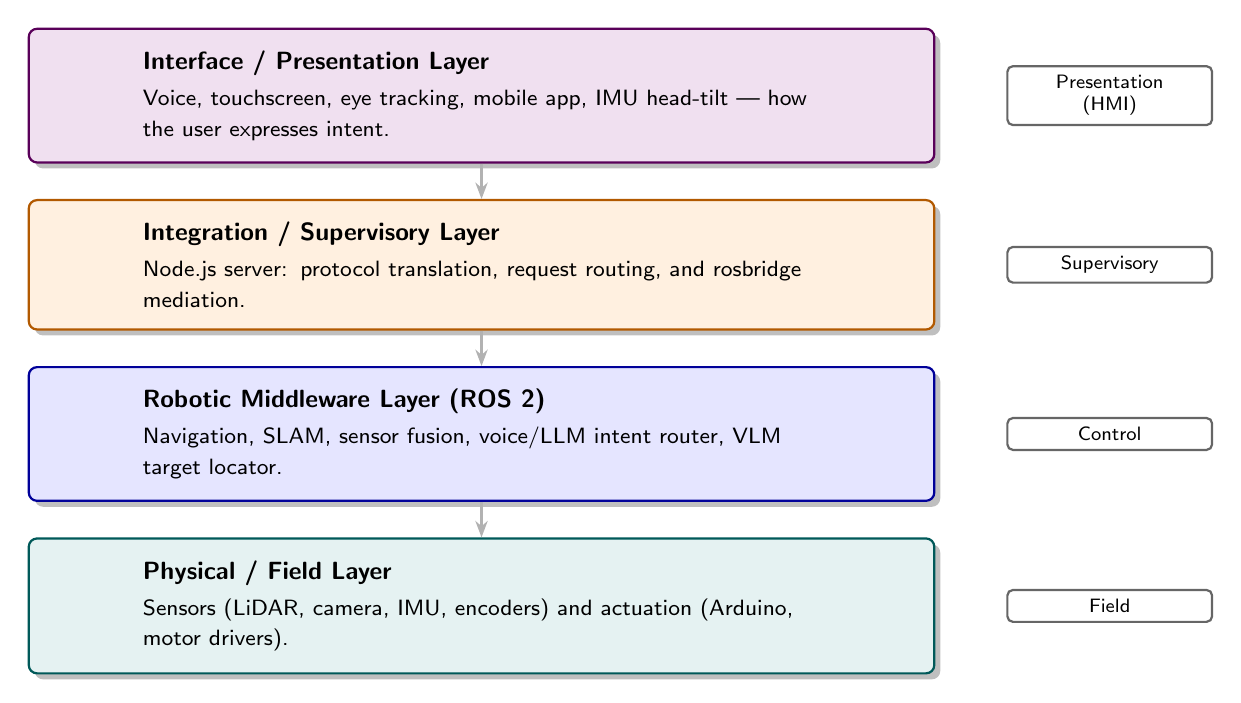
\begin{tikzpicture}[
    font=\sffamily\small,
    layer/.style={draw=black!60, rounded corners=3pt, thick, minimum width=11.5cm,
        minimum height=1.5cm, align=left, text width=8.6cm, inner sep=8pt, drop shadow},
    tag/.style={draw=black!60, fill=white, rounded corners=2pt, font=\sffamily\scriptsize,
        minimum width=2.6cm, align=center, thick}
]

\node[layer, fill=violet!12, draw=violet!70!black] (l1) at (0,4.5)
    {\textbf{Interface / Presentation Layer}\\[2pt]
     \footnotesize Voice, touchscreen, eye tracking, mobile app, IMU head-tilt --- how the user expresses intent.};

\node[layer, fill=orange!12, draw=orange!70!black, below=0.45cm of l1] (l2)
    {\textbf{Integration / Supervisory Layer}\\[2pt]
     \footnotesize Node.js server: protocol translation, request routing, and rosbridge mediation.};

\node[layer, fill=blue!10, draw=blue!60!black, below=0.45cm of l2] (l3)
    {\textbf{Robotic Middleware Layer (ROS~2)}\\[2pt]
     \footnotesize Navigation, SLAM, sensor fusion, voice/LLM intent router, VLM target locator.};

\node[layer, fill=teal!10, draw=teal!70!black, below=0.45cm of l3] (l4)
    {\textbf{Physical / Field Layer}\\[2pt]
     \footnotesize Sensors (LiDAR, camera, IMU, encoders) and actuation (Arduino, motor drivers).};

\node[tag, right=0.9cm of l1] {Presentation\\(HMI)};
\node[tag, right=0.9cm of l2] {Supervisory};
\node[tag, right=0.9cm of l3] {Control};
\node[tag, right=0.9cm of l4] {Field};

\draw[-{Stealth[scale=0.9]}, thick, draw=gray!60] (l1.south) -- (l2.north);
\draw[-{Stealth[scale=0.9]}, thick, draw=gray!60] (l2.south) -- (l3.north);
\draw[-{Stealth[scale=0.9]}, thick, draw=gray!60] (l3.south) -- (l4.north);

\end{tikzpicture}
\caption{The four-layer architectural model of Sanad, adapted from a SCADA-style stratification of responsibilities (see also Section~6.1.3).}
\label{fig:layered_architecture}
\end{figure}

Two design rules follow directly from this layering. First, \textbf{no layer may skip its neighbor}: a touchscreen button never talks to a ROS~2 node directly, and a navigation node never renders UI --- every cross-layer interaction is mediated by the Integration Server. Second, \textbf{ROS~2 is treated as the boundary of real-time responsibility}: everything at or below the Robotic Middleware Layer must tolerate hard timing constraints (control loops, sensor rates), while everything above it may be arbitrarily delayed by network conditions without endangering the robot, since motion always degrades safely (Chapter~4 covers the relevant safety behaviors).

\section{Hardware Platform}
\label{sec:arch_hardware}

At the base of the stack sits the physical wheelchair platform: a retrofitted manual chair carrying a dual 2D LiDAR array, a depth camera, a chassis IMU, quadrature wheel encoders, and a differential-drive actuation system built around BTS7960 motor drivers and an Arduino running a closed-loop PID velocity controller. An onboard computer runs the ROS~2 graph and communicates with the Arduino over a serial link using the \texttt{SanadInterface} protocol. This chapter treats the hardware platform as a single opaque block (the \textit{Sensor Suite} and \textit{Actuation Subsystem} in Figure~\ref{fig:system_overview_full}); the physical modifications, mechanical calculations, PID tuning, and circuit design are covered in full in Chapter~10.

\section{Robotic Middleware: The ROS~2 Core}
\label{sec:arch_ros2core}

The Robotic Middleware Layer is where perception turns into motion. It is implemented entirely as a graph of ROS~2 nodes communicating over topics, services, and actions, which gives Sanad two properties that matter for a safety-relevant assistive device: individual nodes (say, the VLM target locator) can crash or restart without taking down navigation, and the same navigation stack developed and tested in isolation can be driven by any of the five interface channels without modification. Four functional groups make up this core:

\begin{itemize}
    \item \textbf{Navigation \& SLAM} --- sensor preprocessing, EKF-based odometry fusion, SLAM Toolbox/AMCL localization, Nav2 path planning, and trajectory control (Chapter~4).
    \item \textbf{Voice \& LLM Intent Router} --- wake-word detection, speech-to-text, LLM-based intent parsing, and action routing to the correct subsystem (Chapter~5).
    \item \textbf{VLM Target Locator} --- combines the depth camera with a vision-language model to resolve free-text destinations (``next to the fridge'') into navigable coordinates (Chapter~4, Section~4.13).
    \item \textbf{Smart-Home \& Communication} --- IR blaster control and the autonomous Telegram messaging pipeline, exposed to ROS~2 via the same node-based pattern (Chapters~6 and~9).
\end{itemize}

\section{Integration Server \& Client-Server Communication}
\label{sec:arch_server}

Because ROS~2 is optimized for tightly coupled internal communication rather than heterogeneous external clients, Sanad places a single custom Node.js server between the Robotic Middleware Layer and every client above it. The server exposes a stateless REST API for discrete requests, a persistent WebSocket channel for high-frequency motion telemetry, and a dedicated \texttt{rosbridge} integration layer that multiplexes all ROS-facing communication through one supervised connection with automatic teardown-and-rebuild recovery on disconnect. This dual-server, single-bridge design --- along with the feature-module organization of IR control, Telegram integration, and telemetry --- is the subject of Chapter~6 in full.

\section{Multi-Modal Interface Layer}
\label{sec:arch_interfaces}

Sanad deliberately exposes the \emph{same} underlying capabilities (navigation, smart-home control, communication) through five independent front ends, so that a user's degree of residual physical ability determines which channel they use, not which features they can access. Voice control (Chapter~5) is the primary channel, built on a cloud-first, edge-fallback pipeline with Arabic-language support. The touchscreen (Chapter~7) offers a faster alternative for users with partial hand mobility. Eye tracking (Chapter~8) provides gaze-dwell interaction for users with no reliable speech or limb control. The mobile app (Chapter~9) targets caregivers, providing remote monitoring, biometric alerts, and Telegram-based communication. IMU-based head-tilt sensing (Chapter~4, Section~4.12) adds fine, low-speed maneuvering once a room has been reached. All five channels converge on the same Integration Server endpoints described in Section~\ref{sec:arch_server}, so no channel has privileged or duplicated access to robot behavior.

\section{End-to-End Command Flow: A Worked Example}
\label{sec:arch_e2e}

The clearest way to see the layers of Section~\ref{sec:arch_layers} cooperate is to trace one command through all of them. Figure~\ref{fig:e2e_flow} follows the spoken instruction ``take me to the kitchen'' from utterance to physical motion and back to spoken confirmation.

\begin{figure}[H]
\centering
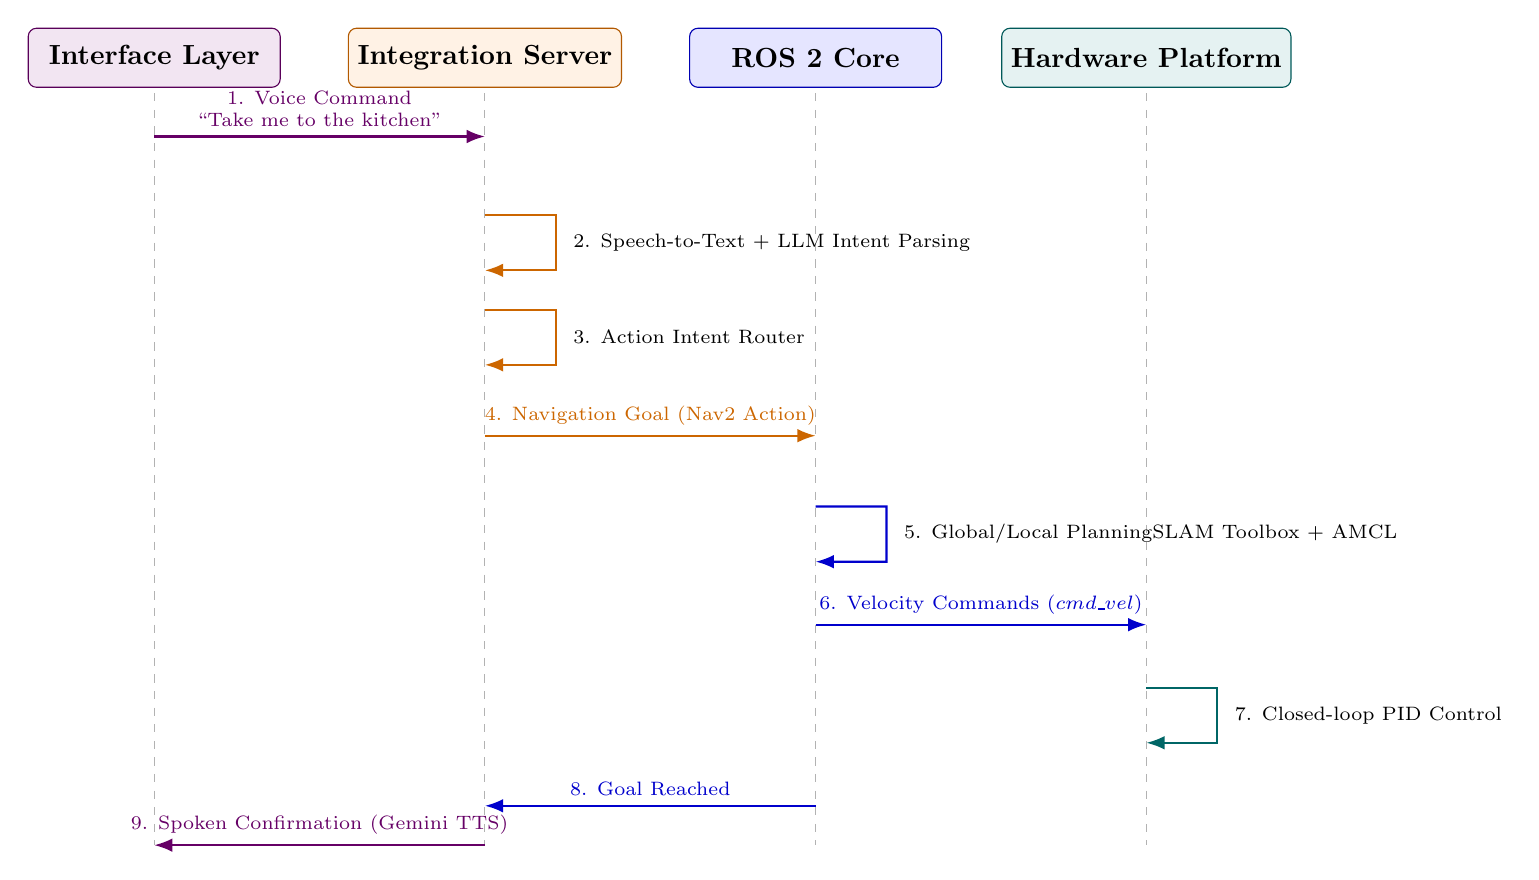
\begin{tikzpicture}[
    >=Latex,
    font=\sffamily\small,
    x=1cm,
    y=1cm
]

%------------------------------------------------
% Participants
%------------------------------------------------
\node[draw=violet!70!black,fill=violet!10,
rounded corners=3pt,
minimum width=3.2cm,
minimum height=0.75cm,
font=\bfseries] (ui) at (0,0)
{Interface Layer};

\node[draw=orange!70!black,fill=orange!10,
rounded corners=3pt,
minimum width=3.2cm,
minimum height=0.75cm,
font=\bfseries] (server) at (4.2,0)
{Integration Server};

\node[draw=blue!70!black,fill=blue!10,
rounded corners=3pt,
minimum width=3.2cm,
minimum height=0.75cm,
font=\bfseries] (ros) at (8.4,0)
{ROS 2 Core};

\node[draw=teal!70!black,fill=teal!10,
rounded corners=3pt,
minimum width=3.2cm,
minimum height=0.75cm,
font=\bfseries] (hw) at (12.6,0)
{Hardware Platform};

%------------------------------------------------
% Lifelines
%------------------------------------------------
\foreach \x in {0,4.2,8.4,12.6}
{
    \draw[dashed,gray!60] (\x,-0.45)--(\x,-10);
}

%------------------------------------------------
% Messages
%------------------------------------------------

%1
\draw[->,thick,violet!80!black]
(0,-1)--(4.2,-1)
node[midway,above,font=\scriptsize,align=center]
{1. Voice Command\\``Take me to the kitchen''};

%2
\draw[->,thick,orange!80!black]
(4.2,-2)--++(0.9,0)
--++(0,-0.7)
--(4.2,-2.7);

\node[anchor=west,font=\scriptsize]
at (5.2,-2.35)
{2. Speech-to-Text + LLM Intent Parsing};

%3
\draw[->,thick,orange!80!black]
(4.2,-3.2)--++(0.9,0)
--++(0,-0.7)
--(4.2,-3.9);

\node[anchor=west,font=\scriptsize]
at (5.2,-3.55)
{3. Action Intent Router};

%4
\draw[->,thick,orange!80!black]
(4.2,-4.8)--(8.4,-4.8)
node[midway,above,font=\scriptsize]
{4. Navigation Goal (Nav2 Action)};

%5
\draw[->,thick,blue!80!black]
(8.4,-5.7)--++(0.9,0)
--++(0,-0.7)
--(8.4,-6.4);

\node[anchor=west,font=\scriptsize]
at (9.4,-6.05)
{5. Global/Local Planning\\SLAM Toolbox + AMCL};

%6
\draw[->,thick,blue!80!black]
(8.4,-7.2)--(12.6,-7.2)
node[midway,above,font=\scriptsize]
{6. Velocity Commands ($cmd\_vel$)};

%7
\draw[->,thick,teal!80!black]
(12.6,-8)--++(0.9,0)
--++(0,-0.7)
--(12.6,-8.7);

\node[anchor=west,font=\scriptsize]
at (13.6,-8.35)
{7. Closed-loop PID Control};

%8
\draw[<-,thick,blue!80!black]
(4.2,-9.5)--(8.4,-9.5)
node[midway,above,font=\scriptsize]
{8. Goal Reached};

%9
\draw[<-,thick,violet!80!black]
(0,-10)--(4.2,-10)
node[midway,above,font=\scriptsize]
{9. Spoken Confirmation (Gemini TTS)};

\end{tikzpicture}

\caption{Sequence diagram illustrating the end-to-end execution of a voice navigation command across the Sanad software architecture.}
\label{fig:e2e_flow}
\end{figure}

Three properties of this flow are worth highlighting because they recur throughout the rest of the book. First, the request crosses the Interface--Integration--Core boundary exactly once in each direction (steps~3 and~7), consistent with the no-skipping rule of Section~\ref{sec:arch_layers}. Second, once the Navigation Goal is accepted in step~4, the robot completes steps~4--6 autonomously and in a hard real-time loop, entirely independent of network conditions --- if the voice channel that issued the command drops, the chair still safely reaches its destination. Third, the same eight-step shape applies almost unchanged to the other four interface channels; only step~1--2 differs (a touchscreen tap or a gaze-dwell selection replaces speech recognition), which is precisely what allows Section~\ref{sec:arch_interfaces}'s five channels to share one navigation implementation.

\section{Chapter Roadmap}
\label{sec:arch_roadmap}

Table~\ref{table:chapter_roadmap} maps each architectural block introduced in this chapter to the chapter that covers its implementation in detail.

\begin{table}[H]
\centering
\caption{Mapping from architectural layer/component to the chapter covering its implementation.}
\begin{tabular}{|p{4.2cm}|p{6.3cm}|p{2.3cm}|}
\hline
\textbf{Layer} & \textbf{Component} & \textbf{Chapter} \\
\hline
\multirow{4}{4.2cm}{Interface Layer} & Voice Control \& LLM & 5 \\
\cline{2-3}
 & Touchscreen Interface & 7 \\
\cline{2-3}
 & Eye Tracking & 8 \\
\cline{2-3}
 & Mobile Application & 9 \\
\hline
Integration Layer & Integration Server & 6 \\
\hline
\multirow{3}{4.2cm}{Robotic Core (ROS~2)} & Navigation \& SLAM, IMU head-tilt, sensor fusion, VLM target locator & 4 \\
\cline{2-3}
 & Voice/LLM intent routing & 5 \\
\cline{2-3}
 & Smart-home \& Telegram modules & 6, 9 \\
\hline
Physical / Field Layer & Hardware \& Implementation & 10 \\
\hline
\end{tabular}
\label{table:chapter_roadmap}
\end{table}

\section{Summary and Transition}
This chapter has established the layered architectural framework that coordinates Sanad's hardware, server middleware, and multi-modal user interfaces. The next chapter, Chapter 4 (Autonomous Navigation), focuses on the robotic core, detailing the sensors, mapping algorithms, and motion control stacks enabling autonomous indoor traversal.

\chapterseparator{Chapter 4}
\setcounter{chapter}{4} 
\chapter*{Chapter (4): Autonomous Navigation}
\addcontentsline{toc}{chapter}{Chapter (4): Autonomous Navigation} 
\setcounter{section}{0}

\section{Chapter Preview}
This chapter details the core autonomous navigation stack of the Sanad assistive robot. It outlines the modular navigation pipeline including sensor data acquisition, filtering, state estimation, SLAM mapping, AMCL localization, global/local path planning, head-gesture control, human-following mode, and semantic Vision-Language Model integration.

The navigation system is designed using a modular pipeline structure, which consists of the following sequential stages:
\begin{figure}[htbp]
\centering
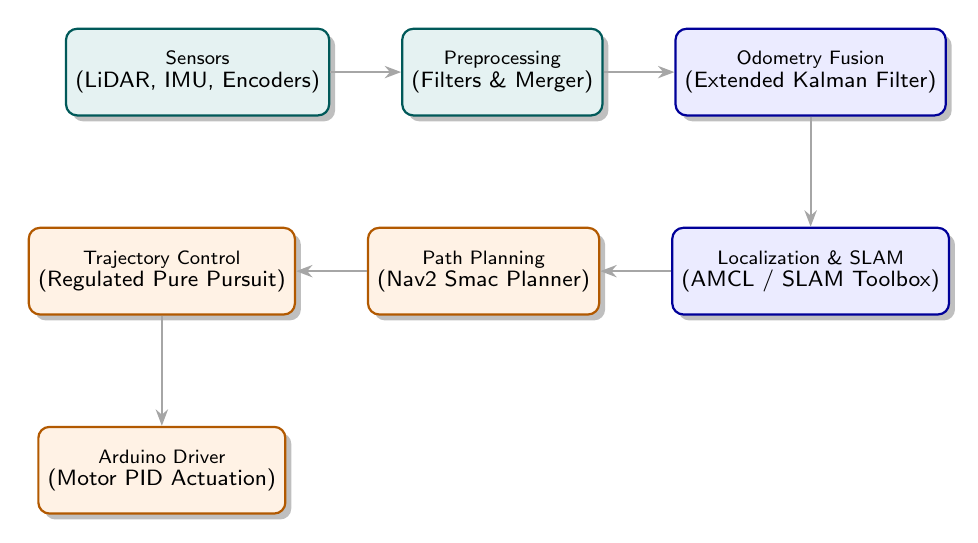
\begin{tikzpicture}[
    node distance=0.9cm,
    font=\sffamily\scriptsize,
    every node/.style={transform shape},
    sense/.style={
        draw=teal!70!black,
        fill=teal!10,
        rectangle,
        rounded corners=4pt,
        align=center,
        minimum width=2.4cm,
        minimum height=1.1cm,
        thick,
        drop shadow
    },
    process/.style={
        draw=blue!60!black,
        fill=blue!8,
        rectangle,
        rounded corners=4pt,
        align=center,
        minimum width=2.4cm,
        minimum height=1.1cm,
        thick,
        drop shadow
    },
    control/.style={
        draw=orange!70!black,
        fill=orange!10,
        rectangle,
        rounded corners=4pt,
        align=center,
        minimum width=2.4cm,
        minimum height=1.1cm,
        thick,
        drop shadow
    },
    arrow/.style={-{Stealth[scale=0.9]}, thick, draw=gray!70}
]

% Nodes - horizontal flow, color-coded by stage
\node[sense] (sensors) {Sensors\\\footnotesize (LiDAR, IMU, Encoders)};
\node[sense, right=of sensors] (preprocess) {Preprocessing\\\footnotesize (Filters \& Merger)};
\node[process, right=of preprocess] (ekf) {Odometry Fusion\\\footnotesize (Extended Kalman Filter)};
\node[process, below=1.4cm of ekf] (loc) {Localization \& SLAM\\\footnotesize (AMCL / SLAM Toolbox)};
\node[control, left=of loc] (plan) {Path Planning\\\footnotesize (Nav2 Smac Planner)};
\node[control, left=of plan] (control_n) {Trajectory Control\\\footnotesize (Regulated Pure Pursuit)};
\node[control, below=1.4cm of control_n] (motor) {Arduino Driver\\\footnotesize (Motor PID Actuation)};

% Arrows - serpentine layout
\draw[arrow] (sensors) -- (preprocess);
\draw[arrow] (preprocess) -- (ekf);
\draw[arrow] (ekf) -- (loc);
\draw[arrow] (loc) -- (plan);
\draw[arrow] (plan) -- (control_n);
\draw[arrow] (control_n) -- (motor);

\end{tikzpicture}
\caption{Flowchart of the Sanad Autonomous Navigation Pipeline.}
\label{fig:navigation_pipeline_flow}
\end{figure}
\begin{enumerate}
    \item \textbf{Data Acquisition}: Captures environment data using dual LiDAR scanners, a depth camera, wheel encoders, and a chassis IMU.
    \item \textbf{Perception \& Preprocessing}: Runs angular filter chains on each LiDAR scan to remove self-obstruction zones, then fuses both filtered scans into a unified 360-degree \texttt{/scan} topic using the \texttt{dual\_laser\_merger} node.
    \item \textbf{State Estimation \& Odometry Fusion}: Implements an Extended Kalman Filter (EKF) to fuse noisy wheel odometry with angular rates and linear accelerations from the IMU, producing a slip-resistant pose estimate.
    \item \textbf{Localization \& Mapping}: Executes SLAM (Simultaneous Localization and Mapping) during the initialization phase to build a grid map, and switches to AMCL (Adaptive Monte Carlo Localization) for real-time tracking during navigation.
    \item \textbf{Global Path Planning}: Computes a collision-free path from the robot's current pose to the target coordinates using a search-based 2D grid planner.
    \item \textbf{Local Trajectory Control}: Computes continuous velocity commands (\texttt{cmd\_vel}) to track the global path, scaling speed based on proximity to obstacles and path curvature.
    \item \textbf{Low-Level Actuation}: The motor controller executes joint commands through a closed-loop PID velocity controller running on the Arduino microcontroller.
\end{enumerate}

Figure~\ref{fig:navigation_pipeline_flow} outlines the data flow through these pipeline stages.



\section{Block 1: Data Acquisition \& Sensors}

The first stage of the navigation pipeline involves acquiring raw environmental and state feedback data from the physical sensor array.

\begin{itemize}
    \item \textbf{Dual LiDAR Scanners (LD06)}: Provide distance measurements in a 2D plane at 10 Hz, mapping obstacles up to 12 meters away.
    \item \textbf{Intel RealSense Depth Camera}: Provides high-resolution RGB-D streams, outputting a 3D point cloud of the forward-facing field.
    \item \textbf{Onboard MPU6050 IMU}: Mounted to the center of the wheelchair chassis, providing 3-axis linear acceleration and angular velocity readings.
    \item \textbf{Wheel Encoders}: Optical incremental encoders attached to both drive motors, measuring wheel rotation counts at high resolution (3436 ticks per revolution).
\end{itemize}

\begin{figure}[H]
    \centering
    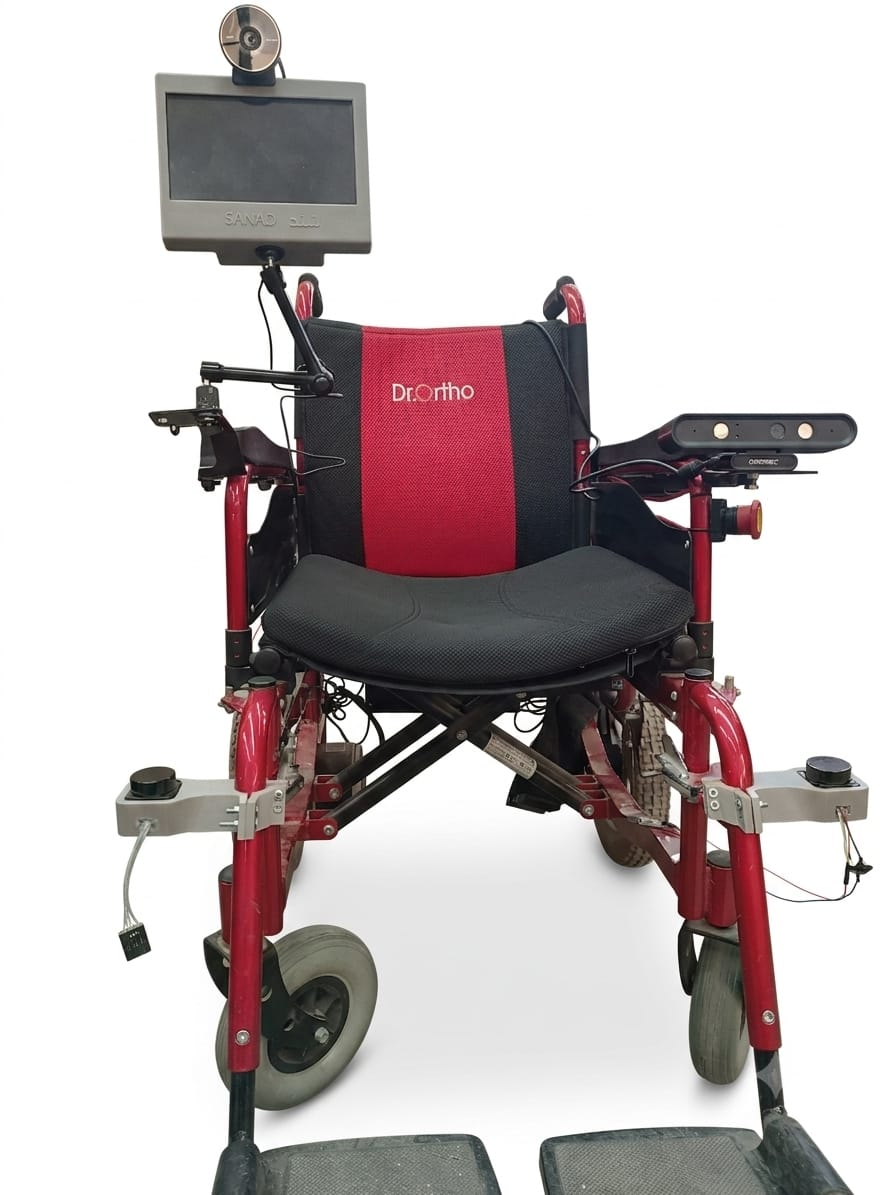
\includegraphics[width=0.8\textwidth]{figures/ch04/full_chair_real.jpeg}
    \caption{Physical sensor mounting layout (LiDARs, Camera, IMU) on the wheelchair.}
    \label{fig:physical_sensors_layout}
\end{figure}

\section{Block 2: Perception \& Preprocessing}

\subsection{Phase 1: LiDAR Scan Cropping}

During testing, a major challenge arose from self-obstruction. Because the LiDARs are mounted directly onto the wheelchair's chassis, the laser beams hit the wheelchair's frame, armrests, wheels, and footrests. This self-obstruction caused the sensors to report static obstacles at zero distance, creating a phantom obstacle in the local costmaps. This constant danger reading triggered safety recovery behaviors, locking the motors.

To solve this, the \texttt{laser\_filters} package was integrated. Specifically, a \texttt{laser\_filters/LaserScanAngularBoundsFilter} plugin was configured to crop out the specific angular sectors where the wheelchair chassis is visible, removing self-obstruction zones.

% --- Single LiDAR: Robot model view + costmap effect ---
\begin{figure}[H]
\centering
\begin{minipage}{0.48\textwidth}
    \centering
    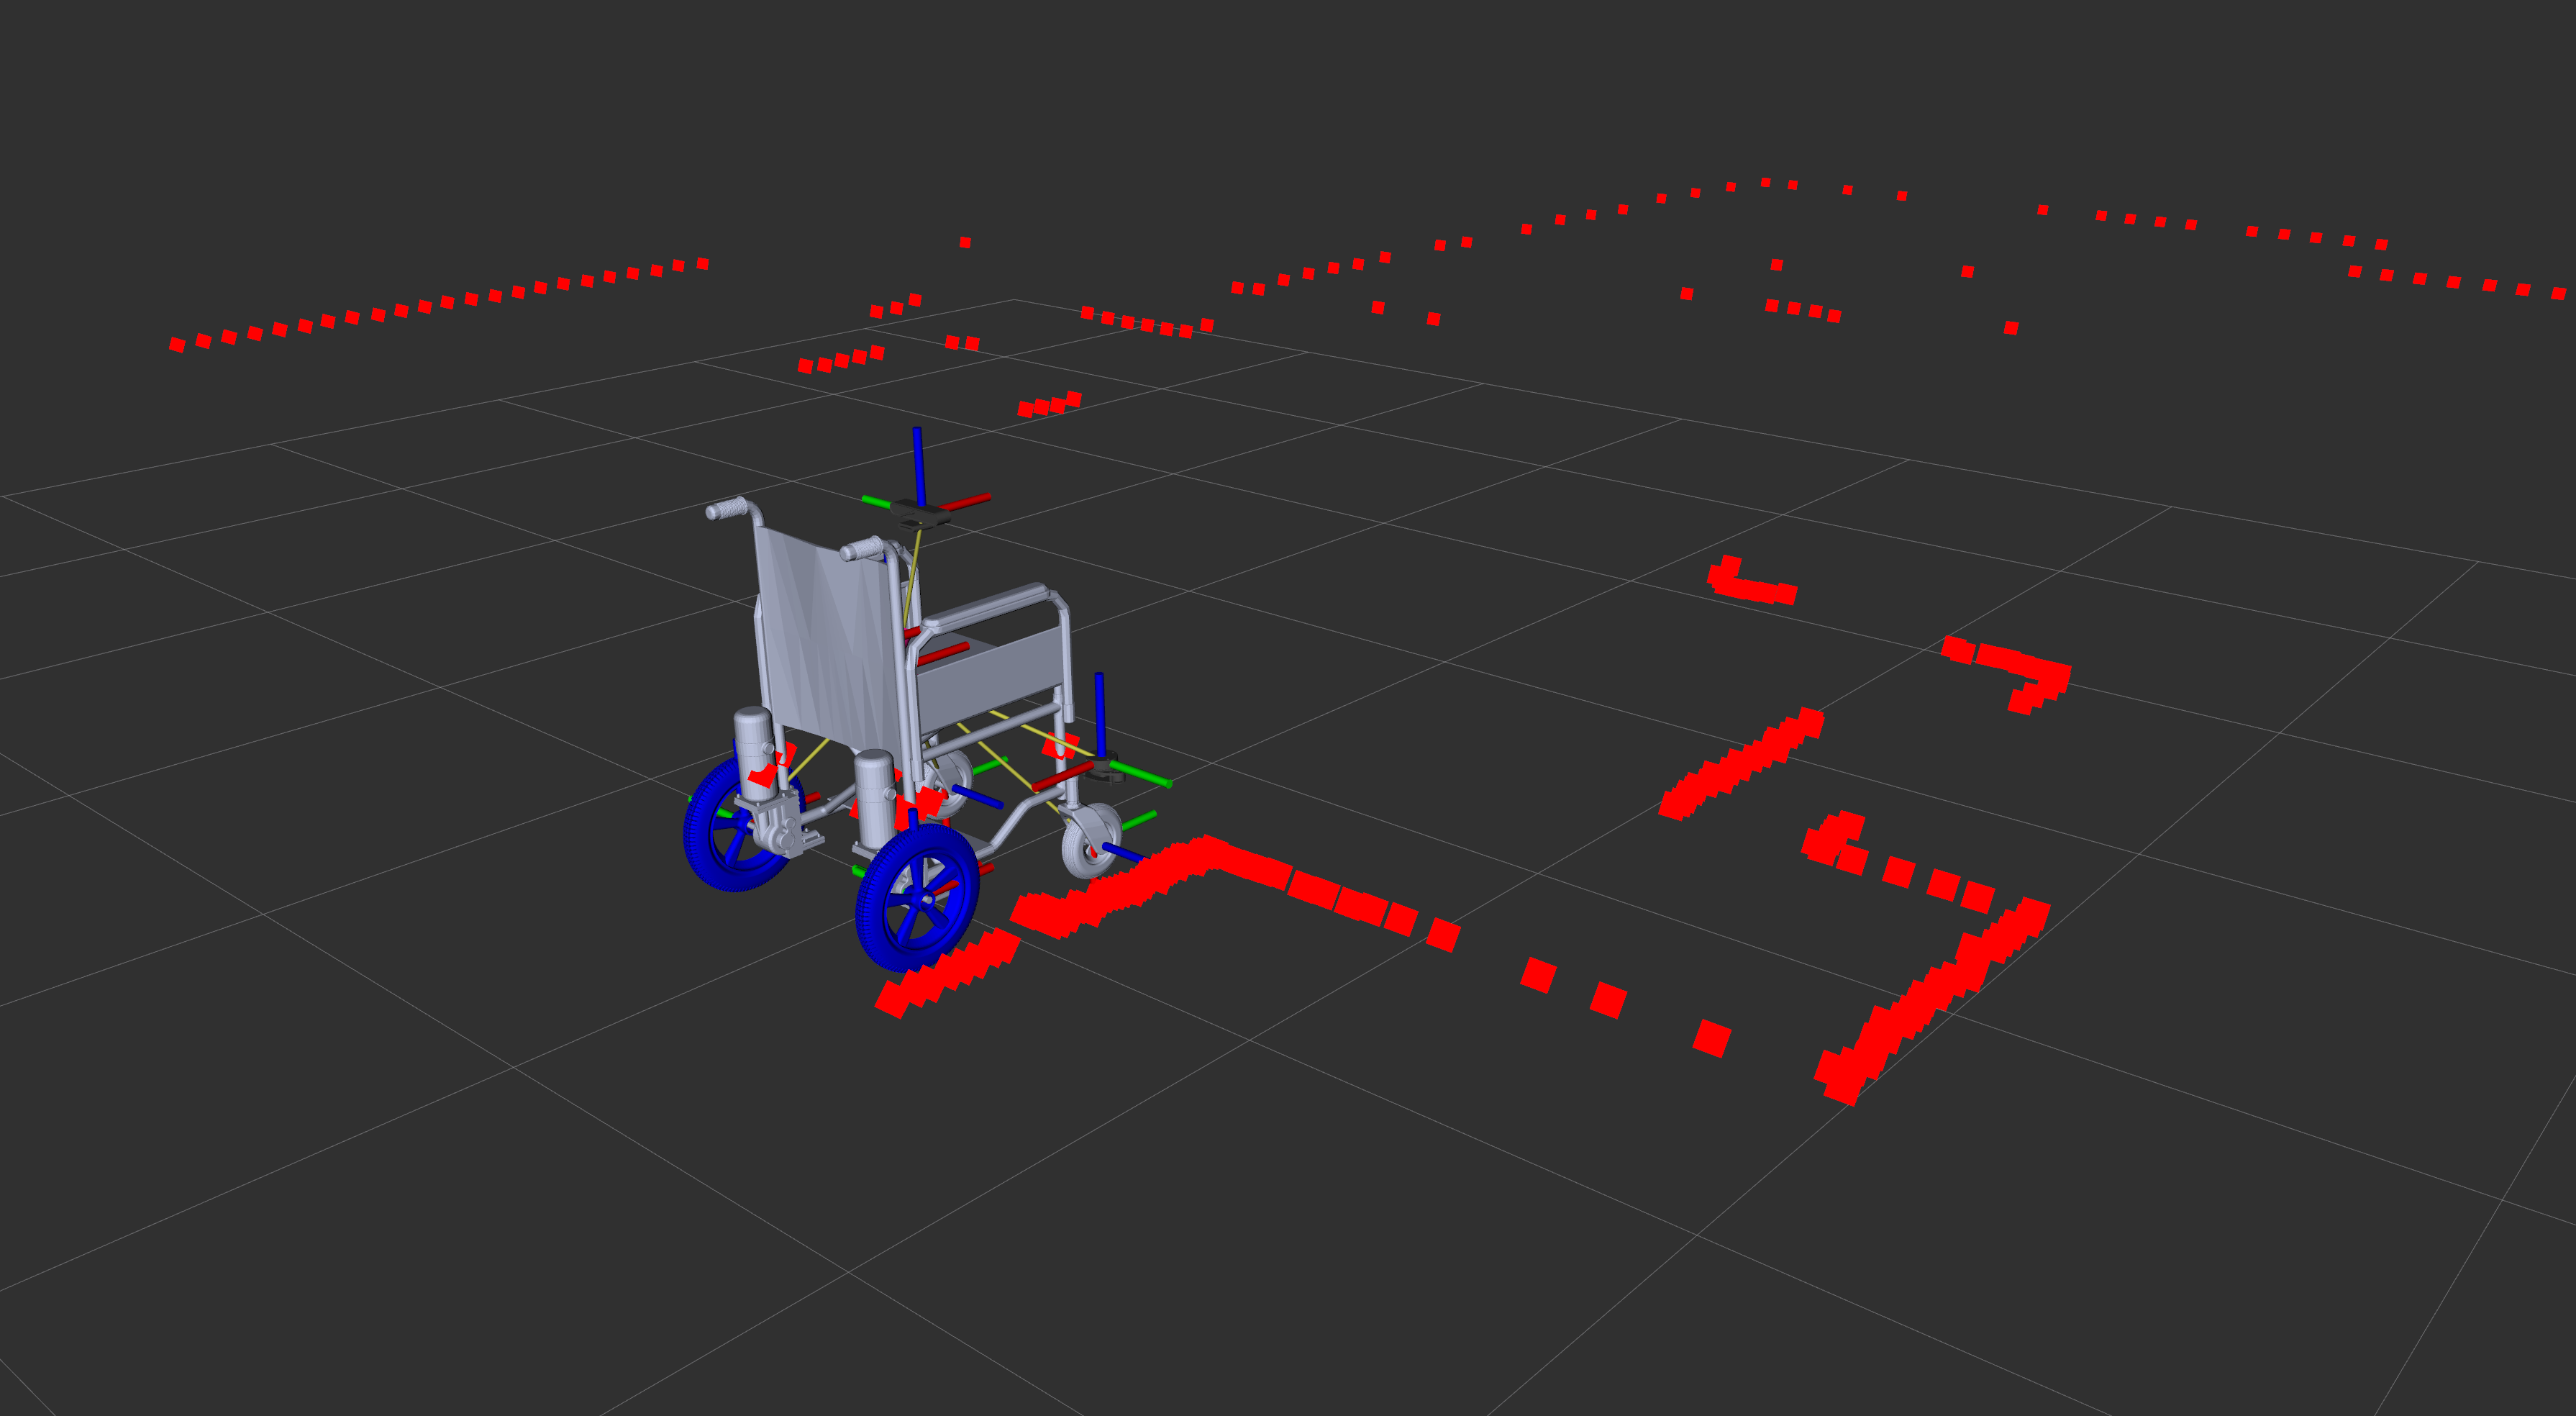
\includegraphics[width=\linewidth]{figures/ch04/lidar_issue.png}
    \caption{RViz view of the robot model with a single raw LiDAR scan. Self-obstruction arcs caused by the chassis are clearly visible as dense point clusters around the robot body.}
    \label{fig:rviz_single_lidar_model}
\end{minipage}
\hfill
\begin{minipage}{0.48\textwidth}
    \centering
    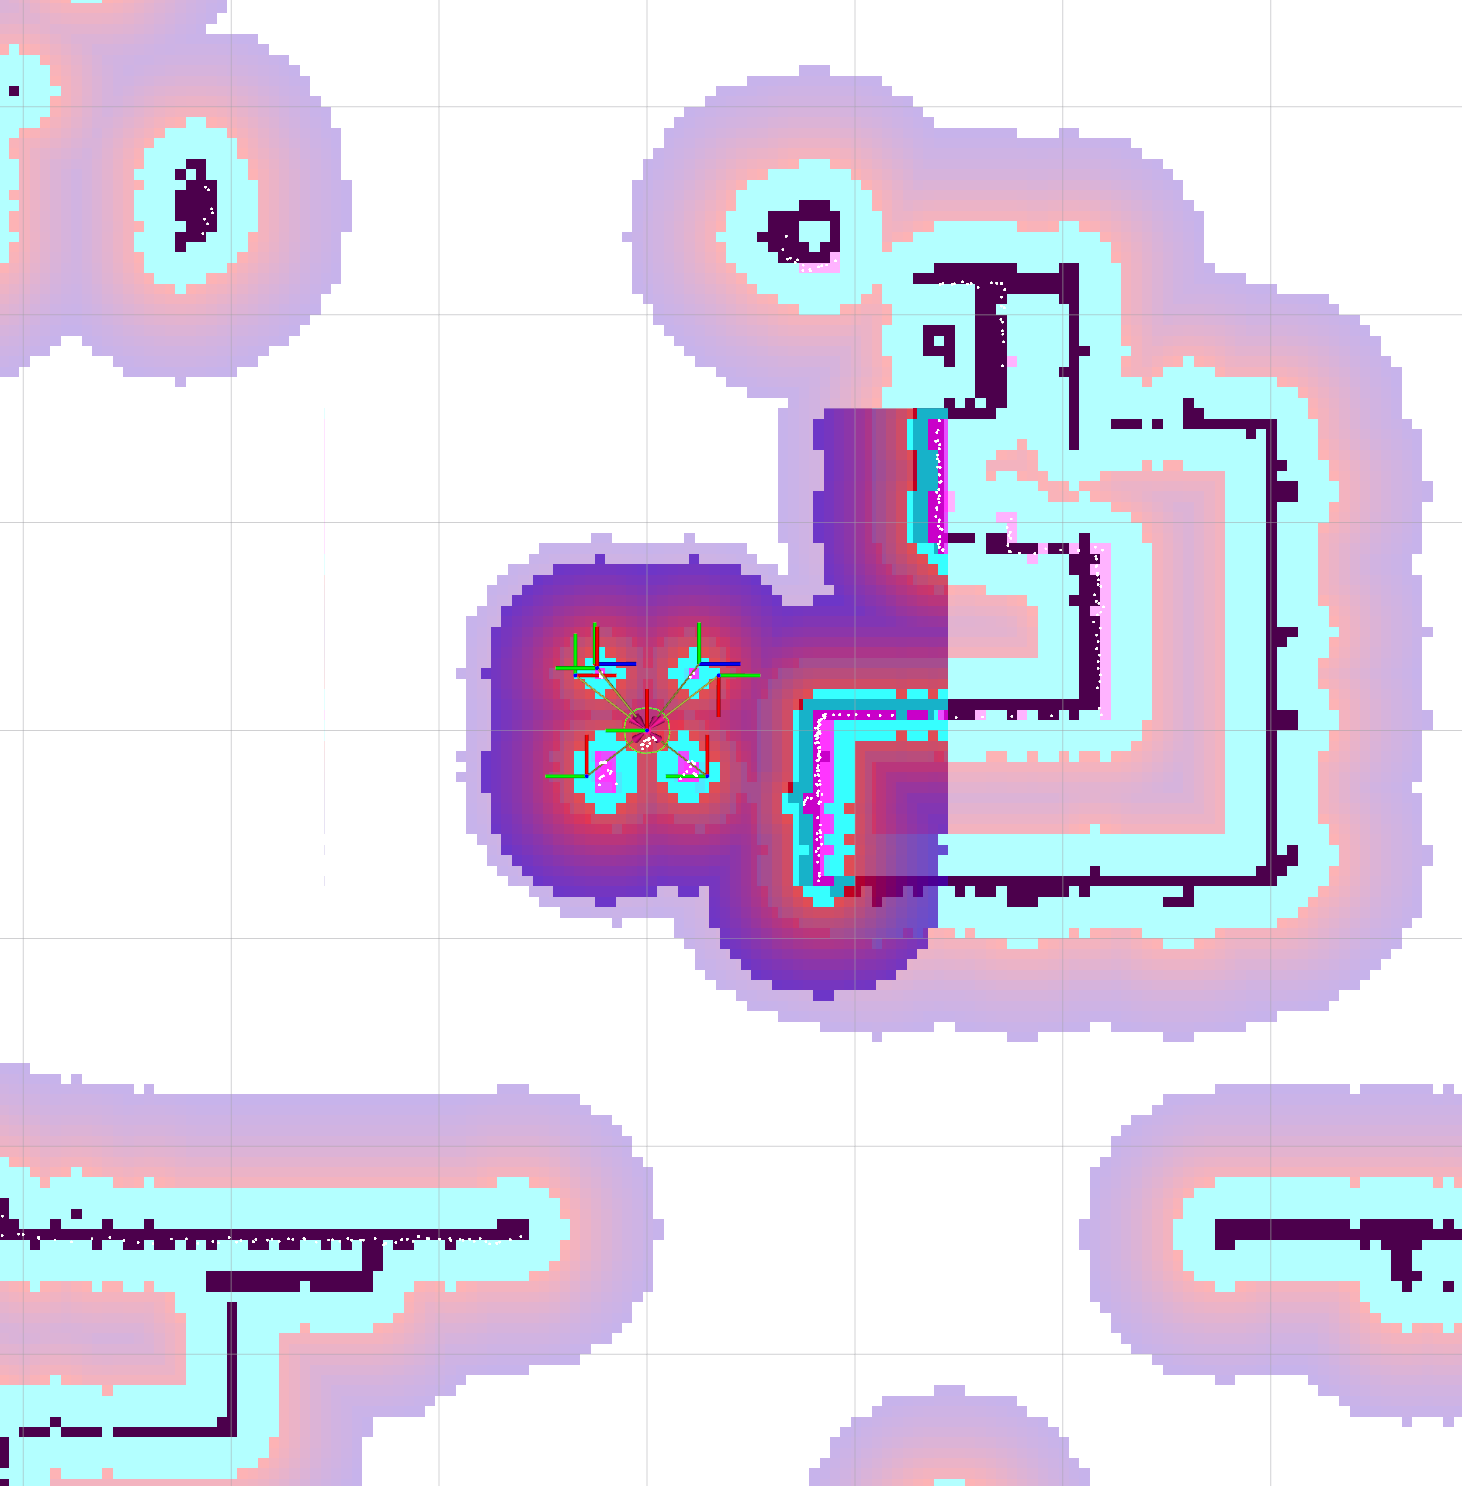
\includegraphics[width=\linewidth]{figures/ch04/lidar_issue_costmap.png}
    \caption{RViz local costmap before applying the crop filter. The phantom lethal ring caused by wheelchair-frame self-obstruction surrounds the robot footprint, causing the planner to treat the robot itself as an obstacle.}
    \label{fig:rviz_costmap_self_obstruction}
\end{minipage}
\end{figure}


The cropping boundaries are configured in \texttt{laser\_left\_filter.yaml} and \texttt{laser\_right\_filter.yaml}. The left sensor crops out the wheelchair body by maintaining angles from $0.20$ to $4.915$ radians. The right sensor filters angles from $0.0$ to $4.60$ radians. Table~\ref{tab:laser_filters} details the key parameters of both angular cropping filters.

\begin{table}[H]
\centering
\caption{LiDAR scan cropping angular filter parameters (\texttt{laser\_left\_filter.yaml}, \texttt{laser\_right\_filter.yaml}).}
\label{tab:laser_filters}
\renewcommand{\arraystretch}{1.2}
\begin{tabular}{lll}
\toprule
\textbf{Parameter} & \textbf{Left LiDAR} & \textbf{Right LiDAR} \\
\midrule
Filter Type & \texttt{LaserScanAngularBoundsFilter} & \texttt{LaserScanAngularBoundsFilter} \\
\texttt{lower\_angle} & $0.200$~rad & $0.000$~rad \\
\texttt{upper\_angle} & $4.915$~rad & $4.600$~rad \\
\bottomrule
\end{tabular}
\end{table}

\subsection{Phase 2: Dual LiDAR Scan Fusion}

Cropping out the self-obstruction zones left a large angular dead zone (almost 180 degrees) behind and to the sides of the robot, as the patient's body and high backrest blocked the laser beams. Navigating with a single LiDAR was hazardous during backward movements or tight turns.

To minimize blind spots, a dual-LiDAR setup was implemented using two LD06 units. The first LiDAR is mounted on the front-left corner of the wheelchair and the second on the rear-right corner, so their combined fields of view wrap around the robot body. Both scans are independently processed by the angular filters described above, then a C++ node from the \texttt{dual\_laser\_merger} package fuses both filtered scans into a single, unified \texttt{/scan} topic.

\begin{figure}[H]
\centering
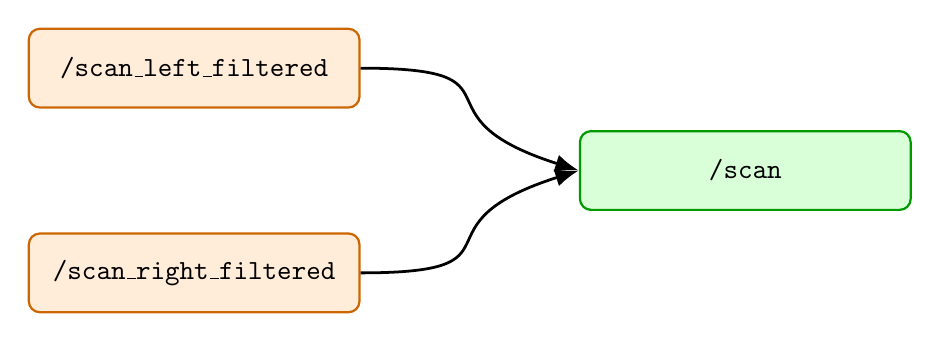
\begin{tikzpicture}[
    >=Latex,
    thick,
    topic/.style={
        draw,
        rounded corners=4pt,
        minimum width=4.2cm,
        minimum height=1cm,
        font=\ttfamily,
        align=center
    },
    input/.style={
        topic,
        draw=orange!80!black,
        fill=orange!15
    },
    output/.style={
        topic,
        draw=green!60!black,
        fill=green!15
    }
]

% Input topics
\node[input] (left) at (0,1.3) {/scan\_left\_filtered};
\node[input] (right) at (0,-1.3) {/scan\_right\_filtered};

% Output topic
\node[output] (scan) at (7,0) {/scan};

% Curved arrows
\draw[-{Latex[length=3mm]}, line width=1pt]
(left.east) .. controls +(2.2,0) and +(-2.2,0.7) .. (scan.west);

\draw[-{Latex[length=3mm]}, line width=1pt]
(right.east) .. controls +(2.2,0) and +(-2.2,-0.7) .. (scan.west);

\end{tikzpicture}
\caption{Dual filtered LiDAR scans are merged into a single scan topic.}
\label{fig:scan_merger_block}
\end{figure}
% --- Two LiDARs: robot model with both sensors + merged costmap ---\begin{figure}[H]
\begin{figure}[H]
\centering
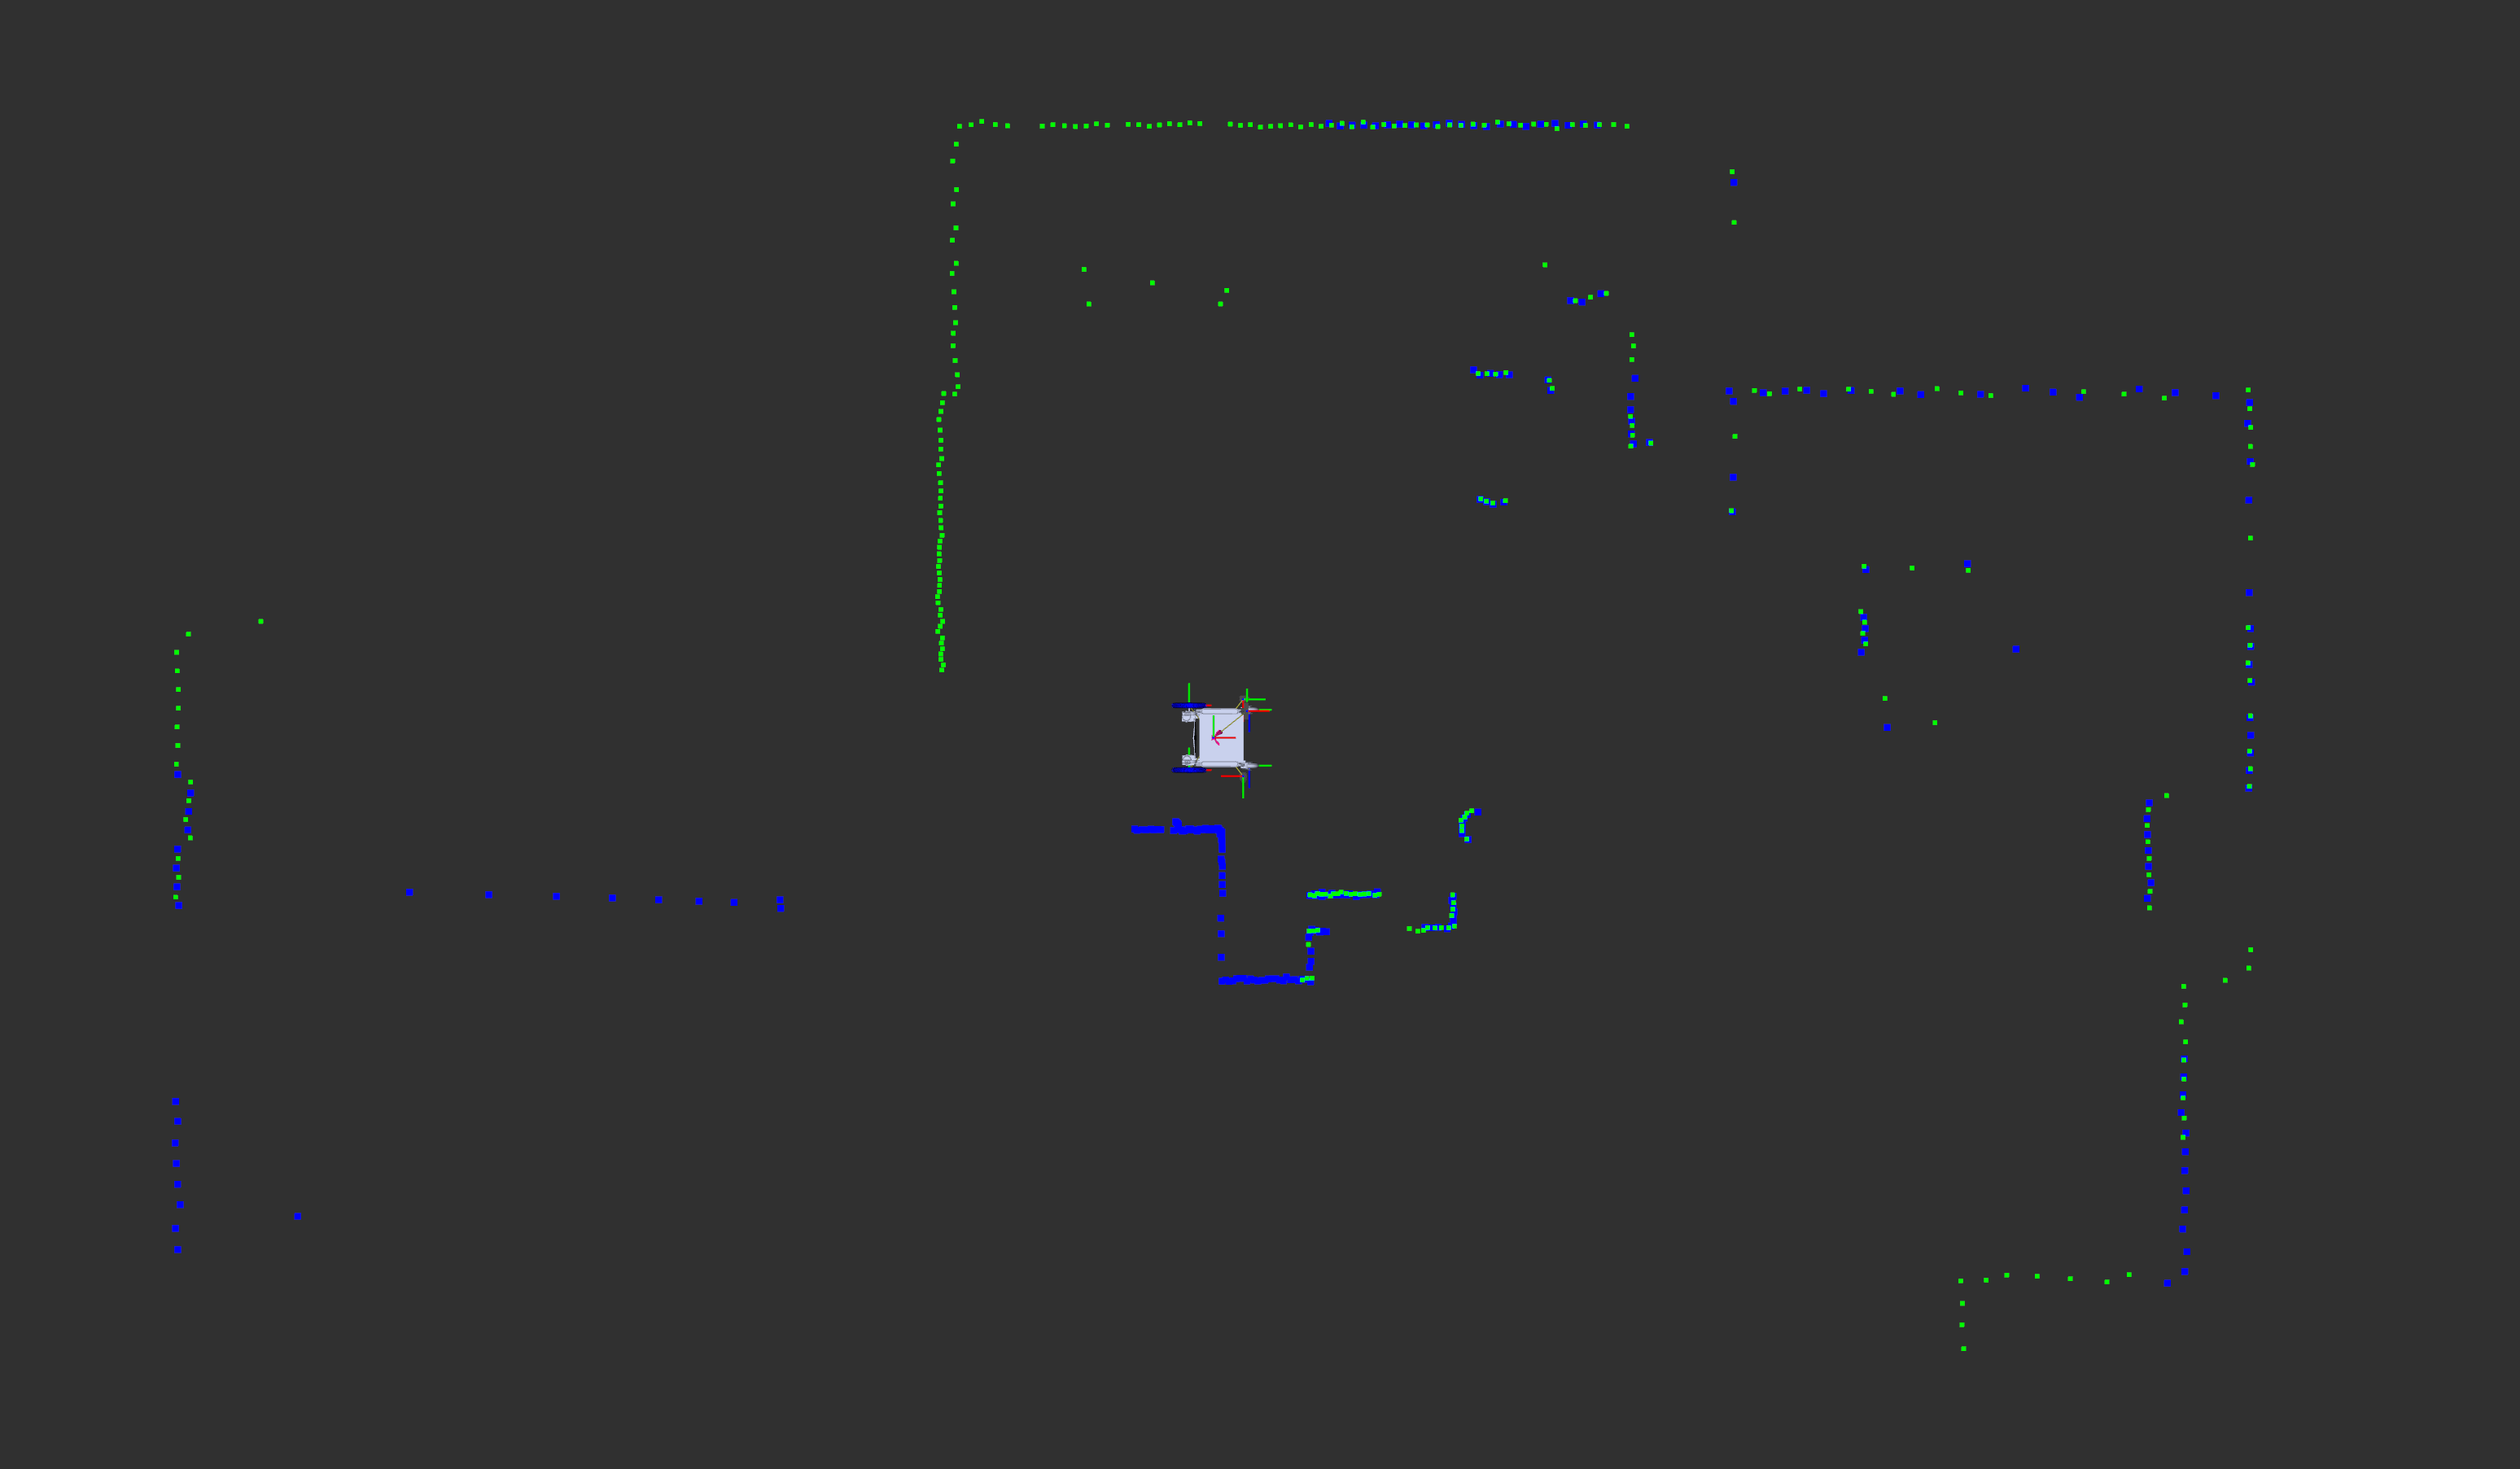
\includegraphics[width=\textwidth]{figures/ch04/left_right_laser.png}
\caption{RViz view of the robot model with both independently filtered LiDAR scans. The two sensors (front-left and rear-right) are rendered in distinct colours, illustrating their complementary angular coverage.}
\label{fig:rviz_dual_lidar_model}
\end{figure}

\begin{figure}[H]
\centering
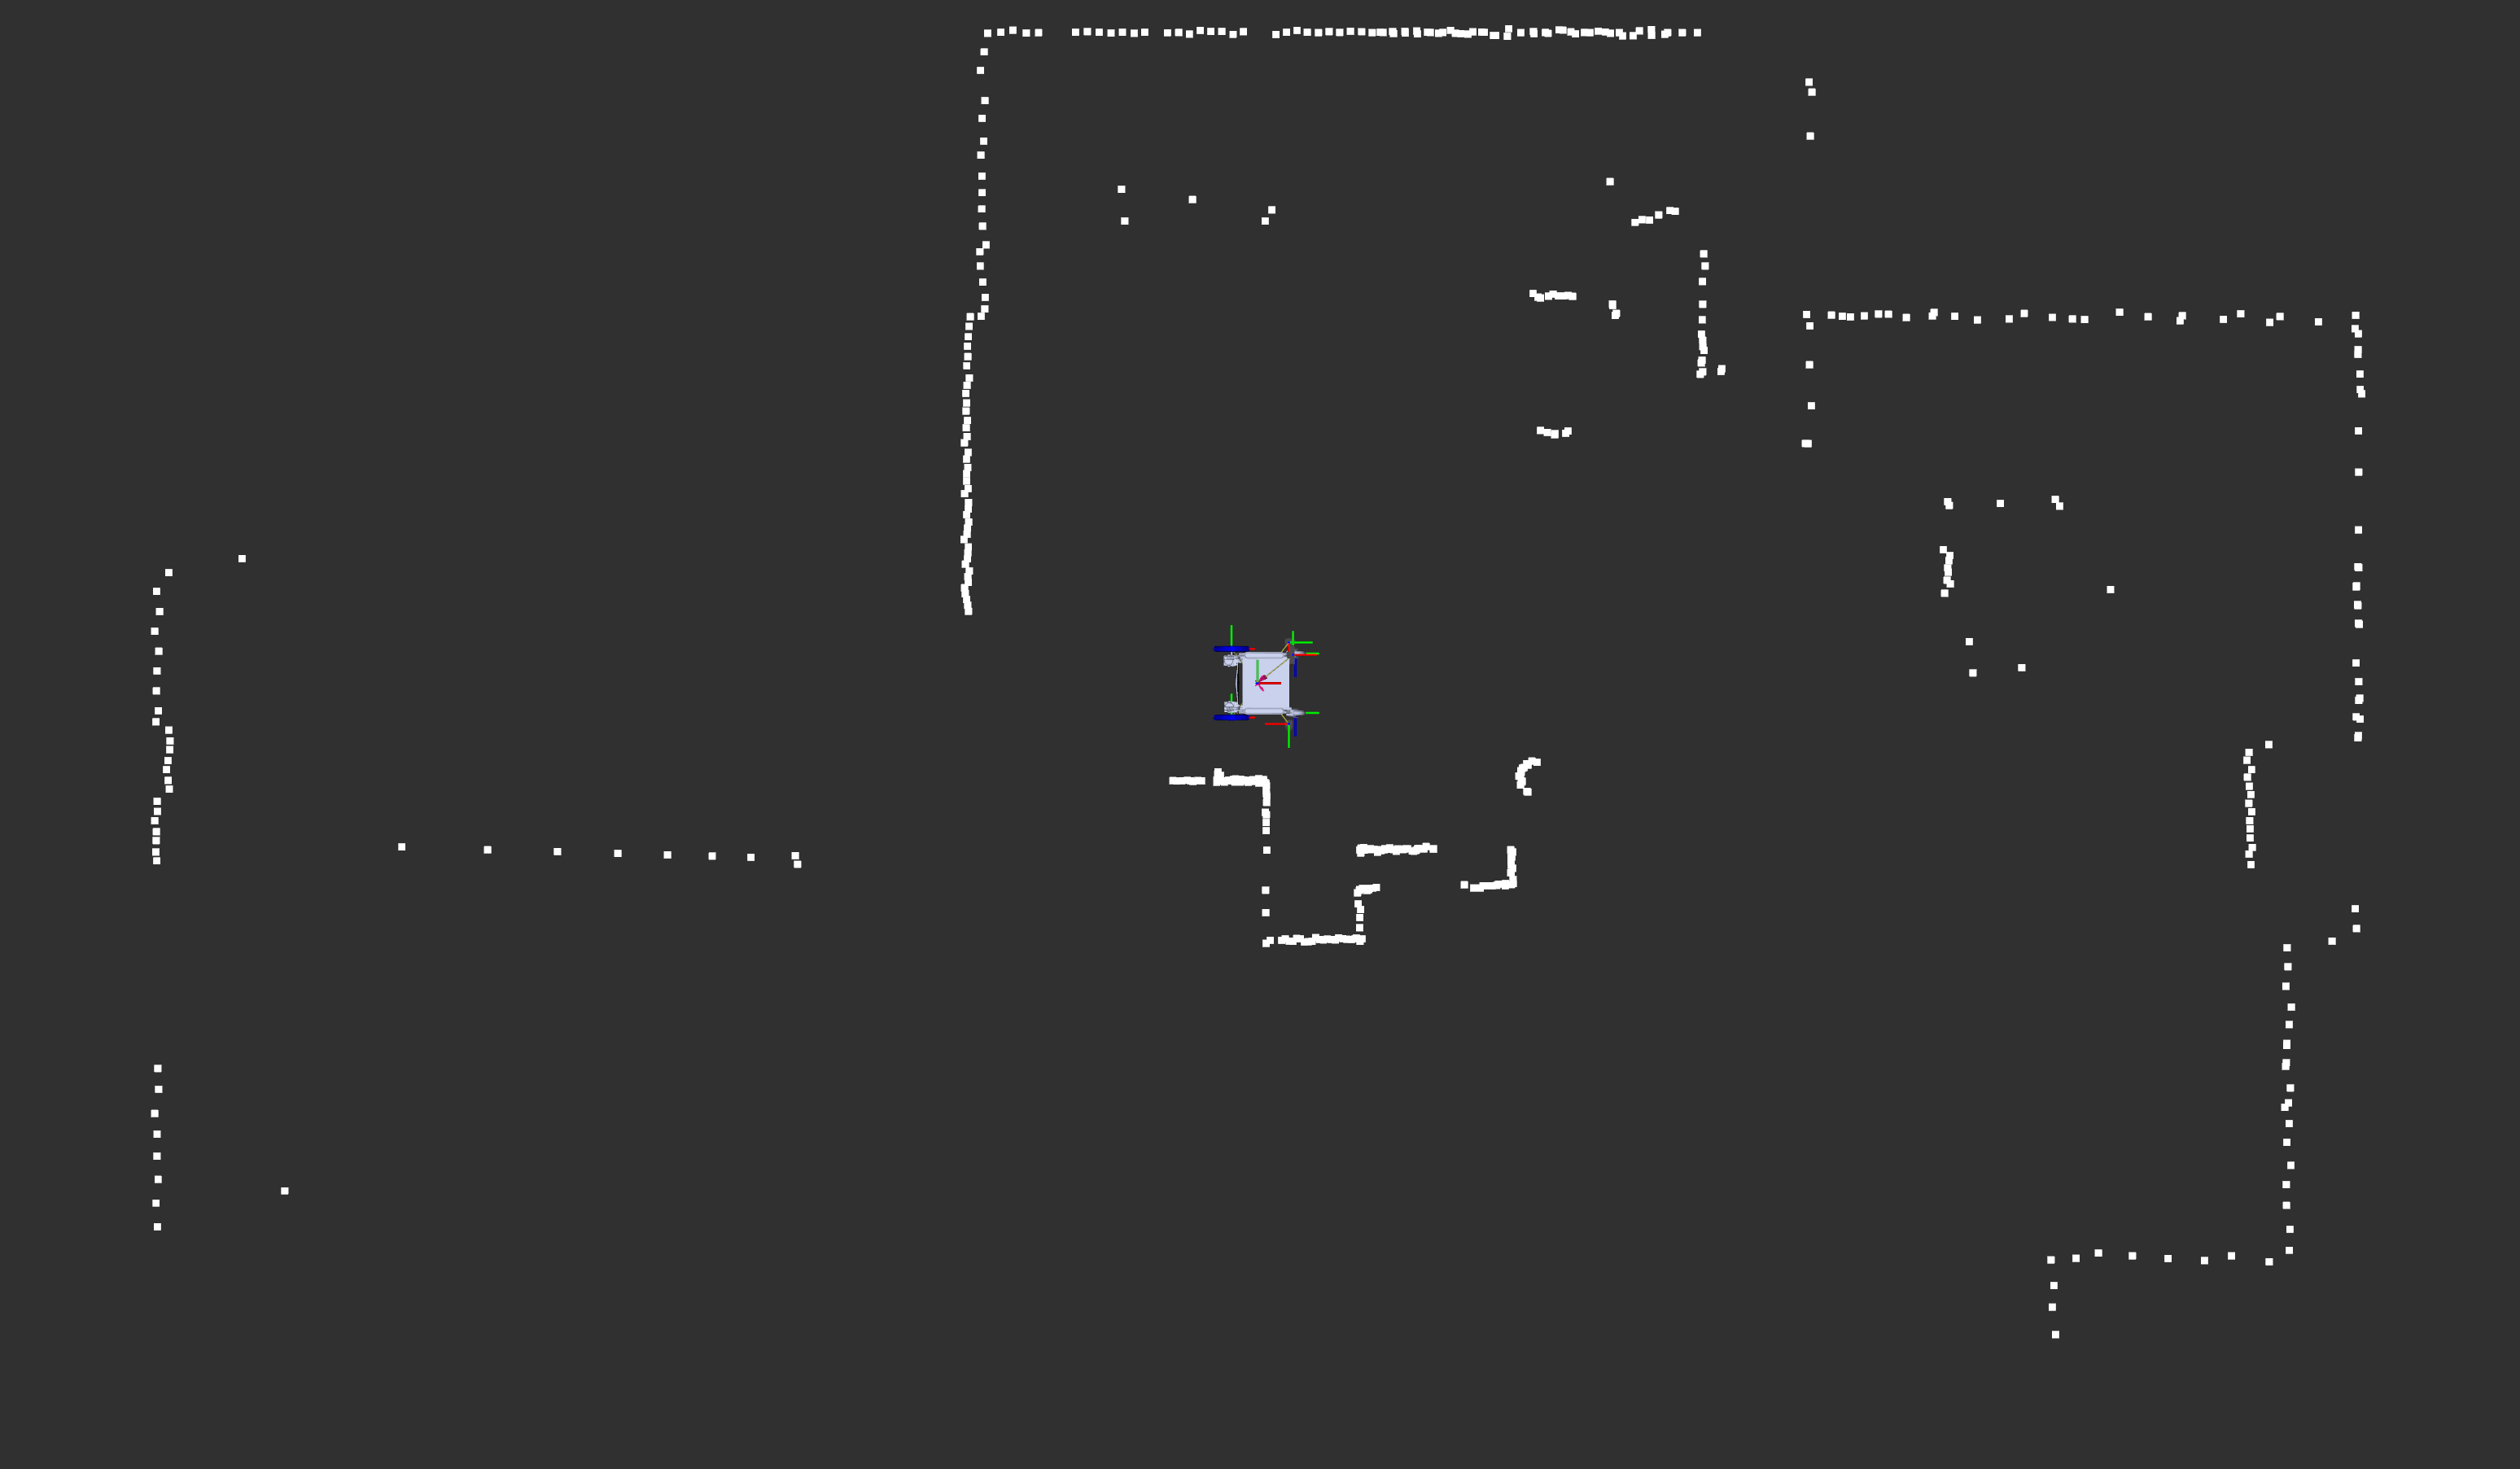
\includegraphics[width=\textwidth]{figures/ch04/merged_laser.png}
\caption{RViz local costmap built from the merged \texttt{/scan} topic. Near-360\textdegree{} obstacle marking is achieved, eliminating the blind zone that a single rear-mounted or front-mounted LiDAR would leave.}
\label{fig:rviz_merged_costmap}
\end{figure}

The merger node (configured in \texttt{dual\_laser\_merger.yaml}) listens to \texttt{/scan\_left\_filtered} and \texttt{/scan\_right\_filtered}, aligns them to the \texttt{base\_link} frame using TF transforms, and outputs a merged \texttt{/scan} message. The resulting scan covers approximately 330 degrees, resolving the blind spot issue.

\begin{figure}[H]
    \centering
    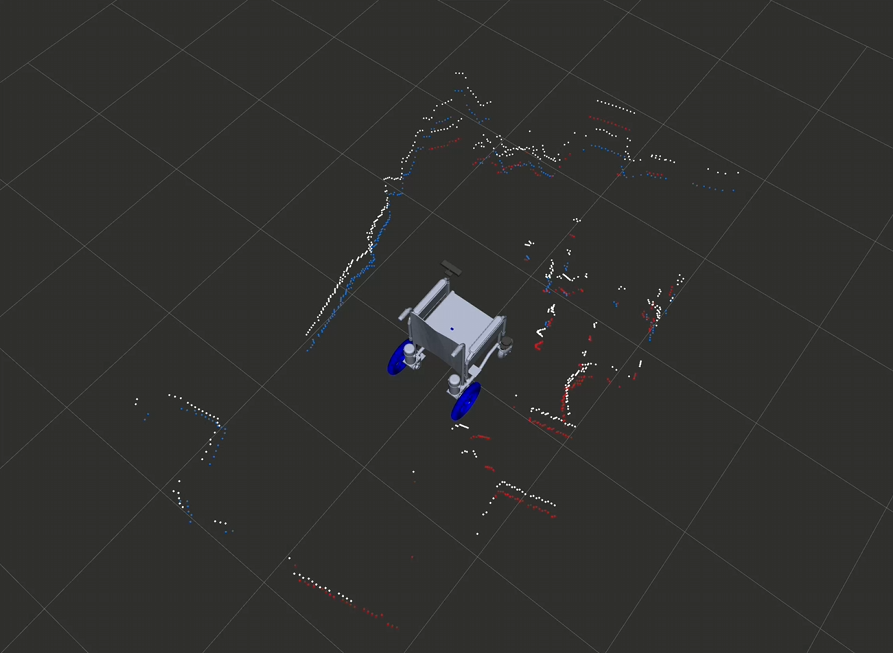
\includegraphics[width=1\textwidth]{figures/ch04/real_lidar_merge.png}
    \caption{Real-world demonstration of merging dual LiDAR scans during wheelchair operation.}
    \label{fig:real_lidar_merge}
\end{figure}


Table~\ref{tab:dual_merger_yaml} summarizes the essential configuration parameters of the merger node.

\begin{table}[H]
\centering
\caption{Dual laser merger node parameters (\texttt{dual\_laser\_merger.yaml}).}
\label{tab:dual_merger_yaml}
\renewcommand{\arraystretch}{1.2}
\begin{tabular}{ll}
\toprule
\textbf{Parameter} & \textbf{Value} \\
\midrule
\texttt{laser\_1\_topic} & \texttt{/scan\_left\_filtered} \\
\texttt{laser\_2\_topic} & \texttt{/scan\_right\_filtered} \\
\texttt{merged\_scan\_topic} & \texttt{/scan} \\
\texttt{target\_frame} & \texttt{base\_link} \\
\texttt{range\_min} / \texttt{range\_max} & $0.01$~m / $25.0$~m \\
\texttt{angle\_min} / \texttt{angle\_max} & $-\pi$ / $+\pi$~rad \\
\texttt{angle\_increment} & $0.001$~rad \\
\texttt{scan\_time} & $0.067$~s \\
\texttt{allowed\_radius} & $0.45$~m \\
\bottomrule
\end{tabular}
\end{table}

\section{Block 3: State Estimation \& Odometry Fusion}
\subsection{LiDAR–Depth Camera Sensor Fusion}

\subsection{Overview and Motivation}
\label{sec:overview_motivation}

Reliable obstacle perception is a fundamental requirement for autonomous
navigation in assistive mobile robots. Since the proposed smart wheelchair
operates in dynamic indoor environments — homes, hospitals, and educational
buildings — it must accurately detect obstacles of varying sizes, heights,
and distances to ensure safe navigation. Relying on a single sensing
modality is insufficient because each sensor possesses inherent limitations
that can compromise navigation reliability.

\begin{table}[H]
    \centering
    \caption{Complementary characteristics of LiDAR and RGB-D sensors.}
    \label{tab:sensor_limitations}
    \begin{tabular}{|l|p{0.38\linewidth}|p{0.4\linewidth}|}
    \hline
    \textbf{Sensor} & \textbf{Strengths} & \textbf{Limitations} \\
    \hline
    \textbf{2D LiDAR} & Highly accurate, long-range distance measurements. & Scans only a single horizontal plane; misses overhanging tables or low floor objects. \\
    \hline
    \textbf{RGB-D Camera} & Dense 3D volumetric perception with a wide vertical field of view. & Depth accuracy degrades over distance due to stereo matching uncertainty and noise. \\
    \hline
    \end{tabular}
\end{table}

To overcome these complementary limitations, this work presents a sensor
fusion framework that combines the geometric accuracy of the 2D LiDAR with
the volumetric perception of the RGB-D camera. An offline depth-bias
calibration stage first compensates for systematic measurement errors in the
camera; the corrected data are then fused in real time using a range-adaptive
confidence weighting strategy. The resulting fused laser scan is supplied
directly to the ROS~2 Nav2 navigation stack, providing richer environmental
information for obstacle avoidance and path planning. The approach is inspired
by Delhibabu et al.~\cite{delhibabu2026}, and extends their occupancy-map
framework into a complete assistive robotics pipeline with a native ROS~2
implementation optimized for real-time wheelchair navigation.

\begin{figure}[H]
    \centering
    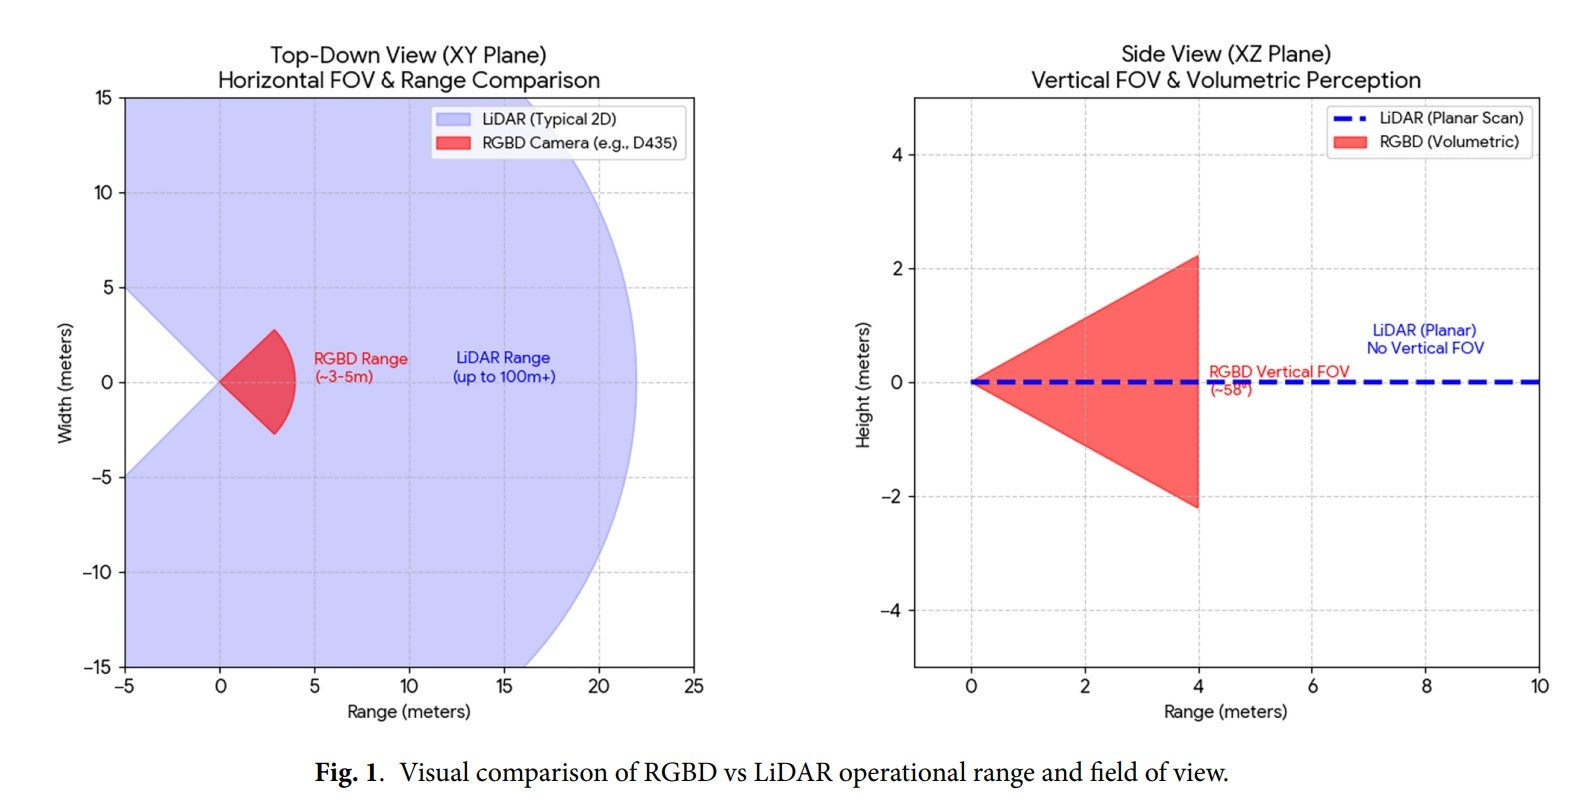
\includegraphics[width=1.0\linewidth]{figures/ch04/lidar_camera_comparison.jpg}
    \caption{Visual comparison between LiDAR and RGB-D sensing modalities.}
    \label{fig:lidar_camera_comparison}
\end{figure}

\subsection{Depth Bias Calibration}

\subsubsection{Problem and Approach}

RGB-D cameras such as the Orbbec Astra Pro estimate depth through
structured infrared light projection onto the scene, with depth inferred
from the deformation of the projected pattern. Although this approach
provides dense three-dimensional measurements at low cost, it introduces
a systematic depth bias — a consistent, reproducible offset between the
reported and true distance to a surface — arising from lens distortion,
calibration imperfections in the infrared projector and receiver, and
quantization error in the depth computation. Unlike random noise,
systematic bias persists regardless of how many frames are averaged and
must therefore be explicitly measured and corrected prior to fusion.

The calibration approach adopted in this work exploits the
complementary accuracy characteristics of the two onboard sensors.
The 2D LiDAR operates on the time-of-flight principle and achieves
sub-centimetre ranging accuracy at typical indoor distances, making it
a reliable ground-truth reference. By simultaneously observing the
same planar surface with both sensors, the systematic offset of the
RGB-D camera can be isolated and quantified. The procedure follows the
calibration algorithm proposed by Delhibabu et al.~\cite{delhibabu2026},
adapted to the sensor configuration of this platform.

%---------------------------------------------------------------
\subsubsection{Calibration Procedure}
%---------------------------------------------------------------

The robot is positioned one to three metres in front of a flat
vertical wall. A synchronized (LiDAR, PointCloud2) frame pair is
processed on each callback until $N = 10$ valid bias samples have
been collected, at which point their mean is published and persisted.
Algorithm~\ref{alg:calibration} summarises the procedure.

\begin{algorithm}[htbp]
\caption{RANSAC Depth-Bias Calibration}
\label{alg:calibration}
\begin{algorithmic}[1]
\renewcommand{\algorithmicrequire}{\textbf{Input:}}
\renewcommand{\algorithmicensure}{\textbf{Output:}}
\REQUIRE Synchronized LiDAR scan $L$, RGB-D cloud $C$, rotation $R$, translation $\mathbf{t}$ (camera $\rightarrow$ \texttt{base\_footprint}), required sample count $N$
\ENSURE Depth bias offset $\Delta z$

\STATE $S \leftarrow [\,]$
\WHILE{$|S| < N$}
    \STATE Receive synchronized frame pair $(L, C)$
    \STATE Extract frontal LiDAR points within $\pm\alpha^{\circ} \rightarrow P_{\text{lidar}}$
    \STATE Apply RANSAC line fit to $P_{\text{lidar}} \rightarrow$ ground-truth distance $z_{\text{gt}}$ \quad (discard frame on failure)
    \STATE Transform $C$ into \texttt{base\_footprint}: $C' = RC^{\top} + \mathbf{t}$
    \STATE Filter $C'$ by height $[z_{\min}, z_{\max}]$ and frontal cone $\pm\beta^{\circ} \rightarrow$ median depth $z_{\text{meas}}$ \quad (discard frame on failure)
    \STATE Append $\delta = z_{\text{gt}} - z_{\text{meas}}$ to $S$
\ENDWHILE

\STATE $\Delta z \leftarrow \text{mean}(S)$
\STATE Persist $\Delta z$ and $\text{std}(S)$ to \texttt{calibration.json}
\STATE Publish $\Delta z$ on \texttt{/depth\_bias} with \texttt{TRANSIENT\_LOCAL} durability
\end{algorithmic}
\end{algorithm}

Each iteration incorporates explicit failure checks; frames in which
either sensor fails to observe the wall clearly are silently discarded
rather than contributing a corrupted sample. Averaging ten independent
samples reduces the influence of per-frame sensor perturbations while
keeping calibration time practical.

%---------------------------------------------------------------
\subsubsection{LiDAR Wall Detection}
%---------------------------------------------------------------

Frontal LiDAR points within $\pm 25^{\circ}$ of the forward axis are
extracted and converted from polar to Cartesian coordinates. A line is
then fit to these points using RANSAC~\cite{delhibabu2026}. The
candidate line is expressed in unit-normal implicit form

\begin{equation}
    ax + by + c = 0, \qquad \sqrt{a^{2}+b^{2}} = 1,
    \label{eq:line}
\end{equation}

so that the perpendicular distance from the sensor origin to the wall
follows directly as $|c|$, with no additional division required.
Table~\ref{tab:ransac} lists the parameter values used.

\begin{table}[H]
\centering
\caption{RANSAC wall-detection parameters}
\label{tab:ransac}
\begin{tabular}{llll}
\hline
\textbf{Parameter} & \textbf{Value} & \textbf{Rationale} \\
\hline
Iterations $K$          & 150     & ${>}99\%$ success at ${\leq}50\%$ outlier rate \\
Inlier threshold $\varepsilon$ & 0.03\,m & Consistent with LiDAR noise spec \\
Minimum inliers $M$     & 8       & Prevents degenerate fits \\
Frontal half-angle $\alpha$ & $25^{\circ}$ & Balances coverage and clutter rejection \\
\hline
\end{tabular}
\end{table}

%---------------------------------------------------------------
\subsubsection{RGB-D Depth Measurement and Bias Computation}
%---------------------------------------------------------------

The point cloud is transformed into the \texttt{base\_footprint} frame
via $\mathbf{p}' = R\mathbf{p} + \mathbf{t}$, where $R$ and
$\mathbf{t}$ are obtained from the TF tree at the message timestamp.
Points outside the height band $[0.1,\,2.0]$\,m and outside a
$\pm 15^{\circ}$ frontal cone are discarded. The representative camera
depth is taken as the median two-dimensional ground-plane range of the
surviving points,

\begin{equation}
    z_{\text{meas}} = \operatorname{median}
        \!\left(\sqrt{x_{i}^{\prime\,2} + y_{i}^{\prime\,2}}\right),
    \label{eq:zmeas}
\end{equation}

with the median preferred over the mean for robustness to the
heavy-tailed error distribution of structured-light sensors. The
per-frame bias sample is $\delta = z_{\text{gt}} - z_{\text{meas}}$,
and after $N$ samples the calibration offset and its standard deviation
are

\begin{equation}
    \Delta z = \frac{1}{N}\sum_{k=1}^{N}\delta_{k},
    \qquad
    \sigma_{\Delta z} =
        \sqrt{\frac{1}{N}\sum_{k=1}^{N}(\delta_{k}-\Delta z)^{2}}.
    \label{eq:bias}
\end{equation}

The result is written atomically to \texttt{calibration.json} using a
write-then-rename strategy — ensuring a power-loss event cannot corrupt
a previously valid calibration — and published on \texttt{/depth\_bias}
with \textsc{Transient\_Local} durability so that late-joining nodes
receive the value immediately upon subscription.

%%%%%%%%%%%%%%%%%%%%%%%%%%%%%%%%%%%%%%%%%%%%%%%%%%%%%%%%%%%%%%%%%%%
\subsection{Real-Time Sensor Fusion}
%%%%%%%%%%%%%%%%%%%%%%%%%%%%%%%%%%%%%%%%%%%%%%%%%%%%%%%%%%%%%%%%%%%

%---------------------------------------------------------------
\subsubsection{Pipeline Overview}
%---------------------------------------------------------------

The fusion node runs continuously during robot operation, consuming
synchronized LiDAR and RGB-D frames and publishing a fused
\texttt{sensor\_msgs/LaserScan} on \texttt{/fused\_scan} at the rate
of the slower sensor. Figure~\ref{fig:fusion_pipeline} illustrates the
processing stages. The design philosophy prioritises safety over
completeness: the node never blocks navigation while waiting for
calibration data, degrades gracefully to LiDAR-only output when camera
data is unavailable, and drops individual frames silently rather than
publishing a result of uncertain quality.

\begin{figure}[H]
\centering
% Replace with your actual TikZ diagram or \includegraphics
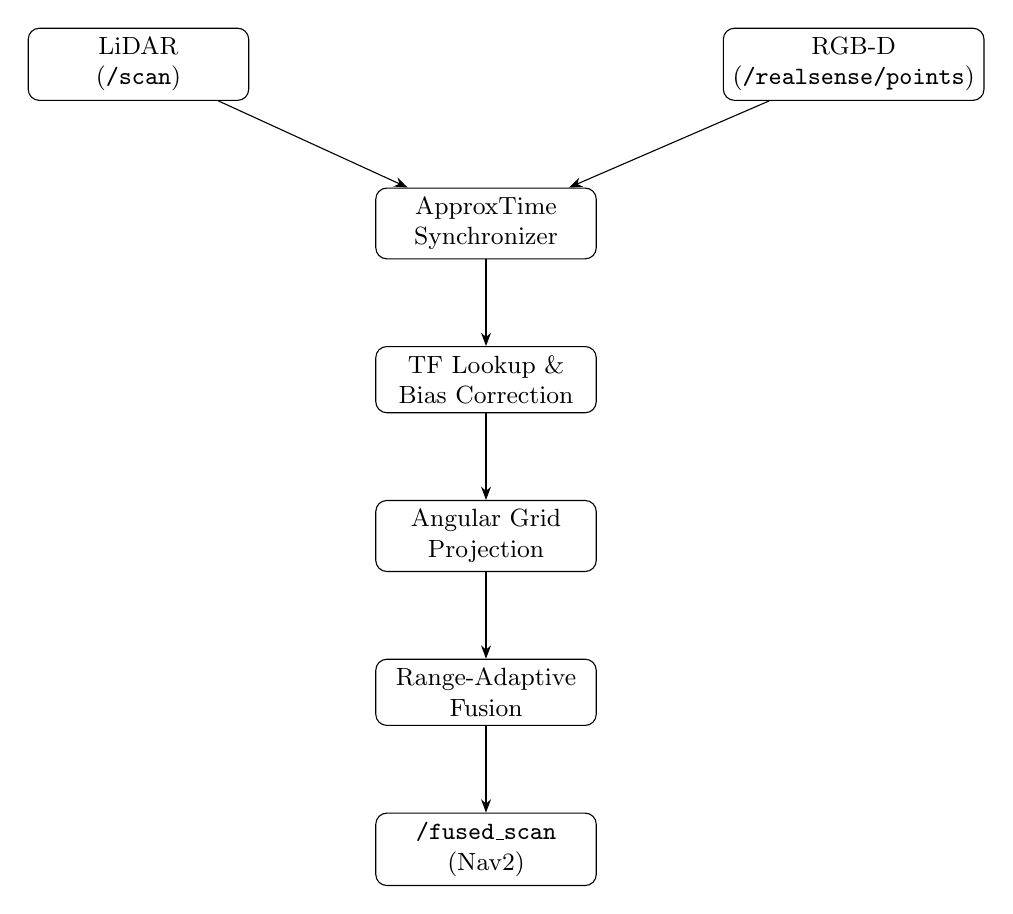
\begin{tikzpicture}[
    node distance=1.1cm and 1.6cm,
    box/.style={draw, rounded corners, minimum width=2.8cm,
                minimum height=0.7cm, align=center, font=\small},
    arr/.style={-Stealth}
]
\node[box] (sync)   {ApproxTime\\Synchronizer};
\node[box, above left=of sync]  (lidar) {LiDAR\\(\texttt{/scan})};
\node[box, above right=of sync] (rgbd)  {RGB-D\\(\texttt{/realsense/points})};
\node[box, below=of sync]       (tf)    {TF Lookup \&\\Bias Correction};
\node[box, below=of tf]         (proj)  {Angular Grid\\Projection};
\node[box, below=of proj]       (fuse)  {Range-Adaptive\\Fusion};
\node[box, below=of fuse]       (pub)   {\texttt{/fused\_scan}\\(Nav2)};

\draw[arr] (lidar) -- (sync);
\draw[arr] (rgbd)  -- (sync);
\draw[arr] (sync)  -- (tf);
\draw[arr] (tf)    -- (proj);
\draw[arr] (proj)  -- (fuse);
\draw[arr] (fuse)  -- (pub);
\end{tikzpicture}
\caption{Fusion node processing pipeline.}
\label{fig:fusion_pipeline}
\end{figure}

%---------------------------------------------------------------
\subsubsection{Temporal Synchronization}
%---------------------------------------------------------------

The LiDAR and RGB-D camera publish at different independent rates —
typically 10\,Hz and 30\,Hz respectively. Naively pairing the most
recently received message from each sensor would introduce a temporal
mismatch; at a robot velocity of 0.3\,m/s and a 100\,ms offset this
amounts to a 3\,cm positional error before any sensor noise is
considered. Both streams are therefore passed through ROS\,2's
\texttt{ApproximateTimeSynchronizer}, which emits a callback only when
a pair of messages satisfies $|t_{\text{lidar}} - t_{\text{rgbd}}| 
t_{\text{slop}}$, with $t_{\text{slop}} = 1.0$\,s. The timestamp of
the LiDAR message is propagated to the output scan header so that
downstream TF lookups reference the correct robot pose at the time of
measurement.

%---------------------------------------------------------------
\subsubsection{Coordinate Transformation and Bias Correction}
%---------------------------------------------------------------

The RGB-D point cloud arrives in the camera optical frame and must be
transformed into \texttt{base\_footprint} before comparison with the
LiDAR:

\begin{equation}
    \mathbf{p}' = R\,\mathbf{p} + \mathbf{t},
    \label{eq:transform}
\end{equation}

where $R$ and $\mathbf{t}$ are obtained from the TF tree at the
message timestamp. A 0.1\,s lookup timeout is applied; frames for
which the transform is unavailable are dropped. Immediately after
transformation, the calibrated bias is applied to the $z$-column in
the \texttt{base\_footprint} frame:

\begin{equation}
    z_{i}' \;\leftarrow\; z_{i}' + \Delta z.
    \label{eq:biascorrect}
\end{equation}

The correction is applied after — not before — the coordinate transform
because $\Delta z$ was measured in the \texttt{base\_footprint} frame
during calibration; applying it in the camera frame would rotate the
offset vector and introduce a direction-dependent error.


\begin{figure}[H]
    \centering
    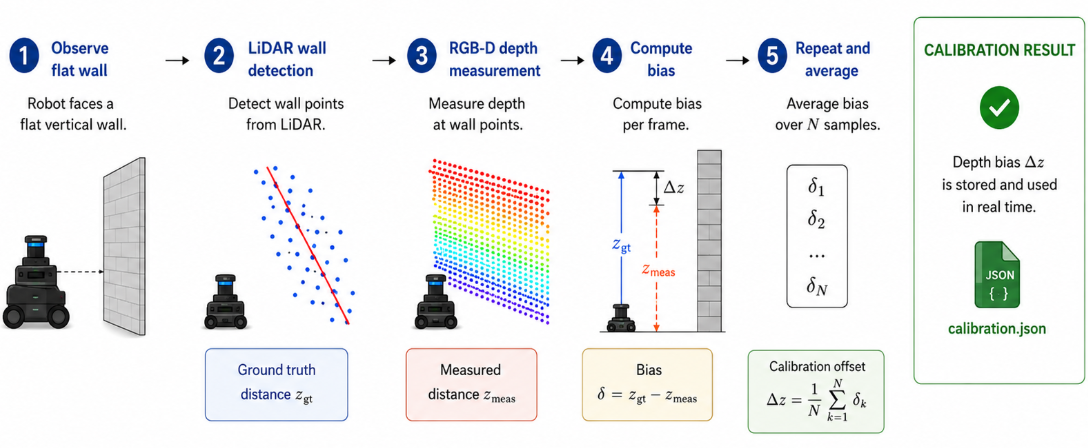
\includegraphics[width=1.0\linewidth]{figures/ch04/depth_correction.png}
    \caption{depth bias correction algorithm}
    \label{fig:depth_correction}
\end{figure}

%---------------------------------------------------------------
\subsubsection{Angular Grid Projection}
%---------------------------------------------------------------

Both sensors are independently projected onto a uniform output angular
grid spanning $[\theta_{\min}, \theta_{\max}]$ with resolution
$\Delta\theta$, yielding

\begin{equation}
    N_{\text{bins}} =
        \left\lfloor
            \frac{\theta_{\max} - \theta_{\min}}{\Delta\theta}
        \right\rfloor
    \label{eq:nbins}
\end{equation}

bins. Each RGBD point that survives the height filter
$z_{\min} \leq z' \leq z_{\max}$ is projected to a bearing and
two-dimensional range,

\begin{equation}
    \theta_{i} = \operatorname{atan2}(y_{i}', x_{i}'),
    \qquad
    \rho_{i} = \sqrt{x_{i}^{\prime\,2} + y_{i}^{\prime\,2}},
    \label{eq:project}
\end{equation}

and assigned to bin $b_{i} = \lfloor(\theta_{i} -
\theta_{\min})/\Delta\theta\rfloor$. The LiDAR scan is re-binned onto
the same grid identically. In both cases the minimum range per bin is
retained, ensuring the closest obstacle in each angular direction is
always reported. Bins receiving no points are set to $+\infty$,
indicating no detection.

%---------------------------------------------------------------
\subsubsection{Range-Adaptive Weighted Fusion}
%---------------------------------------------------------------

With both sensors mapped onto the same grid, fusion is performed
independently per bin. The RGB-D camera's depth uncertainty grows
approximately as $\sigma \propto r^{2}$~\cite{delhibabu2026},
motivating an exponentially decaying confidence weight:

\begin{equation}
    \beta(r) = \exp\!\left(-\frac{r^{2}}{2\,\sigma_{\text{rgbd}}^{2}}\right).
    \label{eq:beta}
\end{equation}

When both sensors detect an obstacle in the same bin, the fused range
is computed as a weighted average,

\begin{equation}
    r_{\text{fused}} =
        \frac{\alpha\,r_{L} + \beta(r_{R})\,r_{R}}{\alpha + \beta(r_{R})},
    \label{eq:fusion}
\end{equation}

where $\alpha$ is the constant LiDAR confidence weight. At short range
$\beta \approx \alpha$ and the two sensors contribute equally; at long
range $\beta \ll \alpha$ and the output approaches $r_{L}$ smoothly.
Table~\ref{tab:fusion_cases} summarises all four per-bin cases.

\begin{table}[H]
\centering
\caption{Per-bin fusion decision rules}
\label{tab:fusion_cases}
\begin{tabular}{llll}
\hline
\textbf{Case} & \textbf{Condition} & \textbf{Output} \\
\hline
LiDAR only
    & $r_{L}{<}\infty$,\; $r_{R}{=}\infty$
    & $r_{L}$ \\
RGBD only (near)
    & $r_{R}{<}\infty$,\; $r_{L}{=}\infty$,\; $r_{R} < r_{\text{trust}}$
    & $r_{R}$ \\
RGBD only (far)
    & $r_{R}{<}\infty$,\; $r_{L}{=}\infty$,\; $r_{R} \geq r_{\text{trust}}$
    & $r_{\max}$ \\
Both valid
    & $r_{L}{<}\infty$,\; $r_{R}{<}\infty$
    & Eq.~\eqref{eq:fusion} \\
Neither
    & $r_{L}{=}\infty$,\; $r_{R}{=}\infty$
    & $r_{\max}$ \\
\hline
\end{tabular}
\end{table}

The RGBD-only far-range case deserves specific mention: a camera return
with no corresponding LiDAR return beyond $r_{\text{trust}} = 2.5$\,m
is more likely to be a spurious detection than a real obstacle, and
accepting it would risk inflating the costmap with phantom readings.
Discarding it is therefore the safer choice for navigation.

%%%%%%%%%%%%%%%%%%%%%%%%%%%%%%%%%%%%%%%%%%%%%%%%%%%%%%%%%%%%%%%%%%%
\subsection{Implementation and Parameters}
%%%%%%%%%%%%%%%%%%%%%%%%%%%%%%%%%%%%%%%%%%%%%%%%%%%%%%%%%%%%%%%%%%%

%---------------------------------------------------------------
\subsubsection{Software Architecture}
%---------------------------------------------------------------

The fusion system comprises two ROS\,2 nodes backed by a shared,
ROS-free utility module (\texttt{fusion\_utils.py}). The
\textit{calibration node} runs once prior to deployment, collects
RANSAC bias samples, and then idles while keeping the latched
\texttt{/depth\_bias} topic live. The \textit{fusion node} runs
continuously throughout operation. Separating the two nodes ensures
that navigation is never blocked by calibration and that all
mathematical algorithms — RANSAC fitting, coordinate transforms,
range-adaptive fusion — can be unit-tested with standard Python
tooling, without instantiating a ROS node or replaying sensor data.

%---------------------------------------------------------------
\subsubsection{Key Design Decisions}
%---------------------------------------------------------------

\paragraph{Temporal synchronization.}
Both sensor streams are paired via \texttt{ApproximateTimeSynchro-\\nizer}
with a 1\,s slop window and per-stream queues of 30 messages,
accommodating the differing publish rates of the LiDAR (10\,Hz) and
RGB-D camera (30\,Hz) without introducing artificial latency.

\paragraph{Depth-bias availability.}
The fusion node initialises $\Delta z$ through a three-tier fallback:
(1)~a \texttt{manual\_delta\_z} launch parameter, if provided;
(2)~\texttt{calibration.json} read from disk at startup, making the
calibrated value available from the first processed frame; and
(3)~$\Delta z = 0$ with a logged warning if neither source is
available. The \texttt{/depth\_bias} subscriber updates $\Delta z$
dynamically at any time using \textsc{Transient\_Local} durability,
so a late-starting fusion node receives the calibration value
immediately upon subscription without requiring re-publication.

\paragraph{Calibration persistence.}
The calibration result is written atomically via a write-then-rename
strategy, ensuring that a power-loss event during the write cannot
corrupt a previously valid file. The stored JSON record includes the
bias value, its standard deviation, and a UTC timestamp for
traceability.

\paragraph{Computational efficiency.}
All array operations are implemented with NumPy vectorization; no
Python-level loops over individual points are used. The per-frame
pipeline — point reading, transformation, height filtering,
projection, re-binning, and fusion — completes in under 10\,ms on
the onboard computer, well within the 33\,ms budget imposed by the
30\,Hz camera rate.

\paragraph{Graceful degradation.}
The fusion node always publishes a scan. If the camera is unavailable,
RGBD bins remain at $+\infty$ and the output is identical to the raw
LiDAR scan. If no calibration data exists, the node runs with
$\Delta z = 0$. Navigation is therefore never blocked by sensor or
calibration failures.

%---------------------------------------------------------------
\subsubsection{System Parameters}
%---------------------------------------------------------------

Table~\ref{tab:topics} lists the ROS\,2 topics exchanged by the
system. Table~\ref{tab:params} lists all tunable parameters with
their default values.

\begin{table}[H]
\centering
\caption{ROS\,2 topic summary}
\label{tab:topics}
\begin{tabular}{lllll}
\hline
\textbf{Topic} & \textbf{Type} & \textbf{Publisher}
               & \textbf{Subscriber} & \textbf{Durability} \\
\hline
\texttt{/realsense/points}
    & PointCloud2   & RealSense driver  & Both nodes       & Volatile \\
\texttt{/scan}
    & LaserScan     & LiDAR driver      & Both nodes       & Volatile \\
\texttt{/depth\_bias}
    & Float32       & Calibration node  & Fusion node      & Transient\_Local \\
\texttt{/calibration\_status}
    & String        & Calibration node  & Dashboard / rqt  & Transient\_Local \\
\texttt{/fused\_scan}
    & LaserScan     & Fusion node       & Nav2 costmap     & Volatile \\
\hline
\end{tabular}
\end{table}

\begin{table}[H]
\centering
\caption{Tunable system parameters}
\label{tab:params}
\begin{tabular}{llll}
\hline
\textbf{Parameter} & \textbf{Default} & \textbf{Unit}
                   & \textbf{Description} \\
\hline
\texttt{calibration\_attempts}  & 10      & —   & Samples averaged for $\Delta z$ \\
\texttt{frontal\_half\_angle\_deg} & 25   & deg & LiDAR arc for wall detection \\
\texttt{min\_height}            & 0.1     & m   & Lower obstacle height bound \\
\texttt{max\_height}            & 2.0     & m   & Upper obstacle height bound \\
\texttt{sigma\_rgbd}            & 1.5     & m   & RGB-D confidence decay constant \\
\texttt{alpha}                  & 1.0     & —   & LiDAR confidence weight \\
\texttt{rgbd\_trust\_max\_range}& 2.5     & m   & Max range for camera-only acceptance \\
\texttt{angle\_increment}       & 0.00581 & rad & Output scan angular resolution \\
\texttt{range\_max}             & 12.0    & m   & Maximum sensor range \\
\texttt{manual\_delta\_z}       & NaN     & m   & Manual bias override (NaN\,=\,use file) \\
\hline
\end{tabular}
\end{table}


\label{sec:odom_imu_fusion}

This section documents the state-estimation pipeline developed to provide continuous, low-drift localization for the Sanad platform. Kinematic dead-reckoning inherently suffers from unbounded drift over time due to mechanical disturbances and wheel slippage. To mitigate this, a multi-stage sensor fusion pipeline was engineered to blend differential-drive wheel odometry with High-rate inertial data. 

The architecture was executed in two structural phases: \textbf{Phase 1} established a custom, single-state scalar Kalman filter implemented from scratch to isolate and validate core recursive operations. Once this mathematical substrate was verified against live streams, the system transitioned to \textbf{Phase 2}, which replaces the prototype with a production-grade Extended Kalman Filter (EKF) utilizing the \texttt{robot\_localization} framework for full planar pose and velocity estimation.

% Requires in the preamble of the parent document:
%   \usepackage{tikz}
%   \usetikzlibrary{positioning, arrows.meta, fit, backgrounds}

% ------------------------------------------------------------------
\subsection{System Architecture and Data Flow}
\label{subsec:architecture}

The subsystem operates as a producer--consumer pipeline across five interoperating nodes. To standardize communications and avoid semantic repetition throughout this chapter, the mapping between underlying software topics and their academic designations is established in Table~\ref{tab:topic_mapping}.

\begin{table}[H]
\centering
\caption{Subsystem Topic and Signal Mapping Identifier}
\label{tab:topic_mapping}
\begin{tabular}{@{}lll@{}}
\toprule
Academic Designation & Technical ROS 2 Topic & Functional Description \\
\midrule
Noisy Odometry Stream & \texttt{/sanad\_controller/odom\_noisy} & Drift-injected kinematic twist and pose \\
Raw Inertial Stream & \texttt{/imu/out} & Unaligned IMU orientation and rates \\
Aligned Inertial Stream & \texttt{/imu\_ekf} & REP-105 frame-corrected IMU data \\
Phase 1 Reference Output & \texttt{/sanad\_controller/odom\_kalman} & Custom 1D scalar yaw-rate estimate \\
Phase 2 Filtered Estimate & \texttt{/odometry/filtered} & Production EKF 15-state output \\
\bottomrule
\end{tabular}
\end{table}

The independent sensing modalities are modified by helper nodes before being handed to the tracking filters, each publishing an independent state estimate. Figure~\ref{fig:dataflow} outlines the topic-level data routing, and Figure~\ref{fig:frametree} details the published coordinate frame hierarchy.

\begin{figure}[H]
\centering
\begin{tikzpicture}[
    node distance=1.5cm and 2.5cm,
    box/.style={draw, rounded corners, align=center, minimum height=1.4cm, minimum width=4.5cm, font=\small, fill=white},
    src/.style={box, fill=blue!5, thick, draw=blue!60!black},
    mid/.style={box, fill=gray!5, thick, draw=gray!60!black},
    est/.style={box, fill=orange!5, thick, draw=orange!70!black},
    out/.style={box, fill=green!5, thick, draw=green!60!black},
    lbl/.style={font=\scriptsize\ttfamily, align=center, fill=white, inner sep=2pt},
    arr/.style={-{Stealth[length=2.5mm]}, thick, rounded corners=4pt}
]

    % --- Row 1: Sources ---
    \node[src] (drive) {Diff-drive controller\\/ Gazebo plugin};
    \node[src, right=2.5cm of drive] (imudrv) {IMU driver /\\filter node};

    % --- Row 2: Intermediaries ---
    \node[mid, below=of drive] (noisyctrl) {\texttt{noisy\_controller}\\(adds Gaussian noise)};
    \node[mid, below=of imudrv] (repub) {\texttt{imu\_republisher.py}\\(overwrites \texttt{frame\_id})};

    % --- Row 3: Estimators (Titles embedded inside the nodes safely) ---
    \node[est, below=2cm of noisyctrl] (kf) {\textbf{Phase 1: Algorithmic Verification}\\\texttt{kalman\_filter}\\(custom 1D, angular.z)};
    \node[est, below=2cm of repub] (ekf) {\textbf{Phase 2: Production Estimator}\\\texttt{ekf\_filter\_node}\\(\texttt{robot\_localization}, 15-state)};

    % --- Row 4: Outputs ---
    \node[out, below=0.8cm of kf] (outkf) {output: \texttt{odom\_kalman}};
    \node[out, below=0.8cm of ekf] (outekf) {output: \texttt{odometry/filtered}};

    % --- Primary Vertical Routing ---
    \draw[arr] (drive) -- node[lbl] {\texttt{joint\_states}} (noisyctrl);
    \draw[arr] (imudrv) -- node[lbl] {\texttt{imu/out}} (repub);
    \draw[arr] (noisyctrl) -- node[lbl] {\texttt{odom\_noisy}} (kf);
    \draw[arr] (repub) -- node[lbl] {\texttt{imu\_ekf}} (ekf);
    \draw[arr] (kf) -- (outkf);
    \draw[arr] (ekf) -- (outekf);

    % --- Cross-Routing (Snaking down the middle channel) ---
    % 1. Noisy odom routing to EKF (Label placed near noisyctrl)
    \draw[arr, draw=blue!70!black] (noisyctrl.east)
        -- ++(1.2, 0) node[lbl, above, pos=0.8] {\texttt{odom\_noisy (vx, vy)}}
        |- (ekf.165);

    % 2. Raw IMU routing to Phase 1 KF (Label placed near imudrv)
    \draw[arr, draw=red!70!black] (imudrv.west)
        -- ++(-1.2, 0) node[lbl, above, pos=0.8] {\texttt{imu/out}}
        |- (kf.15);

\end{tikzpicture}
\caption{Subsystem block architecture and signal routing map.}
\label{fig:dataflow}
\end{figure}

\begin{figure}[H]
\centering
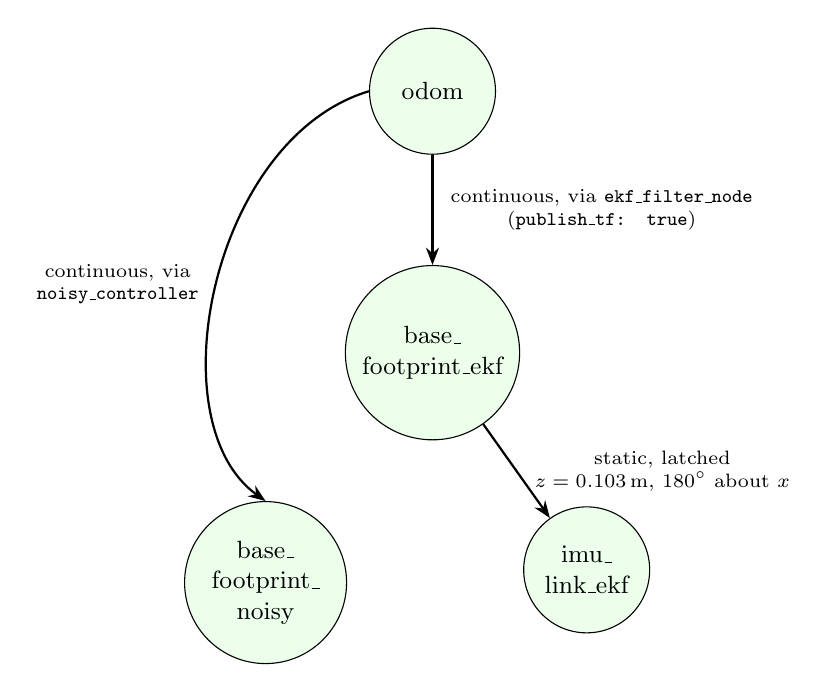
\begin{tikzpicture}[
    node distance=14mm,
    frame/.style={draw, circle, minimum size=1.6cm, align=center, font=\small, fill=green!8},
    arr/.style={-{Stealth[length=2.2mm]}, thick},
    lbl/.style={font=\scriptsize, align=center}
]
    \node[frame] (odom) {odom};
    \node[frame, below=of odom] (bfekf) {base\_\\footprint\_ekf};
    \node[frame, below left=14mm and 6mm of bfekf] (bfnoisy) {base\_\\footprint\_\\noisy};
    \node[frame, below right=14mm and 6mm of bfekf] (imulink) {imu\_\\link\_ekf};

    \draw[arr] (odom) -- (bfekf) node[lbl, midway, right=1mm]
        {continuous, via \texttt{ekf\_filter\_node}\\(\texttt{publish\_tf: true})};
    \draw[arr] (odom.west) .. controls +(-20mm,-6mm) and +(-14mm,10mm) .. (bfnoisy.north)
        node[lbl, pos=0.5, left=1mm] {continuous, via\\\texttt{noisy\_controller}};
    \draw[arr] (bfekf) -- (imulink) node[lbl, midway, right=1mm]
        {static, latched\\$z=0.103$\,m, $180^\circ$ about $x$};
\end{tikzpicture}
\caption{Subsystem coordinate transformation tree configuration.}
\label{fig:frametree}
\end{figure}

The \texttt{base\_footprint\_ekf} frame is shared as both the child frame for the noisy controller and the tracking target for the EKF, eliminating intermediate coordinate translation overhead. Additionally, Phase 1 was deliberately retained alongside Phase 2. Because the EKF operates independently of the scalar filter, the Phase 1 pipeline functions as an un-isolated structural reference to validate the convergence behavior and parameter tuning of the complete Phase 2 EKF without interfering with the primary navigation path.

% ------------------------------------------------------------------
\subsection{Kinematic Modeling and Noise Simulation}
\label{subsec:kinematics}

\subsubsection{Differential-drive forward kinematics}

The kinematic tracking node processes left and right wheel angular positions ($p_L, p_R$) reported via joint states to integrate linear and angular changes. Given wheel radius $R$ and separation distance $L$, wheel angular velocities over control step $\Delta t$ are derived via:
\begin{equation}
\dot{\varphi}_L = \frac{\Delta p_L}{\Delta t}, \qquad
\dot{\varphi}_R = \frac{\Delta p_R}{\Delta t},
\label{eq:wheel_vel}
\end{equation}
yielding the current body-frame linear ($v$) and angular ($\omega$) twist components:
\begin{equation}
v = \frac{R\,\dot{\varphi}_R + R\,\dot{\varphi}_L}{2}, \qquad
\omega = \frac{R\,\dot{\varphi}_L - R\,\dot{\varphi}_R}{L}.
\label{eq:twist}
\end{equation}

Discrete spatial integration maps the structural arc increment $d_s$ and heading update $d\theta$ directly from instantaneous wheel displacements:
\begin{equation}
d_s = \frac{R\,\Delta p_R + R\,\Delta p_L}{2}, \qquad
d\theta = \frac{R\,\Delta p_R - R\,\Delta p_L}{L}.
\label{eq:increments}
\end{equation}
The discrete planar pose is then advanced using a first-order Euler integration step:
\begin{align}
\theta_k &= \theta_{k-1} + d\theta, \label{eq:theta_update}\\
x_k &= x_{k-1} + d_s \cos(\theta_k), \label{eq:x_update}\\
y_k &= y_{k-1} + d_s \sin(\theta_k). \label{eq:y_update}
\end{align}

The implementation uses different sign conventions for angular velocity and heading integration. Although internally self-consistent, future versions should unify these conventions to streamline downstream debugging.

\subsubsection{Encoder noise injection}

To evaluate filter resilience under non-ideal operating conditions, zero-mean Gaussian noise is added to the ideal wheel position profiles prior to velocity calculation:
\begin{equation}
\tilde{p}_L = p_L + \epsilon_L, \qquad \tilde{p}_R = p_R + \epsilon_R,
\qquad \epsilon_L, \epsilon_R \sim \mathcal{N}(0, \sigma^2),
\end{equation}
where $\sigma = 0.005$\,rad. This introduces localized stochastic disturbance to simulate encoder discretization and mechanical play. Furthermore, launch-time calibration scaling introduces deterministic parameter offsets (\texttt{wheel\_radius\_error} and \texttt{wheel\_separation\_error}) to test filter resilience against real-world mechanical scale variations.

% ------------------------------------------------------------------
\subsection{Phase 1: Algorithmic Verification --- The Custom 1D Kalman Filter}
\label{subsec:kf_theory}

To isolate the estimation mechanics from multi-dimensional mathematical overhead, Phase 1 establishes an independent, scalar (1D) filter tracking a single state: yaw rate ($\omega$). This programmatic reduction allowed direct validation of prediction, update, and noise bounds against the live streaming sensor buses. 

\subsubsection{State prediction}

The filter projects the state estimate $\hat{x}$ and inflates the associated estimation variance $P$ using the control step input $u_k$ derived from the noisy odometry stream and process noise covariance $Q$:
\begin{align}
\hat{x}_{k|k-1} &= \hat{x}_{k-1|k-1} + u_k, \label{eq:kf_predict_mean}\\
P_{k|k-1} &= P_{k-1|k-1} + Q. \label{eq:kf_predict_var}
\end{align}

\subsubsection{Measurement update}

When an updated angular measurement $z_k$ arrives via the raw inertial stream, the state and variance updates are handled through a direct covariance-weighted combination using measurement noise covariance $R$:
\begin{align}
\hat{x}_{k|k} &= \frac{R\,\hat{x}_{k|k-1} + P_{k|k-1}\,z_k}{P_{k|k-1} + R}, \label{eq:kf_update_mean}\\
P_{k|k} &= \frac{P_{k|k-1}\,R}{P_{k|k-1} + R}. \label{eq:kf_update_var}
\end{align}
This implementation map resolves as algebraically identical to the classical textbook innovation format:
\begin{align}
\hat{x}_{k|k} &= \hat{x}_{k|k-1} + K_k\left(z_k - \hat{x}_{k|k-1}\right), \\
P_{k|k} &= (1 - K_k)\,P_{k|k-1},
\end{align}
where the intermediate Kalman gain is defined as $K_k = P_{k|k-1} / (P_{k|k-1} + R)$. Verification tests confirmed that this core recursion stabilized bounded variations reliably, demonstrating algorithmic readiness prior to expanding the state scope in Phase 2.

% ------------------------------------------------------------------
\subsection{Phase 2: Full State Estimation --- The Extended Kalman Filter}
\label{subsec:ekf}

Phase 2 replaces the single-state test structure with a multi-dimensional \texttt{ekf\_node} from the \texttt{robot\_localization} framework to fulfill the spatial pose dependencies of the Nav2 planning stack. The internal estimation tracks a standard 15-element kinematic state vector:
\begin{equation}
\mathbf{x} = \begin{bmatrix} x & y & z & \phi & \theta & \psi &
\dot{x} & \dot{y} & \dot{z} & \dot{\phi} & \dot{\theta} & \dot{\psi} &
\ddot{x} & \ddot{y} & \ddot{z} \end{bmatrix}^\top.
\end{equation}
Planar stability is maintained by setting \texttt{two\_d\_mode: true}, which suppresses vertical drift corrections.

\subsubsection{Configuration vector selection}

Boolean observation masks isolate specific trusted signal components from each tracking sensor inside \texttt{ekf.yaml}:
\begin{itemize}
\item \textbf{Odometry Configuration:} Only body-frame linear velocity fields ($\dot{x}, \dot{y}$) are enabled. Absolute position integration is explicitly omitted to prevent the filter from feedback-amplifying the dead-reckoning position drift tracking inside the kinematic source node.
\item \textbf{Inertial Configuration:} Absolute heading orientation ($\psi$), rotational velocity ($\dot{\psi}$), and linear forward acceleration ($\ddot{x}$) are explicitly mapped to drive orientation tracking.
\end{itemize}

Additionally, the configuration operates with both odometry and inertial inputs configured in differential mode. This numerical differencing converts raw absolute observations into relative updates between consecutive steps, removing constant sensor bias offsets from driving long-term state divergence.

\subsubsection{Frame alignment and REP-105 compliance}

To integrate cleanly with ROS-standard coordinate conventions, the architecture leverages two auxiliary alignment nodes:
\begin{itemize}
\item \textbf{Static Transform Node:} Manages physical mounting offset errors by locking the coordinate link from \texttt{base\_footprint\_ekf} to \texttt{imu\_link\_ekf} ($z = 0.103$\,m with a $180^\circ$ inversion about the $x$-axis).
\item \textbf{Inertial Relay Node:} Intercepts the raw inertial stream, re-keys its internal metadata frame identifiers to resolve against \texttt{base\_footprint\_ekf}, and publishes the aligned inertial stream to meet the EKF configuration parameters.
\end{itemize}

% ------------------------------------------------------------------
\subsection{System Verification and Diagnostic Methodology}
\label{subsec:verification}

Validation of the fusion layer was conducted systematically across three distinct criteria to evaluate stability before downstream navigation deployment.

\paragraph{Covariance Bounding Analysis}
Upon initialization, state covariance parameters start with high, uncalibrated uncertainty bounds. As continuous sensor frames arrive via the noisy odometry and aligned inertial streams, the covariance fields on the filtered state output must decay monotonically toward a stable, narrow steady-state value. Failure to collapse or stabilize indicates process noise matrix misconfiguration inside \texttt{ekf.yaml}.

\paragraph{High-Frequency Smoothing and Jitter Suppression}
The tracking fidelity was evaluated by comparing the filtered tracking stream against the raw noisy stream in a standardized 3D visualizer. The fusion layer demonstrates appropriate noise attenuation if it strips away high-frequency encoder jitter and rapid acceleration artifacts while simultaneously tracking true physical trajectory trends without introducing significant phase lag.

\paragraph{Cross-Filter Reference Validation}
As established in Section~\ref{subsec:architecture}, the Phase 1 tracking loop remains active alongside Phase 2 for runtime structural diagnostics. Because both estimators stem from the same validated mathematical baseline, plotting the yaw-rate channel of the Phase 1 reference output against the corresponding state estimation of the Phase 2 filtered output provides an absolute metric of filter health. Persistent divergence between the two signals isolates EKF matrix configuration errors or masking mismatches directly, providing an algorithmic sanity check prior to physical hardware testing.

\subsection{Experimental Results and System Validation}
\label{subsec:results}

To quantify the performance of the sensor fusion architecture, the system was evaluated across both dynamic and stationary operating regimes. The analysis isolates the two primary objectives of the subsystem: high-frequency noise suppression (via the Phase 1 scalar filter) and long-term spatial drift correction (via the Phase 2 EKF).

\subsubsection{Angular Velocity Noise Attenuation}

The first evaluation targeted the filter's ability to extract the true angular velocity ($\dot{\psi}$) from the heavily corrupted noisy odometry stream. Figure~\ref{fig:angular_velocity_filtering} illustrates the tracking performance captured via PlotJuggler during two distinct operational states: a static/linear translation phase and a dynamic rotation phase.

\begin{figure}[htpb]
\centering
% Adjust width as needed for your specific page margins
\begin{minipage}{0.48\textwidth}
\centering
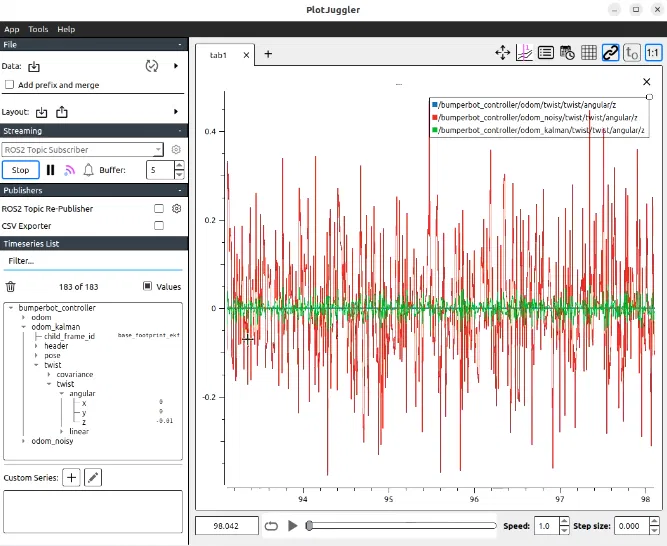
\includegraphics[width=\linewidth]{figures/ch04/stationary_plot.png} % Replace with image_0c5db5.png path
\caption*{ (a) Stationary / Linear Motion }
\end{minipage}\hfill
\begin{minipage}{0.48\textwidth}
\centering
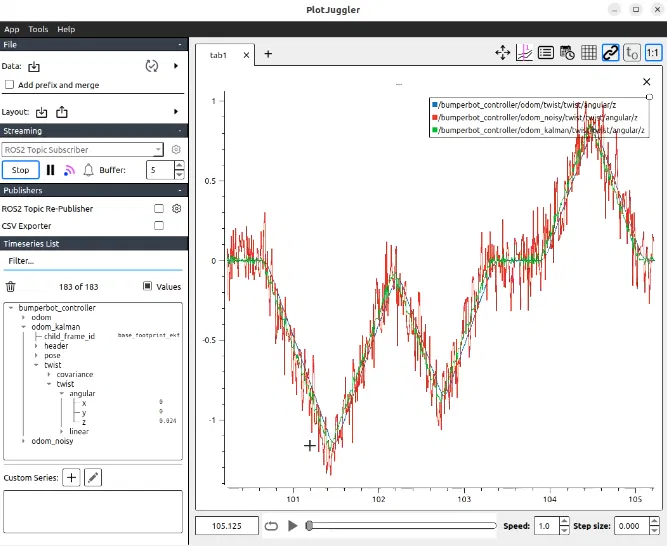
\includegraphics[width=\linewidth]{figures/ch04/rotation_plot.png} % Replace with image_0c5daf.png path
\caption*{ (b) Dynamic Rotation }
\end{minipage}
\caption{Comparative analysis of the $z$-axis angular velocity. The ideal ground-truth signal (blue) is overlaid with the drift-injected noisy stream (red) and the Phase 1 filtered estimate (green). In both the stationary regime (a) and the rotational tracking regime (b), the filtered estimate successfully rejects the high-frequency Gaussian injection while maintaining strict phase alignment with the true motion profile.}
\label{fig:angular_velocity_filtering}
\end{figure}

During stationary or strictly linear motion (Figure~\ref{fig:angular_velocity_filtering}a), the raw encoder noise introduces significant artificial rotational jitter (red trace) which, if left uncorrected, would cause downstream local planners to oscillate erratically. The filtered estimate (green trace) maintains a tightly bounded profile around zero, effectively rejecting the artificial noise.
When subjected to dynamic rotation (Figure~\ref{fig:angular_velocity_filtering}b), the filtered signal successfully tracks the underlying sinusoidal profile of the true odometry without introducing significant phase lag. The continuous overlap of the filtered output with the ideal ground-truth demonstrates that the process and measurement noise matrices ($Q$ and $R$) were tuned correctly, preventing the estimator from becoming sluggish or overly reactive.
\subsubsection{Spatial Drift Correction}

While Phase 1 validated the frequency-domain smoothing, Phase 2 was evaluated on its ability to correct spatial dead-reckoning drift. Figure~\ref{fig:tf_drift} visualizes the localized coordinate frame transformations published during a continuous navigation run.

\begin{figure}[htpb]
\centering
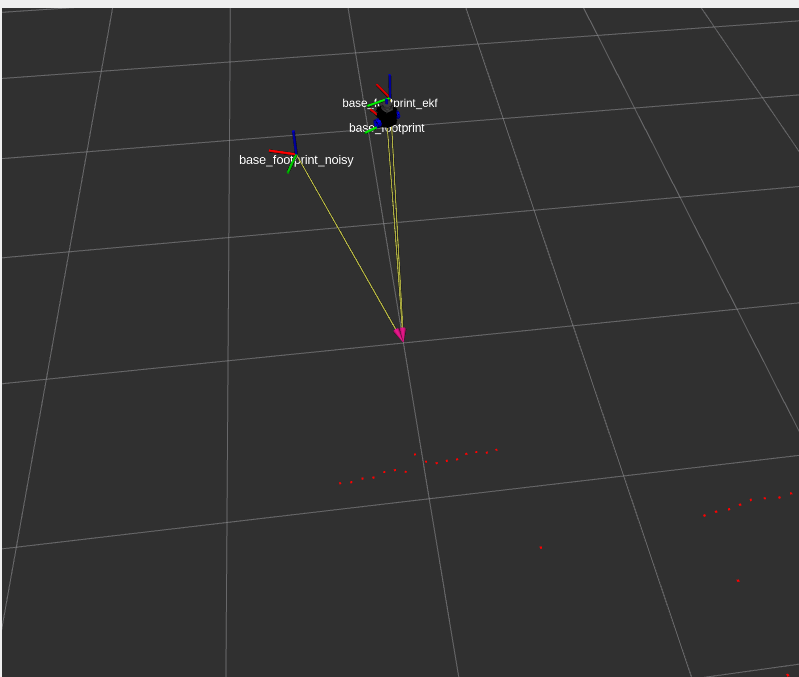
\includegraphics[width=0.7\textwidth]{figures/ch04/tf_drift.png} % Replace with image_0c61ef.png path
\caption{RViz2 visualization of the coordinate frame hierarchy after continuous operation. The filtered \texttt{base\_footprint\_ekf} frame maintains strong geometric alignment with the ground-truth \texttt{base\_footprint}, whereas the uncorrected \texttt{base\_footprint\_noisy} frame has drifted significantly from the true platform position.}
\label{fig:tf_drift}
\end{figure}

Because the noisy odometry stream integrates its position open-loop from corrupted twist velocities, the \texttt{\detokenize{base_footprint_noisy}} frame exhibits severe accumulated drift, physically diverging from the true robot center over time. By incorporating the absolute heading and rate corrections from the aligned inertial stream, the Phase 2 EKF suppresses this divergence. As shown in the visualization, the resulting \texttt{\detokenize{base_footprint_ekf}} frame remains tightly coupled to the ideal \texttt{\detokenize{base_footprint}}. This geometric alignment confirms that the Phase 2 estimator provides a reliable, drift-resistant spatial reference, satisfying the prerequisites for autonomous path planning and Nav2 deployment.











\FloatBarrier
\section{Block 4: Localization \& Mapping (SLAM \& AMCL)}
Once a reliable odometry base is established, the robot executes mapping and localization within the home.

\begin{itemize}
    \item \textbf{Mapping (SLAM Toolbox)}: During installation, the robot builds a static 2D occupancy grid map of the house at a resolution of $0.05$ meters. It fuses the merged scan topic \texttt{/scan} with the EKF pose. The solver utilizes the Ceres optimizer (\texttt{solver\_plugins::CeresSolver}) and Ceres Linear Solver (\texttt{SPARSE\_NORMAL\_CHOLESKY}) to solve the scan-matching problem.
    \item \textbf{Localization (AMCL)}: During operation, Adaptive Monte Carlo Localization (\texttt{nav2\_amcl}) tracks the robot's pose against the static map. AMCL uses a particle filter, configuring between $500$ and $2000$ particles. The particles are updated when the robot rotates by more than $0.2$ radians or moves by $0.25$ meters.
\end{itemize}

\begin{figure}[H]
\centering
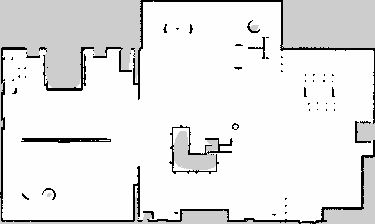
\includegraphics[width=0.6\textwidth]{figures/ch04/slam_map.png}
\caption{2D occupancy grid map of the home generated by SLAM Toolbox.}
\label{fig:slam_map}
\end{figure}

\begin{figure}[H]
    \centering
    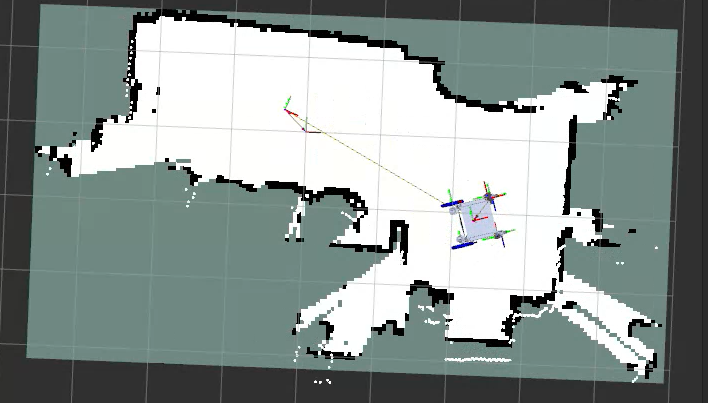
\includegraphics[width=0.6\textwidth]{figures/ch04/real_slam_mapping.png}
    \caption{Real-world map creation using SLAM Toolbox during initial system calibration.}
    \label{fig:real_map_creation}
\end{figure}

\subsection{SLAM Toolbox Parameters}
Table~\ref{tab:slam_params} summarizes the key configuration parameters used for the mapping process.

\begin{table}[H]
\centering
\caption{SLAM Toolbox key parameters.}
\label{tab:slam_params}
\begin{tabular}{ll}
\toprule
\textbf{Parameter} & \textbf{Value} \\
\midrule
Mode & \texttt{mapping} \\
Resolution & $0.05$ m \\
Max laser range & $12.0$ m \\
Minimum travel distance & $0.5$ m \\
Minimum travel heading & $0.5$ rad \\
Solver plugin & \texttt{solver\_plugins::CeresSolver} \\
Ceres linear solver & \texttt{SPARSE\_NORMAL\_CHOLESKY} \\
Ceres preconditioner & \texttt{SCHUR\_JACOBI} \\
Loop closure search & Enabled \\
Scan topic & \texttt{/scan} \\
\bottomrule
\end{tabular}
\end{table}

\subsection{AMCL Parameters}
Table~\ref{tab:amcl_params} lists the AMCL particle filter parameters used during localization.

\begin{table}[H]
\centering
\caption{AMCL key parameters.}
\label{tab:amcl_params}
\begin{tabular}{ll}
\toprule
\textbf{Parameter} & \textbf{Value} \\
\midrule
Minimum particles & $500$ \\
Maximum particles & $2000$ \\
Update min distance & $0.25$ m \\
Update min angle & $0.2$ rad \\
Resample interval & $1$ \\
Transform tolerance & $1.0$ s \\
Laser model type & \texttt{likelihood\_field} \\
Odometry model type & \texttt{diff} \\
Alpha1--Alpha5 (odom noise) & $0.2$ (default) \\
Recovery alpha slow & $0.001$ \\
Recovery alpha fast & $0.1$ \\
\bottomrule
\end{tabular}
\end{table}

\subsection{Particle Filter Convergence}
Figure~\ref{fig:amcl_lost} shows the particle distribution shortly after initialization, when the robot's pose is highly uncertain and particles are spread broadly across the map. Figure~\ref{fig:amcl_converged} shows the particle cloud after convergence, once the robot has localized correctly and the particles have collapsed tightly around the true pose.

\begin{figure}[H]
\centering

\begin{minipage}{0.48\textwidth}
    \centering
    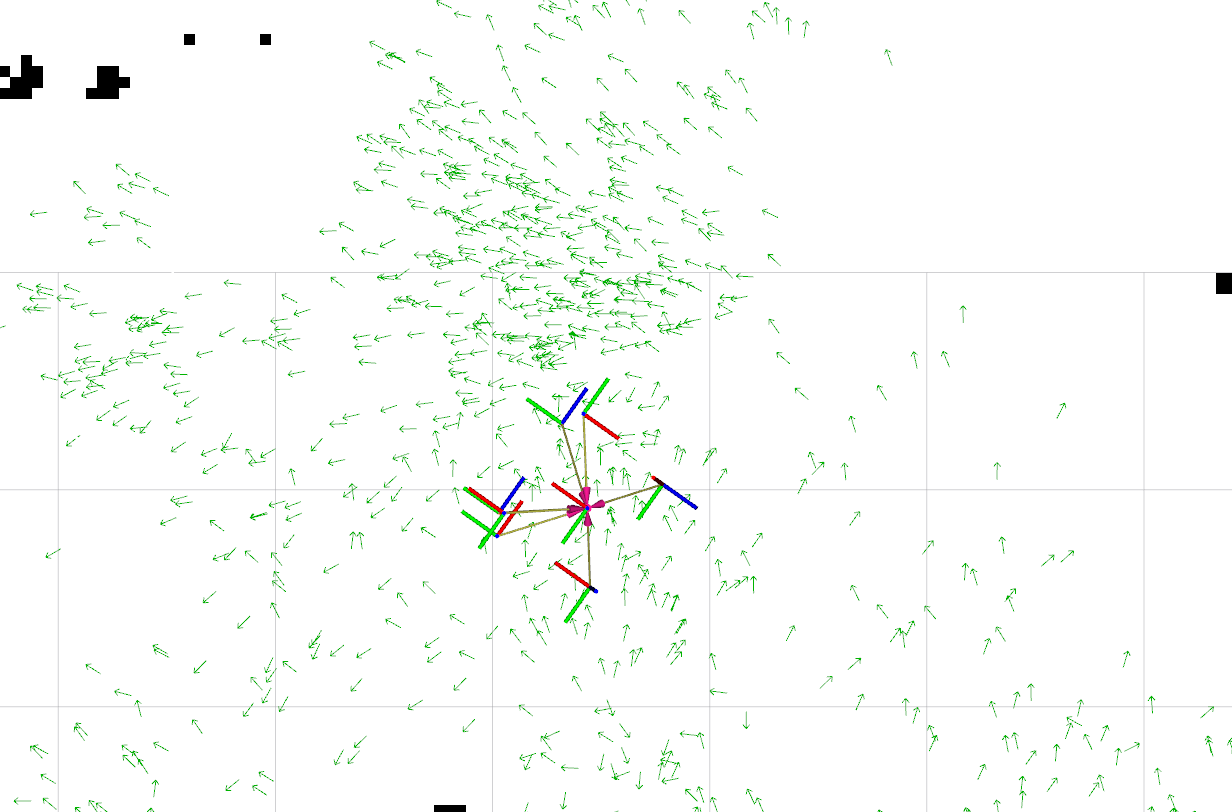
\includegraphics[width=\linewidth]{figures/ch04/lost_robot.png}
    \caption{Dispersed particle cloud indicating high pose uncertainty (robot not yet localized).}
    \label{fig:amcl_lost}
\end{minipage}
\hfill
\begin{minipage}{0.48\textwidth}
    \centering
    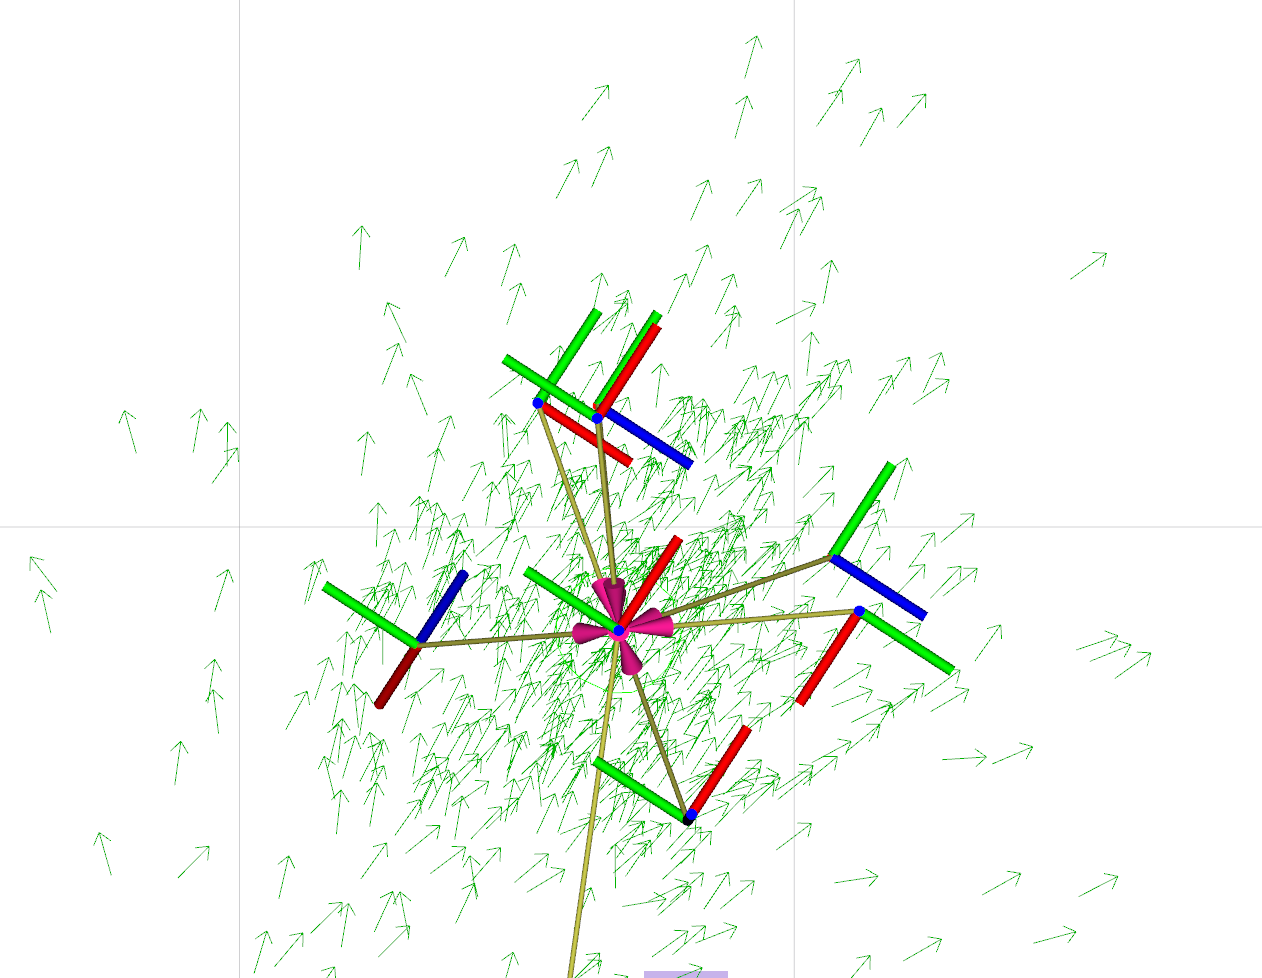
\includegraphics[width=\linewidth]{figures/ch04/localized_robot.png}
    \caption{Converged particle cloud indicating accurate localization at the true robot pose.}
    \label{fig:amcl_converged}
\end{minipage}

\end{figure}

\section{Block 5: Global Path Planning}
\label{sec:planner}
% ─────────────────────────────────────────────────────────────────────────────

\subsection*{Architecture --- Behaviour Tree Navigator}

All high-level navigation requests (``go to the kitchen'', ``follow the caregiver'') are managed by the \texttt{bt\_navigator} node, which drives a Nav2 Behaviour Tree. The BT orchestrates the sequence: \emph{localise} $\to$ \emph{plan} $\to$ \emph{control} $\to$ \emph{recover}, and retries or escalates to recovery behaviours when any sub-task fails. Key BT-Navigator parameters from \texttt{bt\_navigator.yaml}:
\begin{itemize}\itemsep=2pt
    \item \texttt{global\_frame}: \texttt{map} --- all goal poses are expressed in the AMCL map frame.
    \item \texttt{odom\_topic}: \texttt{/sanad\_controller/odom} --- BT monitors this topic to compute progress.
    \item \texttt{transform\_tolerance}: $0.3$~s --- maximum age of a valid TF lookup inside the BT.
    \item \texttt{bt\_loop\_duration}: $10$~ms --- the BT ticks at 100~Hz, ensuring rapid replanning.
    \item \texttt{default\_server\_timeout}: $1000$~ms --- action servers must respond within 1~second before the BT marks them as failed.
\end{itemize}

\subsection*{Global Costmap}

Before the planner can run, it needs a model of the world that encodes both static structure (walls, furniture) and live obstacle data. The global costmap is built from three stacked plugins, configured in \texttt{planner\_server.yaml}:

\begin{enumerate}
    \item \textbf{StaticLayer} (\texttt{nav2\_costmap\_2d::}\allowbreak\texttt{StaticLayer}): loads the pre-built occupancy grid from the \texttt{/map} topic (the SLAM-generated \texttt{.pgm} file). Subscribed with \texttt{map\_subscribe\_}\allowbreak\texttt{transient\_local:}\allowbreak\texttt{true} to guarantee the map is received even if it was published before the costmap node started.
    \item \textbf{ObstacleLayer} (\texttt{nav2\_costmap\_2d::}\allowbreak\texttt{ObstacleLayer}): marks and clears cells in real time using the merged laser scan \texttt{/scan}. Obstacle marking range is limited to $2.5$~m; raytrace clearing extends to $3.0$~m, so that cells behind a removed obstacle are cleared promptly. Both \texttt{marking} and \texttt{clearing} are enabled.
    \item \textbf{InflationLayer} (\texttt{nav2\_costmap\_2d::}\allowbreak\texttt{InflationLayer}): wraps every occupied cell with a cost gradient (inflation radius $0.65$~m, scaling factor $k=3.0$). The mathematical basis and design rationale for these values are discussed in Section~\ref{sec:costmap}.
\end{enumerate}

The global costmap uses a $0.05$~m/cell resolution, matching the SLAM map resolution, and updates at $1.0$~Hz (adequate for static environments, where the map changes slowly). The robot footprint is modelled as a circle with radius $0.2$~m. The configuration parameters are detailed in Table~\ref{tab:planner_yaml}.

\subsection*{Smac Planner 2D --- Search Algorithm}

The planner plugin registered under the alias \texttt{GridBased} is \texttt{nav2\_smac\_planner/SmacPlanner2D}. It runs a graph-search over the discrete costmap grid and finds the minimum-cost path from the robot's current cell to the goal cell. Table~\ref{tab:planner_yaml} lists the primary planner and global costmap configuration parameters.

\begin{table}[H]
\centering
\caption{Smac Planner 2D and global costmap configuration parameters (\texttt{planner\_server.yaml}).}
\label{tab:planner_yaml}
\renewcommand{\arraystretch}{1.2}
\begin{tabular}{lll}
\toprule
\textbf{Component} & \textbf{Parameter} & \textbf{Value} \\
\midrule
\multirow{6}{*}{\textbf{Smac Planner}} 
 & \texttt{plugin} & \texttt{SmacPlanner2D} \\
 & \texttt{tolerance} & $0.125$~m \\
 & \texttt{allow\_unknown} & \texttt{true} \\
 & \texttt{max\_planning\_time} & $2.0$~s \\
 & \texttt{cost\_travel\_multiplier} & $2.0$ \\
 & \texttt{smoother.w\_smooth / w\_data} & $0.3$ / $0.2$ \\
\midrule
\multirow{8}{*}{\textbf{Global Costmap}}
 & \texttt{global\_frame} & \texttt{map} \\
 & \texttt{update\_frequency} & $1.0$~Hz \\
 & \texttt{resolution} & $0.05$~m/cell \\
 & \texttt{robot\_radius} & $0.20$~m \\
 & \texttt{plugins} & Static, Obstacle, Inflation \\
 & \texttt{obstacle\_layer.max\_range} & $2.5$~m \\
 & \texttt{inflation\_layer.radius} & $0.65$~m \\
 & \texttt{inflation\_layer.cost\_scaling} & $3.0$ \\
\bottomrule
\end{tabular}
\end{table}

\paragraph{Key parameter choices explained.}
\begin{itemize}\itemsep=2pt
    \item \textbf{\texttt{allow\_unknown: true}}: In domestic environments, parts of the map may not have been fully explored (e.g.\ inside a wardrobe or under furniture). Setting this to \texttt{true} allows the planner to route through unknown cells rather than refusing to plan; the obstacle layer will clear or mark those cells once the robot approaches and the LiDAR covers them.
    \item \textbf{\texttt{cost\_travel\_multiplier: 2.0}}: A value of $1.0$ would treat all free cells equally (pure A*); a value greater than $1.0$ makes the planner actively prefer cells far from obstacles, centering the wheelchair in corridors. The value $2.0$ was found empirically to balance path directness and safety margin.
    \item \textbf{\texttt{max\_planning\_time: 2.0}~s}: Prevents a pathological costmap (e.g.\ from a noisy scan burst) from blocking the navigation stack for more than 2~seconds.
\end{itemize}

\begin{figure}[H]
\centering
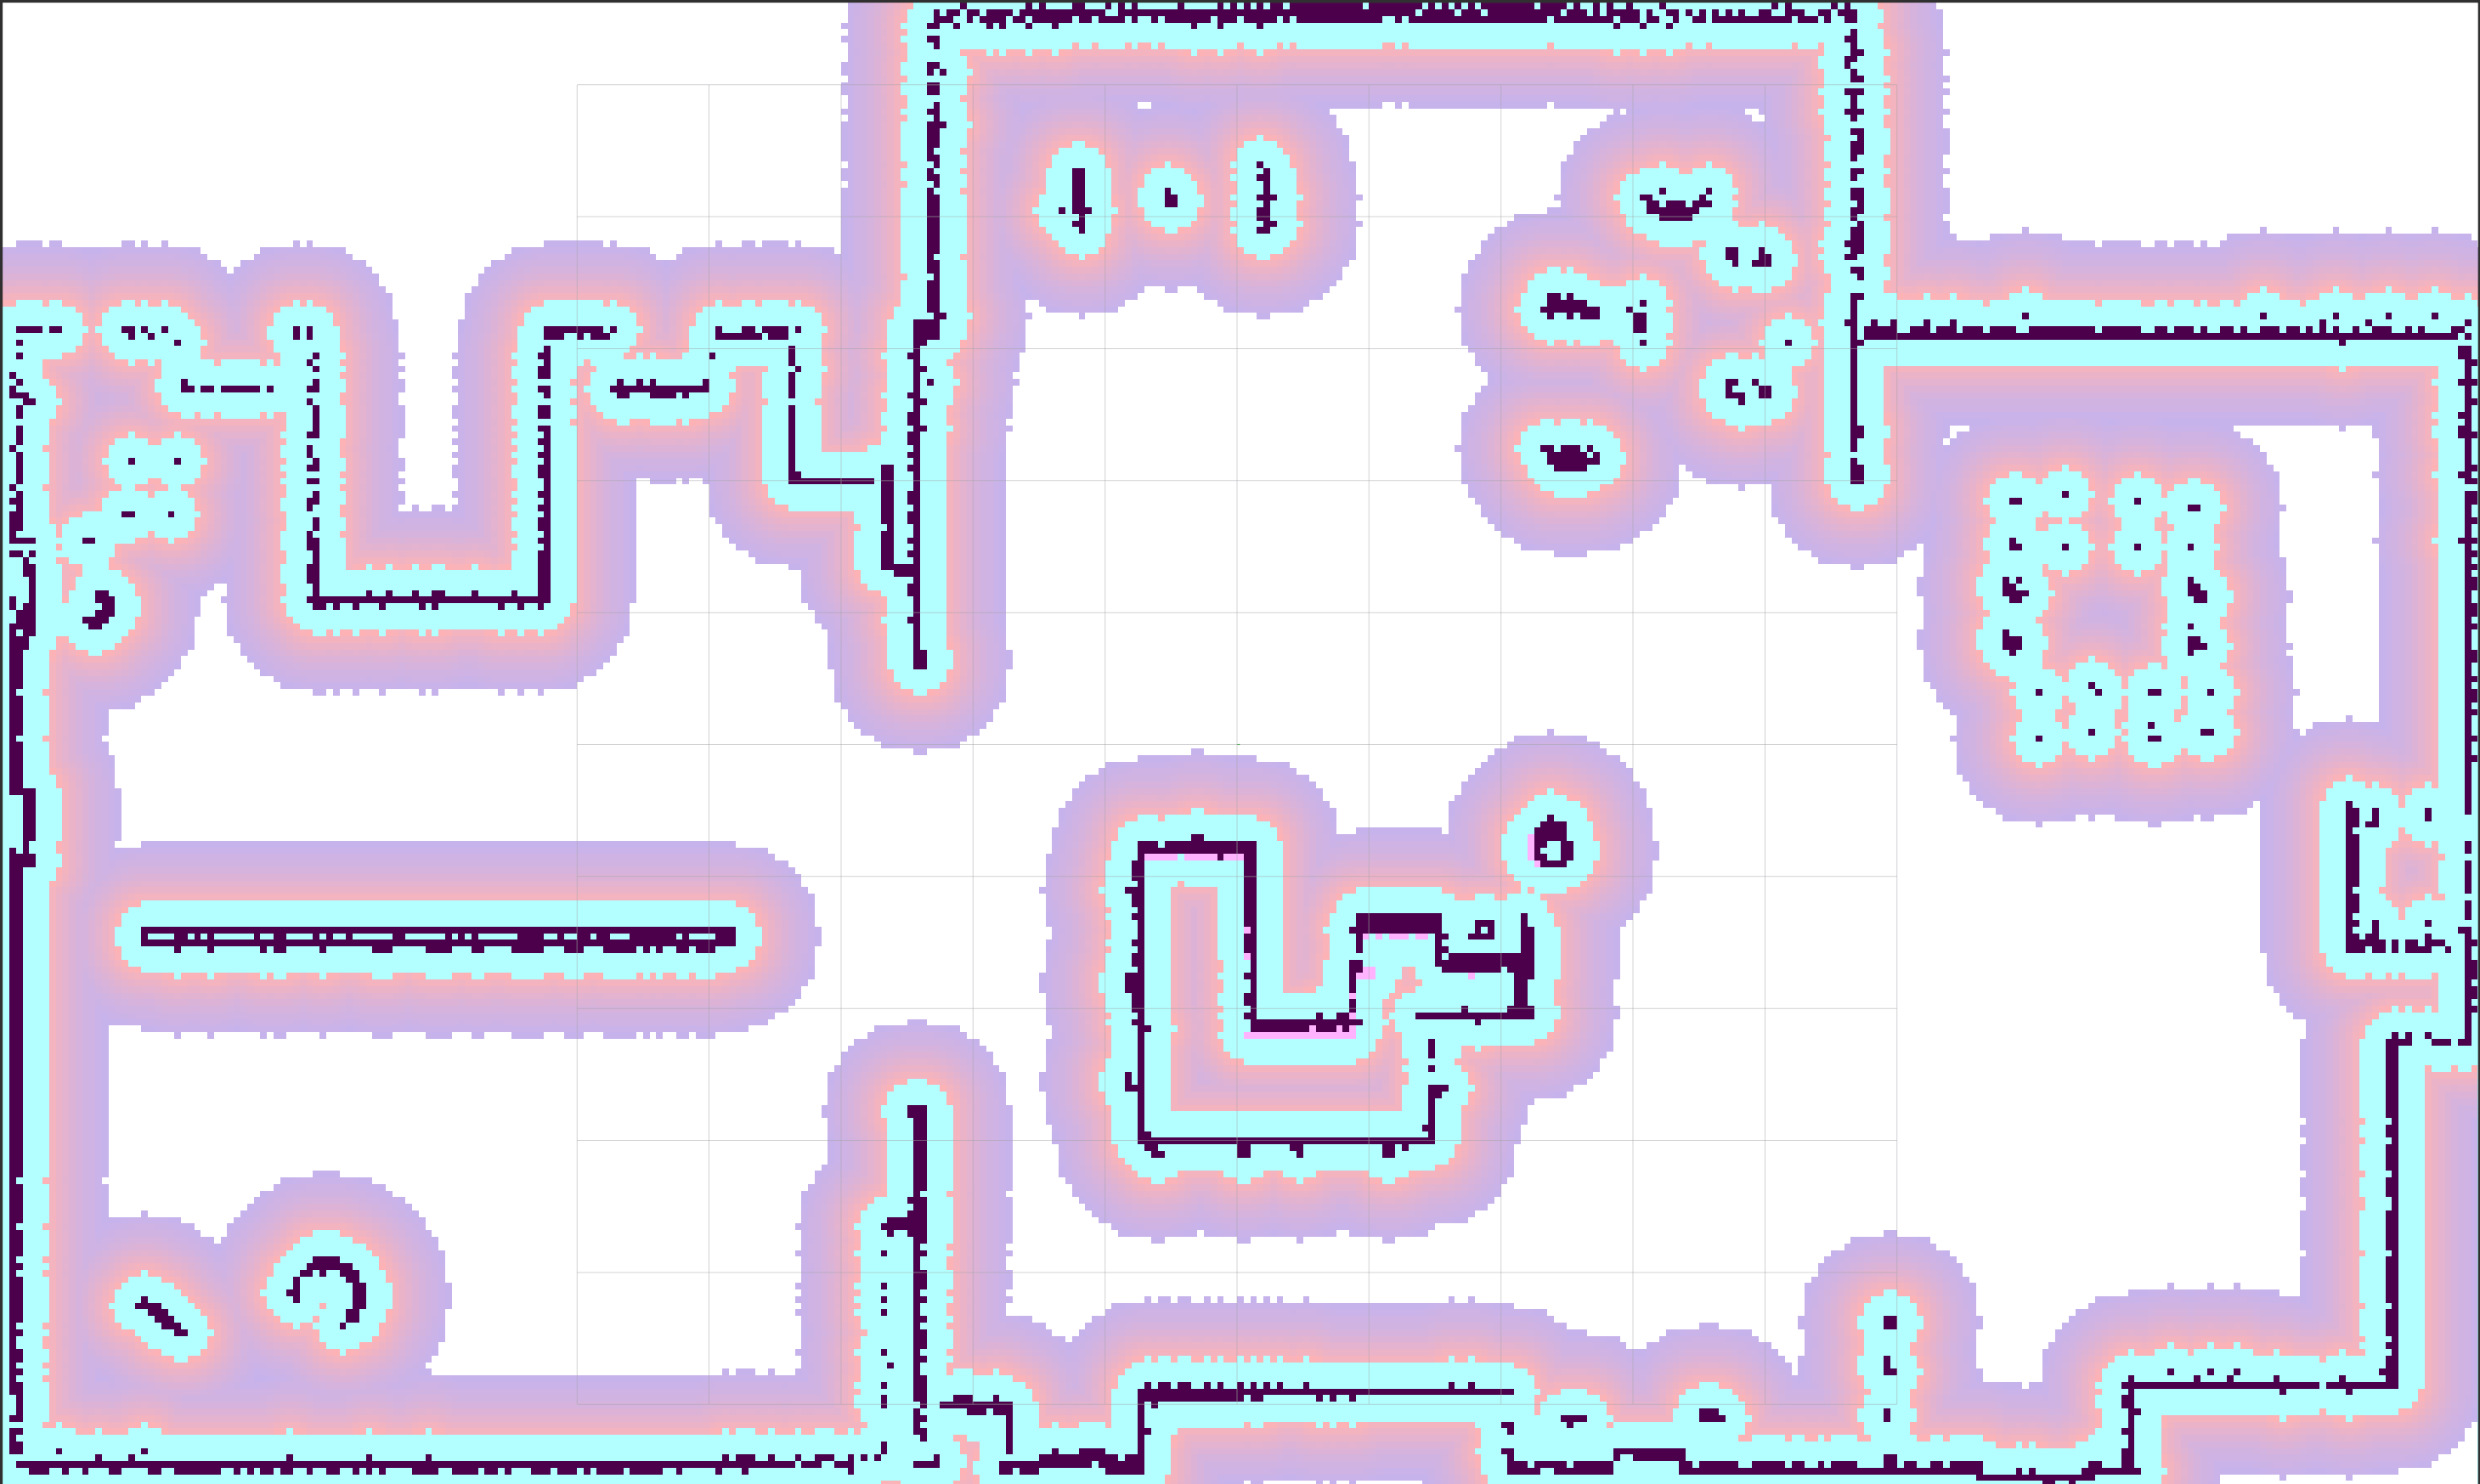
\includegraphics[width=0.85\textwidth]{figures/ch04/global_costmap.png}
\caption{Global costmap overlaid on the occupancy grid map of the home environment. Lethal cells (occupied walls and obstacles) are surrounded by the inflation gradient produced by the InflationLayer, steering the planner away from obstacles and centering paths in open corridors.}
\label{fig:global_costmap_map}
\end{figure}

\subsection*{Path Smoothing}

The raw A* path consists of straight-line segments between grid-cell centres, producing sharp angular waypoints that would force the Pure Pursuit controller to make abrupt heading corrections. Two smoothing stages are applied:

\begin{enumerate}
    \item \textbf{Inline Smac smoother}: embedded inside the planner, this iterative gradient-descent smoother runs for up to $1000$ iterations with a smoothness weight of $w_s = 0.3$ and a data (fidelity) weight of $w_d = 0.2$. It converges when the change in path cost falls below $10^{-10}$.
    \item \textbf{Smoother Server} (\texttt{nav2\_smoother::SimpleSmoother}): an additional downstream smoother node configured in \texttt{smoother\_server.yaml} with \texttt{do\_refinement: true}, which runs a second pass for geometric refinement after the planner hands off the path, further rounding the trajectory before the controller consumes it.
\end{enumerate}
\begin{figure}[H]
    \centering
    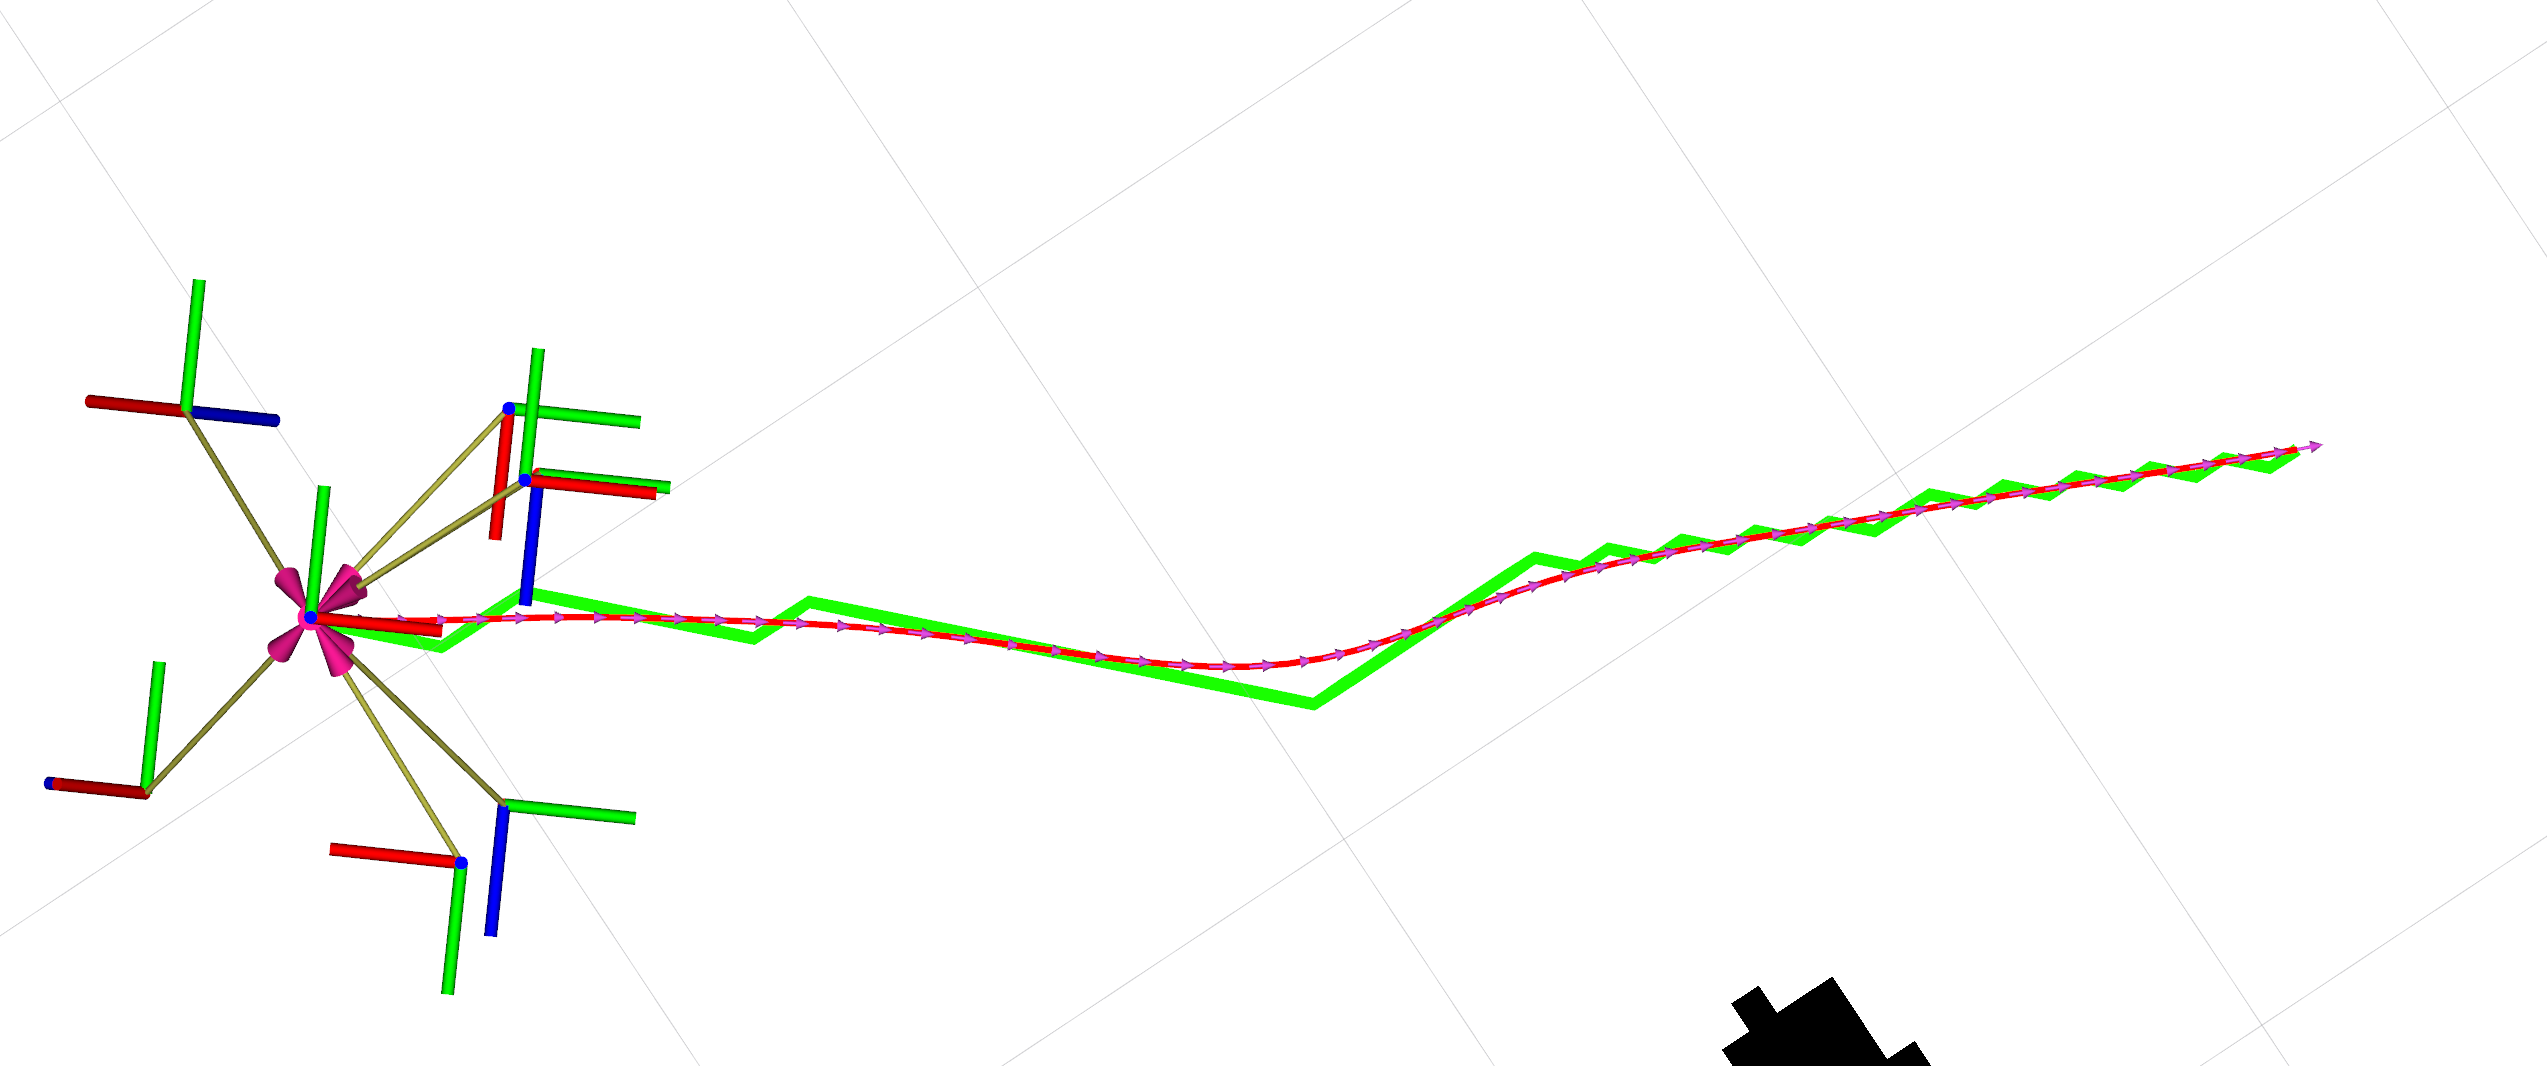
\includegraphics[width=0.85\textwidth]{figures/ch04/path_smoothing_comparison.png}
    \caption{Comparison of the planner output with and without path smoothing. The unsmoothed trajectory contains abrupt heading changes and unnecessary zigzags, while the smoothed trajectory follows a more continuous and natural path, resulting in improved tracking performance and reduced steering effort.}
    \label{fig:path_smoothing_comparison}
\end{figure}
\begin{figure}[H]
\centering
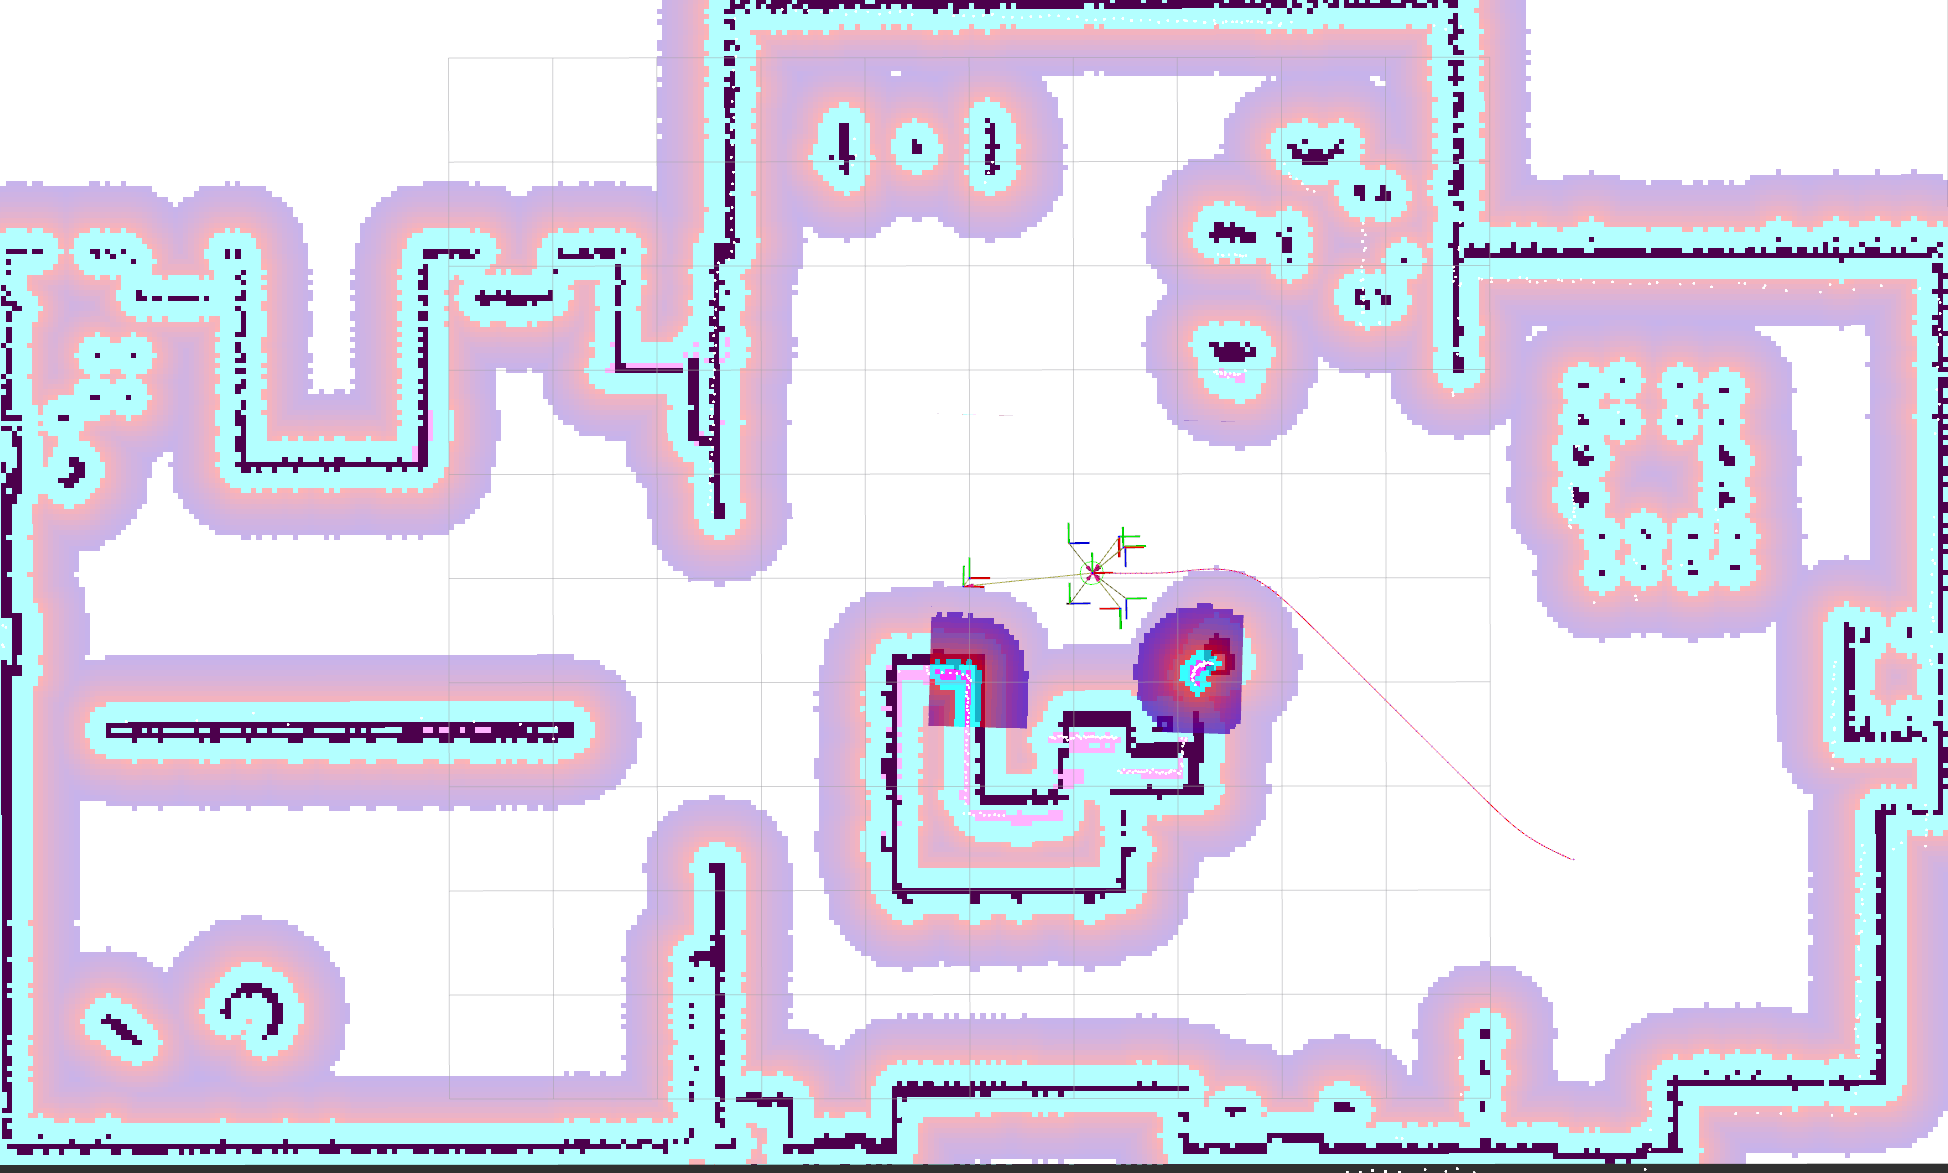
\includegraphics[width=\textwidth]{figures/ch04/global_path.png}
\caption{Smac Planner 2D global path visualised in RViz. The cost-travel multiplier steers the path to the corridor centre, and the inline smoother rounds sharp A* waypoints into a continuous curve.}
\label{fig:global_path}
\end{figure}

\begin{figure}[H]
    \centering
    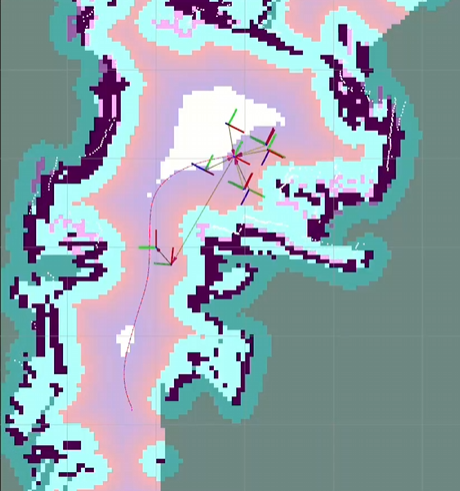
\includegraphics[width=0.6\textwidth]{figures/ch04/real_path_planning.png}
    \caption{Real-world path planning and execution on the physical robot footprint.}
    \label{fig:real_path_creation}
\end{figure}

% ─────────────────────────────────────────────────────────────────────────────
\subsection*{Local Costmap}
\label{sec:local_costmap}
% ─────────────────────────────────────────────────────────────────────────────

While the global costmap provides a complete world model for long-horizon path planning, it is too coarse and too infrequently updated to react to dynamic obstacles that appear mid-trajectory. The \emph{local costmap} solves this problem: it is a small, robot-centred rolling window that follows the robot in real time and feeds the Regulated Pure Pursuit controller with an up-to-date hazard map around the robot's current position.

Key differences from the global costmap are summarised in Table~\ref{tab:costmap_compare}.

\begin{table}[H]
\centering
\caption{Global vs.\ Local Costmap design choices.}
\label{tab:costmap_compare}
\renewcommand{\arraystretch}{1.3}
\begin{tabular}{lll}
\hline
\textbf{Parameter} & \textbf{Global Costmap} & \textbf{Local Costmap} \\
\hline
\texttt{global\_frame}  & \texttt{map}   & \texttt{odom} \\
Window type            & Fixed full map & Rolling $3 \times 3$~m window \\
\texttt{update\_frequency} & 1.0~Hz      & 5.0~Hz \\
\texttt{publish\_frequency} & 1.0~Hz     & 2.0~Hz \\
\texttt{resolution}    & 0.05~m/cell    & 0.05~m/cell \\
\texttt{robot\_radius} & 0.20~m         & 0.10~m \\
\texttt{inflation\_radius} & 0.65~m     & 0.55~m \\
Observation source     & \texttt{/scan} & \texttt{/scan}
\hline
\end{tabular}
\end{table}

\paragraph{Design choices explained.}
\begin{itemize}\itemsep=2pt
    \item \textbf{\texttt{global\_frame: odom}}: The local costmap is anchored to the \texttt{odom} frame rather than \texttt{map}, so its position is not perturbed by AMCL particle-filter jumps. This prevents sudden phantom obstacles being injected into the controller's view when localisation re-converges.
    \item \textbf{Rolling $3 \times 3$~m window}: The window is large enough to preview obstacles several lookahead distances ahead, yet small enough to update at 5~Hz without excessive CPU cost. At the maximum wheelchair speed of $0.3$~m/s the robot travels only $0.06$~m per update cycle, so no obstacle can enter the window unseen.
    \item \textbf{Dual filtered scan sources}: Instead of the merged \texttt{/scan} topic used by the global costmap, the local costmap subscribes directly to \texttt{/scan\_left\_filtered} and \texttt{/scan\_right\_filtered} --- the individually self-filtered beams from each LiDAR. Using the pre-filtered per-sensor topics here gives finer spatial resolution around the robot's immediate periphery and avoids any merge latency.
    \item \textbf{Smaller robot radius ($0.10$~m vs.\ $0.20$~m)}: The local costmap uses a tighter footprint so the controller can navigate narrow domestic corridors without the robot being marked as self-colliding. The global planner retains the conservative $0.20$~m radius to keep long-horizon paths well centred.
    \item \textbf{No static layer}: The local costmap contains only \texttt{obstacle\_layer} and \texttt{inflation\_layer}. Including a static layer would prevent the controller from moving through regions that the SLAM map marks as occupied but that are actually clear (e.g.\ after furniture has been moved), since the local costmap has no mechanism to override static cells.
\end{itemize}

The key local costmap configuration parameters, taken from \texttt{controller\_server.yaml}, are summarized in Table~\ref{tab:local_costmap_yaml}.

\begin{table}[H]
\centering
\caption{Local costmap configuration parameters (\texttt{controller\_server.yaml}).}
\label{tab:local_costmap_yaml}
\renewcommand{\arraystretch}{1.2}
\begin{tabular}{ll}
\toprule
\textbf{Parameter} & \textbf{Value} \\
\midrule
\texttt{global\_frame} & \texttt{odom} \\
\texttt{rolling\_window} & \texttt{true} \\
\texttt{width} $\times$ \texttt{height} & $3.0 \times 3.0$~m \\
\texttt{update\_frequency} & $5.0$~Hz \\
\texttt{publish\_frequency} & $2.0$~Hz \\
\texttt{resolution} & $0.05$~m/cell \\
\texttt{robot\_radius} & $0.10$~m \\
\texttt{plugins} & Obstacle, Inflation \\
\texttt{observation\_sources} & \texttt{scan\_left\_filtered}, \texttt{scan\_right\_filtered} \\
\texttt{obstacle\_max\_range} & $2.5$~m \\
\texttt{raytrace\_max\_range} & $3.0$~m \\
\texttt{inflation\_radius} & $0.55$~m \\
\texttt{cost\_scaling\_factor} & $3.0$ \\
\bottomrule
\end{tabular}
\end{table}

% ─────────────────────────────────────────────────────────────────────────────
\section{Block 6: Costmap Inflation}
\label{sec:costmap}
% ─────────────────────────────────────────────────────────────────────────────

\subsection*{Why Inflation Matters}

A raw obstacle map treats every occupied cell as equally forbidden and every free cell as equally traversable. Without inflation, a path computed on such a binary map will pass within millimetres of walls and furniture corners, since there is no cost gradient to discourage proximity. For a wheelchair carrying a human passenger this is unacceptable: sensor noise alone is often enough to cause a collision at such margins.

\subsection*{Inflation Layer}
A raw obstacle map treats every occupied cell as equally forbidden and every free cell as equally traversable. Without inflation, a path computed on such a binary map could pass within millimetres of walls and furniture corners, since there is no cost gradient discouraging proximity. For a wheelchair carrying a human passenger this is unacceptable: sensor noise alone is often enough to cause a collision at such margins.

The inflation layer addresses this by expanding obstacles outward, assigning gradually decreasing costs around each occupied cell instead of marking only the cell itself as forbidden. This produces a smooth cost gradient rather than a sharp lethal/free boundary, so the global and local planners are discouraged from routing paths close to obstacles even when a geometrically shorter path exists. The width and steepness of this gradient are controlled by the \texttt{inflation\_radius} and \texttt{cost\_scaling\_factor} parameters, set to $0.65$~m and $3.0$ for the global costmap and $0.55$~m and $3.0$ for the local costmap (Tables~\ref{tab:planner_yaml} and~\ref{tab:local_costmap_yaml}).

\begin{figure}[H]
\centering
\begin{subfigure}[t]{0.48\textwidth}
    \centering
    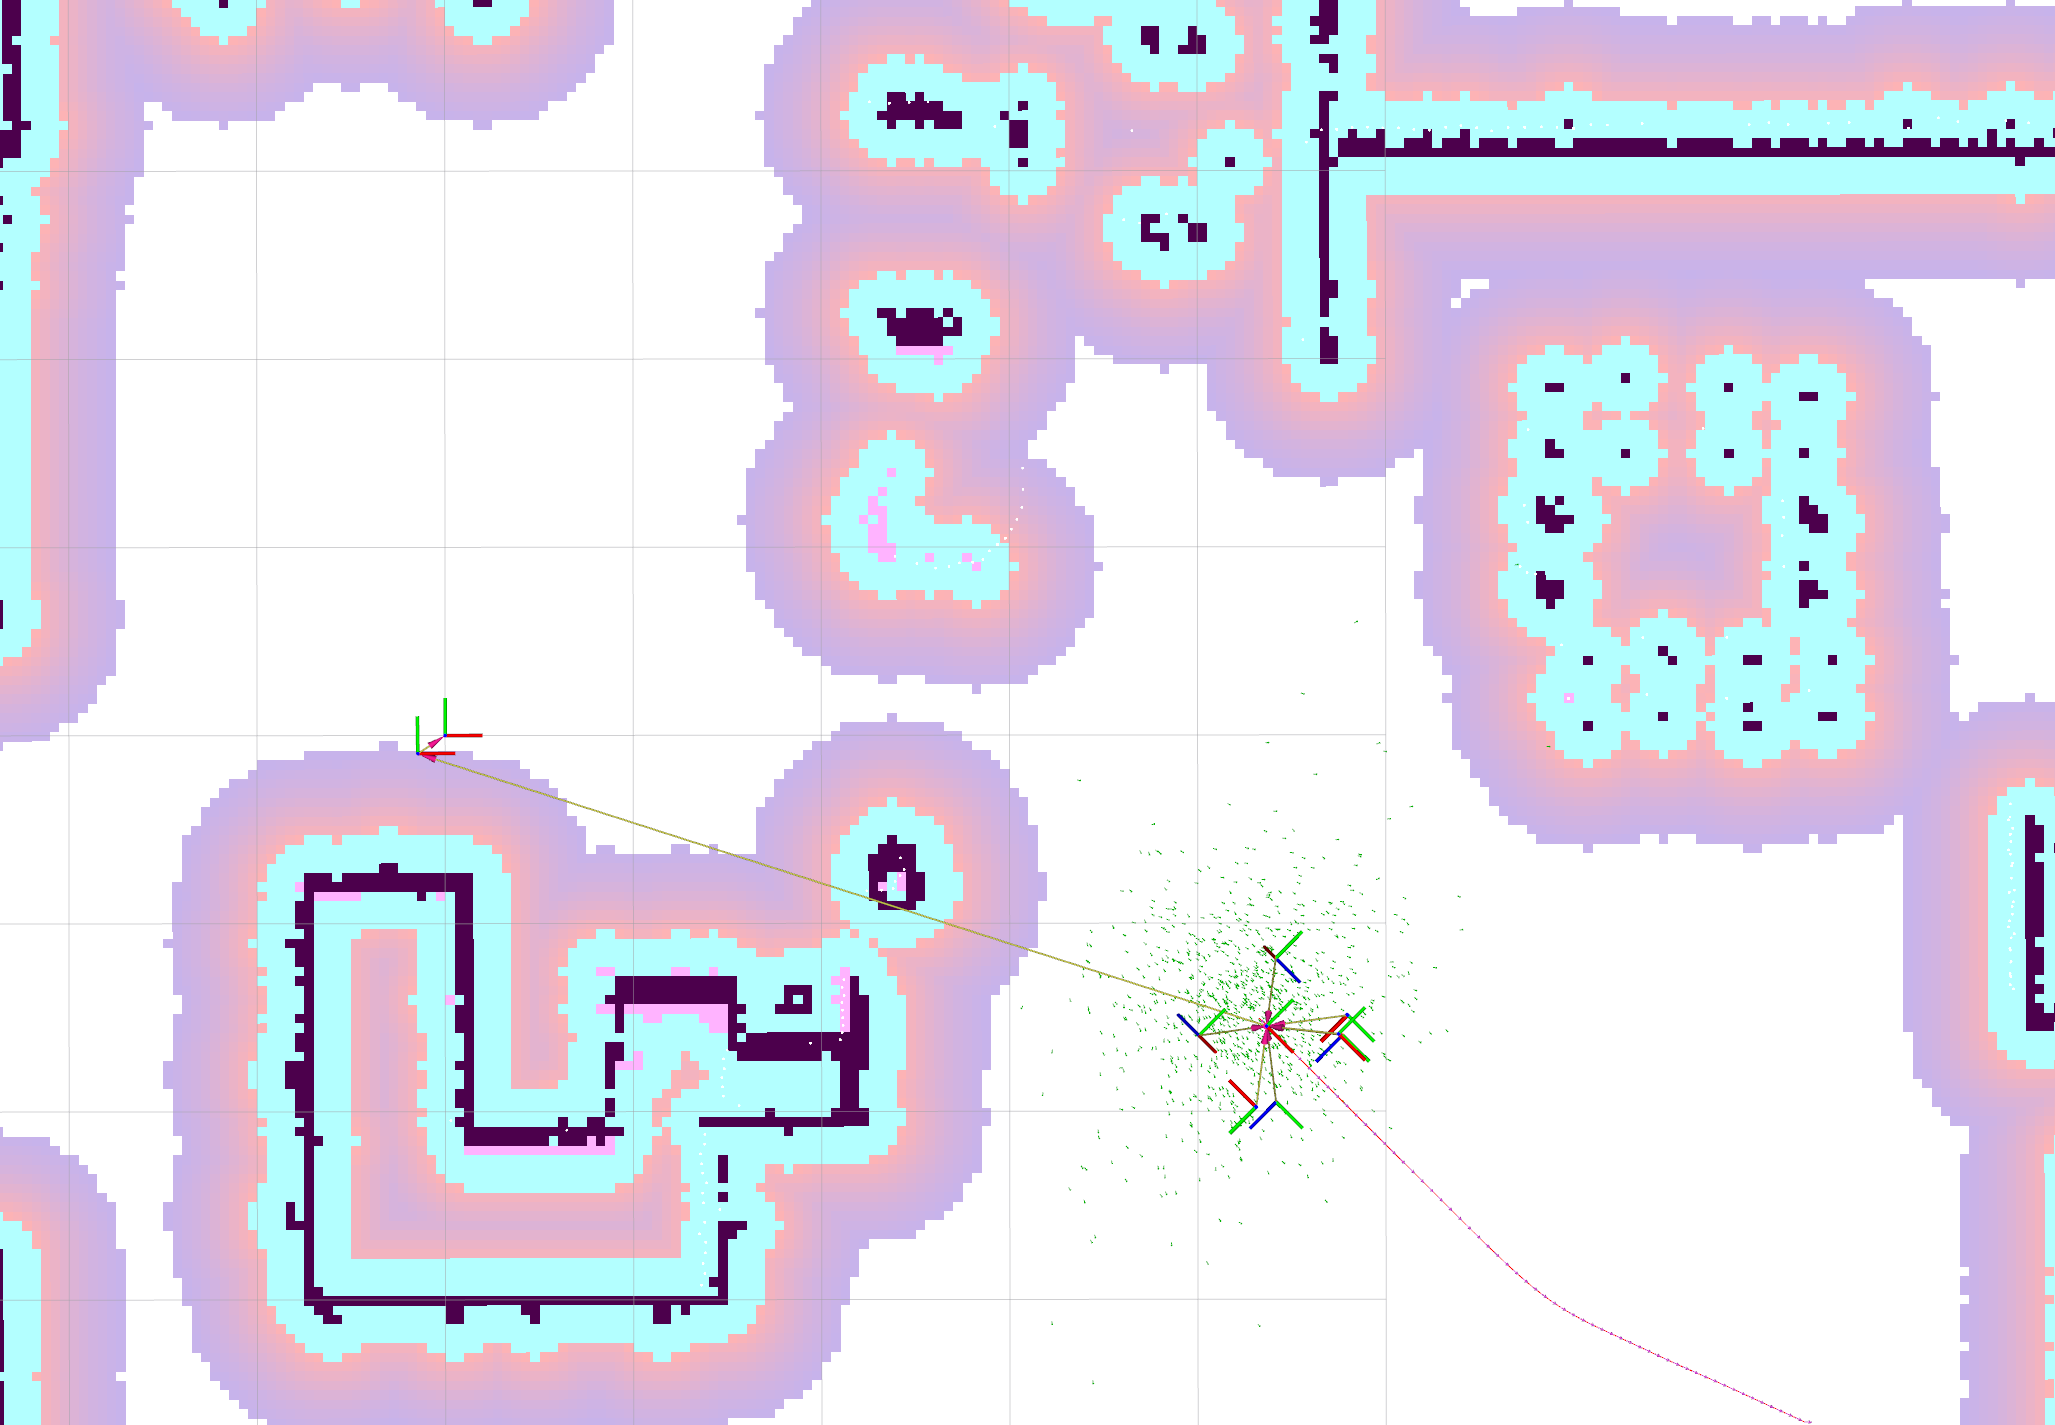
\includegraphics[width=\linewidth]{figures/ch04/with_inflation_far.png}
    \caption{Robot far from the obstacle.}
    \label{fig:inflation_far}
\end{subfigure}
\hfill
\begin{subfigure}[t]{0.48\textwidth}
    \centering
    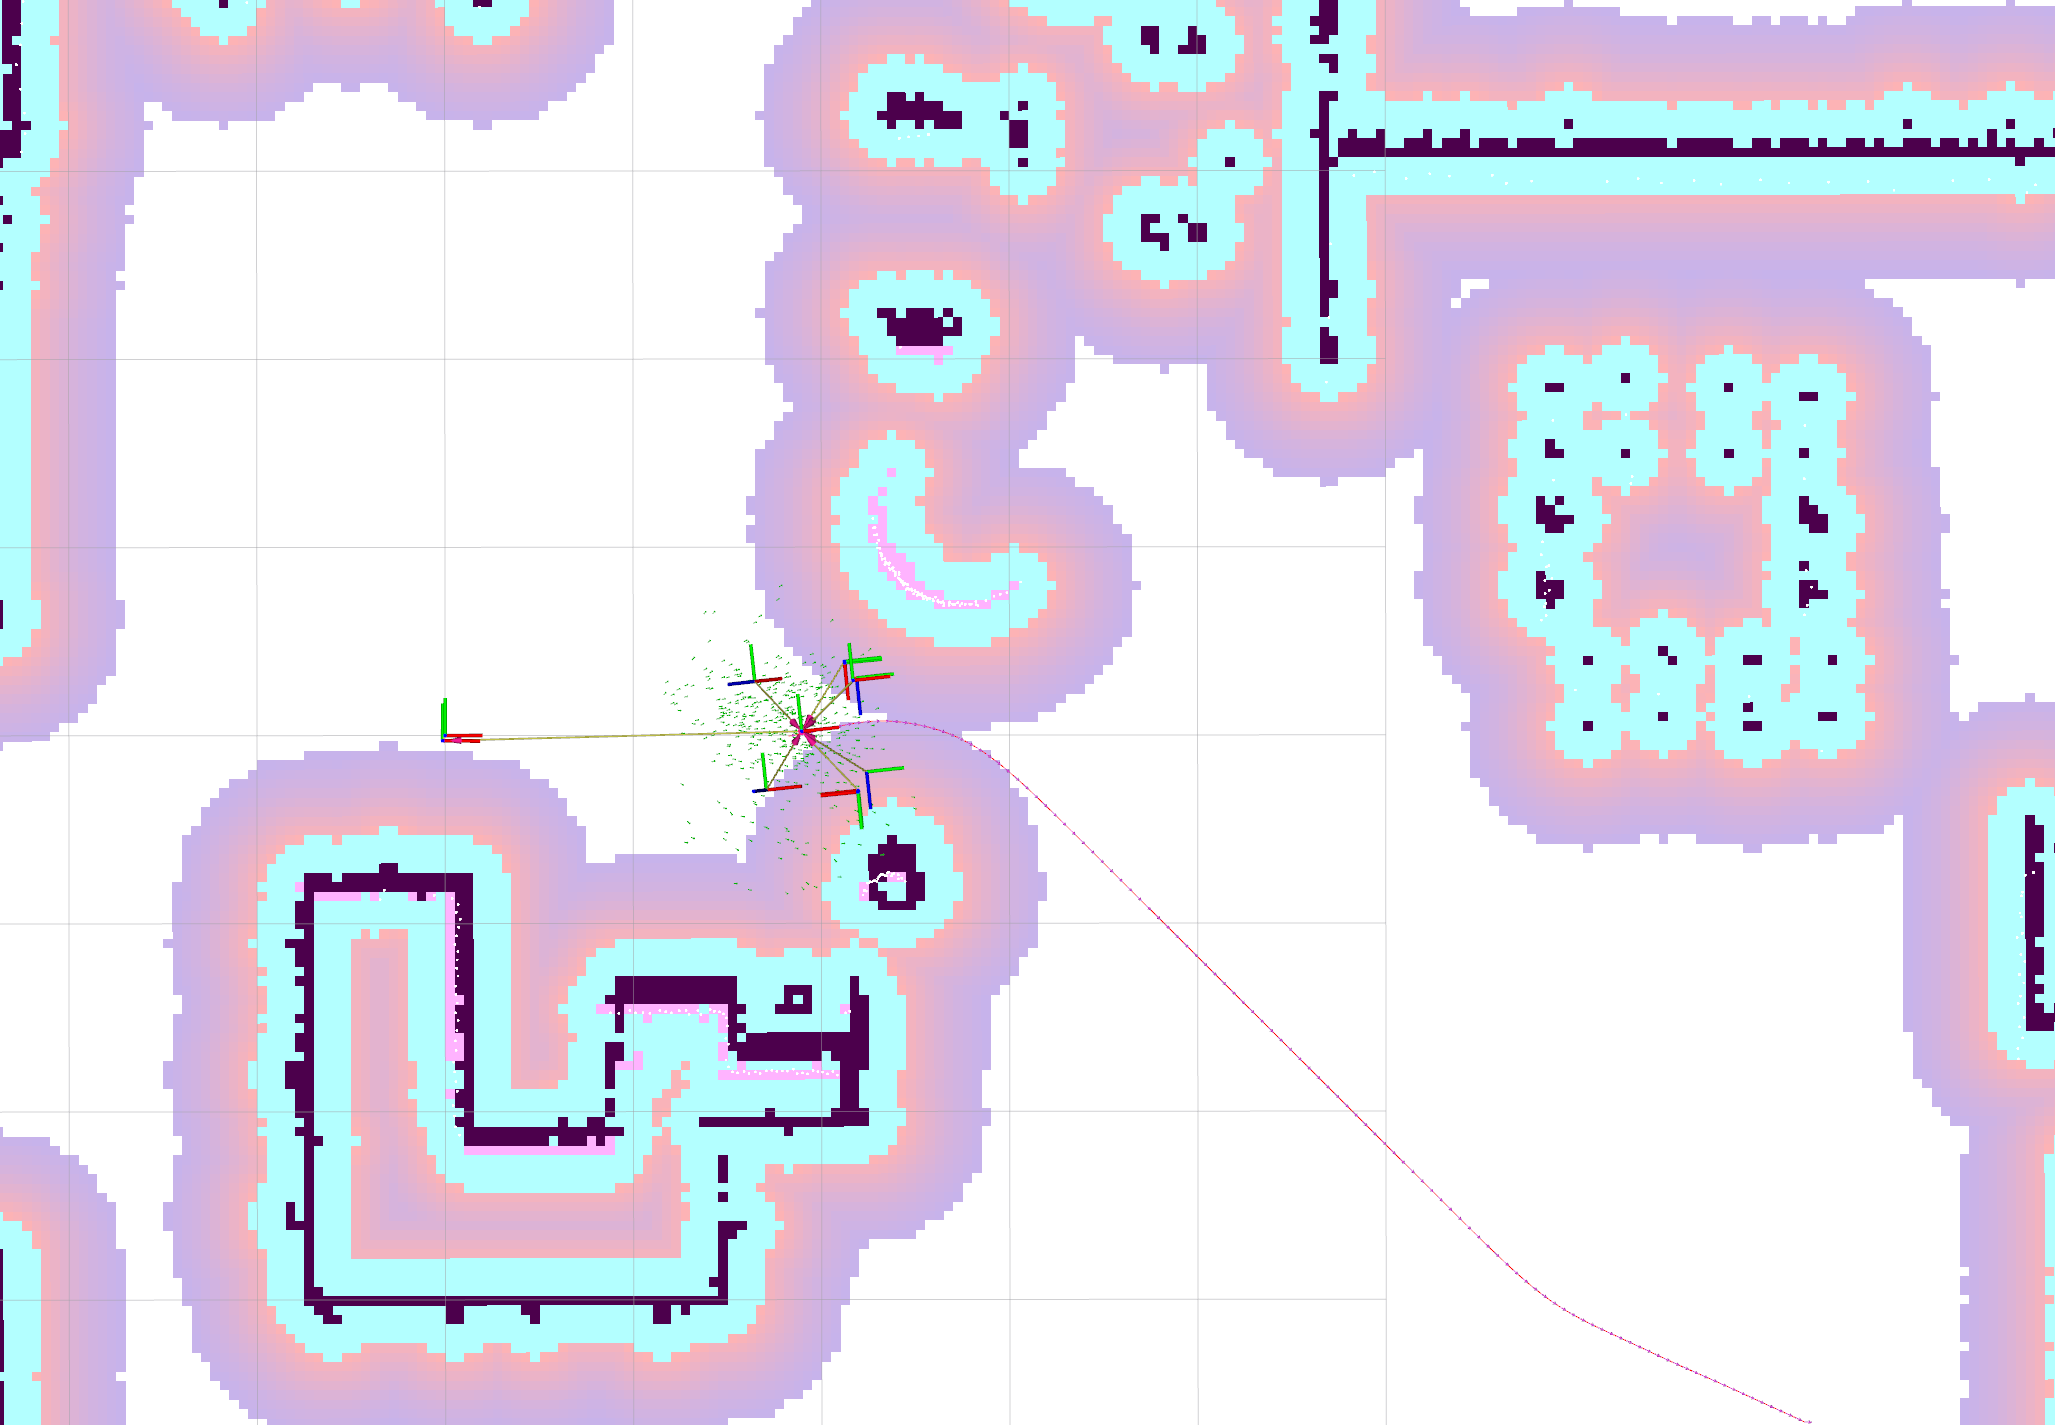
\includegraphics[width=\linewidth]{figures/ch04/with_inflation_close.png}
    \caption{Robot near the obstacle.}
    \label{fig:inflation_close}
\end{subfigure}
\caption{Local costmap with the inflation layer enabled. The coloured halo surrounding each obstacle represents the decaying cost gradient produced by the \texttt{InflationLayer} plugin, which the planner and controller treat as an increasingly penalized region as the robot approaches.}
\label{fig:inflation}
\end{figure}

As shown in Figure~\ref{fig:inflation}, the inflated region forms a soft safety buffer around each obstacle: cells immediately adjacent to an obstacle carry a high cost, while cost decreases smoothly with distance until it reaches zero at the edge of the inflation radius. This gradient is what allows the Regulated Pure Pursuit controller (Section~\ref{sec:planner}) to naturally favor the centre of corridors and maintain clearance from walls and furniture, rather than requiring hard-coded minimum-distance rules.
\section{Block 7: Local Trajectory Control}

The trajectory controller node (\texttt{controller\_server}) uses the Regulated Pure Pursuit Controller (\texttt{nav2\_regulated\_pure\_pursuit\_controller::RegulatedPurePursuitController}) configured in \texttt{controller\_server.yaml}.

Pure Pursuit is a geometric path-tracking algorithm in which the robot continuously selects a target point located a fixed look-ahead distance along the reference path. The controller computes the curvature required to steer the robot toward this target, allowing it to converge smoothly back to the path as it moves forward. Figure~\ref{fig:pp_concept} illustrates this basic concept.

\begin{figure}[H]
    \centering
    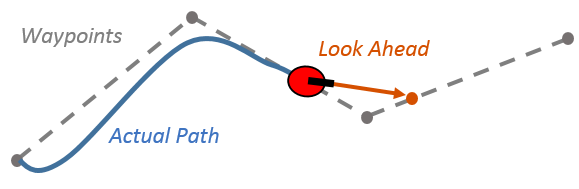
\includegraphics[width=0.75\linewidth]{figures/ch04/pure_pursuit_concept.png}
    \caption{Concept of the Pure Pursuit algorithm. The controller continuously selects a look-ahead point on the reference path and computes the steering command required to drive the robot toward it.}
    \label{fig:pp_concept}
\end{figure}

A naive Pure Pursuit controller drives the robot at a constant linear velocity regardless of the path geometry. While this approach performs adequately on gentle curves, it often overshoots sharp corners or becomes unstable when navigating narrow indoor environments. Adaptive Pure Pursuit improves tracking by varying the look-ahead distance according to the path curvature. Regulated Pure Pursuit extends this idea by additionally regulating the robot's linear velocity based on path curvature and obstacle proximity, enabling safer and more accurate navigation. Figure~\ref{fig:pp_comparison} compares the behavior of the three controllers.

\begin{figure}[H]
    \centering
    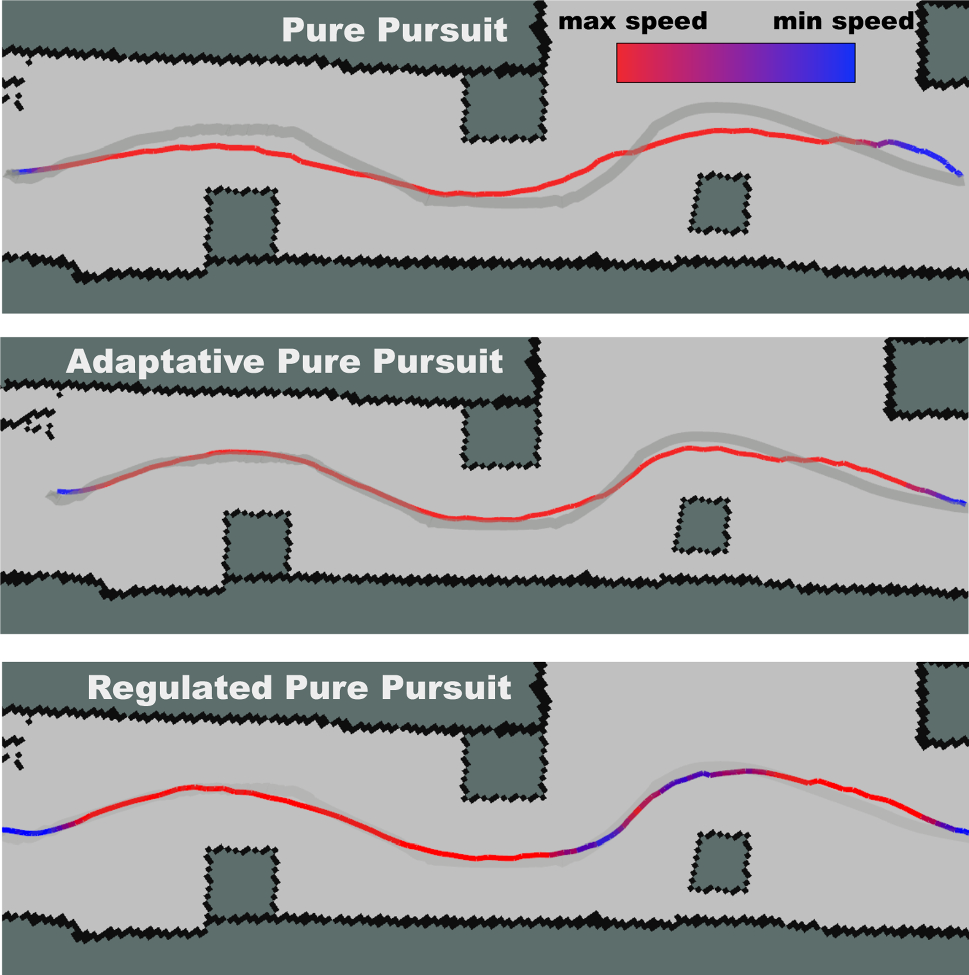
\includegraphics[width=\linewidth,height=0.45\textheight,keepaspectratio]{figures/ch04/pure_pursuit_comparison.png}
    \caption{Comparison of Pure Pursuit variants. Standard Pure Pursuit uses a fixed look-ahead distance, Adaptive Pure Pursuit adjusts the look-ahead distance according to the path geometry, and Regulated Pure Pursuit further reduces the robot velocity in high-curvature regions and near obstacles to improve tracking stability and safety.}
    \label{fig:pp_comparison}
\end{figure}

The controller parameters in \texttt{controller\_server.yaml} limit the indoor speed to $0.3$\,m/s, configure a look-ahead distance of $0.6$\,m, set goal checking tolerances to $0.25$\,m, and enable collision detection.


\section{Human Follower Mode}

\subsection{Subsystem Overview}
\label{sec:overview}

The Person-Following Subsystem lets Sanad autonomously track and follow a companion or caregiver, without requiring the user to drive the wheelchair manually. Because the subsystem relies directly on the Nav2 stack for dynamic path planning, obstacle avoidance, and global localization, this follow mode is specifically designed for \textbf{indoor navigation only}. 

It is implemented as two ROS~2 nodes connected by a single message type, \texttt{TrackedPerson}:
 
\begin{itemize}
    \item \textbf{Perception Node} --- detects and tracks people in RGB-D frames, estimates depth, selects one target, and publishes it on \texttt{/person/target}.
    \item \textbf{Follow Node} --- back-projects the target into a 3D map-frame pose via TF2, and sends \texttt{NavigateToPose} goals to Nav2 to maintain a fixed following distance.
\end{itemize}

 Figure~\ref{fig:pipeline_overview} illustrates this flow end to end, from raw RGB-D frames to the Nav2 goals that ultimately drive the wheelchair.

\begin{figure}[H]
    \centering
    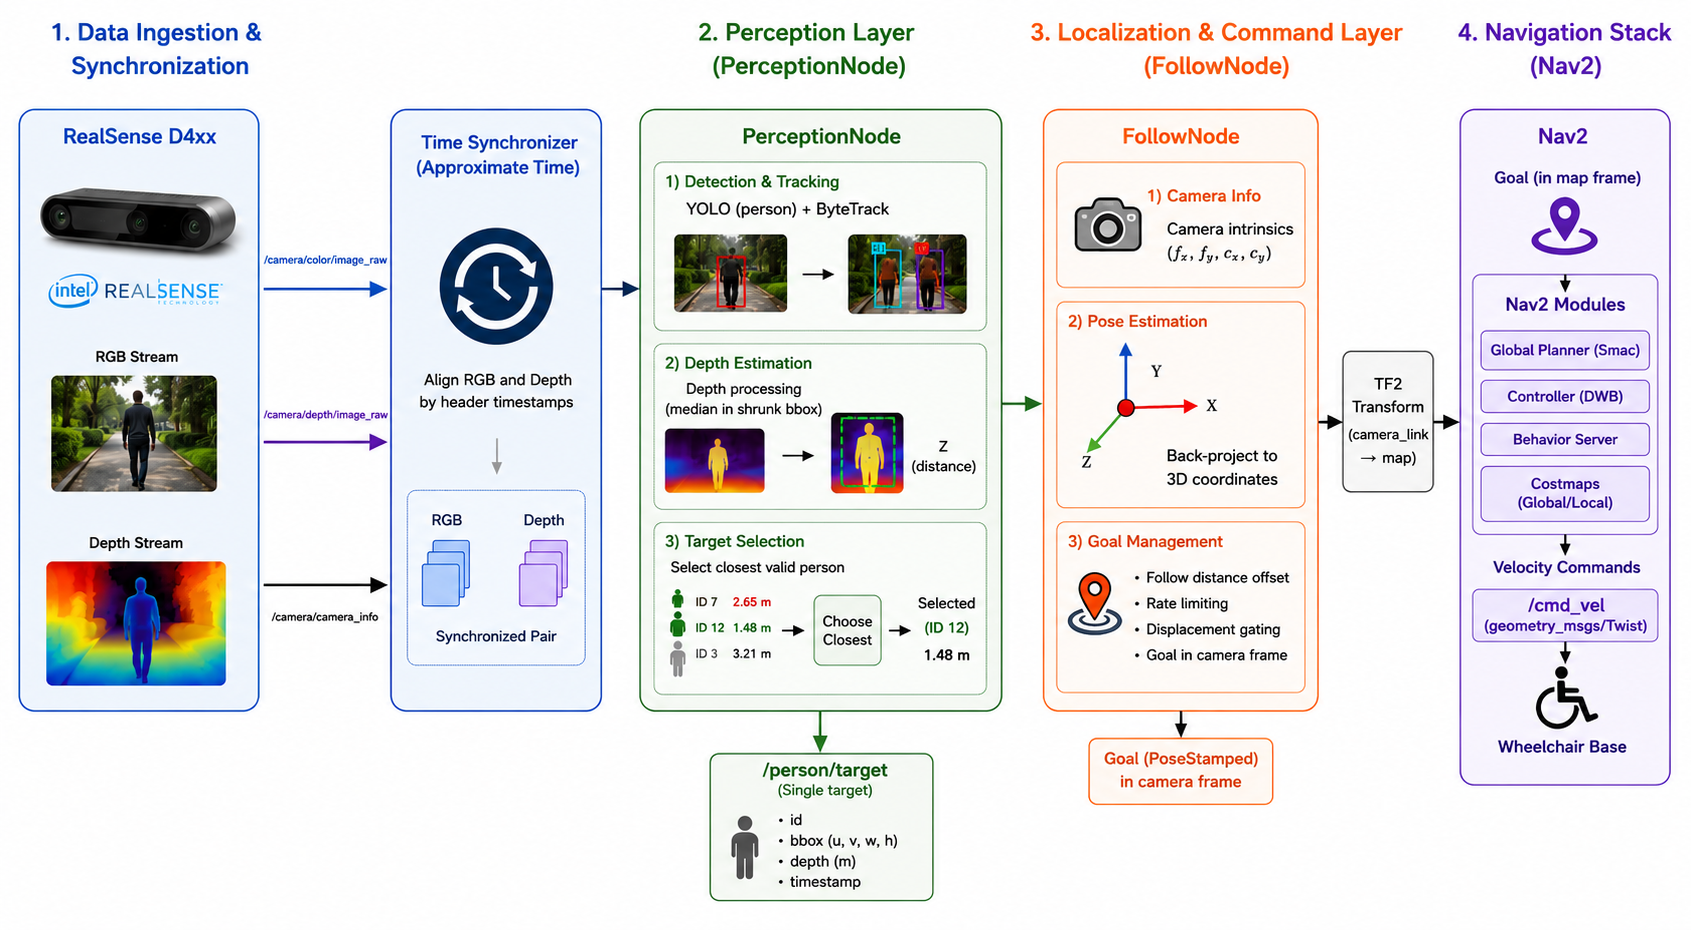
\includegraphics[width=1.1\linewidth]{figures/ch04/human_following.png}
    \caption{Person-following pipeline overview.}
    \label{fig:pipeline_overview}
\end{figure}
 
Splitting perception from goal management keeps each node independently testable (the Follow Node can be exercised with a synthetic \texttt{/person/target} publisher, with no camera or GPU required) and lets either be replaced without touching the other.
 
\subsection{Detection \& Tracking}
\label{sec:detection}
 
Detection uses a YOLO26n model restricted to the person class (\texttt{classes=[0]}, confidence $\geq 0.40$, IoU $\leq 0.45$), run in FP16 on GPU with an automatic CPU fallback if CUDA is unavailable.
 
Tracking uses ByteTrack (\texttt{.track(..., persist=True)}) rather than an appearance-based tracker such as DeepSORT: ByteTrack associates detections by motion and IoU rather than a learned embedding, avoiding a second network per frame --- an appropriate trade-off given the embedded GPU budget and the single-nearby-target use case, at the cost of weaker recovery from long occlusions (Section~\ref{sec:tradeoffs}).
 
Inference runs on a dedicated thread rather than inside the image-sync callback, fed by a single-slot (\texttt{maxlen=1}) queue: if a new frame arrives before the previous one finishes processing, the older frame is dropped. This bounds latency at the cost of not processing every captured frame --- the right trade-off for a real-time control loop. A periodic sync-rate counter and a watchdog (no frames for $>5$~s) surface camera or synchronization problems early.

\begin{figure}[H]
    \centering
    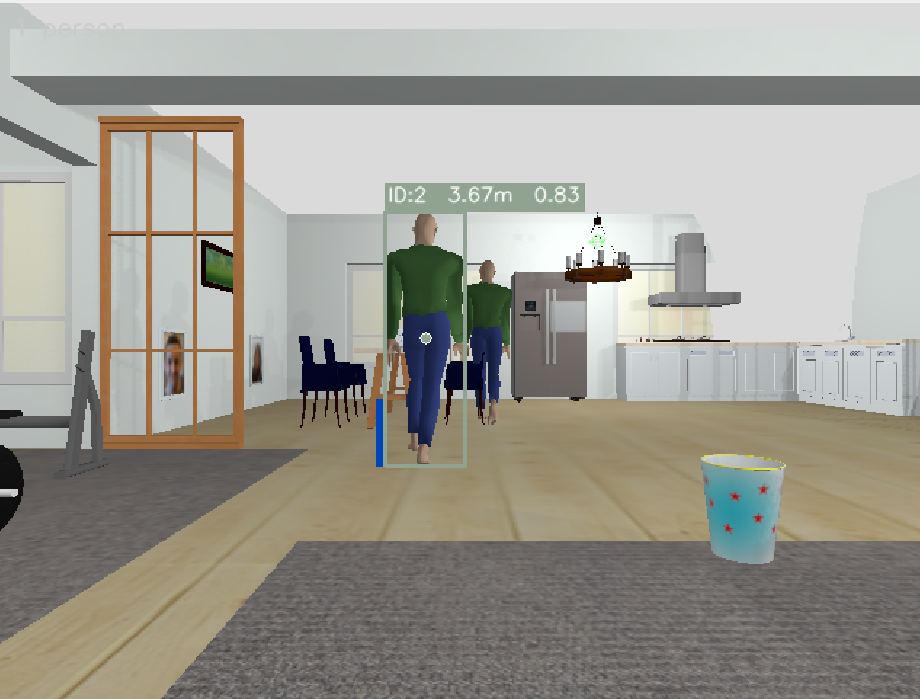
\includegraphics[width=0.8\linewidth]{figures/ch04/human_tracked.png}
    \caption{Real-time person detection and tracking visualization in simulation. The bounding box displays the assigned Track ID (ID: 2), the estimated median depth (3.67m), and the YOLO detection confidence score (0.83).}
    \label{fig:detection_result}
\end{figure}

\subsubsection{TensorRT Optimization}
\label{sec:tensorrt_optimization}

The transition from a standard PyTorch framework model to an optimized TensorRT engine yielded substantial improvements across all primary performance metrics, ensuring the perception pipeline does not throttle the downstream control loop. The quantitative performance improvements are detailed in Table~\ref{tab:tensorrt_metrics}.

\begin{table}[htbp]
\centering
\caption{TensorRT optimization performance comparison}
\label{tab:tensorrt_metrics}
\begin{tabular}{llll}
\toprule
\textbf{Metric} & \textbf{Baseline (\texttt{.pt})} & \textbf{Optimized (\texttt{.engine})} & \textbf{Performance} \\
\midrule
First Inference (Cold Start) & $961.7$~ms & $84.9$~ms & $11\times$ faster \\
Steady-State Inference      & $25$--$45$~ms & $12$--$22$~ms & $\sim 2\times$ faster \\
GPU Memory Footprint         & $72$~MB   & $4$~MB    & $18\times$ reduction \\
\bottomrule
\end{tabular}
\end{table}

These optimizations ensure that perception no longer becomes the bottleneck of the navigation pipeline, while leaving sufficient GPU resources for localization and Nav2.
 
\subsection{Depth-Aware 3D Localization}
\label{sec:localization}
 
Per-pixel depth at a bounding-box centroid is unreliable near edges, where structured-light sensors produce bleed artifacts. Depth is therefore sampled from the inner 60\% of each box (falling back to a small centroid kernel for degenerate boxes), filtered to the sensor's reliable range, and reduced to the median of the surviving pixels; fewer than 5 valid pixels marks the estimate invalid rather than returning a guess.
 
The validated depth and centroid pixel are back-projected to 3D using the pinhole model:
 
\begin{align}
X &= \frac{(u - c_x)\,Z}{f_x} \\
Y &= \frac{(v - c_y)\,Z}{f_y} \\
Z &= \text{depth}
\end{align}
 
with intrinsics captured once from the first \texttt{CameraInfo} message. The point is then transformed from the camera's optical frame to the map frame via TF2, stamped with the image's own timestamp for accuracy. If that exact-time transform isn't yet available --- typically only just after startup --- the node falls back to the latest available transform rather than dropping the frame, trading a small lateral error during fast rotation for not losing the follow lock in the first seconds of operation. The pose is flattened to $z=0$ for Nav2; orientation is computed later, during goal construction (Section~\ref{sec:goal_management}).
 
\subsection{Target Selection \& Persistence}
\label{sec:target_selection}
 
With multiple people potentially in frame, and no input mechanism for the user to point at one, the Follow Node picks a single target and holds it via a small latch:
 

 
% =============================================================
% Target Selection State Machine — TikZ diagram
% Required packages (add to your document preamble if not already present):
%   \usepackage{tikz}
%   \usetikzlibrary{positioning, arrows.meta}
% Paste this figure block in place of the commented-out
% \includegraphics line in Section 4 (Target Selection & Persistence).
% =============================================================
 % The full acquisition, hold, and release logic is summarized as a state machine in Figure~\ref{fig:target_state_machine}.
 
\begin{figure}[h!]
\centering
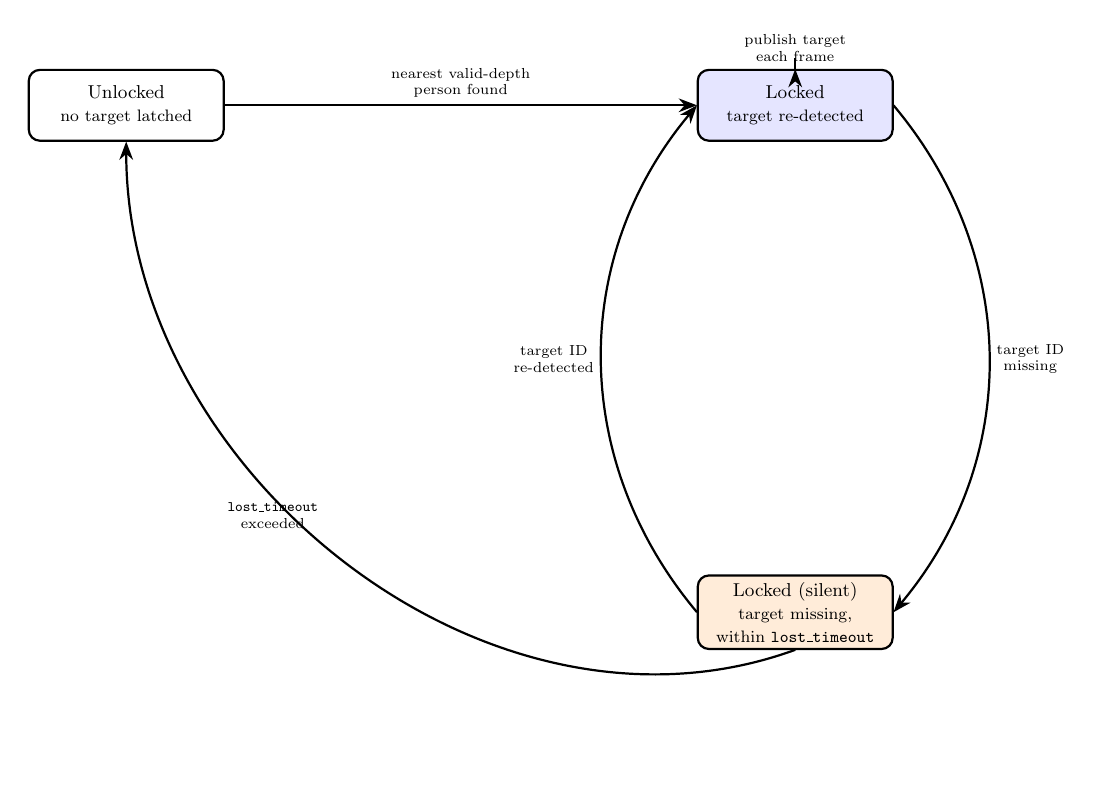
\begin{tikzpicture}[
    >=Stealth,
    scale=0.75, every node/.style={scale=0.75},
    node distance=5.5cm and 6cm,
    state/.style={
        rectangle, rounded corners, draw=black, thick,
        minimum width=3.3cm, minimum height=1.2cm,
        align=center, font=\small
    },
    locked/.style={state, fill=blue!10},
    lost/.style={state, fill=orange!15},
    lbl/.style={font=\scriptsize, align=center}
]
 
% --- States ---
\node[state]                         (unlocked) {Unlocked\\\footnotesize no target latched};
\node[locked, right=of unlocked]     (locked)   {Locked\\\footnotesize target re-detected};
\node[lost,   below=of locked]       (lost)     {Locked (silent)\\\footnotesize target missing,\\\footnotesize within \texttt{lost\_timeout}};
 
% --- Transitions ---
\draw[->, thick] (unlocked) -- node[lbl, above] {nearest valid-depth\\person found} (locked);
 
\draw[->, thick] (locked.east) to[bend left=40] node[lbl, right, pos=0.5] {target ID\\missing} (lost.east);
 
\draw[->, thick] (lost.west) to[bend left=40] node[lbl, left, pos=0.5] {target ID\\re-detected} (locked.west);
 
\draw[->, thick] (lost.south) to[out=200, in=270] node[lbl, below, pos=0.6] {\texttt{lost\_timeout}\\exceeded} (unlocked.south);
 
% self-loop on Locked: re-detected each frame
\draw[->, thick] (locked.north) to[out=70, in=110, looseness=6] node[lbl, above] {publish target\\each frame} (locked.north);
 
\end{tikzpicture}
\caption{Target selection state machine.}
\label{fig:target_state_machine}
\end{figure}

\begin{itemize}
    \item \textbf{Unlocked} --- among tracks with valid depth, the nearest person is selected and their \texttt{track\_id} latched.
    \item \textbf{Locked} --- each frame, the tracker list is searched for that ID; if found, it is published and the lock refreshed. Nearer people are ignored while locked.
    \item \textbf{Lost} --- if the ID is missing, the lock is held (publishing nothing) for up to \texttt{lost\_timeout} before releasing back to Unlocked.
\end{itemize}
 
Latching --- rather than re-selecting ``nearest'' every frame --- prevents flicker if a bystander briefly passes closer than the actual companion, and the grace period absorbs brief ByteTrack ID drops from occlusion. The trade-off, discussed further in Section~\ref{sec:tradeoffs}: no person re-identification, so the system tracks \emph{whoever was nearest at acquisition}, not a verified identity.
 
\subsection{Goal Management --- the ``Step-Chasing'' Pattern}
\label{sec:goal_management}
 
Because the followed person is always moving, the Follow Node never commits to one fixed destination; it continuously re-evaluates their position and, when warranted, issues a short incremental goal trailing them by a fixed standoff distance --- a sequence of ``next step'' goals rather than one long path.
 
To avoid replanning on every incoming message, three gates must all pass before an update is sent: a rate limit (\texttt{goal\_update\_hz}), a minimum person-displacement (\texttt{min\_person\_disp\_m}, filtering estimation jitter), and a minimum goal-displacement versus the last \emph{sent} goal (\texttt{min\_goal\_disp\_m}, preventing oscillation near the previous gate's threshold). This is the key difference from a naive periodic cancel-and-resend scheme, which would replan on a timer regardless of actual movement.
 
When an update is warranted, any active or \emph{pending} goal (sent but not yet accepted --- a race \texttt{send\_goal\_async()} can otherwise expose) is cancelled before the replacement is sent. The new goal sits along the robot$\rightarrow$person line, short by the standoff distance, facing the person:
 
\begin{align}
\text{scale} &= \frac{\text{dist} - d_{\text{follow}}}{\text{dist}} \\
\text{goal} &= \text{robot} + (dx, dy)\cdot \text{scale} \\
\psi &= \operatorname{atan2}(dy, dx)
\end{align}
 
If the robot is already closer than $d_{\text{follow}}$, no goal is sent.
 
\subsection{Robustness Features}
\label{sec:robustness}
 
\begin{itemize}
    \item \textbf{Accept/cancel race guard} --- a pending-goal flag prevents acting on a goal handle before Nav2 confirms acceptance.
    \item \textbf{Dual-layer timeout} --- the Perception Node's lock timeout covers ``this person briefly left frame''; an independent Follow Node watchdog, reset on every target message, covers ``the perception pipeline stopped publishing entirely.''
    \item \textbf{Manual terminal-status check} --- ROS~2 Humble's \texttt{ClientGoalHandle} has no \texttt{.done()} method, so completion is checked against explicit terminal \texttt{GoalStatus} values instead.
    \item \textbf{Depth validity gating} --- tracks without a valid depth reading are skipped rather than back-projected.
    \item \textbf{Throttled logging} --- repeated warnings/errors are rate-limited so a persistent fault doesn't flood the log.
    \item \textbf{Optional debug pose topic} --- for RViz monitoring; no effect on control if disabled.
\end{itemize}
 
\subsection{Design Trade-offs Discussion}
\label{sec:tradeoffs}
 
Across the subsystem, the same stance recurs: stability and motion smoothness were prioritized over reacting to every available signal instantly.
 
\begin{table}[h!]
\centering
\caption{Design trade-offs across the Person-Following subsystem.}
\label{tab:tradeoffs}
\begin{tabular}{|p{0.20\textwidth}|p{0.18\textwidth}|p{0.26\textwidth}|p{0.22\textwidth}|}
\hline
\textbf{Decision} & \textbf{Alternative} & \textbf{Why} & \textbf{Accepted limitation} \\
\hline
ByteTrack & Appearance-based (DeepSORT) & Lower compute, fits single-target use case & Weaker recovery after long occlusion \\
\hline
Frame-dropping inference thread & Synchronous inference in callback & Bounded latency & Not every frame is processed \\
\hline
Latched target persistence & Re-select nearest each frame & No flicker between people & No person re-identification \\
\hline
Gated step-chasing goals & Periodic cancel-and-resend & Smoother motion, less planner churn & Small, bounded lag before motion is reflected \\
\hline
TF fallback to latest transform & Strict frame-drop & Following survives startup/reset & Small lateral error during fast rotation \\
\hline
Dual-layer timeout & Single shared timeout & Distinguishes failure causes & Slightly more state to tune \\
\hline
\end{tabular}
\end{table}
 
The two open limitations --- no re-identification, and a small motion lag --- are the accepted cost of that stability, and are natural directions for future work rather than design defects.
 
\subsection{Parameter Reference}
\label{sec:appendix_parameters}
 
\begin{table}[H]
\centering
\caption{Person-following subsystem parameters.}
\label{tab:parameters}
\begin{tabular}{|p{0.32\textwidth}|p{0.13\textwidth}|p{0.45\textwidth}|}
\hline
\textbf{Parameter} & \textbf{Value} & \textbf{Purpose} \\
\hline
\texttt{confidence\_threshold} & 0.40 & Minimum detection confidence \\
\hline
\texttt{iou\_threshold} & 0.45 & NMS overlap threshold \\
\hline
\texttt{depth\_bbox\_shrink} & 0.60 & Bbox fraction sampled for depth \\
\hline
\texttt{depth\_kernel\_size} & 7~px & Fallback centroid window \\
\hline
\texttt{lost\_timeout} (Perception) & 2.0~s & Grace period before releasing target lock \\
\hline
\texttt{follow\_distance\_m} & 1.0~m & Standoff distance behind person \\
\hline
\texttt{min\_person\_disp\_m} & 0.20~m & Min.\ person movement to trigger goal update \\
\hline
\texttt{min\_goal\_disp\_m} & 0.40~m & Min.\ goal displacement before replacing active goal \\
\hline
\texttt{goal\_update\_hz} & 1.0 & Ceiling on goal-update rate \\
\hline
\texttt{lost\_timeout} (Follow watchdog) & 2.0~s & Cancels goal if no target message received \\
\hline
\end{tabular}
\end{table}

\subsection{Visualization}
\label{sec:Visualization}

\begin{figure}[H]
    \centering
    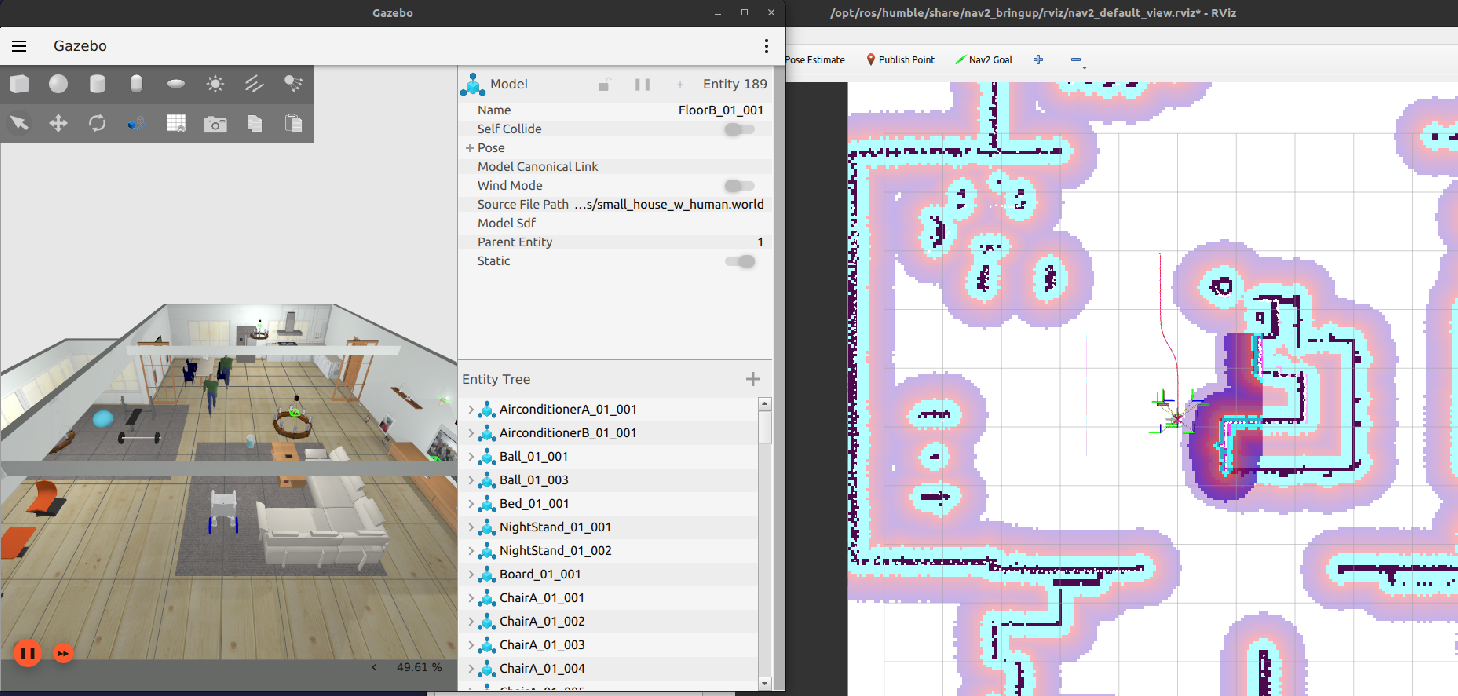
\includegraphics[width=0.9\linewidth]{figures/ch04/human.png}
    \caption{Person-following visalization in simulation}
    \label{fig:human}
\end{figure}




\section{Vision-Language Model}
\label{sec:vlm}
\begin{figure}[H]
\centering
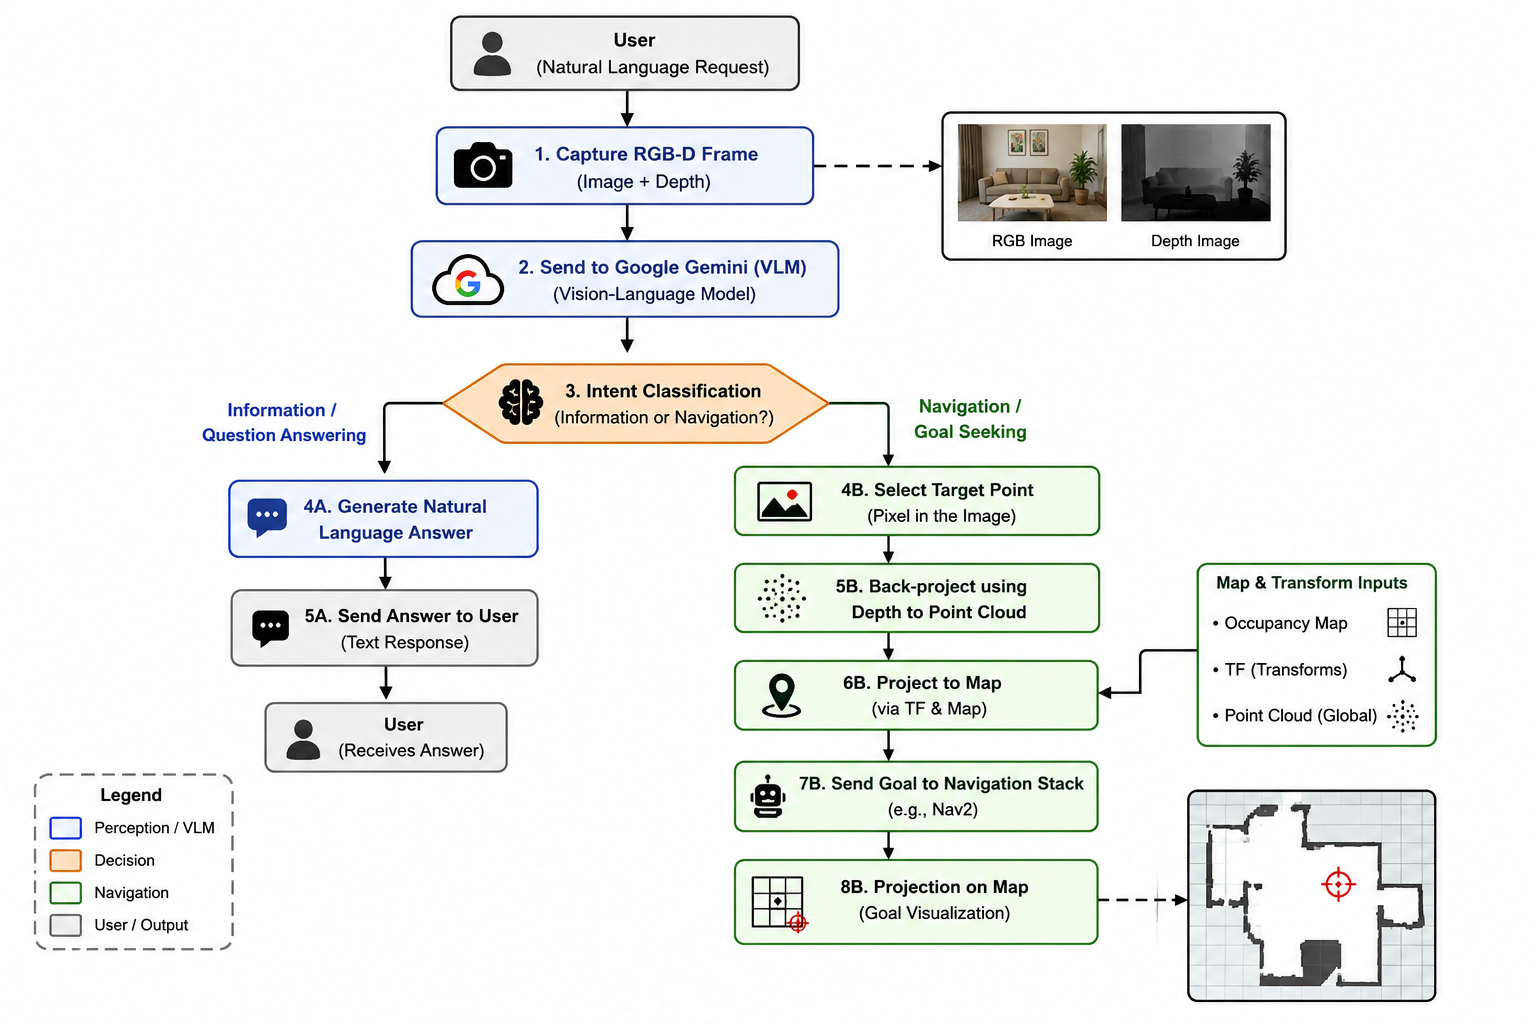
\includegraphics[width=0.85\textwidth]{figures/ch04/vlm_diagram.png}
\caption{Overview of the VLM request pipeline. A captured frame and user request are sent to Gemini, which branches into either a scene-understanding answer or an object-localization result that is back-projected into a Nav2 goal pose.}
\label{fig:vlm_pipeline_diagram}
\end{figure}
To support natural, open-ended interaction beyond fixed voice commands, a Vision-Language Model (VLM) is integrated into the navigation stack. The VLM consumes the live RGB-D stream and a natural-language user query, and supports two distinct modes of operation: \textbf{scene understanding} and \textbf{semantic object navigation}.

\subsection*{Scene Understanding}

In this mode, the user asks an open-ended question about their surroundings (e.g., ``what's on the table in front of me?'' or ``describe the room''). The current camera frame is sent along with the query to Google's Gemini model, which returns a natural-language answer describing the scene. This allows the patient to query their environment conversationally without requiring a predefined vocabulary of objects or locations, and is particularly useful for users with limited mobility or visual impairment who cannot easily inspect their surroundings directly.

\begin{figure}[H]
\centering
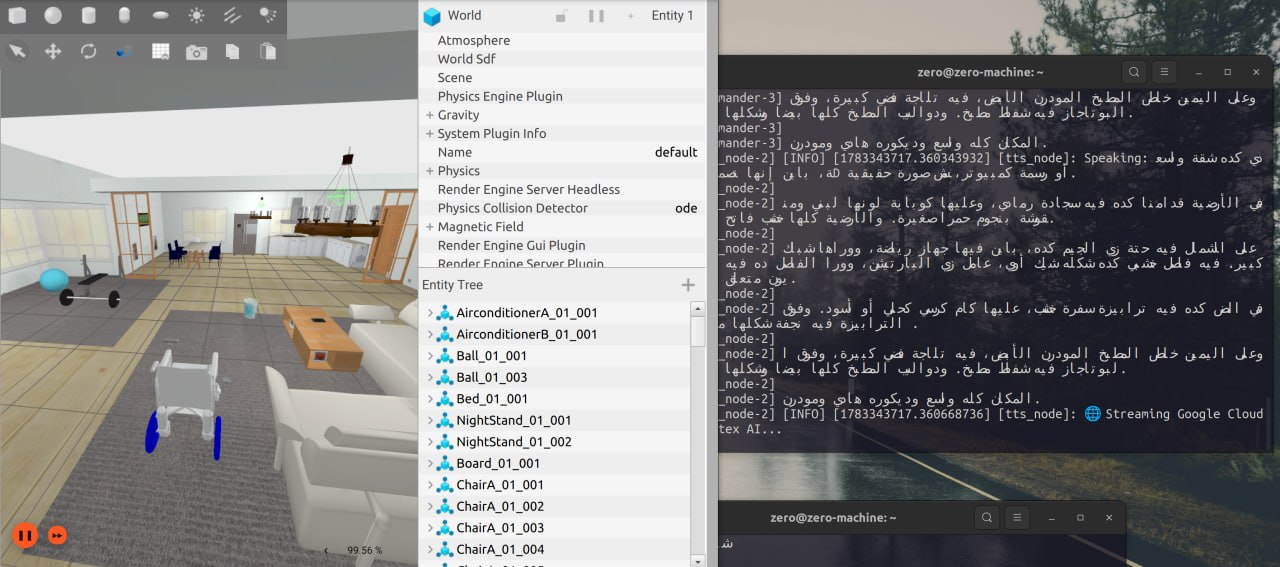
\includegraphics[width=0.85\textwidth]{figures/ch04/vlm_scene_description.jpg}
\caption{Scene understanding mode: the VLM receives the current camera frame together with a user query and returns a natural-language description of the scene via Gemini.}
\label{fig:vlm_scene_description}
\end{figure}

\subsection*{Semantic Object Navigation}

In this mode, the user issues a navigation request referring to an object by description rather than by a fixed map waypoint (e.g., ``take me to the green ball''). The VLM localizes the target object within the current camera frame, identifying its bounding box among possibly multiple candidate objects of similar type. The bounding box centroid is back-projected into a 3D goal pose using the depth stream, following the same pinhole back-projection approach used in the person-following subsystem (Section~\ref{sec:localization}), and the resulting pose is sent to the Nav2 action server as a \texttt{NavigateToPose} goal.

Figure~\ref{fig:vlm_object_selection} illustrates this disambiguation capability: given a scene containing two visually similar objects (a blue ball and a green ball) and the instruction to navigate to the green one, the VLM correctly identifies and targets only the specified object rather than the nearest or first-detected candidate.

\begin{figure}[H]
\centering
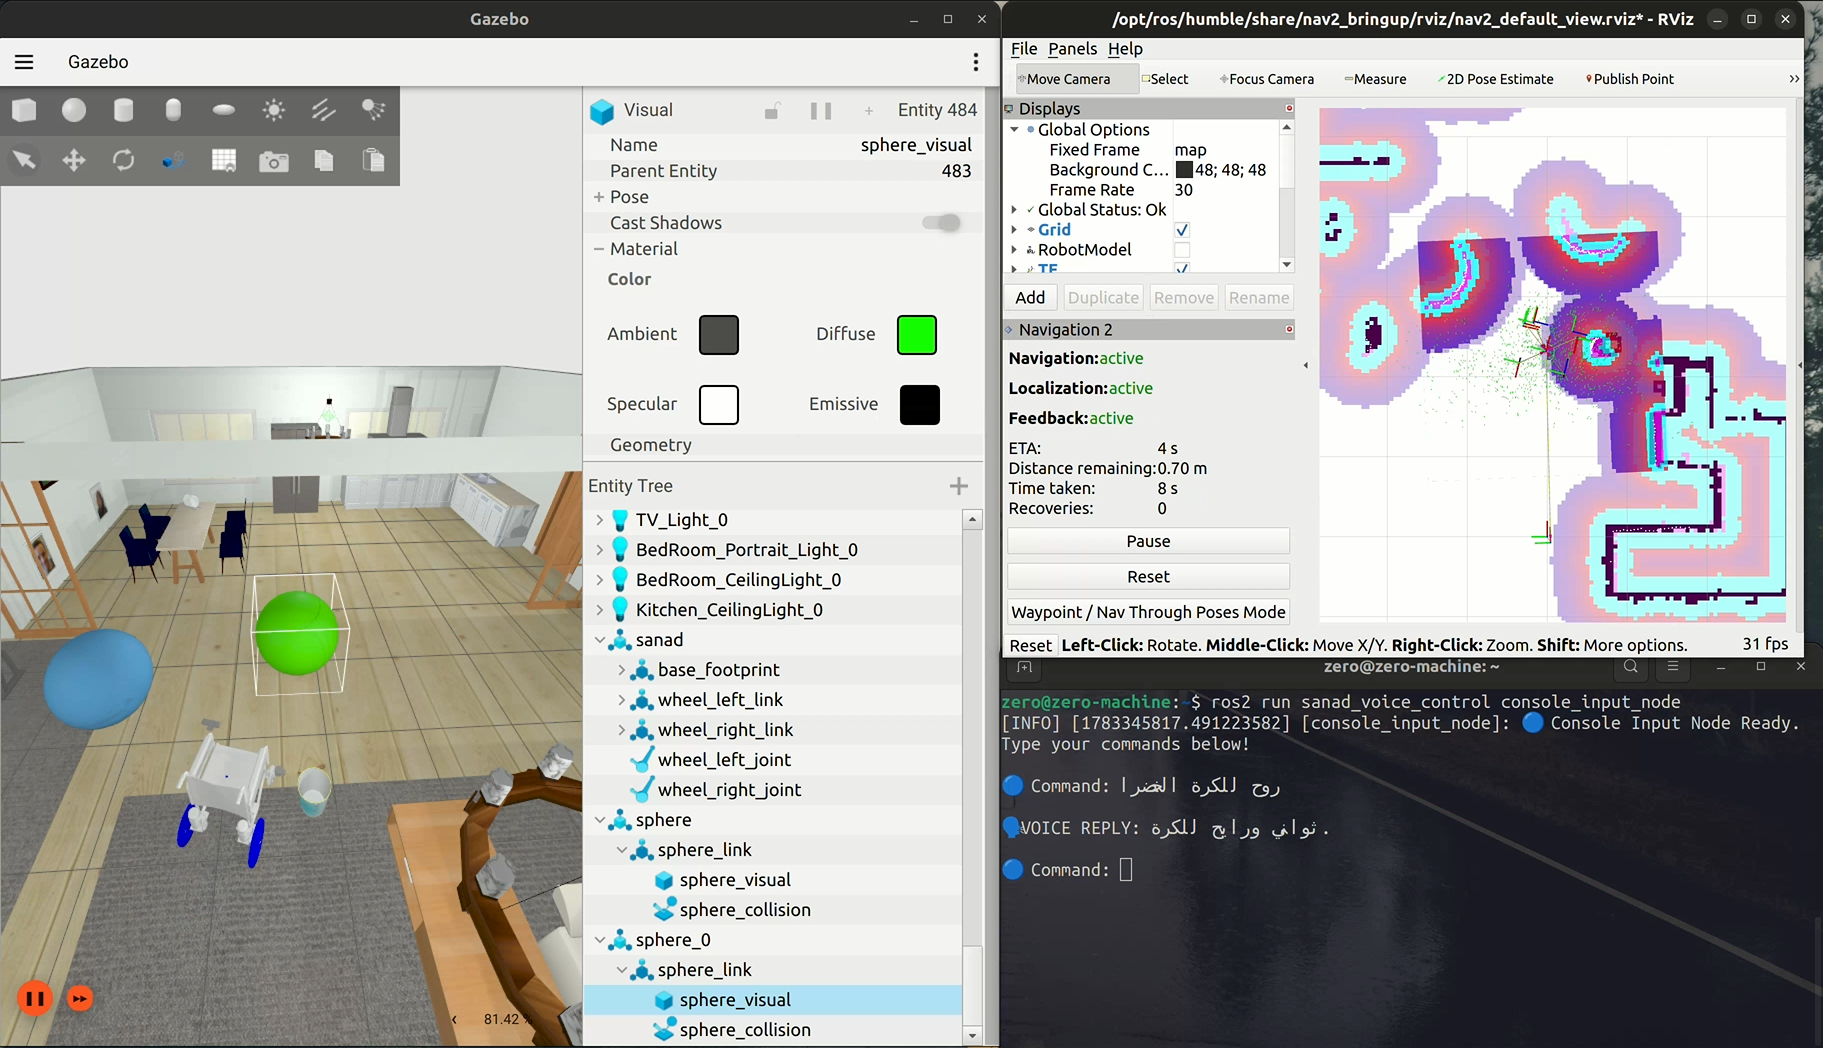
\includegraphics[width=0.85\textwidth]{figures/ch04/vlm_green_ball.png}
\caption{Semantic object navigation mode: given the instruction to navigate to the green ball, the VLM distinguishes between the two candidate objects (blue and green balls) in the scene and selects the correct target for goal generation.}
\label{fig:vlm_object_selection}
\end{figure}

Together, these two modes allow the VLM to serve both as a conversational scene-query interface and as a semantic front end to the navigation stack, extending the fixed voice-command vocabulary described in Chapter 5 with open-vocabulary object reference.
\section{Summary and Transition}
This chapter has detailed the autonomous navigation stack, explaining how the sensor, state estimation, localization, and planning stages coordinate motion. The next chapter, Chapter 5 (Voice Control \& Large Language Model (LLM) Integration), describes how the user communicates natural-language goals to this navigation core.



\chapterseparator{Chapter 5}
\setcounter{chapter}{5}
\chapter*{Chapter (5): Voice Control \& Large Language Model (LLM) Integration}
\addcontentsline{toc}{chapter}{Chapter (5): Voice Control \& Large Language Model (LLM) Integration}
\setcounter{section}{0}

\section{Chapter Preview}
This chapter describes the natural-language voice interface for the Sanad wheelchair. It details the hybrid cloud-edge speech pipeline, including wake-word detection, Speech-to-Text (STT) transcription, Gemini-driven intent parsing, structured command routing, and Text-to-Speech (TTS) response synthesis.

\begin{figure}[htbp]
    \centering
    \resizebox{0.95\textwidth}{!}{
    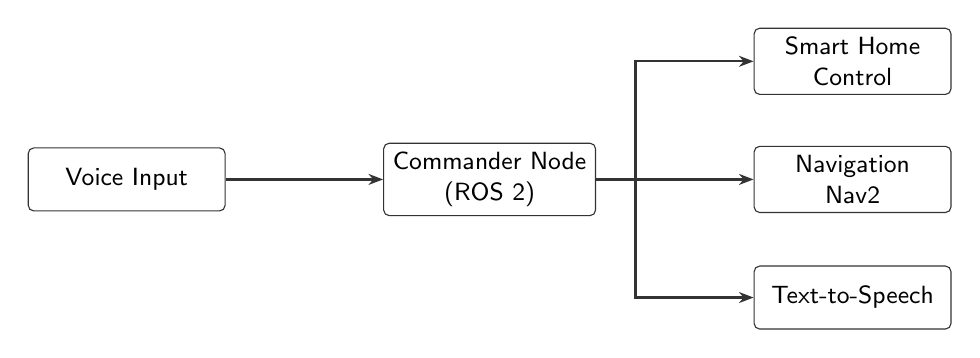
\begin{tikzpicture}[
        node distance=1.5cm and 2cm,
        box/.style={rectangle, draw=black!80, fill=white, minimum height=0.8cm, minimum width=2.5cm, align=center, font=\sffamily\small, rounded corners=2pt},
        arrow/.style={-{Stealth[scale=0.8]}, draw=black!80, thick}
        ]
        
        \node[box] (input) {Voice Input};
        \node[box, right=of input] (cmd) {Commander Node\\(ROS 2)};
        \node[box, right=of cmd, yshift=1.5cm] (sm) {Smart Home\\Control};
        \node[box, right=of cmd] (nav) {Navigation\\Nav2};
        \node[box, right=of cmd, yshift=-1.5cm] (tts) {Text-to-Speech};
        
        \draw[arrow] (input) -- (cmd);
        \draw[arrow] (cmd.east) -- ++(0.5,0) |- (sm.west);
        \draw[arrow] (cmd.east) -- (nav.west);
        \draw[arrow] (cmd.east) -- ++(0.5,0) |- (tts.west);
    \end{tikzpicture}
    }
    \caption{End-to-End Voice Command Pipeline Architecture in ROS 2}
    \label{fig:s1_pipeline}
\end{figure}

The journey of a single voice command follows a highly orchestrated pipeline across several dedicated ROS 2 nodes:
\begin{itemize}
    \item \textbf{Wakeup \& Acquisition:} The system constantly monitors the environment for the specific wake word ("Sanad") using an optimized openWakeWord model. Once triggered, it records the user's spoken audio.
    \item \textbf{Transcription (STT):} The raw audio is either transcribed locally into text using a dedicated Whisper node or sent directly to a multimodal cloud API.
    \item \textbf{Orchestration:} The central \texttt{commander.py} node gathers the transcribed text (or audio path), packages it with the current real-world state of the robot and smart home, and forwards it to the LLM service.
    \item \textbf{Cognitive Processing:} The LLM evaluates the context, determines the user's intent (whether it is an action to perform or a conversational query to answer), and outputs a structured JSON response.
    \item \textbf{Execution \& Routing:} The Commander parses the JSON. If physical actions are required—such as turning on a light, navigating to the kitchen, or sending a Telegram message—it dispatches the appropriate payloads to topics like \texttt{/robot/smarthome\_command} or \texttt{/robot/nav\_command}.
    \item \textbf{Vocal Response (TTS):} Finally, any conversational text generated by the AI is routed to the \texttt{/robot/speak} topic, where it is synthesized into speech and played back to the user.
\end{itemize}

This modular approach ensures that the "brain" of the robot is decoupled from its physical actuators, allowing for scalable and easily updatable code.

\section{The Hybrid Architecture: Cloud-First with Edge Fallback}
One of the most critical requirements for an assistive robot is reliability. If the internet connection drops, the robot must not become entirely incapacitated. To solve this, the Sanad voice pipeline implements a hybrid processing architecture governed by a global \texttt{use\_cloud} launch parameter.

\begin{figure}[htbp]
    \centering
    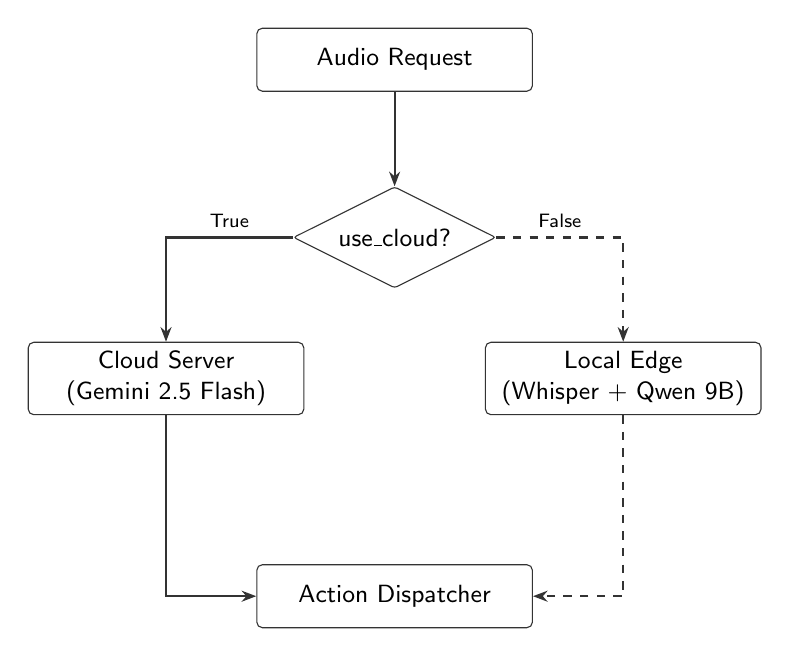
\begin{tikzpicture}[
        node distance=1.2cm and 2cm,
        box/.style={rectangle, draw=black!80, fill=white, minimum height=0.8cm, minimum width=3.5cm, align=center, font=\sffamily\small, rounded corners=2pt},
        decision/.style={diamond, aspect=2, draw=black!80, align=center, font=\sffamily\small, rounded corners=1pt},
        arrow/.style={-{Stealth[scale=0.8]}, draw=black!80, thick},
        dashedarrow/.style={-{Stealth[scale=0.8]}, draw=black!80, thick, dashed}
        ]
        
        \node[box] (req) {Audio Request};
        \node[decision, below=of req] (cloud) {use\_cloud?};
        \node[box, below left=1cm and 0.5cm of cloud] (gemini) {Cloud Server\\(Gemini 2.5 Flash)};
        \node[box, below right=1cm and 0.5cm of cloud] (local) {Local Edge\\(Whisper + Qwen 9B)};
        \node[box, below=3.5cm of cloud] (dispatch) {Action Dispatcher};

        \draw[arrow] (req) -- (cloud);
        \draw[arrow] (cloud.west) -| node[above, near start, font=\sffamily\scriptsize] {True} (gemini.north);
        \draw[dashedarrow] (cloud.east) -| node[above, near start, font=\sffamily\scriptsize] {False} (local.north);
        \draw[arrow] (gemini.south) |- (dispatch.west);
        \draw[dashedarrow] (local.south) |- (dispatch.east);
    \end{tikzpicture}
    \caption{Cloud-First with Edge Fallback Routing Logic}
    \label{fig:s2_hybrid}
\end{figure}

Depending on the state of this parameter, the system dynamically routes its cognitive and audio tasks between high-performance cloud servers and local edge computing.

\subsection{The Cloud Path (High Performance)}
When \texttt{use\_cloud} is active, the system leverages Google GenAI's Vertex AI.
\begin{itemize}
    \item \textbf{Multimodal LLM:} The system bypasses local transcription entirely. The recorded audio file path (e.g., \texttt{audio://...}) is intercepted by the \texttt{llm\_node.py}, which reads the audio bytes and sends them directly to the \texttt{gemini-2.5-flash} model. The model processes the audio and text context simultaneously, resulting in faster and highly accurate intent parsing.
    \item \textbf{Streaming TTS:} For voice output, the system connects to the \texttt{gemini-2.5-flash-preview-tts} model. Instead of waiting for the entire audio file to generate, the TTS node opens a continuous \texttt{sounddevice} output stream, playing audio chunks in real-time the millisecond they arrive over the network.
\end{itemize}

\subsection{The Edge Fallback (Offline Mode)}
If cloud services are disabled or unavailable, the system gracefully falls back to a powerful, fully localized stack.
\begin{itemize}
    \item \textbf{Local STT:} The audio is routed to a dedicated ROS 2 node running \texttt{whisper.cpp} with a quantized model (\texttt{ggml-large-v3-q5\_0.bin}). It transcribes the audio into text locally before passing it to the Commander.
    \item \textbf{Local LLM (Qwen 3.5 9B):} The text prompt is sent to a local REST API endpoint hosted by Koboldcpp. For the core local reasoning engine, the system utilizes the Qwen 3.5 9B model. Qwen 3.5 9B is an extremely efficient multimodal foundation model that provides an excellent balance of speed and reasoning capabilities, outperforming many larger models on complex tasks while comfortably running on edge hardware. This local LLM processes the prompt and returns the same standardized JSON structure expected by the system.
    \item \textbf{Local TTS:} The robot's response is routed to a local installation of Piper TTS, which synthesizes a \texttt{.wav} file offline and plays it through the system's speakers.
\end{itemize}

\section{Multilingual Support \& Dynamic Language Adaptation}
Sanad is designed to be fundamentally language-agnostic, breaking down communication barriers by dynamically mirroring the user's spoken language. This is achieved through a globally tracked language state that influences every stage of the pipeline.

\begin{figure}[htbp]
    \centering
    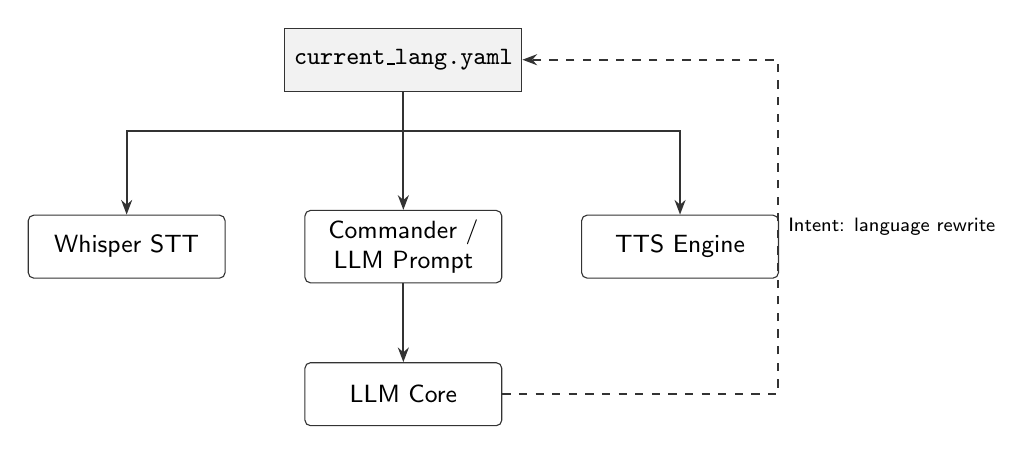
\begin{tikzpicture}[
        node distance=1.5cm,
        box/.style={rectangle, draw=black!80, fill=white, minimum height=0.8cm, minimum width=2.5cm, align=center, font=\sffamily\small, rounded corners=2pt},
        file/.style={rectangle, draw=black!80, fill=gray!10, minimum height=0.8cm, minimum width=3cm, align=center, font=\ttfamily\small, rounded corners=0pt},
        arrow/.style={-{Stealth[scale=0.8]}, draw=black!80, thick},
        dashedarrow/.style={-{Stealth[scale=0.8]}, draw=black!80, thick, dashed}
        ]
        
        \node[file] (state) {current\_lang.yaml};
        \node[box, below=1.5cm of state] (cmd) {Commander /\\LLM Prompt};
        \node[box, left=1cm of cmd] (stt) {Whisper STT};
        \node[box, right=1cm of cmd] (tts) {TTS Engine};
        \node[box, below=1cm of cmd] (llm) {LLM Core};
        
        \draw[arrow] (state.south) -- ++(0,-0.5) -| (stt.north);
        \draw[arrow] (state.south) -- (cmd.north);
        \draw[arrow] (state.south) -- ++(0,-0.5) -| (tts.north);
        \draw[arrow] (cmd) -- (llm);
        \draw[dashedarrow] (llm.east) -- ++(3.5,0) |- node[pos=0.25, right, font=\sffamily\scriptsize] {Intent: language rewrite} (state.east);
    \end{tikzpicture}
    \caption{Multilingual State Tracking and Dynamic Adaptation}
    \label{fig:s3_multilingual}
\end{figure}

\subsection{State Tracking}
The current active language is tracked via a persistent state variable (\texttt{current\_lang}) mapped to a configuration file (\texttt{current\_lang.yaml}). Out of the box, the system maps codes to full languages, supporting Arabic (ar), English (en), French (fr), German (de), Spanish (es), and Italian (it).

\subsection{Dynamic Pipeline Adaptation}
When a user speaks, the language state dictates how the system behaves across three distinct layers:
\begin{itemize}
    \item \textbf{STT Layer:} When the local Whisper node transcribes audio, it reads the \texttt{current\_lang.yaml} file and passes the appropriate \texttt{-l} (language) flag to the \texttt{whisper.cpp} binary. This heavily optimizes transcription speed and accuracy by restricting the model's focus to the expected language.
    \item \textbf{LLM Prompting Layer:} The Commander node dynamically injects the active language into the AI's system prompt. Placeholders like \texttt{\{LANGUAGE\_NAME\}} and \texttt{\{LANGUAGE\_CODE\}} are replaced with values such as "Arabic" and "ar". Because Qwen 3.5 9B has native multilingual capabilities across 201 languages, it easily adapts to this context, forcing both the JSON outputs and the conversational chat to be exclusively in the target language.
    \item \textbf{Real-Time Switching:} The language is not hardcoded. The LLM is given the authority to update the system language via an intent command. If the user says, "Let's speak in English," the LLM outputs a JSON control intent setting the \texttt{target} to \texttt{language} and the \texttt{action} to \texttt{en}. The Commander parses this, overwrites the \texttt{current\_lang.yaml} file, and instantly shifts the entire robot's operational language for the very next interaction.
\end{itemize}

Because the core models (both Gemini in the cloud and Qwen locally) are inherently multilingual, general conversational queries (such as asking for a recipe or how an engine works) bypass hardware action routers and are simply answered organically in whatever language the user has established.

\section{Wake Word Detection \& Audio Acquisition}
The entry point for all human-robot interaction in the Sanad system is the \texttt{wakeup\_node.py}, which is responsible for continuously monitoring the environment without consuming excessive computing resources.

\begin{figure}[htbp]
    \centering
    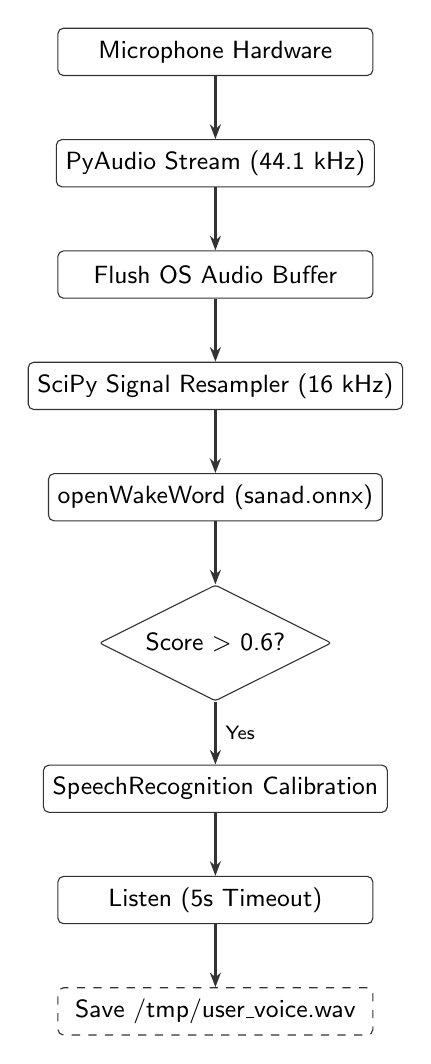
\begin{tikzpicture}[
        node distance=0.8cm,
        box/.style={rectangle, draw=black!80, fill=white, minimum height=0.6cm, minimum width=4cm, align=center, font=\sffamily\small, rounded corners=2pt},
        decision/.style={diamond, aspect=2, draw=black!80, align=center, font=\sffamily\small, rounded corners=1pt},
        arrow/.style={-{Stealth[scale=0.8]}, draw=black!80, thick}
        ]
        
        \node[box] (mic) {Microphone Hardware};
        \node[box, below=of mic] (py) {PyAudio Stream (44.1 kHz)};
        \node[box, below=of py] (flush) {Flush OS Audio Buffer};
        \node[box, below=of flush] (resamp) {SciPy Signal Resampler (16 kHz)};
        \node[box, below=of resamp] (oww) {openWakeWord (sanad.onnx)};
        \node[decision, below=of oww] (trigger) {Score $>$ 0.6?};
        \node[box, below=of trigger] (sr) {SpeechRecognition Calibration};
        \node[box, below=of sr] (listen) {Listen (5s Timeout)};
        \node[box, below=of listen, dashed] (wav) {Save /tmp/user\_voice.wav};

        \draw[arrow] (mic) -- (py);
        \draw[arrow] (py) -- (flush);
        \draw[arrow] (flush) -- (resamp);
        \draw[arrow] (resamp) -- (oww);
        \draw[arrow] (oww) -- (trigger);
        \draw[arrow] (trigger.south) -- node[right, font=\sffamily\scriptsize] {Yes} (sr.north);
        \draw[arrow] (sr) -- (listen);
        \draw[arrow] (listen) -- (wav);
    \end{tikzpicture}
    \caption{Digital Signal Processing (DSP) Flow for Wake Word Detection}
    \label{fig:s4_wakeword}
\end{figure}

To achieve this, the node runs a dedicated listening loop in a background thread, ensuring that the primary ROS 2 event loop is never blocked. The acquisition process follows several precise steps to guarantee accurate triggering and clear audio recording:

\begin{itemize}
    \item \textbf{Wake Word Detection:} The system uses openWakeWord, an open-source, low-resource audio recognition framework. It loads a custom ONNX model (\texttt{sanad.onnx}) trained specifically to recognize the robot's name. To ensure the robot responds accurately without false activations, the model was trained on custom audio datasets. As shown in Figure \ref{fig:wakeword_training}, the model quickly converges, achieving a near-perfect validation recall and a consistently low False Positive Rate (FPR) across training steps.
    \item \textbf{Audio Buffering \& Resampling:} The microphone stream is opened using \texttt{pyaudio} at a standard rate of 44,100 Hz. Because the wake word model expects 16,000 Hz audio, the node dynamically resamples the incoming PCM chunks using \texttt{scipy.signal.resample\_poly} before running inferences.
    \item \textbf{Echo Prevention:} Before actively listening for the wake word, the system flushes the OS audio buffer by reading and discarding the first five chunks of audio. This critical step prevents the robot from accidentally triggering itself if it recently played a sound or spoke its own name.
    \item \textbf{Command Recording:} Once the wake word confidence score exceeds 0.3, the system safely closes the continuous stream and hands control over to the \texttt{speech\_recognition} module. The node listens to the ambient noise for 0.2 seconds to calibrate its threshold, then waits for the user's command with a 5-second timeout and a maximum phrase duration of 10 seconds.
    \item \textbf{Dispatching:} The recorded command is saved as a temporary WAV file (\texttt{/tmp/user\_voice.wav}). Depending on the \texttt{use\_cloud} parameter, this file path is either broadcast to \texttt{/robot/voice\_command} with an \texttt{audio://} prefix for cloud processing, or sent to \texttt{/whisper/transcribe\_request} for local transcription.
\end{itemize}

\begin{figure}[htbp]
    \centering
    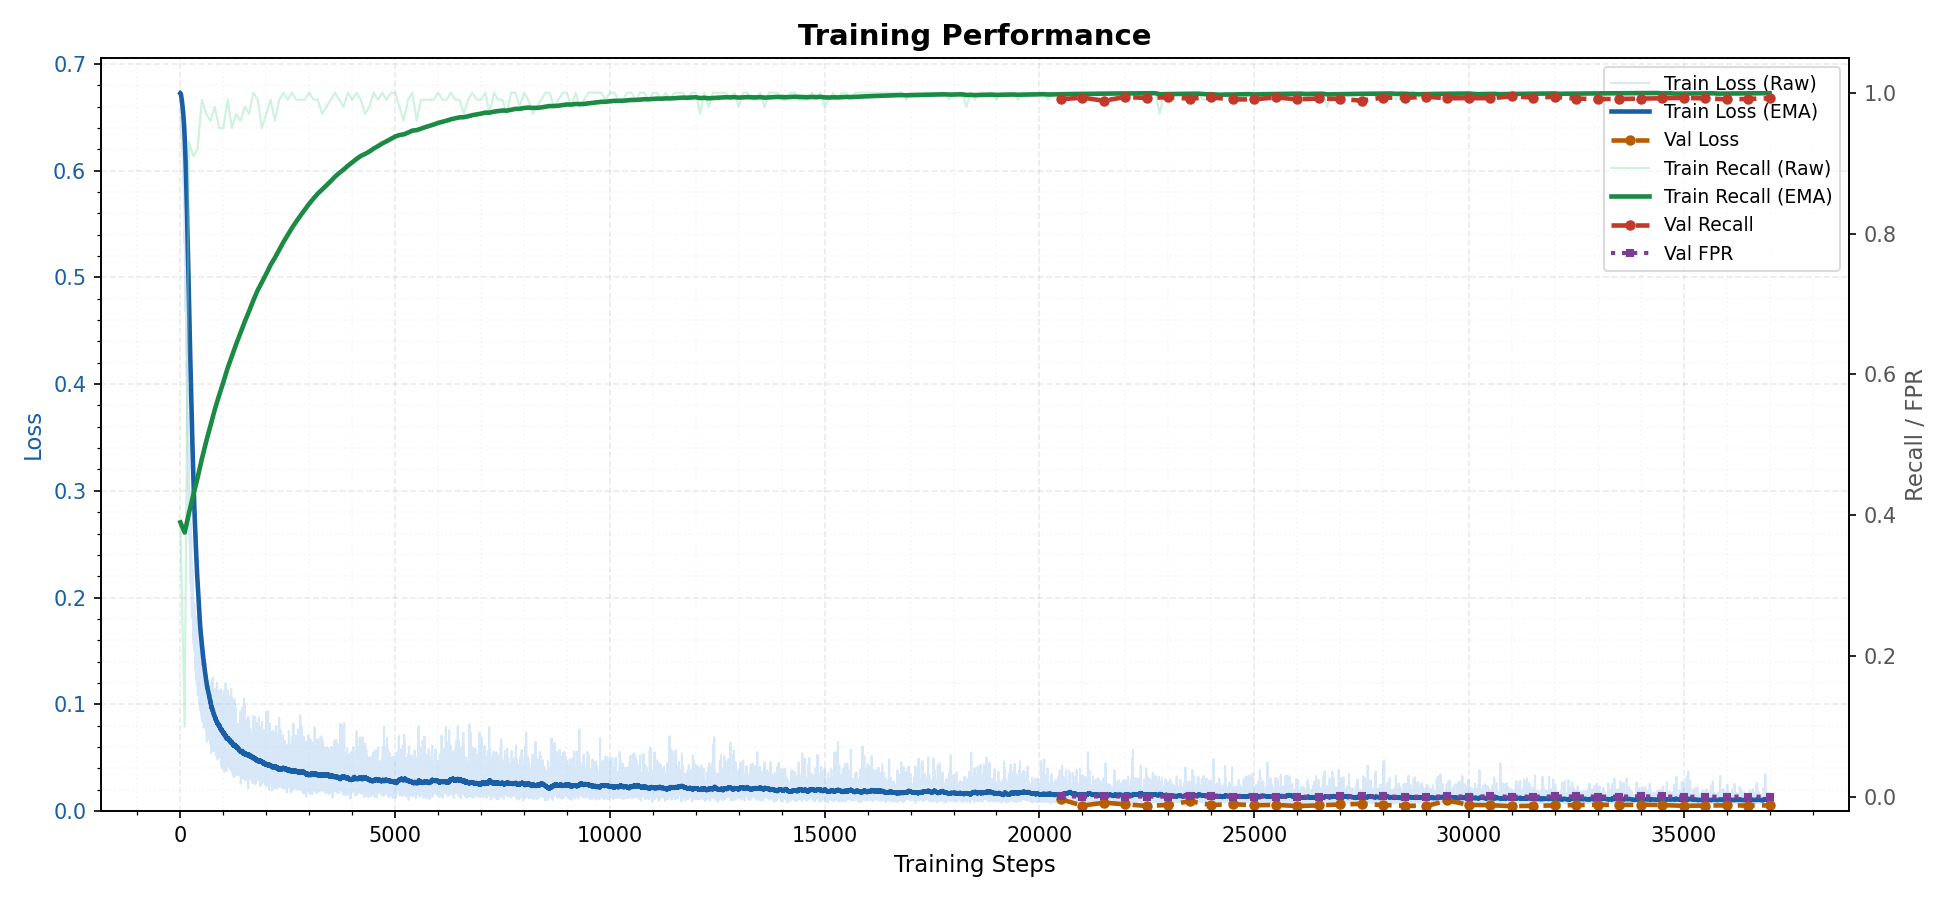
\includegraphics[width=\textwidth,height=0.4\textheight,keepaspectratio]{figures/ch05/training_performance_graph.png}
    \caption{Training Performance Metrics for the custom sanad.onnx Wake Word Model}
    \label{fig:wakeword_training}
\end{figure}

\section{Speech-to-Text (STT) Processing}
Transforming the raw audio of the user's voice into actionable text is handled differently depending on the network state, showcasing the system's hybrid flexibility.

\subsection{The Cloud Pathway (Multimodal Bypass)}
When operating online, the system entirely bypasses traditional STT transcription. Instead of converting speech to text first, the \texttt{llm\_node.py} intercepts the \texttt{audio://} path published by the wakeup node. It reads the raw audio bytes directly from the file system, packages them into a MIME audio object (\texttt{audio/wav}), and attaches it directly to the user's prompt. This payload is sent to Vertex AI's \texttt{gemini-2.5-flash} model, which natively understands audio data alongside text, reducing latency and transcription bottlenecks.

\subsection{The Local Pathway (Whisper \& Hallucination Filtering)}
In offline mode, the system relies on the \texttt{whisper\_node.py} to transcribe the audio into text.
\begin{itemize}
    \item \textbf{Execution:} It invokes a local installation of \texttt{whisper.cpp} (\texttt{whisper-cli}) via a system subprocess, feeding it the temporary WAV file and the optimized quantized model (\texttt{ggml-large-v3-q5\_0.bin}). It also passes the current active language flag (\texttt{-l}) to speed up inference.
    \item \textbf{Bulletproof Filtering:} A known issue with local Whisper models is "hallucination"—where the model invents text or hallucinates phantom subtitles when fed silence or background noise. To combat this, the node implements a strict filter. It drops any transcriptions that consist solely of punctuation and actively scans for a hardcoded list of garbage words (e.g., "Thanks for watching!", "Sous-titres", "شكرا للمشاهدة"). Only clean, validated text is published forward to the Commander node.
\end{itemize}

\section{Dynamic Context Management \& Prompt Engineering}
Before the LLM can make any decisions, it needs a complete, up-to-the-second understanding of the robot's environment and capabilities. This cognitive setup is the primary responsibility of the central orchestrator, \texttt{commander.py}.

\begin{figure}[htbp]
    \centering
    \resizebox{\textwidth}{!}{
    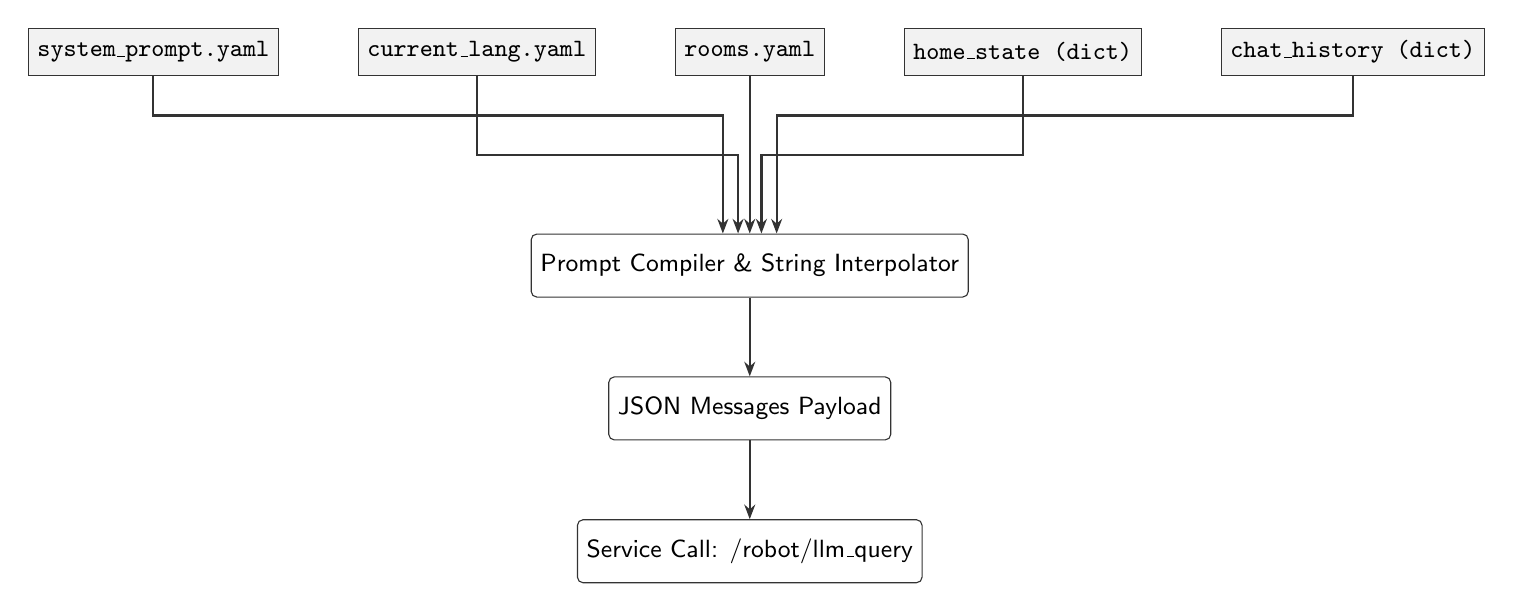
\begin{tikzpicture}[
        node distance=0.5cm and 1cm,
        file/.style={rectangle, draw=black!80, fill=gray!10, minimum height=0.6cm, align=center, font=\ttfamily\small},
        box/.style={rectangle, draw=black!80, fill=white, minimum height=0.8cm, align=center, font=\sffamily\small, rounded corners=2pt},
        arrow/.style={-{Stealth[scale=0.8]}, draw=black!80, thick}
        ]
        
        \node[file] (sys) {system\_prompt.yaml};
        \node[file, right=of sys] (lang) {current\_lang.yaml};
        \node[file, right=of lang] (rooms) {rooms.yaml};
        \node[file, right=of rooms] (state) {home\_state (dict)};
        \node[file, right=of state] (chat) {chat\_history (dict)};
        
        \node[box, below=2cm of rooms] (compiler) {Prompt Compiler \& String Interpolator};
        \node[box, below=1cm of compiler] (payload) {JSON Messages Payload};
        \node[box, below=1cm of payload] (call) {Service Call: /robot/llm\_query};
        
        \draw[arrow] (sys.south) -- ++(0,-0.5) -| (compiler.130);
        \draw[arrow] (lang.south) -- ++(0,-1.0) -| (compiler.110);
        \draw[arrow] (rooms.south) -- (compiler.north);
        \draw[arrow] (state.south) -- ++(0,-1.0) -| (compiler.70);
        \draw[arrow] (chat.south) -- ++(0,-0.5) -| (compiler.50);

        \draw[arrow] (compiler) -- (payload);
        \draw[arrow] (payload) -- (call);
    \end{tikzpicture}
    }
    \caption{Prompt Compilation and Context Injection Mapping}
    \label{fig:s6_context}
\end{figure}

The Commander does not just forward the user's query; it acts as a real-time context compiler, assembling a highly dynamic system prompt before querying the \texttt{/robot/llm\_query} service:

\begin{itemize}
    \item \textbf{Template Resolution:} It begins by loading a base prompt template from \texttt{system\_prompt.yaml}. It immediately replaces static placeholders with dynamic values, such as injecting the \texttt{\{LANGUAGE\_NAME\}} and pulling the current \texttt{\{ROOMS\_LIST\}} directly from the Nav2 \texttt{rooms.yaml} configuration file.
    \item \textbf{State Injection:} The Commander dynamically queries and serializes several critical state variables into JSON format, appending them to the bottom of the system prompt. This includes:
    \begin{itemize}
        \item \textbf{Device States:} The current ON/OFF status of the AC, heater, lights, and TV (\texttt{self.home\_state}).
        \item \textbf{Communication Context:} The names of available Telegram contacts loaded from \texttt{telegram\_contacts.yaml}.
        \item \textbf{Unread Notifications:} Any pending messages waiting in the \texttt{telegram\_messages.yaml} inbox.
    \end{itemize}
    \item \textbf{Conversational Memory (Rolling Window):} To allow for natural, multi-turn conversations (e.g., "Turn on the light," followed by "Actually, turn it off"), the Commander maintains a rolling chat history. It stores the role and content of the last 10 interactions.
\end{itemize}

Finally, the Commander bundles the heavily engineered system prompt together with the rolling chat history and the user's latest command into a single, comprehensive JSON payload, which is then dispatched to the LLM for evaluation.

\section{LLM Reasoning \& Intent Parsing}
Once the LLM (whether cloud-based Gemini or local Qwen) processes the highly contextual system prompt and user command, it must return a response that the robotic system can programmatically understand. It does this by outputting a strictly formatted JSON payload alongside its conversational text.

When the \texttt{llm\_node} returns the AI's response back to the \texttt{commander.py} node, the system runs an extraction routine. The \texttt{extract\_json} method uses regular expressions to strip out extraneous text or reasoning tokens (such as \textless \texttt{think} \textgreater \ tags common in local models) and isolates the core JSON dictionary.

This JSON payload is parsed to determine the user's core intent. The model categorizes the request by generating specific keys such as \texttt{intent}, \texttt{target}, \texttt{action}, \texttt{navigate\_to}, or simply a \texttt{response} string. By inspecting these keys, the system inherently knows whether it needs to control hardware, move to a new location, interact with external APIs, or simply chat with the user.

\section{The Intent Router \& Action Execution}

\begin{figure}[htbp]
    \centering
    \resizebox{\textwidth}{!}{
    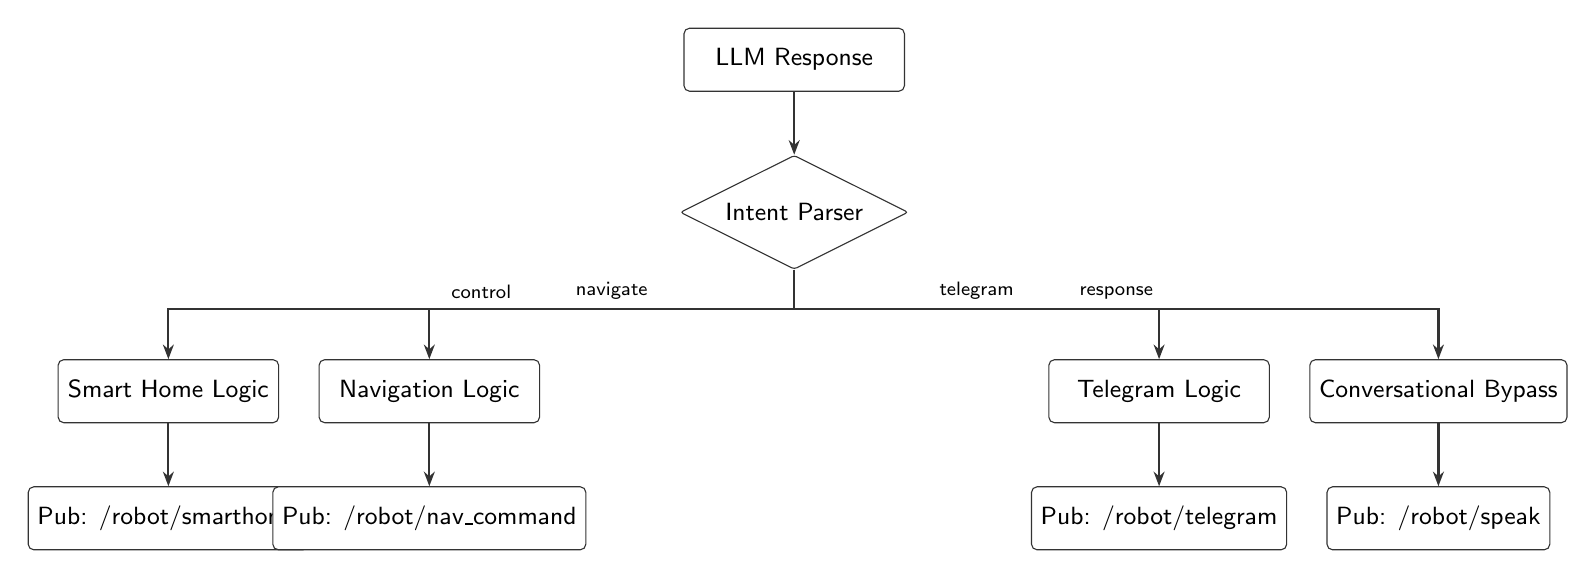
\begin{tikzpicture}[
        node distance=0.8cm and 0.5cm,
        box/.style={rectangle, draw=black!80, fill=white, minimum height=0.8cm, minimum width=2.8cm, align=center, font=\sffamily\small, rounded corners=2pt},
        decision/.style={diamond, aspect=2, draw=black!80, align=center, font=\sffamily\small, rounded corners=1pt},
        arrow/.style={-{Stealth[scale=0.8]}, draw=black!80, thick}
        ]
        
        \node[box] (res) {LLM Response};
        \node[decision, below=of res] (parser) {Intent Parser};
        
        \node[box, below left=1.5cm and 2.5cm of parser] (nav) {Navigation Logic};
        \node[box, left=0.5cm of nav] (sm) {Smart Home Logic};
        
        \node[box, below right=1.5cm and 2.5cm of parser] (tg) {Telegram Logic};
        \node[box, right=0.5cm of tg] (conv) {Conversational Bypass};

        \draw[arrow] (res) -- (parser);
        
        \draw[arrow] (parser.south) -- ++(0,-0.5) -| node[pos=0.25, above, font=\sffamily\scriptsize] {control} (sm.north);
        \draw[arrow] (parser.south) -- ++(0,-0.5) -| node[pos=0.25, above, font=\sffamily\scriptsize] {navigate} (nav.north);
        \draw[arrow] (parser.south) -- ++(0,-0.5) -| node[pos=0.25, above, font=\sffamily\scriptsize] {telegram} (tg.north);
        \draw[arrow] (parser.south) -- ++(0,-0.5) -| node[pos=0.25, above, font=\sffamily\scriptsize] {response} (conv.north);

        \node[box, below=of sm] (pubsm) {Pub: /robot/smarthome};
        \node[box, below=of nav] (pubnav) {Pub: /robot/nav\_command};
        \node[box, below=of tg] (pubtg) {Pub: /robot/telegram};
        \node[box, below=of conv] (pubtts) {Pub: /robot/speak};

        \draw[arrow] (sm) -- (pubsm);
        \draw[arrow] (nav) -- (pubnav);
        \draw[arrow] (tg) -- (pubtg);
        \draw[arrow] (conv) -- (pubtts);
    \end{tikzpicture}
    }
    \caption{ROS 2 Intent Demultiplexer and Topic Routing}
    \label{fig:s8_router}
\end{figure}

The \texttt{commander.py} node serves as the central switchboard, taking the parsed JSON dictionary and distributing the commands to the appropriate ROS 2 subsystems.

\subsection{Smart Home Control}
If the JSON dictionary contains an \texttt{intent} labeled \texttt{control} or a dedicated \texttt{controls} list, the router targets the IoT devices.
\begin{itemize}
    \item It extracts the \texttt{target} (e.g., "ac", "light", "tv") and the desired \texttt{action} (e.g., "on", "off").
    \item Before commanding the hardware, the Commander updates its internal \texttt{self.home\_state} dictionary to reflect the new status (e.g., changing the AC state to 'on'). This ensures the LLM knows the device is already on during the next conversation turn.
    \item Finally, the routing logic publishes the control array as a JSON string to the \texttt{/robot/smarthome\_command} topic for the hardware actuators to execute.
\end{itemize}

\subsection{Autonomous Navigation}
When the user asks the robot to move, the LLM includes a \texttt{navigate\_to} key in its JSON output.
\begin{itemize}
    \item The Commander dynamically reloads the system's spatial coordinates from the \texttt{rooms.yaml} file to ensure it has the most up-to-date map data.
    \item It matches the requested room name to its precise X, Y, and Z pose coordinates.
    \item The router then publishes the movement intent to the \texttt{/robot/nav\_command} topic. Simultaneously, it initiates an asynchronous service call to the \texttt{rooms/navigate} Nav2 endpoint, which physically commands the robot's drive base to travel to the destination.
\end{itemize}

\subsection{Asynchronous Communication (Telegram)}
The Commander can seamlessly interface with external messaging services by parsing specific Telegram intents.
\begin{itemize}
    \item \textbf{Sending Messages:} If the intent is \texttt{telegram}, the system extracts the \texttt{contact} name and the \texttt{message} text. It verifies the contact against the dynamically loaded \texttt{telegram\_contacts.yaml} database. If a match is found, it publishes the payload to the \texttt{/robot/telegram/send} topic, where the dedicated \texttt{telegram\_node.py} handles the API web request.
    \item \textbf{Reading/Clearing Notifications:} If the intent is \texttt{read\_telegram}, the Commander determines the scope (either clearing all messages or just messages from a specific sender) and publishes a clear command to the \texttt{/robot/telegram/clear} topic, which updates the local inbox file.
\end{itemize}

\subsection{The Conversational Bypass}
Not every user interaction requires a physical action. If the user asks a general knowledge question ("How do car gears work?") or requests a recipe, the LLM will generate a JSON payload lacking movement or control intents, featuring only the \texttt{response} key.
\begin{itemize}
    \item The Commander extracts this \texttt{response} string.
    \item It completely bypasses all the hardware action routers and publishes the text directly to the \texttt{/robot/speak} topic.
    \item This triggers the TTS node to vocalize the response, creating a seamless conversational experience where the robot acts as a pure knowledge assistant in the user's spoken language.
\end{itemize}

\section{Text-to-Speech (TTS) Synthesis}
The final stage of the Sanad voice pipeline is the \texttt{tts\_node.py}, which is responsible for giving the robot a voice. It constantly listens to the \texttt{/robot/speak} topic for text payloads dispatched by the Commander node. To ensure the robot's voice is responsive and natural, the node implements two distinct playback strategies depending on the network availability.

\begin{figure}[htbp]
    \centering
    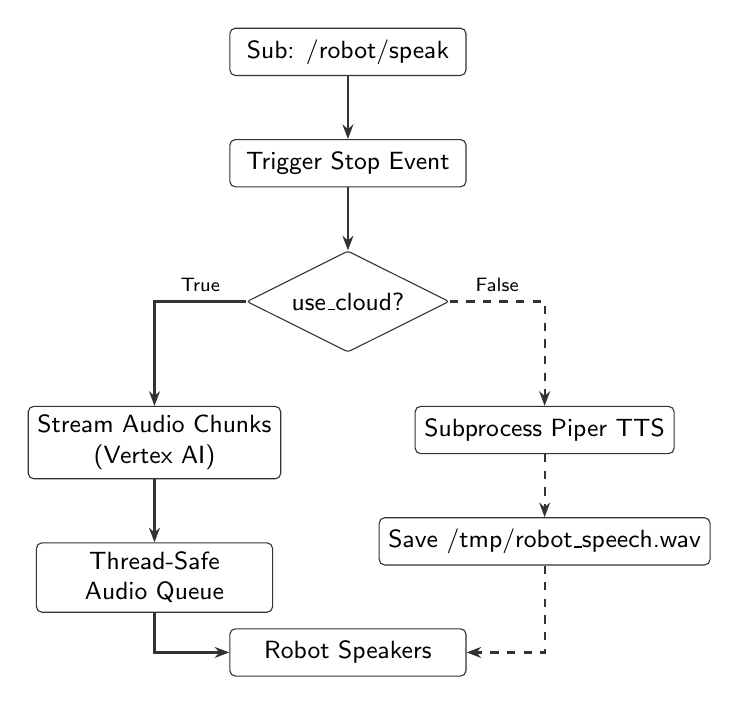
\begin{tikzpicture}[
        node distance=0.8cm and 2cm,
        box/.style={rectangle, draw=black!80, fill=white, minimum height=0.6cm, minimum width=3cm, align=center, font=\sffamily\small, rounded corners=2pt},
        decision/.style={diamond, aspect=2, draw=black!80, align=center, font=\sffamily\small, rounded corners=1pt},
        arrow/.style={-{Stealth[scale=0.8]}, draw=black!80, thick},
        dashedarrow/.style={-{Stealth[scale=0.8]}, draw=black!80, thick, dashed}
        ]
        
        \node[box] (sub) {Sub: /robot/speak};
        \node[box, below=of sub] (stop) {Trigger Stop Event};
        \node[decision, below=of stop] (cloud) {use\_cloud?};
        
        \node[box, below left=1cm and 0.2cm of cloud] (stream) {Stream Audio Chunks\\(Vertex AI)};
        \node[box, below right=1cm and 0.2cm of cloud] (piper) {Subprocess Piper TTS};
        
        \node[box, below=of stream] (q) {Thread-Safe\\Audio Queue};
        \node[box, below=of piper] (wav) {Save /tmp/robot\_speech.wav};

        \node[box, below=3.5cm of cloud] (spk) {Robot Speakers};

        \draw[arrow] (sub) -- (stop);
        \draw[arrow] (stop) -- (cloud);
        
        \draw[arrow] (cloud.west) -| node[above, near start, font=\sffamily\scriptsize] {True} (stream.north);
        \draw[dashedarrow] (cloud.east) -| node[above, near start, font=\sffamily\scriptsize] {False} (piper.north);
        
        \draw[arrow] (stream) -- (q);
        \draw[dashedarrow] (piper) -- (wav);
        
        \draw[arrow] (q.south) |- (spk.west);
        \draw[dashedarrow] (wav.south) |- (spk.east);
    \end{tikzpicture}
    \caption{Hybrid Text-to-Speech Synthesis and Audio Buffering}
    \label{fig:s9_tts}
\end{figure}

\subsection{The Cloud Pathway (Real-Time Streaming)}
When the system operates online, it connects to Google Cloud's Vertex AI using the \texttt{gemini-2.5-flash-preview-tts} model.
\begin{itemize}
    \item To drastically reduce latency, the system employs a streaming architecture rather than waiting for the entire response to be synthesized.
    \item The node's \texttt{AudioPlayer} class opens a continuous \texttt{sounddevice} output stream in a background thread.
    \item As the cloud API returns individual audio chunks, the system intercepts the raw PCM bytes, dynamically resamples them via linear interpolation (from the input rate of 24,000 Hz to the system output rate of 44,100 Hz), and pushes them into a playback queue.
    \item This allows the robot to begin speaking the first words of a sentence while the rest of the paragraph is still being generated on the server.
\end{itemize}

\subsection{The Local Pathway (Offline Synthesis)}
In offline mode, the node gracefully falls back to a local Piper TTS engine.
\begin{itemize}
    \item It executes a subprocess that calls the \texttt{piper} binary, feeding it the text alongside a local ONNX voice model (such as \texttt{ar\_JO-kareem-medium.onnx}).
    \item Unlike the cloud's chunked streaming, the local Piper execution generates a complete, temporary WAV file (\texttt{/tmp/robot\_speech.wav}).
    \item Once the synthesis is finished, the \texttt{AudioPlayer} reads the file using the \texttt{soundfile} library and plays it synchronously through the speakers.
\end{itemize}

\subsection{Interrupt \& Audio Management}
Regardless of whether the TTS is streaming from the cloud or playing a local WAV file, the node features robust audio thread management. The \texttt{AudioPlayer} class utilizes threading events (\texttt{stop\_event}) to track the playback state. If the robot is in the middle of speaking a long paragraph and the user issues a new command, the TTS node will instantly trigger the stop event, close the audio stream, drain the playback queue, and prepare to speak the newly generated response.

\section{Summary and Transition}
This chapter has detailed the hybrid voice control interface, explaining how spoken Arabic commands are parsed into system goals. The next chapter, Chapter 6 (Server Architecture and Design), describes the Node.js integration server that bridges these external client interfaces with the core ROS 2 message system.

\chapterseparator{Chapter 6}
\setcounter{chapter}{6}
\chapter*{Chapter (6): SERVER ARCHITECTURE AND DESIGN}
\addcontentsline{toc}{chapter}{Chapter (6): Server Architecture and Design}
\setcounter{section}{0}


\section{Chapter Preview}
\label{sec:ch8_intro}
This chapter presents the design and implementation of the central Node.js integration server. It details the server's role as a non-invasive, SCADA-like supervisory layer that translates client HTTP/WebSocket protocols, aggregates ROS bridge topics, and exposes modules for smart-home control and caregiver communications.

\subsection{Problem Context}
\label{sec:ch8_problem}

The robotic platform developed in this study is predicated on the Robot Operating System (ROS), which inherently provides the necessary infrastructure for internal orchestration, encompassing node-to-node communication, topic publication and subscription, and service calls among the system's internal modules. While ROS is highly optimized for coordinating tightly coupled robotic processes, it is not inherently designed to interface directly with external heterogeneous clients. Such clients include end-user mobile applications, remote interaction interfaces (e.g., Telegram clients), and third-party smart-home peripherals utilizing standard network protocols rather than native ROS messages.

Integrating HTTP communication directly into ROS nodes, or embedding web-server logic within them, would inadvertently couple the release cycles of user-facing features with the core robotics stack. Consequently, minor modifications to mobile-facing functionalities would necessitate concurrent testing and deployment of motion control, navigation, and sensor processing modules, despite their logical independence. To mitigate this tight coupling, the dedicated server architecture detailed in this chapter was developed.

\subsection{Design Goals}
\label{sec:ch8_goals}

The architectural decisions presented in this chapter are guided by four primary objectives:

\begin{itemize}
    \item \textbf{Non-invasiveness} — The server must supplement rather than replace or duplicate the native orchestration logic of ROS. It functions as an observer and forwarder, without dictating autonomous robotic behavior.
    \item \textbf{Modularity} — Novel capabilities (e.g., additional smart-home device protocols, new remote commands) must be integrated as self-contained modules to avoid structural modifications to unrelated components.
    \item \textbf{Operability} — The system must demonstrate resilience and predictable recovery during operational failures, particularly connection disruptions with \texttt{rosbridge}, avoiding silent failures or the necessity for manual intervention.
    \item \textbf{Developer Ergonomics} — To facilitate future maintainability and extensibility, the codebase prioritizes self-explanatory design patterns over excessive terseness, ensuring accessibility for subsequent developers.
\end{itemize}

\subsection{Architectural Analogy to SCADA Systems}
\label{sec:ch8_scada}

To provide a clear conceptual model for engineering professionals, the proposed server architecture can be functionally mapped to a Supervisory Control and Data Acquisition (SCADA) topology. While the implemented system does not adhere to stringent industrial determinism or standards, it adopts a structurally analogous multi-tiered approach to decouple real-time hardware control from user-facing interfaces.

This functional similarity is primarily observed in the stratification of system responsibilities, as summarized in Table~\ref{tab:scada_mapping}.

\begin{table}[H]
    \centering
    \caption{Functional mapping of the project architecture to standard SCADA layers.}
    \begin{tabular}{|l|l|p{6cm}|}
        \hline
        \textbf{SCADA Layer} & \textbf{Project Component} & \textbf{Functional Responsibility} \\
        \hline
        Field / Control Layer & ROS (Robot Operating System) & Direct, real-time actuation and sensory data acquisition. \\
        \hline
        Supervisory Layer & Custom Node.js Server & Protocol translation, data aggregation, and routing between hardware and clients. \\
        \hline
        Presentation Layer (HMI) & Mobile App \& Telegram Client & High-level operator observation and command issuance, abstracted from underlying field protocols. \\
        \hline
    \end{tabular}

    \label{tab:scada_mapping}
\end{table}

By conceptualizing the server as a supervisory translator, the architecture achieves a modular separation of concerns. This ensures that the presentation layer remains insulated from the complexities of the robotics middleware, facilitating independent scalability and maintenance across the communication stack.

\section{Architectural Evolution}
\label{sec:ch8_evolution}

With the motivating context and design goals established in Section~\ref{sec:ch8_intro}, this section traces the iterative structural refinements that shaped the server's current form. Each transition is presented in chronological order and emerged as a direct resolution to a concrete operational challenge encountered during development.

\subsection{First Iteration: Layered Architecture}
\label{sec:ch8_layered}

The initial server implementation adopted a conventional horizontal layered architecture. The codebase was segregated by technical function: a global \texttt{routes} directory for endpoint definitions, \texttt{controllers} for request handling, \texttt{services} for business logic, and \texttt{models} for data persistence. While theoretically separating concerns, this structure proved suboptimal as the feature set expanded.

Developing or modifying a single feature, such as infrared (IR) remote control, necessitated navigating four distinct files across disparate directories (e.g., \texttt{ir.routes.js}, \texttt{ir.controller.js}, \texttt{ir.service.js}, \texttt{ir.model.js}). This fragmented organization imposed a high cognitive load, which escalated as additional features (smart home integration, telemetry endpoints, navigation) were introduced. The directory-based navigation paradigm effectively deteriorated, prompting a structural paradigm shift.

\subsection{Second Iteration: Feature-Based Modular Architecture}
\label{sec:ch8_feature_based}

To address the limitations of the horizontal structure, the organizing principle was transitioned to a feature-centric modular architecture. The application was compartmentalized such that each feature (e.g., IR, Telegram, room management) resided in a self-contained directory containing its specific routes, controllers, Data Transfer Objects (DTOs), and business logic. Cross-cutting concerns, such as authentication middleware and global error handlers, were abstracted into a shared core layer.

This reorganization significantly improved development efficiency. Feature encapsulation ensured that modifications were localized, and new functionalities could be modeled after existing modules without the overhead of distributing logic across technical layers. This architecture proved highly scalable for an expanding feature set.

\subsection{The Controller Overcrowding Problem}
\label{sec:ch8_overcrowding}

Despite the improvements in module organization, individual controller functions progressively exhibited excessive responsibilities. Prior to subsequent refinements, a typical controller handled four distinct tasks:

\begin{itemize}
\item Manual validation of incoming request payloads to ensure structural and typological correctness.
    \item Execution of core business logic.
    \item Exception handling and categorization of errors into appropriate HTTP status codes.
    \item Formatting and transmission of standard JSON responses.
\end{itemize}

This aggregation of concerns is a recognized anti-pattern in scalable service design. The manual replication of error-handling and response-formatting logic across controllers increased the probability of inconsistent API responses and systemic bugs, complicating the development of robust client-side error handling.

\subsection{The Controller Wrapper Pattern}
\label{sec:ch8_wrapper}

To resolve the overcrowding identified in Section~\ref{sec:ch8_overcrowding}, error handling and response formatting were abstracted into a centralized wrapper function. Every controller is passed through this wrapper prior to its registration as an Express route handler.

Under this paradigm, the controller's contract is strictly limited: it must return a valid output upon success or throw an exception upon failure. The controller contains no HTTP-specific constructs (e.g., status codes or response objects). The wrapper assumes full responsibility for HTTP semantics, catching exceptions, assigning appropriate status codes, standardizing error payloads, and enveloping successful responses. This separation of concerns structurally guarantees consistency across the entire API surface.

\subsection{Global Error Handler}
\label{sec:ch8_error_handler}

Complementing the wrapper, the controller wrapper delegates caught exceptions to a global error handler middleware via the \texttt{next(err)} function. This architectural decision decouples error interception from error resolution, allowing the global middleware to handle logging, environment-specific stack trace obfuscation, and final response dispatching autonomously.

\subsection{Input Validation with Zod}
\label{sec:ch8_zod}

The centralization strategy was subsequently applied to request validation. Manual validation logic within controllers was replaced by declarative schema validation using the Zod library. Each route is associated with a specific DTO schema. Incoming requests are evaluated against the corresponding DTO at the routing layer; malformed requests are intercepted and rejected prior to controller invocation.

Consequently, controllers operate under the strict assumption of type-safe and structurally validated inputs. This elimination of defensive programming within business logic further purifies the controller's responsibility, ensuring it focuses exclusively on feature execution.

\subsection{From Manual Router Wiring to Declarative Route Configuration}
\label{sec:ch8_declarative}

The final architectural refinement addressed the inefficiencies of imperative route wiring. Traditional configuration entails manually binding paths, middleware, and controllers (e.g., \texttt{router.get(...)}), which becomes cumbersome and error-prone as the API surface expands.

This approach was superseded by a declarative route registry. Feature modules now export a structured route table comprising route descriptors. Each descriptor is a plain configuration object whose parameters define the route's identity, behavior, and middleware requirements. Figure~\ref{fig:route_config} illustrates the abstract structure of this descriptor and the configuration parameters available to each route entry.

During initialization, a unified \texttt{attachRoutesAndMiddlewares} function iterates over these descriptor tables. It dynamically composes the middleware pipeline—applying DTO validation (Section~\ref{sec:ch8_zod}), authentication, and the controller wrapper (Section~\ref{sec:ch8_wrapper})—and binds the resulting chain to the Express application instance.

\begin{figure}[H]
    \centering
    \includegraphics[width=0.8\textwidth]{"figures/ch06/sanad - Page 1 aggragator configurations(1).png"}
    \caption{Abstract route descriptor object and its configuration parameters.}
    \label{fig:route_config}
\end{figure}

This methodology yields three significant advantages:

\begin{enumerate}
    \item \textbf{Self-Documentation:} The route table acts as an accessible API manifest, enhancing code readability and maintainability.
    \item \textbf{Structural Consistency:} Critical middlewares (validation, error wrapping) are systematically applied by the registry, eliminating the risk of developer omission.
    \item \textbf{Flexibility:} A \texttt{customRouter} parameter permits the instantiation of conventional Express routers for edge cases that preclude declarative definition.
\end{enumerate}

As a concrete example, the IR module's declarative configuration resolves to the deterministic API surface shown in Table~\ref{tab:ir_routes}.

\begin{table}[H]
    \centering
    \caption{Resolved IR module API surface.}
    \begin{tabular}{|l|l|l|}
        \hline
        \textbf{Method} & \textbf{Path} & \textbf{Purpose} \\
        \hline
        GET & \texttt{/api/v1/ir/device} & Retrieve a specific registered IR device \\
        \hline
        GET & \texttt{/api/v1/ir/devices} & Retrieve the collection of all IR devices \\
        \hline
    \end{tabular}
    \label{tab:ir_routes}
\end{table}

\subsection{Reflection on the Evolution}
\label{sec:ch8_reflection}

The successive architectural transitions share a unified objective: abstracting cross-cutting concerns from individual feature logic into centralized, deterministic mechanisms. The shift to feature-based modularity optimized navigation; the controller wrapper standardized response semantics; DTO validation ensured input integrity; and declarative routing systematized endpoint configuration. These enhancements collectively fortified the system's robustness without compromising its functional capabilities. The resulting architecture is presented in its finalized form in the following section.

\section{System Architecture Overview}
\label{sec:ch8_system_arch}

Building upon the evolutionary refinements documented in Section~\ref{sec:ch8_evolution}, this section presents the finalized system architecture. Figure~\ref{fig:system_arch} provides a comprehensive view of the server's structural composition and the communication pathways between its principal components.

\begin{figure}[H]
    \centering
    \includegraphics[width=0.8\textwidth]{"figures/ch06/sanad - Page 1 system arch.png"}
    \caption{Comprehensive system architecture.}
    \label{fig:system_arch}
\end{figure}

\subsection{Server Builder and the Dual-Server Model}
\label{sec:ch8_dual_server}

As depicted in Figure~\ref{fig:system_arch}, the high-level architecture is orchestrated by a central \texttt{server builder}, which instantiates two concurrent server processes within the same execution context: an \texttt{expressServer} for stateless RESTful interactions and a \texttt{wsServer} for persistent, bidirectional WebSocket communications.

The Express server interfaces with the API aggregator (detailed in Section~\ref{sec:ch8_aggregator}), which serves as the unified entry point for HTTP-based modules (e.g., IR control, Telegram integration, telemetry). Conversely, the WebSocket server is architecturally isolated and explicitly designated for high-frequency robotic motion control commands.

\subsection{Rationale for Server Separation}
\label{sec:ch8_separation}

The bifurcation of REST and WebSocket servers is predicated on the fundamentally disparate communication paradigms they serve. REST architectures utilize a request/response model suitable for discrete queries. In contrast, motion control necessitates a low-latency, continuous telemetry stream where the overhead of establishing successive HTTP connections is prohibitive. Providing dedicated transport channels for these distinct modalities ensures optimal network utilization and minimizes latency for real-time robotic actuation.

\section{API Aggregator}
\label{sec:ch8_aggregator}

Having established the dual-server model in Section~\ref{sec:ch8_dual_server}, this section examines the internal composition of the Express server's central routing mechanism. Figure~\ref{fig:api_aggregator} illustrates the aggregator's layered pipeline.

\begin{figure}[H]
    \centering
    \includegraphics[width=0.8\textwidth]{"figures/ch06/sanad - Page 1 API aggregator.png"}
    \caption{Internal structure of the API Aggregator.}
    \label{fig:api_aggregator}
\end{figure}

The API aggregator functions as the central conduit exposing the server's feature modules to external clients. It leverages the \texttt{routerRegistry} to systematically apply five distinct layers to incoming requests:

\begin{itemize}
    \item \textbf{Endpoints} — The configured route table defining the API schema (Section~\ref{sec:ch8_declarative}).
    \item \textbf{Input Validation} — Zod DTO schemas for request sanitization (Section~\ref{sec:ch8_zod}).
    \item \textbf{Authenticator} — JWT-based middleware for access control (Section~\ref{sec:ch8_auth}).
    \item \textbf{Middlewares} — Route-specific interceptors (e.g., rate limiting).
    \item \textbf{Controller Wrapper} — The centralized exception-handling and response-formatting layer (Section~\ref{sec:ch8_wrapper}).
\end{itemize}

\subsection{Authentication Strategy}
\label{sec:ch8_auth}

Authentication is governed by a stateless JSON Web Token (JWT) mechanism rather than stateful, session-backed architectures. This approach is highly compatible with heterogeneous client environments (e.g., mobile applications and remote Telegram instances), as the JWT encapsulates cryptographic proof of validity without necessitating continuous database lookups.


\subsection{Controller Wrapper Internals}
\label{sec:ch8_wrapper_internals}

As introduced in Section~\ref{sec:ch8_wrapper}, the controller wrapper isolates two critical operational phases:

\begin{itemize}
    \item \textbf{Exception Interception}: Maps internal exceptions to standard HTTP status codes and uniform error payloads.
    \item \textbf{Response Construction}: Standardizes the structural envelope (e.g., a standard \texttt{{ data: ... }} JSON object) for successful executions.
\end{itemize}

This decoupling ensures that error-handling logic remains completely agnostic to success-formatting requirements, thereby facilitating independent maintenance and reducing code fragility.

\section{ROS Bridge Integration Layer}
\label{sec:ch8_rosbridge}

The preceding sections addressed the server's HTTP-facing architecture. This section shifts focus to the opposing interface: the connection between the server and the ROS infrastructure it mediates. All ROS-facing communication is channeled through a dedicated integration layer built on \texttt{rosbridge}.

\subsection{The Shared Connection Model}
\label{sec:ch8_shared_conn}

Interactions with the underlying ROS infrastructure are multiplexed through a singular, shared \texttt{rosbridge} connection object, rather than permitting feature modules to instantiate independent sockets. Centralization is imperative for reliable fault tolerance. If individual modules maintained distinct connections, a localized network disruption could result in silent failures, wherein a module retains a reference to a defunct connection without triggering a systemic error cascade.

\subsection{Reconnection Strategy}
\label{sec:ch8_reconnect}

To address potential connectivity loss, the integration layer monitors the \texttt{rosbridge} client for \texttt{reconnect} events. Upon connection restoration, the system deliberately eschews selective revalidation of existing communication pipelines. Instead, it executes a comprehensive teardown of all active subscribers, publishers, and service clients, subsequently re-instantiating them against the newly established connection object. This lifecycle is illustrated in Figure~\ref{fig:rosbridge}.

\begin{figure}[H]
    \centering
    \includegraphics[width=0.8\textwidth]{"figures/ch06/rosbridge image.png"}
    \caption{ROS bridge WebSocket connection lifecycle.}
    \label{fig:rosbridge}
\end{figure}

\subsection{Trade-offs of Comprehensive Rebuilding}
\label{sec:ch8_rebuild_tradeoff}

The decision to unconditionally rebuild the communication topology represents a deliberate engineering trade-off. While implementing differential patching—rebuilding only definitively broken instances—might yield marginal runtime efficiencies, it necessitates complex state-tracking mechanisms for every active pipeline. Inaccuracies in such tracking often manifest as silent operational failures in production.

The comprehensive rebuild strategy guarantees deterministic recovery through a unified teardown-and-initialization sequence. The minor overhead incurred by re-instantiating functional objects is considered an acceptable compromise to ensure systemic reliability and mitigate extensive debugging costs associated with partial state corruption. This design directly addresses the operability goal established in Section~\ref{sec:ch8_goals}.

\section{Feature Modules}
\label{sec:ch8_features}

The architectural foundations described in Sections~\ref{sec:ch8_evolution} through~\ref{sec:ch8_rosbridge} provide the shared infrastructure upon which individual feature modules are built. This section examines three representative modules—IR remote control, smart home integration, and Telegram client integration—each of which illustrates how the modular architecture accommodates distinct communication patterns and external device protocols.

\subsection{IR Remote Control}
\label{sec:ch8_ir}

\subsubsection{Device Registration Protocol}
\label{sec:ch8_ir_registration}

The integration of new infrared (IR) remotes necessitates a robust registration protocol to mitigate hardware-induced signal noise. Figure~\ref{fig:ir_sequence} presents the sequence diagram for this process.

\begin{figure}[H]
    \centering
    \includegraphics[width=0.8\textwidth]{"figures/ch06/sanad - Page 1 IR.png"}
    \caption{IR device registration sequence diagram.}
    \label{fig:ir_sequence}
\end{figure}

The mobile client initiates a registration session, which the server tracks contextually. Concurrently, the ROS infrastructure monitors physical button actuations, publishing detected hex codes to the \texttt{/ir/hexCode} topic. The server evaluates these emissions as \textit{candidate} keys, withholding database persistence to preclude the recording of corrupted signals.

Subsequently, the client application retrieves the candidate key and issues an explicit confirmation request. Upon successful verification, the server invokes the ROS \texttt{/ir/fullDevice} service to finalize the profile. This two-phase commit protocol—capture followed by explicit confirmation—ensures that transient signal corruption does not compromise the integrity of the device's persistent key mapping.

\subsection{Smart Home Integration}
\label{sec:ch8_smarthome}

While the IR module interfaces with ROS-connected hardware, the smart home subsystem extends the server's reach to network-connected peripherals operating independently of the robotics stack. This module addresses two distinct challenges: peripheral discovery and unified command dispatch.

\subsubsection{Discovery Protocol}
\label{sec:ch8_discovery}

The integration of smart-home peripherals utilizes a dynamic, broadcast-based auto-discovery mechanism, obviating the need for static IP configuration. The discovery phase is depicted in Figure~\ref{fig:discovery_stage}, with the detailed broadcast and self-announcement flow shown in Figure~\ref{fig:discovery_flow}.

\begin{figure}[H]
    \centering
    \includegraphics[width=0.8\textwidth]{"figures/ch06/discovery stage.png"}
    \caption{Smart home peripheral discovery phase.}
    \label{fig:discovery_stage}
\end{figure}

\begin{figure}[H]
    \centering
    \includegraphics[width=0.8\textwidth]{"figures/ch06/sanad - Page 1 smart home discovery.png"}
    \caption{Smart home broadcast and self-announcement flow.}
    \label{fig:discovery_flow}
\end{figure}

The server periodically transmits discovery beacons across the local network. Compatible peripherals intercept these broadcasts and respond with their control typologies and unique identifiers, allowing the server to autonomously register them. This methodology mirrors established zero-configuration networking protocols (e.g., mDNS, SSDP) and is essential in robotics deployments where the environmental topology is highly variable, facilitating seamless hardware integration without manual supervisory intervention.

\subsubsection{Unified Control Architecture}
\label{sec:ch8_unified_control}

A key architectural decision in this module is the normalization of actuation commands regardless of their origin. As illustrated in Figure~\ref{fig:control_path}, both human operators (via the mobile application) and autonomous processes (via ROS) interface with a unified server layer, which subsequently routes the command to the target peripheral.

\begin{figure}[H]
    \centering
    \includegraphics[width=0.8\textwidth]{"figures/ch06/server-control.png"}
    \caption{Unified control pathway for smart home devices.}
    \label{fig:control_path}
\end{figure}

This centralization prevents the duplication of control logic. Without a unified interface, integration of a new peripheral would require parallel implementations for both manual and autonomous control pathways, increasing maintenance complexity. By converging these pathways at the server level, a peripheral requires only a single integration point to become accessible to both human operators and autonomous robotic routines.

The underlying data model supporting this integration is depicted in Figure~\ref{fig:smarthome_schema}.

\begin{figure}[H]
    \centering
    \includegraphics[width=0.8\textwidth]{"figures/ch06/smart-home-db-schema.png"}
    \caption{Entity-relationship schema for smart-home integration.}
    \label{fig:smarthome_schema}
\end{figure}

\subsection{Telegram Client Integration}
\label{sec:ch8_telegram}

The final feature module examined in this chapter provides remote access to the robotic platform via the Telegram messaging service. Unlike the preceding modules, which communicate over local network protocols, the Telegram integration introduces challenges related to external session management and cross-channel authentication.

\subsubsection{Connection and Session Lifecycle}
\label{sec:ch8_telegram_session}

Upon initialization of a Telegram interaction, the system evaluates the persistence of an existing, valid session for the corresponding user, as depicted in Figure~\ref{fig:telegram_session}. If no valid session is detected, a novel connection protocol is initiated. If a session is available, the workflow transitions directly to the authentication phase managed by the OTP manager (Section~\ref{sec:ch8_otp}).

\begin{figure}[H]
    \centering
    \includegraphics[width=0.8\textwidth]{"figures/ch06/sanad - Page 1 telegram connection.png"}
    \caption{Telegram connection and session orchestration flow.}
    \label{fig:telegram_session}
\end{figure}

This session validation is critical for operational efficiency. Establishing a Telegram client connection from scratch is computationally and experientially expensive, often necessitating full OTP re-verification. Exploiting cached session states circumvents redundant authentication cycles, thereby significantly enhancing the user experience by maintaining uninterrupted connectivity.


\subsubsection{OTP Manager and Asynchronous Resolution}
\label{sec:ch8_otp}

The OTP manager addresses a fundamental challenge in cross-channel authentication: synchronizing two events that occur on entirely independent communication pathways at unpredictable times. Its architecture, shown in Figure~\ref{fig:otp_manager}, employs a two-promise resolution pattern to bridge this temporal gap.

\begin{figure}[H]
    \centering
    \includegraphics[width=0.8\textwidth]{"figures/ch06/sanad - Page 1 OTP manager.png"}
    \caption{Two-promise resolution architecture of the OTP manager.}
    \label{fig:otp_manager}
\end{figure}

Initiation of an authentication \texttt{Request} generates two corresponding entries: a \textbf{pending session} state and a \textbf{pending OTP} state. The requisite OTP is subsequently provided by the user via the Telegram interface—an asynchronous event received on an orthogonal system entry point. Upon validation of the provided OTP, the pending OTP entry is resolved, which sequentially triggers the resolution of the interdependent pending session.

This architectural decoupling is imperative due to the asynchronous nature of the Telegram protocol. The originating authentication process cannot synchronously block while awaiting user input via the Telegram bot. The promise-resolution pattern bridges this temporal and spatial gap, enabling the originating request to resolve deterministically based on input received from an entirely distinct interaction pathway.

\section{Summary and Transition}
\label{sec:ch8_conclusion}
This chapter has detailed the Node.js supervisory server, demonstrating how it securely handles client requests, aggregates diagnostics, and manages asynchronous peripherals. The next chapter, Chapter 7 (Touchscreen Interface), describes the development of the primary on-board kiosk UI that consumes these server APIs.

\chapterseparator{Chapter 7}
\setcounter{chapter}{7} 
\chapter*{Chapter (7): Touchscreen Interface}
\addcontentsline{toc}{chapter}{Chapter (7): Touchscreen Interface} 
\renewcommand{\thesection}{\thechapter.\arabic{section}}
\setcounter{section}{0}
\captionsetup[figure]{justification=centering}


\section{Chapter Preview}
This chapter covers the design and implementation of the on-board touchscreen human-machine interface (HMI). It outlines the functional and usability requirements, explains the Preact and Vite technology stack selection, details the application components and WebSocket-based ROS 2 communication, and presents the accessibility design features.

To support these diverse needs, the interface must satisfy a rigorous set of functional and non-functional requirements. The core design principles are simplicity, high visibility, and error-prevention. Since the user may operate the system in motion or under cognitive fatigue, touch targets must be large and forgiving, and system states must be obvious. Table \ref{tab:kiosk-requirements} outlines the system requirements that guided the development of the interface.

\begin{table}[H]
\centering
\caption{Touchscreen Kiosk Interface Functional and Non-Functional Requirements}
\label{tab:kiosk-requirements}
\begin{tabularx}{\textwidth}{|l|>{\raggedright\arraybackslash}X|c|}
\hline
\textbf{Req. ID} & \textbf{Requirement Description} & \textbf{Priority} \\ \hline
FR-01 & Render the local environment map (occupancy grid) in real time. & Must \\ \hline
FR-02 & Allow selecting rooms/saved destinations on the map to trigger Nav2 routing. & Must \\ \hline
FR-03 & Provide a dashboard to view and control connected smart home appliances (lights, AC). & Must \\ \hline
FR-04 & Support hands-free teleoperation of the wheelchair using an eye-gaze dwell system. & Must \\ \hline
FR-05 & Allow manual speed/velocity adjustments and system health diagnostics. & Should \\ \hline
FR-06 & Enable switching between light and dark themes to optimize indoor/outdoor legibility. & Should \\ \hline
FR-07 & Degrade gracefully to an offline/simulation mode if communication with the server is lost. & Must \\ \hline
FR-08 & Support full keyboard and arrow-key navigation for accessibility peripherals. & Must \\ \hline
NFR-01 & Fast startup: First Contentful Paint (FCP) under 1.5 seconds on low-power hardware. & Should \\ \hline
NFR-02 & Lightweight client: Total bundle size under 250 KB when compressed. & Should \\ \hline
NFR-03 & Accessibility compliance: Adhere strictly to WCAG 2.1 Level AA guidelines. & Must \\ \hline
\end{tabularx}
\end{table}

\section{Technology Stack \& Rationale}
Selecting the right software framework for the HMI was critical. The hardware running the interface is a low-power single-board computer (SBC) integrated with the touchscreen panel, meaning resource efficiency is paramount. Heavy modern web application frameworks like React or Electron can introduce high memory overhead and slow startup times, which is unacceptable for an assistive device.

To minimize footprint while maintaining a modular component-driven architecture, \textbf{Preact 10} was chosen as the UI framework. Preact provides the same declarative component model and virtual DOM diffing algorithm as React, but compiles to a runtime of only 3 KB. This results in faster rendering cycles and dramatically lower memory usage. 

\textbf{Vite 7} serves as the build tool and development server, utilizing native ES modules to deliver sub-second hot module replacement (HMR) and optimized build-time tree-shaking. \textbf{Tailwind CSS 4} was selected for styling due to its utility-first class model, which eliminates custom stylesheet bloat and enables rapid implementation of responsive layouts and dark mode states. Finally, the application is written entirely in \textbf{TypeScript 5.9} to ensure compile-time type safety across the ROS 2 message definitions.

Table \ref{tab:framework-comparison} compares the chosen stack with common alternatives evaluated during the design phase.

\begin{table}[H]
\centering
\caption{HMI Technology Stack Comparison}
\label{tab:framework-comparison}
\begin{tabularx}{\textwidth}{|>{\raggedright\arraybackslash}X|c|c|c|c|}
\hline
\textbf{Metric} & \textbf{Preact + Vite} & \textbf{React + CRA} & \textbf{Flutter Web} & \textbf{Electron (App)} \\ \hline
Runtime Core Size & \textasciitilde 3 KB & \textasciitilde 42 KB & \textasciitilde 1.2 MB & \textasciitilde 80 MB \\ \hline
Startup Time (SBC) & < 1.0 s & 2.1 s & 3.5 s & 4.2 s \\ \hline
RAM Consumption & \textasciitilde 18 MB & \textasciitilde 45 MB & \textasciitilde 95 MB & \textasciitilde 160 MB \\ \hline
Touch Interaction & Native & Native & Canvas Emulated & Native \\ \hline
ROS 2 Integration & Direct & Direct & Via Native bridge & Direct \\ \hline
HTML Accessibility & Native ARIA & Native ARIA & Limited & Native ARIA \\ \hline
\end{tabularx}
\end{table}

Key libraries imported into the project (documented in the project's dependencies) include:
\begin{itemize}
    \item \textbf{roslib}: The standard JavaScript library to interface with ROS 2 over a WebSocket connection via \texttt{rosbridge\_suite}.
    \item \textbf{ros2d}: A library built on top of EaselJS that handles 2D visualization of occupancy grid maps and robot poses on an HTML5 canvas.
    \item \textbf{lucide-preact}: A lightweight icon package used to provide descriptive vector symbols for UI controls.
    \item \textbf{clsx} \& \textbf{tailwind-merge}: Utilities to conditionally combine Tailwind classes and eliminate conflicts during dynamic rendering.
\end{itemize}


\section{Application Architecture}
The application codebase is structured according to the clean architecture and SOLID principles. It follows a \textbf{group-by-feature} folder structure to keep code relating to specific functional areas isolated, ensuring composability and separation of concerns.

In \texttt{app.tsx}, the active view is determined by a state variable \texttt{activeTabId}. Rather than unmounting and mounting views dynamically (which would destroy the canvas state and cause expensive re-renders when switching back to the map), the application keeps all panels in the DOM and toggles their visibility using Tailwind's \texttt{hidden} class (compiled as CSS \texttt{display: none}). This technique preserves the WebSocket connection, the occupancy grid canvas representation, and the zoom-and-pan transform matrix, giving the user a seamless and immediate view switch.


\section{ROS 2 Integration \& Service Abstraction}
A critical requirement of the SANAD touchscreen HMI is its ability to interface with multiple backends depending on the environment. When the kiosk runs directly on the wheelchair's onboard computer, it interfaces directly with ROS 2 via WebSockets. When deployed as a remote web interface, it speaks to an intermediate Node.js server. During development or offline testing, it can run entirely client-side using local simulations.

To support this without duplicating UI code, a strict \textbf{Service Abstraction Layer} was implemented using the Factory design pattern. Every business feature defines an interface (e.g., \texttt{IMapService}, \texttt{IRoomService}, \texttt{ISmartHomeService}, and \texttt{IWheelchairService}) that has three distinct implementations:
\begin{itemize}
    \item \textbf{Native Service}: Operates directly over ROS 2 topics and actions using the browser's WebSocket connected to the robot's \texttt{rosbridge\_server}.
    \item \textbf{Server Service}: Sends HTTP REST commands and registers server-sent event (SSE) listeners pointing to the intermediate Node.js server.
    \item \textbf{Simulation Service}: Uses simulated in-memory timers, local storage registries, and coordinate offsets to mimic robot feedback without real hardware.
\end{itemize}

The connection mode is determined by the application's environment configuration. Table \ref{tab:connection-modes} shows how these modes resolve at runtime.

\begin{table}[H]
\centering
\caption{HMI Service Connection Modes}
\label{tab:connection-modes}
\begin{tabularx}{\textwidth}{|l|l|>{\raggedright\arraybackslash}X|>{\raggedright\arraybackslash}X|}
\hline
\textbf{Mode} & \textbf{Protocol} & \textbf{Target Backend} & \textbf{Typical Use Case} \\ \hline
\texttt{NATIVE} & WebSocket & Local ROS 2 Bridge & Running locally on the onboard SBC \\ \hline
\texttt{SERVER} & HTTP REST & Node.js Remote Server & Caregiver monitoring via tablet \\ \hline
\texttt{SIMULATION} & In-Memory & Web Browser Sandbox & Demo booths, UI design, offline testing \\ \hline
\end{tabularx}
\end{table}

The resolution of the active service class is handled by factory singletons. For example, \texttt{MapServiceFactory.getService()} resolves to the appropriate service implementation based on the active connection type and the network status. If a connection exception occurs, the factory can update the local server health state to offline to prevent the UI from locking up or crashing, providing a safe, predictable user experience.

\section{Touchscreen-to-Server Communication Architecture}
The touchscreen kiosk interface functions as the central HMI (Human-Machine Interface) of the SANAD wheelchair system. To ensure that the user interface remains lightweight and responsive, and to prevent tight coupling between core robotic control systems and presentation components, all external interactions are mediated by a supervisory Node.js backend server. This section details the dual-channel communication architecture, data flow protocols, state synchronization mechanisms, and connection resiliency frameworks that govern the interface between the touchscreen client and the supervisory server.

\subsection{Communication Topology}
The communication layout consists of three primary layers: the presentation layer running on the client browser (Preact HMI), the supervisory layer running on the onboard single-board computer (Node.js backend), and the control/execution layer (ROS 2 navigation stack and IoT smart home peripherals). Figure \ref{fig:hmi-server-comm-tikz} illustrates the network topology and the dual-channel transport mechanisms connecting these layers.

\begin{figure}[H]
\centering
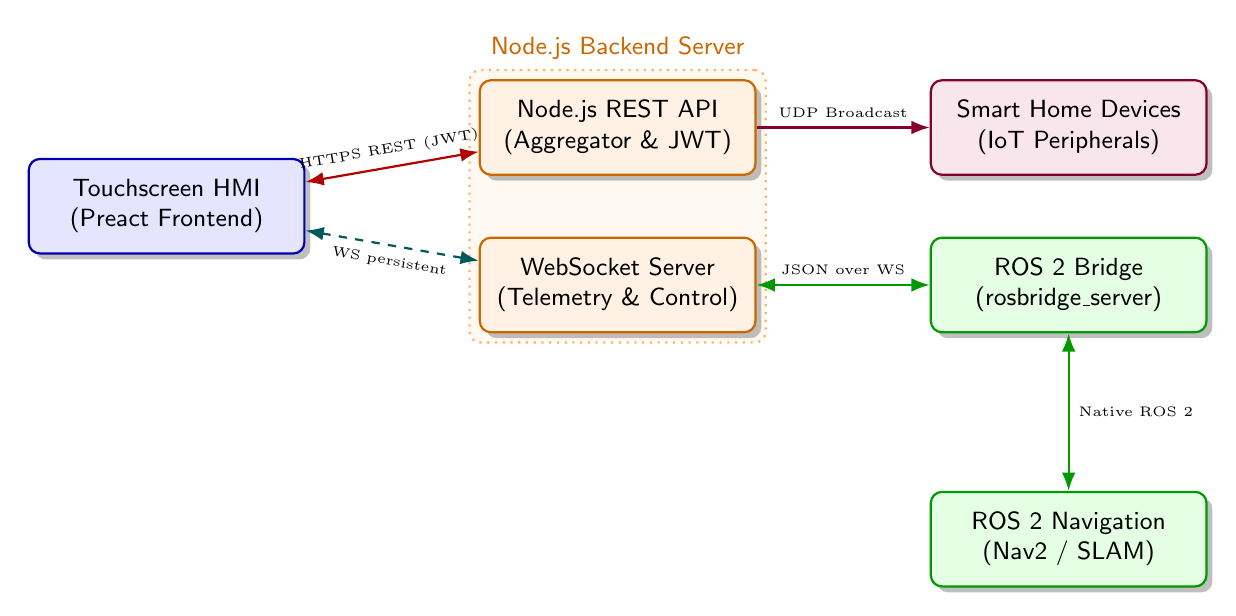
\begin{tikzpicture}[
    font=\sffamily\small,
    node distance=2.0cm and 2.2cm,
    clientNode/.style={rectangle, draw=blue!70!black, fill=blue!10, rounded corners, minimum width=3.5cm, minimum height=1.2cm, align=center, thick, drop shadow},
    serverNode/.style={rectangle, draw=orange!80!black, fill=orange!10, rounded corners, minimum width=3.5cm, minimum height=1.2cm, align=center, thick, drop shadow},
    hardwareNode/.style={rectangle, draw=green!60!black, fill=green!10, rounded corners, minimum width=3.5cm, minimum height=1.2cm, align=center, thick, drop shadow},
    peripheralNode/.style={rectangle, draw=purple!70!black, fill=purple!10, rounded corners, minimum width=3.5cm, minimum height=1.2cm, align=center, thick, drop shadow},
    httpArrow/.style={Latex-Latex, draw=red!70!black, thick},
    wsArrow/.style={Latex-Latex, draw=teal!70!black, dashed, thick},
    rosArrow/.style={Latex-Latex, draw=green!60!black, thick},
    udpArrow/.style={-Latex, draw=purple!70!black, thick}
]

    \node[clientNode] (hmi) {Touchscreen HMI\\(Preact Frontend)};
    
    \node[serverNode, right=of hmi, yshift=1cm] (express) {Node.js REST API\\(Aggregator \& JWT)};
    \node[serverNode, right=of hmi, yshift=-1cm] (wsServer) {WebSocket Server\\(Telemetry \& Control)};
    
    \node[hardwareNode, right=of wsServer] (rosbridge) {ROS 2 Bridge\\(rosbridge\_server)};
    \node[peripheralNode, right=of express] (iot) {Smart Home Devices\\(IoT Peripherals)};
    
    \node[hardwareNode, below=of rosbridge] (ros) {ROS 2 Navigation\\(Nav2 / SLAM)};

    \begin{scope}[on background layer]
        \node[draw=orange!60, fill=orange!5, dotted, thick, rounded corners, fit=(express) (wsServer), label={[orange!80!black]above:Node.js Backend Server}] (serverGroup) {};
    \end{scope}

    \draw[httpArrow] (hmi) -- node[above, sloped, font=\tiny] {HTTPS REST (JWT)} (express);
    \draw[wsArrow] (hmi) -- node[below, sloped, font=\tiny] {WS persistent} (wsServer);
    
    \draw[rosArrow] (wsServer) -- node[above, font=\tiny] {JSON over WS} (rosbridge);
    \draw[rosArrow] (rosbridge) -- node[right, font=\tiny] {Native ROS 2} (ros);
    \draw[udpArrow] (express) -- node[above, font=\tiny] {UDP Broadcast} (iot);

\end{tikzpicture}
\caption{Communication topology showing the dual transport paths (REST and WebSockets) between the Preact HMI, the Node.js server wrapper, and the robotic/IoT backends.}
\label{fig:hmi-server-comm-tikz}
\end{figure}

\subsection{Dual-Channel Transport Protocol}
The connection between the touchscreen client and the server leverages two distinct network protocols to optimize for different data transmission requirements:
\begin{itemize}
    \item \textbf{RESTful API Channel (Stateless HTTP/HTTPS)}: This channel is reserved for transactional, low-frequency control actions and query requests. Actions such as requesting a list of pre-configured rooms and coordinate goals, saving user network preferences, and invoking local network discovery scans for smart home devices are conducted via HTTP. To secure this channel, each request must include a signed JSON Web Token (JWT) in its authorization header. Payload verification is enforced on the server prior to controller execution, ensuring that only authenticated, properly formatted requests are processed.
    \item \textbf{WebSocket Channel (Persistent Duplex TCP)}: Real-time control and environmental updates require a low-latency, bidirectional data flow that cannot be efficiently sustained via request-response polling. A persistent WebSocket connection is established between the touchscreen and the server. This channel continuously transmits the wheelchair's telemetry state, occupancy grid update frames, robot position coordinates, and real-time linear/angular teleoperation velocity commands. By bypassing the overhead of standard HTTP handshakes and headers, this persistent socket minimizes latency, ensuring immediate responsiveness during gaze-control driving or manual navigation overrides.
\end{itemize}

\subsection{Serialization and Type Verification}
Data transmitted over both REST and WebSocket channels is structured using lightweight JavaScript Object Notation (JSON). In order to maintain system integrity, data contracts are defined on both ends. The client-side Preact application enforces structural validation using TypeScript types, while the server verifies incoming payloads against predefined schemas before routing them to the ROS 2 integration layer. This bidirectional verification ensures that malformed inputs, such as negative temperature bounds or out-of-range navigation coordinates, are intercepted and rejected at the application boundary, protecting the physical actuators from erratic signals.

\subsection{State Synchronization and Conflict Resolution}
The HMI client maintains local variables representing the status of connected devices (e.g. lighting states, active speed profiles, and active navigation goals). To keep the user interface consistent with the physical world, the system adopts an optimistic UI update model:
\begin{itemize}
    \item When a user changes a setting, such as turning off a smart light, the touchscreen UI immediately reflects the new state.
    \item The client issues an asynchronous HTTP command to the Node.js server.
    \item If the command fails (due to database lock or network disruption), the client captures the error, reverts the local state, and prompts the user with an error notification.
    \item System-critical parameters, including network configurations and current active themes, are persisted locally using the client browser's storage API, allowing the touchscreen HMI to re-initialize to its last known safe state immediately upon reboot.
\end{itemize}

\subsection{Connection Resiliency and Error Recovery}
Given that the touchscreen and the server communicate over local Wi-Fi or internal virtual networks, connection drops can occur. To prevent erratic behaviors, the system implements a robust connection lifecycle manager:
\begin{itemize}
    \item \textbf{Heartbeat Monitor}: The client and server exchange small keep-alive frames at regular intervals. If the client fails to receive a ping acknowledgement within $1500\text{ ms}$, the connection is flagged as degraded.
    \item \textbf{Safe Degradation}: Upon detecting a connection drop, the touchscreen interface automatically displays a prominent red warning banner and locks out manual drive commands, preventing the user from issuing steering requests while the state is uncertain.
    \item \textbf{Reconnection Strategy}: The client initiates a reconnection loop using exponential backoff.
    \item \textbf{Hardware Fail-Safe}: To ensure safety during teleoperation, the underlying ROS 2 velocity controller monitors the keep-alive signal. If no velocity update command is received from the HMI over the WebSocket channel within $500\text{ ms}$, the motor driver automatically halts the wheelchair, preventing runaway collisions in the event of an HMI crash or network failure.
\end{itemize}

\section{Home Dashboard}
The first view presented to the user is the Home Dashboard, implemented in \texttt{HomeView.tsx}. It serves as a visual launcher, providing a clean, distraction-free grid containing four high-contrast touch cards.

The primary functions displayed are:
\begin{itemize}
    \item \textbf{Map Navigation}: Navigates the user to the interactive map viewport for route visualization and destination selection.
    \item \textbf{Hands-Free Control}: Opens the radial eye-tracking interface, allowing users with severe paralysis to drive the chair or operate the home.
    \item \textbf{Smart Home}: Displays a dedicated grid for IoT smart appliance management.
    \item \textbf{System Settings}: Grants access to theme adjustments, notifications, and bridge endpoints.
\end{itemize}

The layout uses a two-column, two-row responsive grid with rounded panels (\texttt{rounded-2xl}), subtle gradients, and prominent SVG icons. The design is optimized for low visual clutter to ensure readability under varying light conditions.

\begin{figure}[H]
\centering
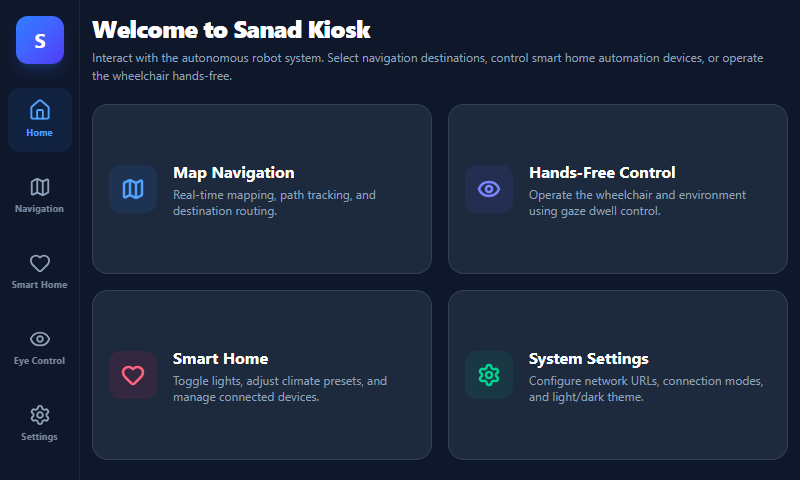
\includegraphics[width=0.6\textwidth]{figures/ch07/home_dark.png}
\caption{Home Dashboard UI in Dark Mode showing the high-contrast button grid.}
\label{fig:home-dark}
\end{figure}

\section{Real-Time Map \& Navigation Interface}
The map interface (\texttt{MapView.tsx}) is the most complex module in the touchscreen package. It integrates a 2D rendering pipeline to present an occupancy grid map constructed by the SLAM (Simultaneous Localization and Mapping) perception stack.

\subsection{Occupancy Grid Model}
The map data is received as a ROS message containing the map metadata and cell weights:
\begin{equation}
M = \{H, I, D\}
\end{equation}
where $H$ is the header containing coordinate frame references and stamps, $I$ is the map metadata (resolution, grid width, grid height, and origin pose), and $D$ is a one-dimensional array of occupancy probability values:
\begin{equation}
d_i \in [-1, 0, \dots, 100]
\end{equation}
where $-1$ represents an unexplored cell, $0$ is free space, and $100$ is a confirmed obstacle.

\subsection{Map Rendering Canvas}
In \texttt{MapCanvas.tsx}, the occupancy grid data is read and parsed. A canvas rendering pipeline translates the 1D array into an image bitmap using offscreen canvas buffers. The resolution of the map (typically $0.05$ meters/pixel) is used to draw the boundary walls, corridors, and obstacle points.
A custom coordinate transformation handles mapping between the ROS world coordinate frame (origin at center of SLAM mapping) and the local HTML5 canvas coordinate frame (origin at top-left, measured in pixels):
\begin{align}
x_{\text{canvas}} &= \frac{x_{\text{world}} - x_{\text{origin}}}{\text{resolution}} \\
y_{\text{canvas}} &= \text{height}_{\text{grid}} - \frac{y_{\text{world}} - y_{\text{origin}}}{\text{resolution}}
\end{align}

\subsection{Robot Pose \& Navigation Control}
The robot's current position and heading ($x, y, \theta$) are retrieved from the coordinate transform tree (\texttt{/tf}) and rendered as a custom oriented triangle icon on top of the map. 
The user can navigate the wheelchair in two ways:
\begin{itemize}
    \item \textbf{Tap-to-Goal}: Clicking anywhere on the map canvas triggers a callback that translates the canvas pixel coordinates back to a ROS pose. This coordinates are sent to the Nav2 Action Server as a new navigation goal.
    \item \textbf{Quick Navigation Sidebar}: A drawer list displaying saved destinations (e.g., "Bedroom", "Kitchen", "Living Room"). Tapping a destination sends the pre-registered coordinates of that room.
\end{itemize}

During navigation, a dedicated status card displays feedback retrieved from the Action Server, including the remaining distance in meters, the estimated time remaining in seconds (ETA), and recovery behaviors triggered. A cancel button is available to halt autonomous motion immediately.

\begin{figure}[H]
\centering
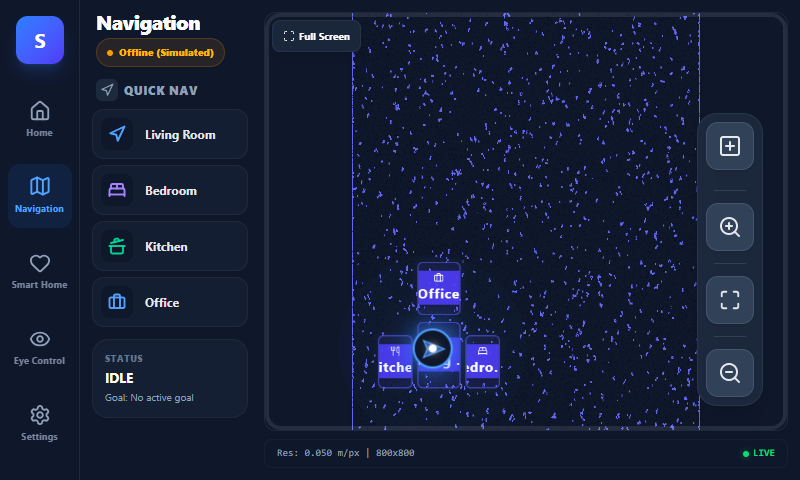
\includegraphics[width=0.9\textwidth]{figures/ch07/map_overview.png}
\caption{Map Viewport showing the 2D occupancy grid, registered rooms, and the Quick Navigation sidebar panel.}
\label{fig:map-overview}
\end{figure}

\section{Smart Home Control Panel}
The smart home integration interface (\texttt{SmartHomeView.tsx}) allows users to control IoT appliances in their home directly from the wheelchair touchscreen. It communicates with the intermediate Node.js server to monitor and control devices.

\subsection{Device Discovery}
By tapping the "Scan Network" button, the HMI triggers a network-wide discovery protocol. The server sends a UDP broadcast command on the local subnet to detect active smart appliances. Discovered devices are returned as an array, including their unique hardware ID, name, IP address, control type, and current state.

\subsection{Device Organization \& Control Widgets}
The application automatically categorizes discovered devices based on name and category metadata, grouping them into five clear visual sections: Lighting, Climate, Security, Media, and Other.
Each device category maps to a specialized control widget, as defined in Table \ref{tab:smart-home-controls}.

\begin{table}[H]
\centering
\caption{Smart Home Device Control Widgets}
\label{tab:smart-home-controls}
\begin{tabularx}{\textwidth}{|l|l|>{\raggedright\arraybackslash}X|l|}
\hline
\textbf{Device Type} & \textbf{Control Type} & \textbf{UI Widget Used} & \textbf{Example Commands} \\ \hline
Smart Light & \texttt{toggle} & Sliding toggle switch & \texttt{turn\_on} / \texttt{turn\_off} \\ \hline
Air Conditioner & \texttt{slider} & Horizontal range input slider (0--30) & \texttt{set\_temperature} (Celsius) \\ \hline
Media / TV & \texttt{toggle} & Sliding toggle switch & \texttt{power\_on} / \texttt{power\_off} \\ \hline
Door Lock & \texttt{button} & Instant click action button & \texttt{lock} / \texttt{unlock} \\ \hline
Dimmer Switch & \texttt{slider} & Horizontal range input slider (0--100) & \texttt{set\_brightness} \\ \hline
\end{tabularx}
\end{table}

\begin{figure}[H]
\centering
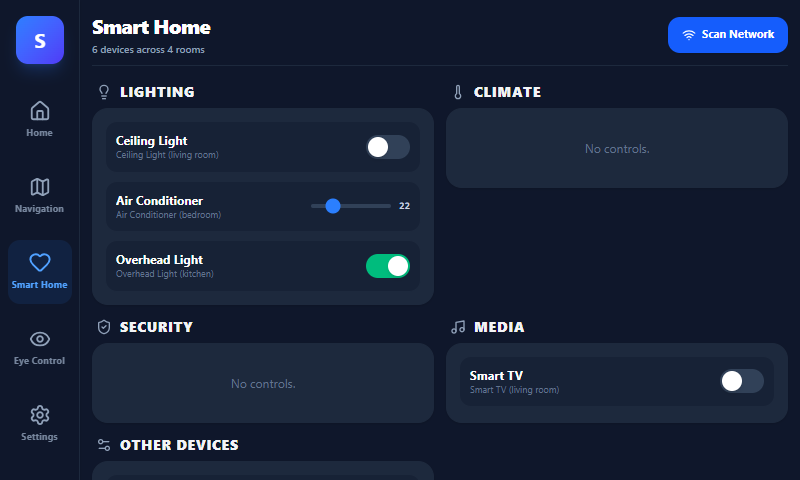
\includegraphics[width=0.9\textwidth]{figures/ch07/smarthome_panel.png}
\caption{Smart Home control panel showing active device controls grouped into Lighting, Climate, and Media sections.}
\label{fig:smarthome-panel}
\end{figure}

\section{Eye Tracking Interface \& Gaze Dwell}
For users with quadriplegia or advanced neuromuscular disorders (such as Amyotrophic Lateral Sclerosis or Multiple Sclerosis), standard physical touch control is not possible. For these users, the touchscreen serves as the primary visual display for an \textbf{Eye Tracking Interface} (\texttt{EyeControlView.tsx}). The hardware details of the physical infrared gaze cameras are discussed in later chapters; this section focuses on the software implementation of the radial gaze-wheel layout and the dwell-selection algorithm.

\subsection{Gaze Wheel Menu System}
The gaze interface is built as a radial menu (\texttt{GazeWheel.tsx}). Traditional grids are difficult for eye tracking because the gaze points can drift, leading to accidental selection of adjacent cells. A circular menu divides the screen into large pie-slice sectors around a central neutral region. This layout maximizes the distance between selectable areas, improving reliability.

The radial menu is hierarchical:
\begin{itemize}
    \item \textbf{Main Menu}: Displays top-level categories, including Navigation, Toggle Lights, Thermostat, Media, Door Locks, Wheelchair Drive, and Dwell Settings.
    \item \textbf{Sub-Menu - Navigation}: Dynamically lists registered rooms (e.g. Living Room, Bedroom) derived from \texttt{useRooms.ts}.
    \item \textbf{Sub-Menu - Wheelchair}: Displays motor commands: Forward, Turn Left, Stop, Turn Right, and Backward.
    \item \textbf{Sub-Menu - Dwell Settings}: Allows adjusting the validation timer to match the user's calibration quality.
\end{itemize}

\subsection{Gaze Dwell Selection Algorithm}
To register a select action without a physical click, the software uses a \textbf{gaze dwell mechanism} (\texttt{useGazeDwell.ts}). When the eye tracker detects the user's focus on a specific sector, a validation timer begins.
Let $S_i$ be the targeted sector, and $t_{\text{hover}}$ be the continuous duration the gaze remains within the sector boundary. The progress fraction $P(S_i)$ is computed at $30\text{ ms}$ intervals:
\begin{equation}
P(S_i) = \min\left(1, \frac{t_{\text{hover}}}{T_{\text{dwell}}}\right)
\end{equation}
where $T_{\text{dwell}}$ is the configurable dwell time selected by the user. 
Visually, this progress is rendered as a circular progress ring drawing around the sector. If $P(S_i) \geq 1.0$, the selection is confirmed, the action callback is fired, and the interface triggers a brief visual flash.
To prevent accidental repeated activations (the "Midas touch" problem), a cooldown state is immediately entered:
\begin{equation}
t_{\text{cooldown}} = 600\text{ ms}
\end{equation}
During this period, all selections are locked out. If the user's gaze drifts out of the sector at any point before $P(S_i) = 1.0$, the timer is cleared and the progress resets to $0$. 

\begin{figure}[H]
\centering
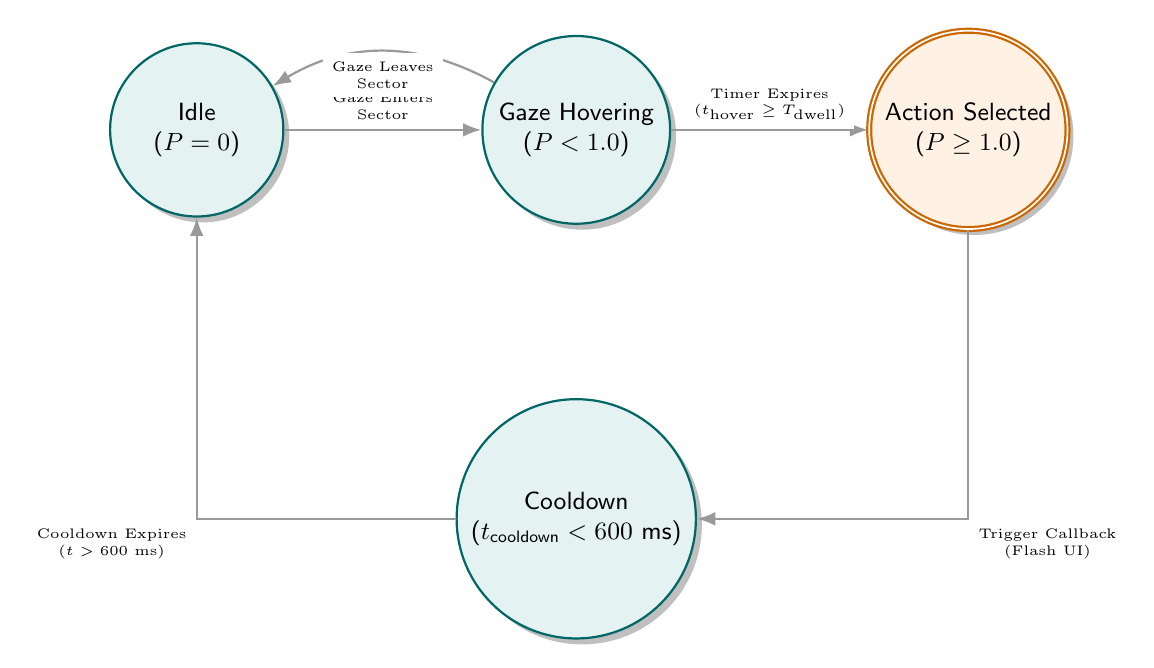
\begin{tikzpicture}[
    font=\sffamily\small,
    node distance=2.2cm and 2.5cm,
    state/.style={circle, draw=teal!80!black, fill=teal!10, thick, minimum size=2.2cm, align=center, drop shadow},
    triggerState/.style={circle, draw=orange!80!black, fill=orange!10, thick, minimum size=2.2cm, align=center, double, drop shadow},
    arrow/.style={-Latex, thick, draw=gray!80},
    transLabel/.style={font=\tiny, fill=white, align=center}
]

    % States
    \node[state] (idle) {Idle\\($P = 0$)};
    \node[state, right=of idle] (hover) {Gaze Hovering\\($P < 1.0$)};
    \node[triggerState, right=of hover] (selected) {Action Selected\\($P \ge 1.0$)};
    \node[state, below=of hover] (cooldown) {Cooldown\\($t_{\text{cooldown}} < 600\text{ ms}$)};

    % Transitions
    \draw[arrow] (idle) -- node[above, transLabel] {Gaze Enters\\Sector} (hover);
    \draw[arrow] (hover) -- node[above, transLabel] {Timer Expires\\($t_{\text{hover}} \ge T_{\text{dwell}}$)} (selected);
    
    % Hover to Idle (Reset)
    \draw[arrow, bend right=30] (hover) to node[below, transLabel] {Gaze Leaves\\Sector} (idle);
    
    % Selected to Cooldown
    \draw[arrow] (selected) |- node[below right, transLabel] {Trigger Callback\\(Flash UI)} (cooldown);
    
    % Cooldown to Idle
    \draw[arrow] (cooldown) -| node[below left, transLabel] {Cooldown Expires\\($t > 600\text{ ms}$)} (idle);

\end{tikzpicture}
\caption{State machine diagram illustrating the gaze-dwell selection and error-prevention lifecycle.}
\label{fig:gaze-dwell-state-machine}
\end{figure}

\begin{figure}[H]
\centering
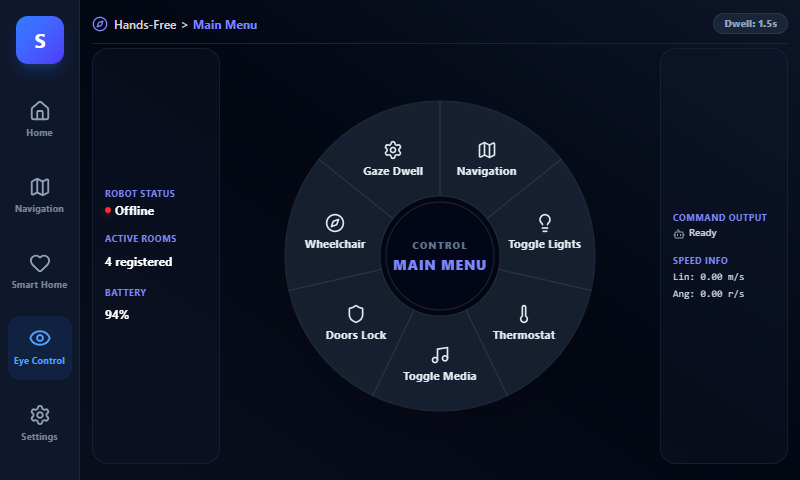
\includegraphics[width=0.7\textwidth]{figures/ch07/gaze_wheel_main.png}
\caption{Main Menu of the hands-free gaze interface, showing the radial layout and central "neutral" sector.}
\label{fig:gaze-wheel-main}
\end{figure}

\section{Wheelchair Teleoperation Interface}
For users operating the wheelchair through alternative controllers or direct screen interaction, a software \textbf{Wheelchair Teleoperation Mode} is integrated. In this mode, the client sends velocity commands directly to the robot.

The wheelchair's target velocity command is defined by the linear velocity $v$ and angular velocity $\omega$:
\begin{align}
v &\in [-1.0, 1.0]\text{ m/s} \quad \text{(normalized)} \\
\omega &\in [-1.0, 1.0]\text{ rad/s} \quad \text{(normalized)}
\end{align}
These inputs are sent via the \texttt{updateVelocity(linear, angular)} function in \texttt{IWheelchairService}.
When using the eye-control drive sub-wheel, the directional commands map to pre-configured safe velocity thresholds:
\begin{itemize}
    \item \textbf{Move Forward}: $v = 0.3\text{ m/s}, \omega = 0.0\text{ rad/s}$
    \item \textbf{Turn Left}: $v = 0.0\text{ m/s}, \omega = 0.4\text{ rad/s}$
    \item \textbf{Turn Right}: $v = 0.0\text{ m/s}, \omega = -0.4\text{ rad/s}$
    \item \textbf{Move Backward}: $v = -0.3\text{ m/s}, \omega = 0.0\text{ rad/s}$
    \item \textbf{STOP}: $v = 0.0\text{ m/s}, \omega = 0.0\text{ rad/s}$
\end{itemize}



Safety is a primary design consideration. In addition to the physical emergency stop switches, a software safety stop is always visible as a red octagon in the center of the driving sub-wheel. Additionally, the wheelchair controller automatically times out and halts the motors if it does not receive a keep-alive velocity command within $500\text{ ms}$.

\section{Settings \& Configuration Management}
The settings view (\texttt{SettingsView.tsx}) manages user preferences and interface parameters.
It is divided into three sections:
\begin{itemize}
    \item \textbf{Appearance}: Allows selecting the display theme (Light, Dark, or System Sync).
    \item \textbf{Connection}: Configures the backend integration mode (NATIVE, SERVER, or SIMULATION) and allows overriding WebSocket/REST API URLs to adapt to local networks.
    \item \textbf{Notifications}: Toggles desktop and audio alerts for obstacle warnings and connection losses.
\end{itemize}

All configuration parameters are stored locally on the client device using the browser's \texttt{localStorage} API. This ensures settings persist across system reboots. To ensure clean state initialization, saving new connection parameters resets the health flag and refreshes the browser window using \texttt{window.location.reload()}, which re-initializes all factories and initiates clean WebSocket connections to the new endpoints.

\begin{figure}[H]
\centering
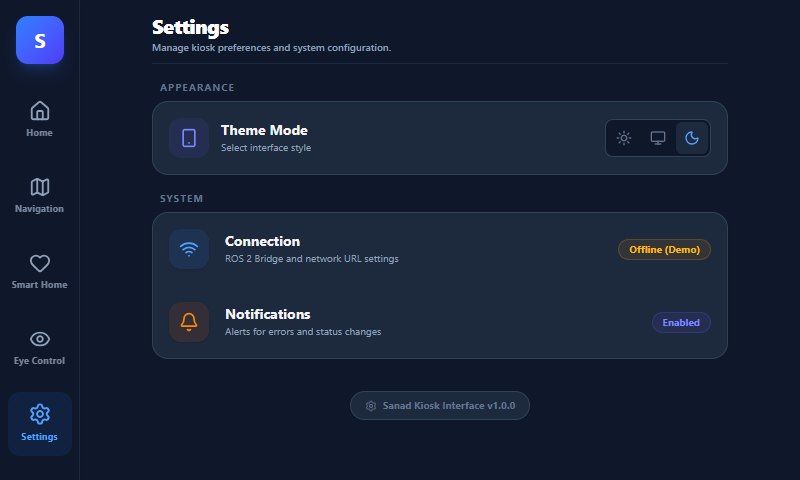
\includegraphics[width=0.7\textwidth]{figures/ch07/settings_overview.png}
\caption{Settings view showing configuration options for themes, network endpoints, and system parameters.}
\label{fig:settings-overview}
\end{figure}

\section{Accessibility Design}
Providing full access to users with motor impairments requires strict adherence to web accessibility guidelines (WCAG 2.1 Level AA).

\subsection{ARIA Attributes \& Semantics}
The interface uses semantic HTML structure and ARIA (Accessible Rich Internet Applications) attributes to support screen readers and switch-access devices. 
Table \ref{tab:accessibility-aria} lists the ARIA patterns used in the interface.

\begin{table}[H]
\centering
\caption{Application ARIA Accessibility Patterns}
\label{tab:accessibility-aria}
\begin{tabularx}{\textwidth}{|l|>{\raggedright\arraybackslash}X|>{\raggedright\arraybackslash}X|>{\raggedright\arraybackslash}X|}
\hline
\textbf{Pattern} & \textbf{ARIA Attributes} & \textbf{Target Element} & \textbf{Usage Rationale} \\ \hline
Tab Control & \texttt{role="tablist"}, \texttt{role="tab"} & Sidebar navigation buttons & Represents the primary application sections. \\ \hline
Tab Panel & \texttt{role="tabpanel"} & Core viewport frames & Links each panel container to its corresponding tab button. \\ \hline
Selection State & \texttt{aria-selected="true"} & Active tab element & Identifies the currently selected view. \\ \hline
Control State & \texttt{aria-checked="true"} & Selected radio button & Indicates the active option (e.g. active theme). \\ \hline
Grid Lists & \texttt{role="list"}, \texttt{role="listitem"} & Home menu dashboard buttons & Groups launch shortcuts into structured groups. \\ \hline
Labels & \texttt{aria-label="string"} & Custom icon-only buttons & Provides clear descriptions for controls without text labels. \\ \hline
\end{tabularx}
\end{table}

\subsection{Keyboard \& Arrow Key Navigation Hook}
To accommodate mechanical switches (such as sip-and-puff controls or head-rest switches) that mimic standard keyboard events, a custom navigation hook was developed (\texttt{useArrowNavigation.ts}).
This hook captures keyboard focus events within containers (like \texttt{role="tablist"} or \texttt{role="list"} grids). When an arrow key is pressed, the hook intercepts the default browser event, computes the target element's index, and moves focus programmatically. This allows full control over the application's tabs, buttons, sliders, and modal dialogs using only four keyboard events (or a single scanning switch). Focus indicators are styled with highly visible borders (\texttt{focus-visible:ring-4}) to assist users with visual impairments.

\section{Dark Mode \& Theming System}
To ensure the interface is readable in different environments (such as direct sunlight or dark rooms), the application features a persistent theming system (\texttt{useTheme.ts}). 

The theme can be set to:
\begin{itemize}
    \item \textbf{Light Mode}: Optimizes contrast for bright outdoor environments, using slate-colored text against a pure white background.
    \item \textbf{Dark Mode}: Reduces glare and eye strain in dim indoor settings, using white text against a deep slate background.
    \item \textbf{System Mode}: Syncs the app theme with the operating system's setting using a CSS media query.
\end{itemize}

The theme is applied by adding the \texttt{"dark"} class to the root HTML element, enabling Tailwind's \texttt{dark:} styling variants for all components. Transitions are smoothed with CSS rules (\texttt{transition-colors duration-300}) to prevent jarring flashes when changing themes.



\section{Performance Metrics \& Optimization}
The interface must perform reliably on low-cost, low-power single-board computers (SBCs). To verify this, Lighthouse audits and performance benchmarks were run on target hardware. Table \ref{tab:perf-metrics} lists the measured performance parameters.

\begin{table}[H]
\centering
\caption{Measured HMI Performance and Size Metrics}
\label{tab:perf-metrics}
\begin{tabularx}{\textwidth}{|>{\raggedright\arraybackslash}X|c|c|>{\raggedright\arraybackslash}X|}
\hline
\textbf{Performance Metric} & \textbf{Target Limit} & \textbf{Measured Value} & \textbf{Measurement Tool} \\ \hline
First Contentful Paint (FCP) & < 1.5 s & 0.65 s & Lighthouse Audit \\ \hline
Largest Contentful Paint (LCP) & < 2.5 s & 0.98 s & Lighthouse Audit \\ \hline
Total Blocking Time (TBT) & < 200 ms & 45 ms & Lighthouse Audit \\ \hline
Cumulative Layout Shift (CLS) & < 0.1 & 0.01 & Lighthouse Audit \\ \hline
Production Bundle Size (Compressed) & < 250 KB & 112 KB & Vite Production Build \\ \hline
Map Canvas Frame Rate & > 30 fps & 58 fps & Chrome Performance Monitor \\ \hline
Gaze-Dwell Trigger Latency & < 50 ms & 4 ms & Chrome Performance Monitor \\ \hline
Accessibility Audit Score & > 95 & 100 / 100 & Lighthouse Accessibility \\ \hline
\end{tabularx}
\end{table}

These performance targets are met through several optimizations:
\begin{itemize}
    \item \textbf{Preact VDOM diffing}: Minimizes memory allocation and DOM manipulations, resulting in low TBT.
    \item \textbf{DOM Node Reuse}: The tab rendering system hides unused views using CSS classes, avoiding the performance cost of repeatedly mounting and unmounting the map canvas.
    \item \textbf{Canvas Rendering}: Drawing the occupancy grid directly to an HTML5 canvas bypasses the DOM engine entirely, allowing smooth map rendering and pan/zoom performance.
    \item \textbf{Singleton Factories}: Limits connection overhead by sharing WebSocket and API client instances across all views.
\end{itemize}

\section{Summary and Transition}
This chapter has described the development of the lightweight Preact on-board touchscreen interface, detailing its integration and accessibility modalities. The next chapter, Chapter 8 (Eye Tracking), presents the computer-vision eye-tracking subsystem that maps pupil movements to coordinates for hands-free menu selection on this display.


\chapterseparator{Chapter 8}
\setcounter{chapter}{8} 
\chapter*{Chapter (8): Eye Tracking}
\addcontentsline{toc}{chapter}{Chapter (8): Eye Tracking} 
\setcounter{section}{0}

\section{Chapter Preview}
\label{sec:eye_tracking}
This chapter details the design of the webcam-based eye-tracking module developed for non-verbal or locked-in Sanad users. It outlines the camera hardware, MediaPipe face and iris landmark detection algorithms, the head-pose independent gaze vector calculation, calibration techniques, command mapping schemes, and performance evaluations.

% ----------------------------------------------------------------
\section{Camera Hardware}
% ----------------------------------------------------------------

The camera we used is EMEET C955. It works with 1920 x 1080 resolution and is connected via USB. It is mounted at the top-centre of the touchscreen bezel, angled
5--10° upward toward the user at a working distance of 35--45~cm. Frames are captured
in BGR at 30~fps and are \textbf{horizontally mirrored} immediately on read, so cursor
motion matches the user's natural gaze direction.

\begin{figure}[H]
\centering
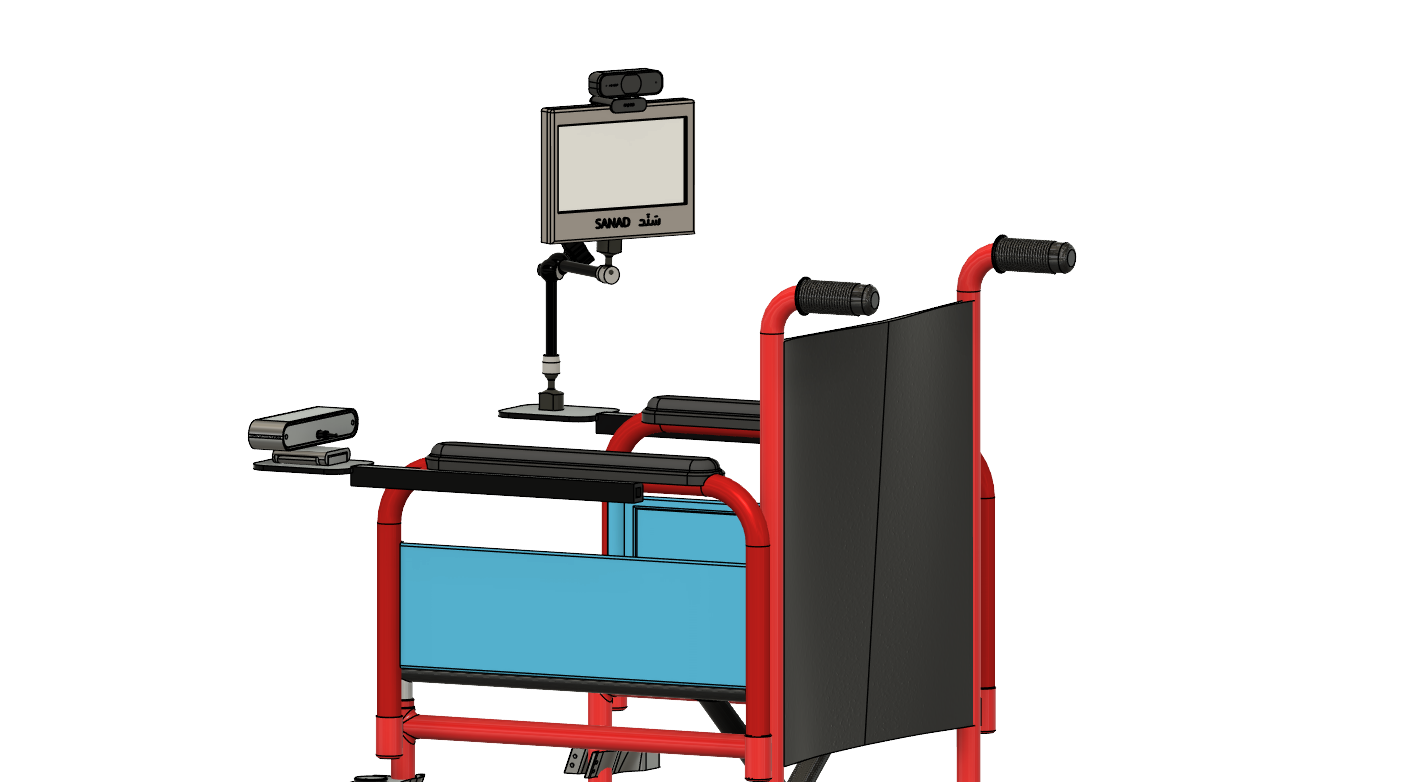
\includegraphics[width=500]{figures/ch08/20}
\label{fig:camera_hardware}
\end{figure}

\newpage

% ----------------------------------------------------------------
\subsection{Eye Tracking Algorithm: MediaPipe FaceLandmarker}
% ----------------------------------------------------------------
\subsubsection{Algorithm Selection}

Several approaches were evaluated against two criteria: real-time CPU-only performance on
the Pi~4 and accuracy sufficient for command-zone discrimination.

\begin{table}[H]
\centering
\caption{Eye Tracking Approach Comparison}
\label{tab:et_algorithm_comparison}
\begin{tabular}{p{3.5cm}p{2.0cm}p{2.5cm}p{2.0cm}p{4.0cm}}
\toprule
\textbf{Approach} & \textbf{CPU (Pi~4)} & \textbf{Accuracy} & \textbf{Decision} & \textbf{Reason} \\
\midrule
Tobii Eye Tracker 5
  & N/A (USB)   & Very High
  & Rejected & Cost ($>$\$200); proprietary SDK \\[3pt]
iTracker CNN
  & $>$90\%     & High
  & Rejected & Exceeds Pi~4 CPU budget \\[3pt]
OpenFace + dlib
  & 70--80\%    & Moderate--High
  & Rejected & Marginal remaining headroom \\[3pt]
GazeTracking (pupil)
  & 20--30\%    & Low--Moderate
  & Rejected & No iris model; poor low-light \\[3pt]
\textbf{MediaPipe FaceLandmarker}
  & \textbf{30--45\%} & \textbf{Moderate--High}
  & \textbf{Selected} & \textbf{Reasonable accuracy with suitable computational load} \\
\bottomrule
\end{tabular}
\end{table}

\textbf{MediaPipe FaceLandmarker} (Tasks API, \texttt{mediapipe} $\geq$ 0.10) was selected
as the optimal trade-off between accuracy and embedded performance. It ships a
float16-quantised TFLite model (\texttt{face\_landmarker.task}, $\approx$3.6~MB) that
produces \textbf{478 facial landmarks} — including a dedicated iris sub-model — at 20--28~fps
on the Pi~4 CPU without GPU. The model runs in \textbf{VIDEO mode}, feeding each frame with
a monotonically increasing timestamp so the tracker exploits temporal context across frames
for improved stability.

\begin{figure}[H]
\centering
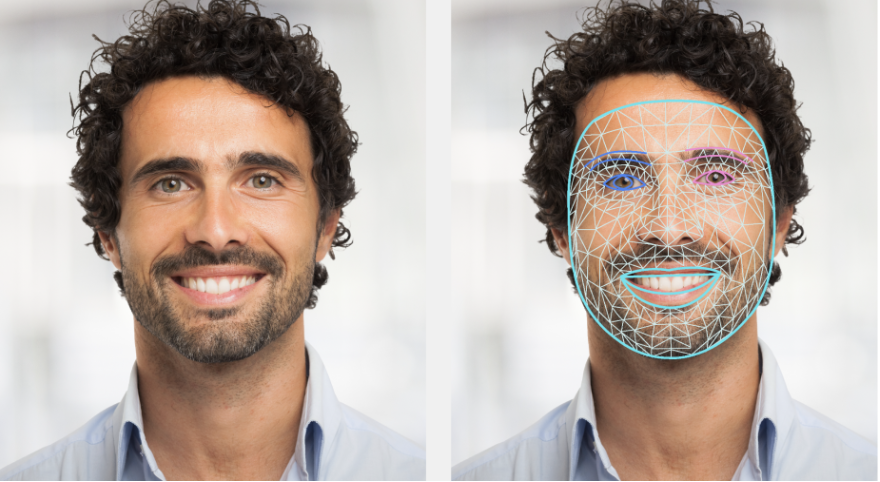
\includegraphics[width=300]{figures/ch08/fig2_latex.png}
\label{fig:mediapipe_face_landmark}
\end{figure}

\subsection{Iris Landmark Indices}

The iris centre is computed as the centroid of four
boundary landmarks per eye (indices 469–472 for the left eye, 474–477 for
the right). Its position is expressed as a fraction of the eye's own width
using the inner and outer eye corners (indices 33/133 and 362/263) as the
reference frame, making the measurement inherently robust to small head
translations.

\begin{table}[h!]
\centering
\caption{MediaPipe Landmark Indices Used by the Eye Tracking Pipeline}
\label{tab:et_landmarks}
\begin{tabular}{lll}
\toprule
\textbf{Landmark Group} & \textbf{Indices} & \textbf{Usage} \\
\midrule
Left iris boundary      & 469, 470, 471, 472      & Gaze X/Y (user's right eye) \\
Right iris boundary     & 474, 475, 476, 477      & Gaze X/Y (user's left eye) \\
Left eye corners        & 33 (inner), 133 (outer) & Horizontal normalisation \\
Right eye corners       & 362 (inner), 263 (outer) & Horizontal normalisation \\
Left eyelid top/bottom  & 159 / 145               & EAR blink detection \\
Right eyelid top/bottom & 386 / 374               & EAR blink detection \\
\bottomrule
\end{tabular}
\end{table}

\begin{figure}[H]
\centering
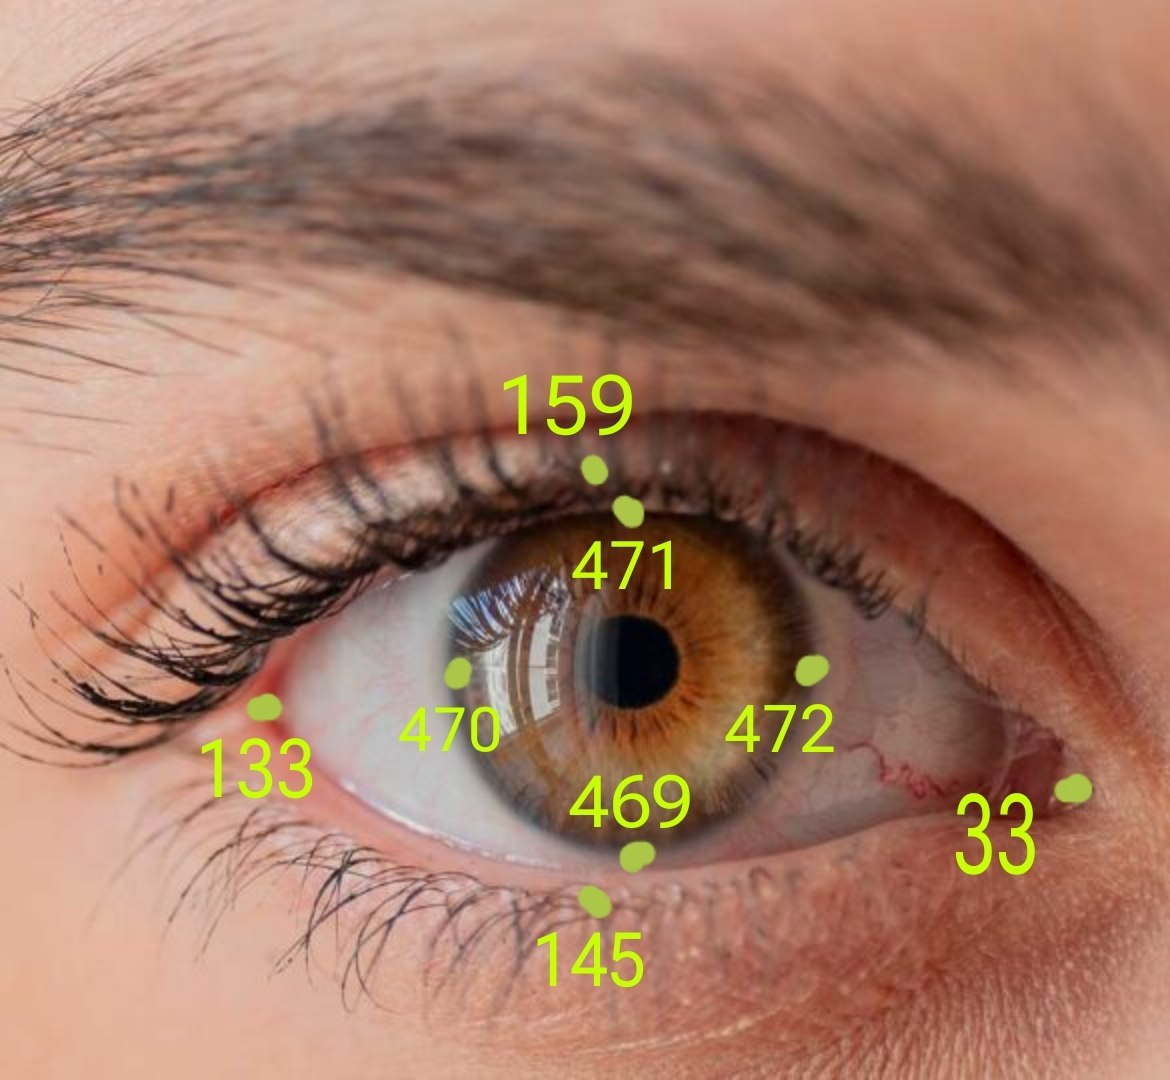
\includegraphics[width=300]{figures/ch08/fig3_latex}
\label{fig:iris_indicies}
\end{figure}

% ----------------------------------------------------------------
\section{Gaze Vector Computation: Iris Ratio Method}
% ----------------------------------------------------------------

The gaze position is computed using the \textbf{Iris Ratio Method}, which expresses the
iris location as a fraction of the eye's own extent. This makes the measurement inherently
insensitive to small head translations.

\textbf{Step 1 — Iris centre:} The four boundary landmarks per eye are averaged to pixel
coordinates $(x_c, y_c)$. Both eyes are averaged to reduce single-eye occlusion noise.

\begin{equation}
    x_c = \frac{1}{4} \sum_{k \in \mathcal{I}} \lambda_k^x \cdot W, \qquad
    y_c = \frac{1}{4} \sum_{k \in \mathcal{I}} \lambda_k^y \cdot H
    \label{eq:iris_centre}
\end{equation}

\textbf{Step 2 — Iris ratio:} The iris displacement within the eye socket is expressed as a
normalised ratio, where $x_L, x_R$ are the eye corner $x$-coordinates, $y_M$ is the
vertical eye midline, and $w_e = x_R - x_L$ is the eye width:

\begin{align}
    r_h &= \frac{x_c - x_L}{w_e} - 0.5, \qquad
    r_v  = \frac{y_c - y_M}{w_e}
    \label{eq:ratios}
\end{align}

\textbf{Step 3 — Normalisation:} Per-user offset ($\delta$) and range ($\rho$) calibration
parameters are applied:
$\hat{r} = (r - \delta) / \rho$.

\textbf{Step 4 — Non-linear power curve:} A signed power-law sharpens central precision
while preserving full edge access:

\begin{equation}
    \tilde{r} = \operatorname{sign}(\hat{r}) \cdot |\hat{r}|^{1.2}
    \label{eq:power_curve}
\end{equation}

\textbf{Step 5 — Screen mapping:} The result is clamped and remapped to $[0, 1]$: \newline
$g = \bigl(\operatorname{clip}(\tilde{r}, -1, 1) + 1\bigr) / 2$.
The final pair $(g_x, g_y)$ is published on \newline \texttt{/eye\_tracking/gaze\_position} at 30~Hz.

% ----------------------------------------------------------------
\section{Blink Detection and Temporal Filtering}
% ----------------------------------------------------------------

\textbf{Eye Aspect Ratio (EAR):} Blink and eye-closure events are detected using the
EAR metric, defined as the ratio of vertical eye opening to horizontal
eye span. Open eyes yield EAR $\approx 0.28$--$0.35$; a closed eye drops below the
threshold $\theta_{\text{EAR}} = 0.20$.

\begin{equation}
    \text{EAR} = \frac{\| \mathbf{p}_{\text{top}} - \mathbf{p}_{\text{bottom}} \|}
                      {\| \mathbf{p}_{\text{left}} - \mathbf{p}_{\text{right}} \|}
    \label{eq:ear}
\end{equation}

The eye state published on \texttt{/eye\_tracking/eye\_state} is \texttt{"open"} when
$\text{EAR} \geq \theta$, \texttt{"blink"} on the first frame of closure, and
\texttt{"closed"} on sustained closure.

\textbf{EMA smoothing:} Raw iris positions are smoothed by an Exponential Moving Average
applied only during open-eye frames to suppress micro-saccade jitter:

\begin{equation}
    \hat{g}_t = \alpha \cdot g_t + (1 - \alpha)\cdot\hat{g}_{t-1}, \qquad \alpha = 0.30
    \label{eq:ema}
\end{equation}

On blink or closure, the EMA update freezes and the last valid position is held.

\textbf{Blink-rewind buffer:} During a natural blink the upper eyelid physically pushes
the iris downward before closure, which would otherwise shift the cursor toward the screen
bottom on every blink. A \textbf{circular history buffer}
(\texttt{deque(maxlen=7)}, $\approx$230~ms) stores recent open-eye gaze positions.
On blink detection, the cursor is rewound to the oldest buffer entry — the pre-blink gaze
state — making blinks completely transparent to cursor position.

% ----------------------------------------------------------------
\section{Calibration}
% ----------------------------------------------------------------

Calibration is performed by adjusting per-user parameters in \newline
\texttt{config/eye\_tracking\_params.yaml}. With the debug overlay enabled, the user
looks at screen centre to set offsets, then at the edges to set range; the full procedure
takes under two minutes and the profile is saved for reuse.

\begin{table}[H]
\centering
\caption{Eye Tracking Key Configuration Parameters}
\label{tab:et_calib_params}
\begin{tabular}{lll}
\toprule
\textbf{Parameter} & \textbf{Default} & \textbf{Description} \\
\midrule
\texttt{gaze\_range\_horizontal} & 0.040   & Max horizontal iris displacement \\
\texttt{gaze\_range\_vertical}   & 0.020   & Max vertical iris displacement \\
\texttt{gaze\_offset\_horizontal}& 0.000   & Resting-gaze horizontal zero-point \\
\texttt{gaze\_offset\_vertical}  & $-$0.015 & Resting-gaze vertical zero-point \\
\texttt{gaze\_smoothing}         & 0.30    & EMA factor $\alpha$ (lower = smoother, laggier) \\
\texttt{ear\_threshold}          & 0.20    & EAR closure threshold \\
\texttt{click\_hold\_time}       & 2.0\,s  & Sustained closure duration to emit a click \\
\texttt{command\_cooldown}       & 1.0\,s  & Minimum interval between commands \\
\bottomrule
\end{tabular}
\end{table}

% ----------------------------------------------------------------
\section{Gaze-to-Command Mapping: Design Iterations}
% ----------------------------------------------------------------

Translating raw gaze data into wheelchair commands is the most user-facing design challenge
in the eye tracking module. Because Sanad targets users with severe or total loss of motor
function, every candidate mechanism must work with \textit{zero} reliance on hands, fingers,
or deliberate physical movement. The team evaluated four distinct interaction paradigms in
sequence, each informing the next, before arriving at the final design. The following
subsections document each iteration — its rationale, prototype, observed failure modes, and
the reasons it was either rejected or carried forward.

% ......................................
\subsection{Iteration 1 — Hand Gesture Control (Rejected)}
% ......................................

The first candidate explored was \textbf{hand gesture recognition} using the camera feed.
Gestures such as a raised palm, pointing finger, or directional swipe would be mapped to
navigation commands. This approach is computationally mature and widely used in consumer
devices.

However, it was rejected immediately after reviewing the primary user profile. ALS patients
— the core target population — lose voluntary muscle control progressively, with upper-limb
paralysis typically preceding or concurrent with the need for a powered wheelchair.
Requiring any deliberate hand or arm movement directly contradicts the accessibility
objective of the module. No prototype was built for this iteration.

% ......................................
\subsection{Iteration 2 — Blink-Coded Commands (Rejected)}
% ......................................

The second design attempted to repurpose natural eye closure as a \textbf{morse-code-like
input channel}. Different blink sequences were mapped to different commands: for example,
two rapid blinks triggered a \textit{right} movement, three rapid blinks triggered
\textit{left}, a sustained 3-second eye closure confirmed a selection, and other patterns
encoded \textit{forward}, \textit{backward}, and \textit{back/cancel}. The appeal of this
system was that it required only the eyes — no gaze tracking hardware beyond a webcam — and
could in principle provide a rich enough vocabulary to cover all necessary commands.

A prototype was built and tested. The following failure modes were observed:

\begin{itemize}
    \item \textbf{High false-positive rate:} A healthy person blinks involuntarily 15--20
    times per minute. Every natural blink was a potential accidental command. The system
    struggled fundamentally to distinguish an intentional ``two-blink right'' sequence from
    a natural blink followed by a second natural blink a fraction of a second later. Tuning
    the inter-blink timing threshold was a losing battle: tightening it caused missed
    intentional commands; loosening it caused more false triggers.

    \item \textbf{Severe eye fatigue:} Performing deliberate, counted blink sequences
    continuously throughout a navigation session required constant conscious effort from the
    user. Testers reported eye strain and dry eyes within minutes, as blinking was no longer
    a reflexive, restful action but a deliberate, repetitive one.

    \item \textbf{Cognitive load:} Memorising and executing the correct blink count for each
    command (especially under time pressure, e.g. approaching an obstacle) added significant
    mental effort on top of the already demanding task of navigating.
\end{itemize}

This iteration was rejected. The fundamental problem was that it treated the same physiological
signal — a blink — as both noise (natural blinks) and signal (intentional commands), with no
reliable way to separate them.

% ......................................
\subection{Iteration 3 — Five-Zone Frame Division (Rejected)}
% ......................................

The third design shifted to a purely \textbf{gaze-based dwell system}, eliminating blink
counting entirely. The screen was divided into five regions by drawing both diagonals of the
display rectangle: the resulting four triangular regions pointed up, down, left, and right
respectively, with a fifth rectangular zone at the centre of the screen. The user would navigate
by dwelling — holding their gaze still — inside one of the four directional triangles for a
fixed dwell time (3 seconds), which sent a single movement step in that direction. Dwelling
at the centre triggered a \textit{click/select} action. Sustained eye closure (3 seconds)
was retained as the \textit{back/cancel} command, since no screen zone could comfortably
serve that role without conflicting with navigation.

\begin{figure}[H]
\centering
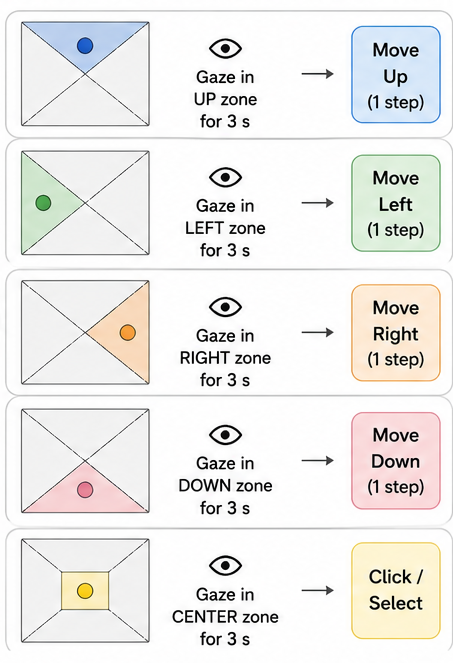
\includegraphics[width=200]{figures/ch08/fig4_latex.png}
\label{fig:system3}
\end{figure}

\newpage

This system was a significant improvement over Iteration~2 in two respects:

\begin{itemize}
    \item \textbf{Dramatic reduction in false positives:} Natural blinks had no effect
    whatsoever, as the system only measured sustained gaze position, not eye closure events.
    \item \textbf{Reduced fatigue:} Users no longer needed to consciously count or time
    blinks. Simply looking in a direction was enough.
\end{itemize}

However, two new failure modes emerged:

\begin{itemize}
    \item \textbf{Dwell-while-reading false triggers:} Users frequently dwell in a screen
    region for more than 3 seconds simply because they are \textit{reading} content in that
    area of the display. A user reading text in the lower-right of the screen would
    inadvertently trigger a \textit{right} or \textit{down} movement while doing nothing
    other than reading. This produced unexpected motion and was disorienting.

    \item \textbf{Low throughput for compound actions:} Executing any non-trivial task
    required many sequential dwell steps. For instance, navigating from the home screen to
    a specific destination required multiple \textit{right}/\textit{down} steps, each
    costing at least 3 seconds of deliberate gaze. Complex actions became slow and tiring.
\end{itemize}

The five-zone system was rejected, but its core insight — that dwell-based selection is
far superior to blink counting for ALS users — was carried into the fourth iteration.

% ......................................
\subection{Iteration 4 — Edge-Popup Dwell Buttons (Selected)}
% ......................................

The fourth and final design retained dwell-based selection but fundamentally restructured
how commands are presented and triggered. Instead of dividing the entire screen into
navigation zones (which conflicted with reading), \textbf{eight action buttons} are placed
at the edges and corners of the screen — invisible during normal use and appearing only when
the user's gaze deliberately approaches the screen periphery (within 18\% of any edge).

\begin{figure}[H]
\centering
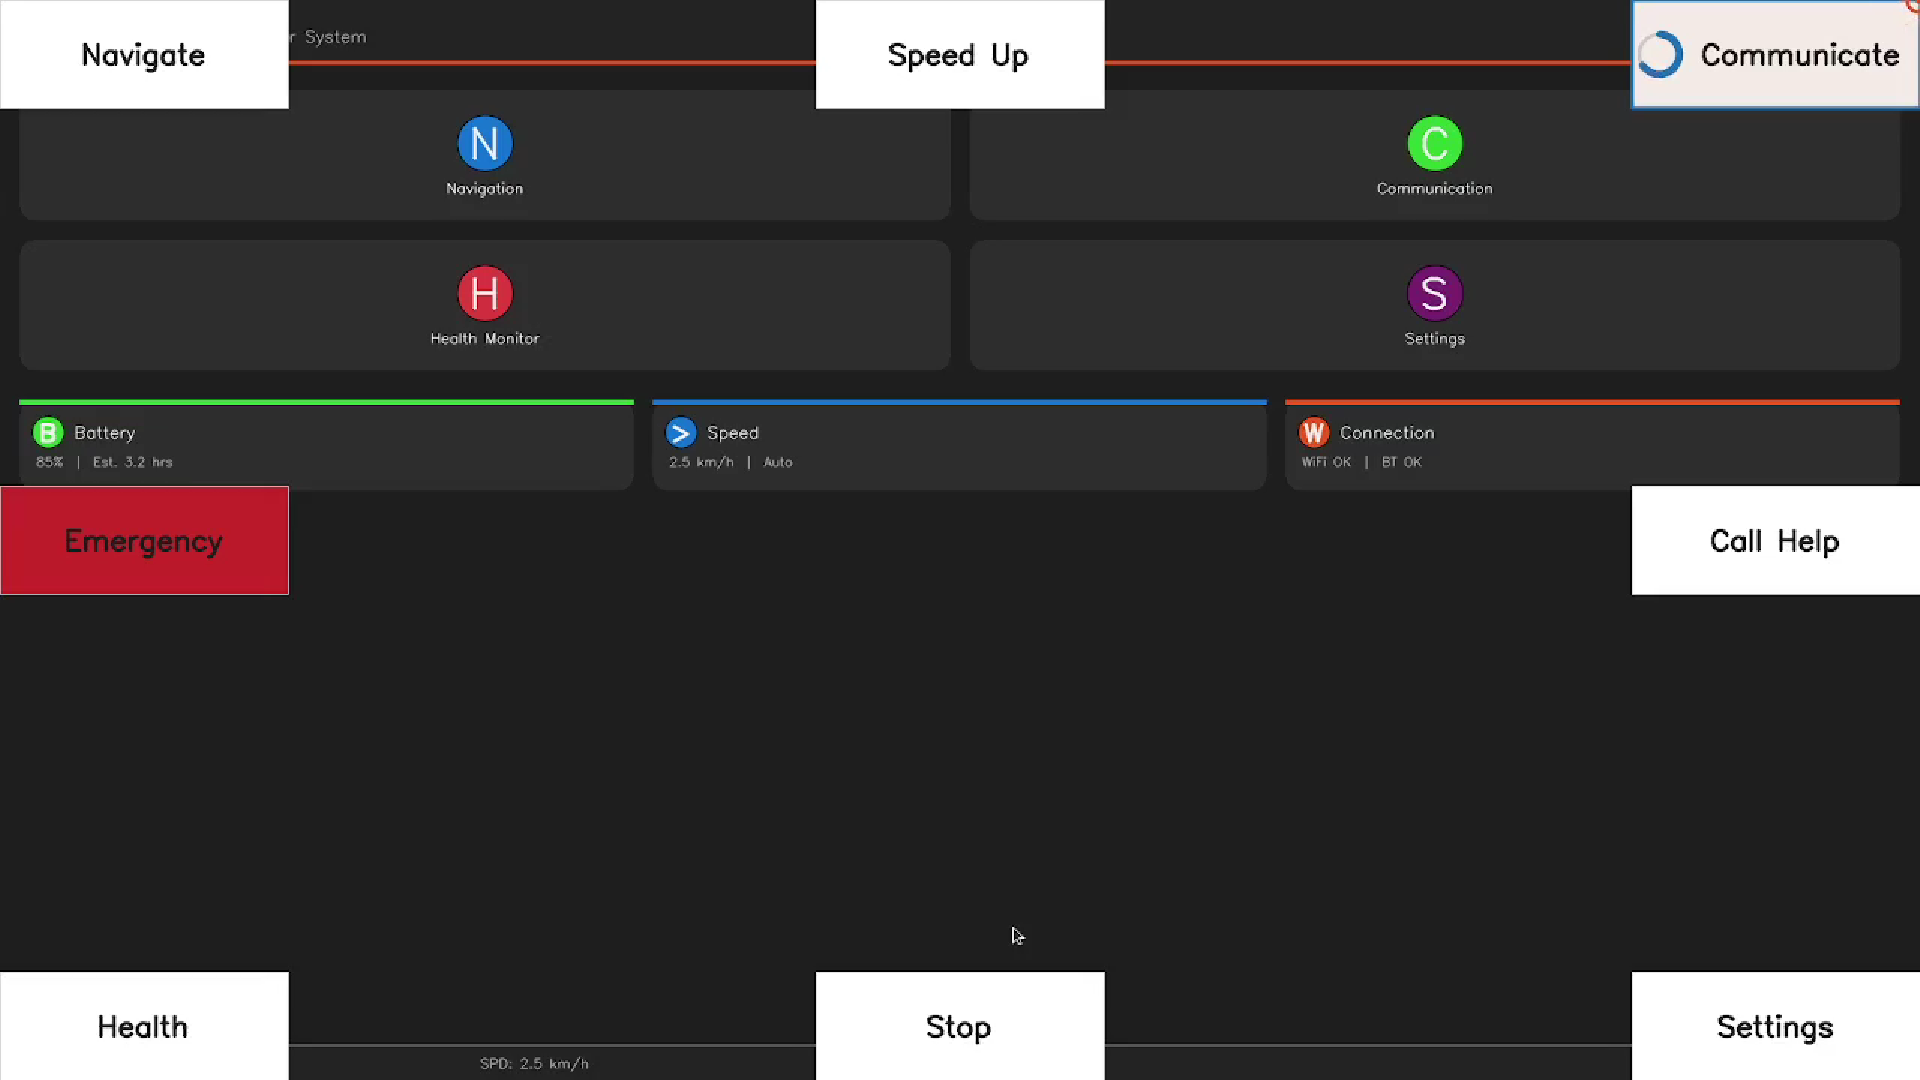
\includegraphics[width=450]{figures/ch08/fig6_latex.png}
\label{fig:system4}
\end{figure}

\begin{figure}[H]
\centering
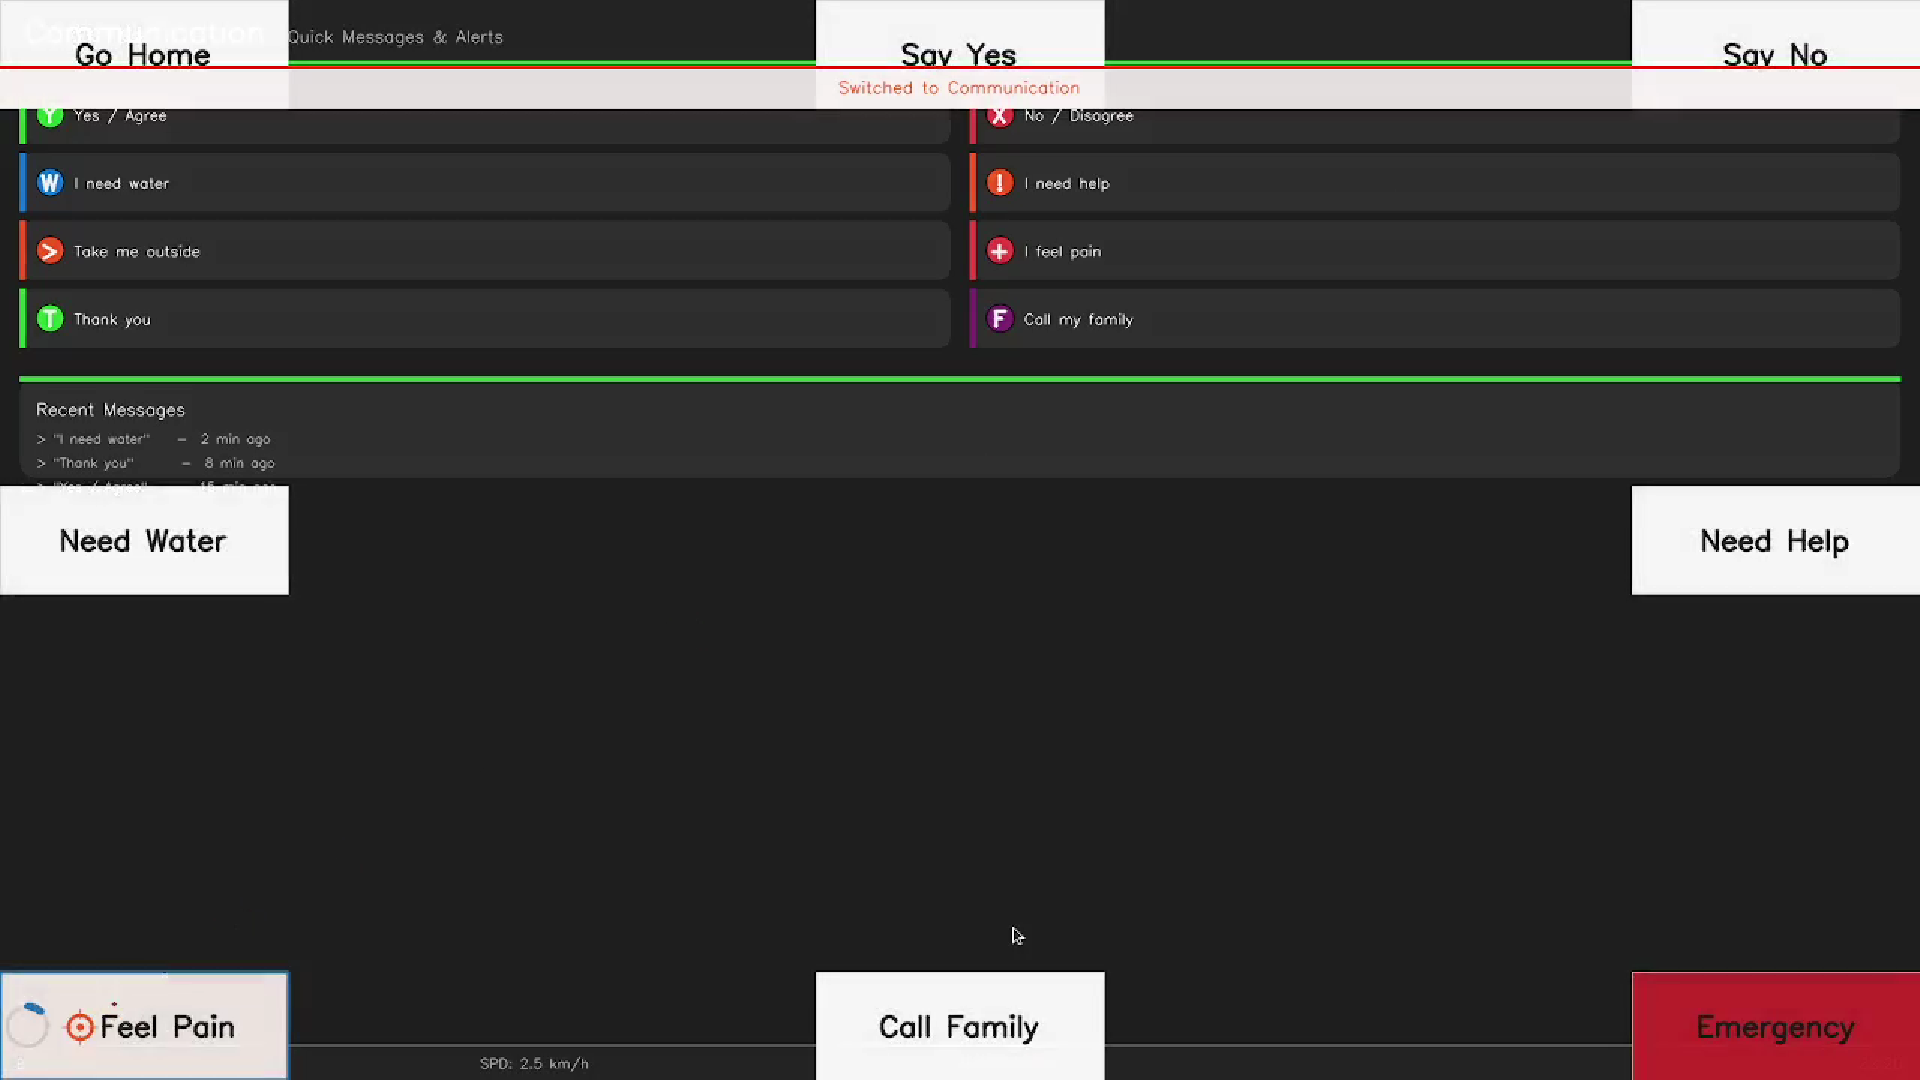
\includegraphics[width=450]{figures/ch08/fig7_latex.png}
\caption{The Selected Gaze Command Control system in action.}
\label{fig:system4_1}
\end{figure}

This design addressed both failure modes from Iteration~3:

\begin{itemize}
    \item \textbf{No false triggers while reading:} The central 82\% of the screen contains
    no interactive elements. A user reading content anywhere in that area cannot accidentally
    trigger a command regardless of how long they dwell there.

    \item \textbf{Context-sensitive actions:} Each of the  application screens (Home,
    Navigation, Communication, Health Monitor, Settings, ...etc) defines its own set of eight button
    labels. The most crucial seven actions for that specific screen are always one dwell
    away, dramatically reducing the number of steps needed per task compared to
    Iteration~3's sequential navigation model.

    \item \textbf{Reduced dwell time:} Because each button maps directly to a meaningful
    action rather than a single step, the dwell threshold reduced from 3 to 2 seconds
    without increasing false positives, making the interface 33.33 percent  faster.
\end{itemize}
When gaze enters the edge zone, the corresponding buttons fade in smoothly (4--5 frame
transition at 30~fps). During a dwell, a \textbf{progress slider} sweeps around the
button from start to end of the button, giving the user continuous visual feedback of progress toward
activation. A 0.6~s cooldown after each activation prevents unintended double-firing.
Sustained eye closure ($\geq$~2.0~s) is preserved as a universal \textit{back/cancel}
command across all screens, handled by the \texttt{gaze\_controller\_node}.

% ......................................
\subection{Interaction Design Comparison Summary}
% ......................................

Table~\ref{tab:et_interaction_comparison} summarises all four iterations across the
key evaluation criteria used to guide each design decision.

\begin{table}[H]
\centering
\caption{Gaze Interaction Design Iteration Comparison}
\label{tab:et_interaction_comparison}
\begin{tabular}{p{2.8cm}p{3.2cm}p{2.6cm}p{3.2cm}p{1.6cm}}
\toprule
\textbf{System} & \textbf{Mechanism} & \textbf{Advantages} & \textbf{Failure Mode} & \textbf{Decision} \\
\midrule
Iteration 1 \newline Hand Gestures
  & Camera-based gesture recognition
  & Mature technology; rich vocabulary
  & Requires functioning hands; incompatible with ALS target users
  & Rejected \\[6pt]

Iteration 2 \newline Blink-Coded
  & Blink count sequences (e.g.\ 2 blinks = right, 3 = left, 3\,s closure = confirm)
  & Eyes-only; no gaze tracking required
  & Severe false positives from natural blinks; eye fatigue; dry eyes; high cognitive load
  & Rejected \\[6pt]

Iteration 3 \newline Five-Zone Frame
  & Screen divided into 5 dwell regions via diagonals; 3\,s dwell per step; 3\,s closure = back
  & No blink false positives; low fatigue
  & False triggers while reading; low throughput (many steps per task)
  & Rejected \\[6pt]

\textbf{Iteration 4} \newline \textbf{Edge-Popup Dwell}
  & 8 context-sensitive buttons at screen edges; appear only when gaze nears periphery; 3\,s closure = back
  & \textbf{No false triggers while reading; context-sensitive actions; reduced dwell time; fast task completion}
  & Requires accurate gaze to reach edges reliably
  & \textbf{Selected} \\
\bottomrule
\end{tabular}
\end{table}

% ......................................
\subsection{Final Implementation: ROS 2 Command Node}
% ......................................
The \texttt{gaze\_controller\_node} subscribes to \texttt{/eye\_tracking/eye\_state} and
    implements a three-state machine to handle the eye-closure back command. 
    \begin{itemize}
        \item While the eye is
        \texttt{"open"}, the cursor tracks the live gaze position. 
        \item A \texttt{"blink"} event freezes
        the cursor and resets the closure timer. 
        \item Sustained \texttt{"closed"} state for
        $\geq$~2.0~s emits a \texttt{"click"} command on \texttt{/eye\_tracking/command}, followed
        by a 0.6~s cooldown to prevent repeat triggers. 
\end{itemize}
This mechanism handles back/cancel and
confirm actions at the system level, while all directional and screen-specific actions are handled by the edge-popup dwell system in the touchscreen UI layer.

% ----------------------------------------------------------------
\section{Gaze Pipeline Diagram}
% ----------------------------------------------------------------
The eye-tracking pipeline is divided into two ROS 2 nodes. The eye\_tracker\_node acquires camera frames, estimates the user's gaze using MediaPipe and iris-based processing, and publishes the gaze position and eye state. The gaze\_controller\_node subscribes to these topics, executes the command state machine to interpret user intent (tracking, blink, or sustained eye closure), and generates the corresponding control commands for the wheelchair.

\begin{figure}[H]
\centering
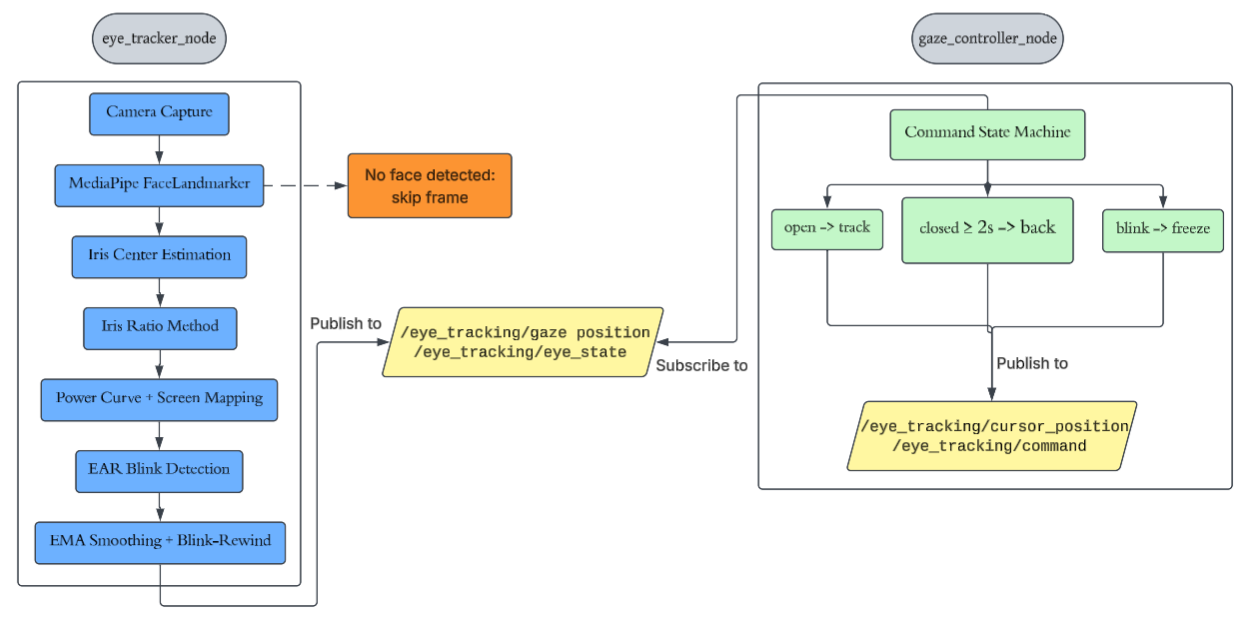
\includegraphics[width=475]{figures/ch08/the_diagram}
\caption{Sanad eye tracking pipeline: from camera capture to ROS~2 command dispatch.
Red dashed arrows indicate exception paths.}
\label{fig:gaze_pipeline}
\end{figure}



% ----------------------------------------------------------------
\section{System Performance and Observations}
% ----------------------------------------------------------------

At the current stage of the project, formal quantitative evaluation of gaze accuracy — such
as controlled angular error measurements or statistically significant success-rate trials —
has not yet been conducted. A structured user study with participants representing the target
population is planned as part of the testing phase. The observations
reported here reflect the development team's experience operating the system under realistic
indoor conditions during integration and functional testing.

\textbf{General responsiveness:} The pipeline runs at a stable 20--28 inference frames per
second on the Raspberry Pi~4 without any GPU acceleration. The end-to-end latency from eye
movement to cursor update is approximately 57--65~ms, which is imperceptible to the user
and well within the 200~ms threshold at which humans begin to notice interface lag.
The cursor feels immediate and natural to operate.

\textbf{Gaze tracking stability:} Under standard indoor lighting conditions, the
MediaPipe FaceLandmarker model tracks the iris consistently without dropout, and the EMA
smoothing ($\alpha = 0.30$) eliminates visible cursor jitter while preserving
responsiveness to deliberate gaze shifts. The blink-rewind buffer successfully prevents the
cursor from drifting downward during natural blinks, which was a noticeable artefact in
early testing before the buffer was introduced.

\textbf{Dwell activation reliability:} The edge-popup buttons activate reliably when gaze
is held intentionally at a screen edge. No false activations were observed during normal
reading or resting gaze within the central screen area, confirming that the 18\% edge-trigger
threshold effectively separates intentional peripheral gaze from passive content viewing.

\textbf{Eye-closure command:} The 2-second sustained closure threshold for back/confirm
commands proved comfortable in practice. Natural blinks (typically 150--400~ms in
duration) never triggered the command, and intentional closures were
consistently recognised without requiring excessive effort from the operator.

\textbf{Computational headroom:} CPU usage across both nodes remains within 30--45\% of a
single Pi~4 core, leaving the remaining processing capacity fully available for the
concurrent touchscreen interface, ROS~2 middleware, and other Sanad subsystems running on
the same board.

Formal accuracy benchmarking, including gaze-point error under varying lighting conditions and multi-session dwell success rates, remains as future work.

\section{Summary and Transition}
This chapter has detailed the webcam-based eye-gaze tracking pipeline, which enables hands-free system navigation and interaction. The next chapter, Chapter 9 (Mobile Application), extends control to the user's care network by detailing the cross-platform application designed for remote monitoring and diagnostics.



\chapterseparator{Chapter 9}
\setcounter{chapter}{9} 
\chapter*{Chapter (9): Mobile Application}
\addcontentsline{toc}{chapter}{Chapter (9): Mobile Application} 
\renewcommand{\thesection}{\thechapter.\arabic{section}}
\setcounter{section}{0}
\captionsetup[figure]{justification=centering}

\section{Chapter Preview}
This chapter presents the design and features of the caregiver-focused mobile application. It outlines the NativeWind-styled React Native and Expo framework selection, details the biometric telemetry stream and Telegram-based emergency alerts, and explains the remote smart-home and diagnostic control interfaces.

Usability is the core focus of the mobile interface. Caregivers must be able to quickly read critical physiological data and check system alerts with minimal latency. High-contrast indicators and a clear visual hierarchy are implemented to make operation reliable under stress or in low-visibility environments. Table \ref{tab:mobile-requirements} lists the primary functional and non-functional requirements of the mobile app.

\begin{table}[H]
\centering
\caption{Mobile Application Functional and Non-Functional Requirements}
\label{tab:mobile-requirements}
\begin{tabularx}{\textwidth}{|l|>{\raggedright\arraybackslash}X|c|}
\hline
\textbf{Req. ID} & \textbf{Requirement Description} & \textbf{Priority} \\ \hline
FR-01 & Authenticate caregivers and securely link their accounts to the patient's Telegram session. & Must \\ \hline
FR-02 & Monitor patient biometrics (temperature and heart rate) in real time. & Must \\ \hline
FR-03 & Trigger automatic alert notifications to designated Telegram chats during biometric emergencies. & Must \\ \hline
FR-04 & Control smart home devices in the patient's environment (lights, dimmers, locks). & Should \\ \hline
FR-05 & Monitor system diagnostics (battery state, speed limits, controller CPU temperature). & Should \\ \hline
NFR-01 & Minimize latency: Notification transmission delay must remain under 100 ms. & Must \\ \hline
NFR-02 & Accessibility: Support screen readers and high-contrast styling. & Should \\ \hline
NFR-03 & Interface flexibility: Provide dark and light modes for different environment illumination. & Should \\ \hline
\end{tabularx}
\end{table}

\begin{figure}[H]
\centering
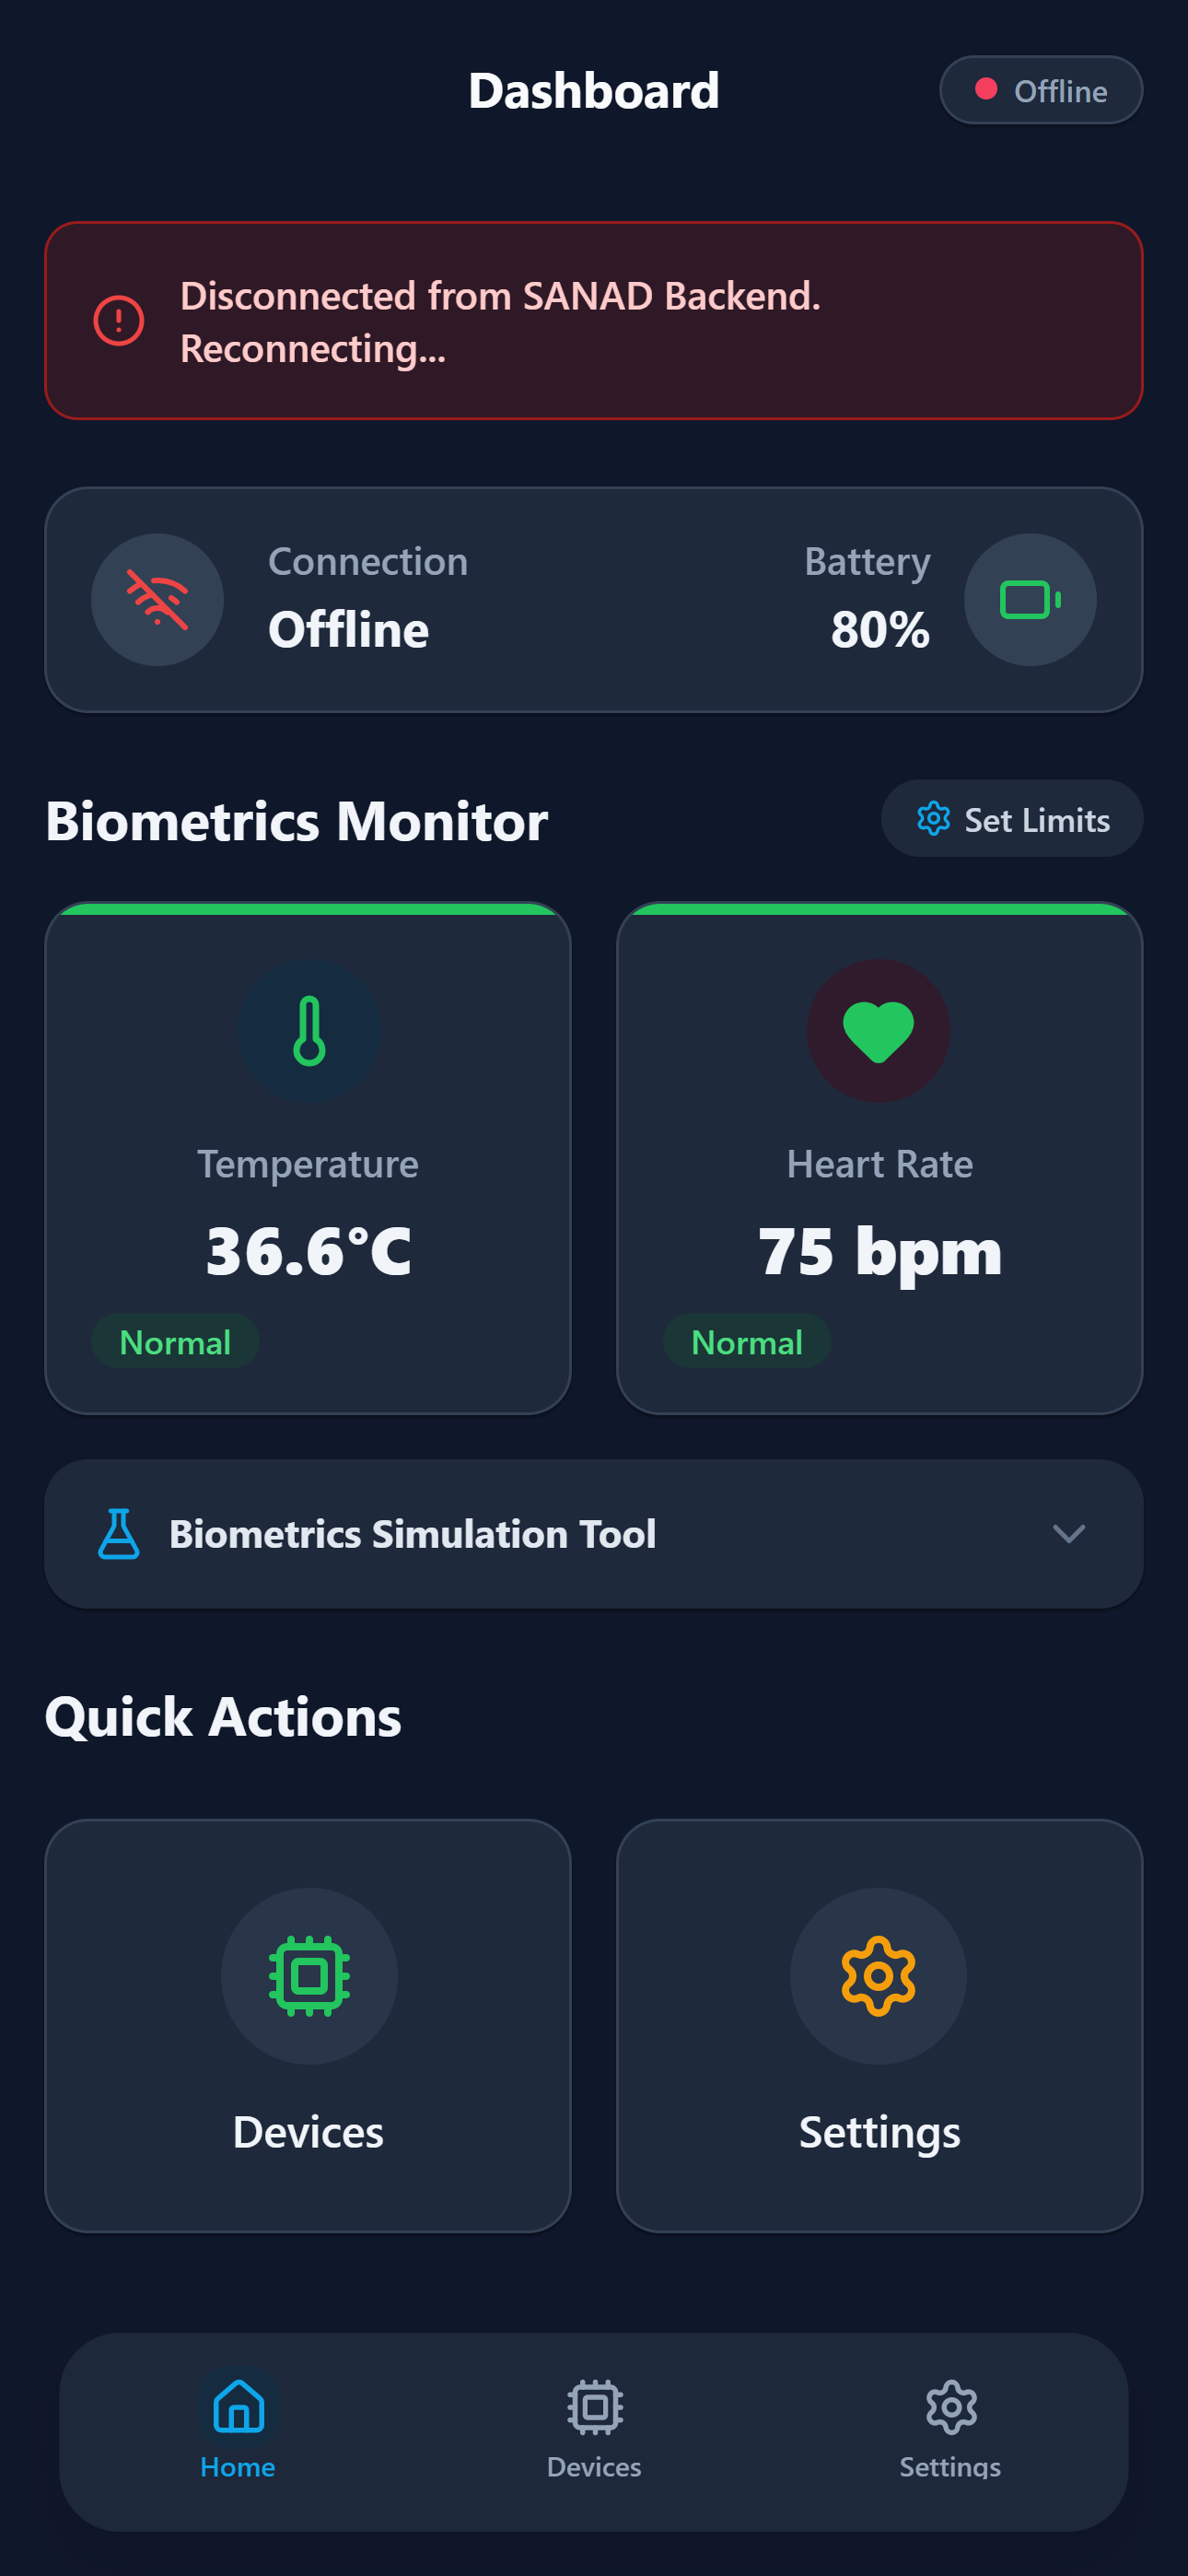
\includegraphics[width=0.45\textwidth]{figures/ch09/mobile_overview.png}
\caption{Main dashboard view of the SANAD mobile application showing active telemetry and biometrics status.}
\label{fig:mobile-overview}
\end{figure}

\section{Technology Stack \& Native Alternatives}
To target both Android and iOS devices from a single codebase, a cross-platform mobile framework was necessary. During the initial design, multiple options were evaluated, including native development, Flutter, progressive web applications (PWAs), and React Native.

\textbf{React Native} was chosen, utilizing the \textbf{Expo} framework (version 54) and \textbf{TypeScript}. React Native compiles to native platform components, ensuring smooth rendering performance and native responsiveness, unlike hybrid WebView-based alternatives. Expo simplifies access to device hardware and provides a clean development workflow. \textbf{NativeWind 4} is used for styling, bringing Tailwind's utility-first class model to React Native.

Table \ref{tab:mobile-frameworks} compares the evaluated mobile frameworks.

\begin{table}[H]
\centering
\caption{Mobile Framework Evaluation Metrics}
\label{tab:mobile-frameworks}
\begin{tabularx}{\textwidth}{|>{\raggedright\arraybackslash}X|c|c|c|}
\hline
\textbf{Metric} & \textbf{React Native (Expo)} & \textbf{Flutter} & \textbf{PWA / WebView} \\ \hline
Development Velocity & Very High & High & High \\ \hline
Code Reusability & > 90\% & > 90\% & 100\% \\ \hline
Bundle Size (Base) & \textasciitilde 22 MB & \textasciitilde 15 MB & < 2 MB \\ \hline
Haptics API Access & Native Wrapper & Native Wrapper & Limited \\ \hline
Layout Engine & Yoga (Flexbox) & Skia Canvas & HTML DOM \\ \hline
\end{tabularx}
\end{table}

Key dependencies in the mobile project include:
\begin{itemize}
    \item \textbf{socket.io-client}: Manages the persistent WebSocket connection to the Node.js server for real-time telemetry.
    \item \textbf{react-native-gesture-handler} \& \textbf{react-native-reanimated}: Powers the interactive elements, such as slide-up panels and smooth drawer transitions.
    \item \textbf{expo-haptics}: Provides physical haptic feedback during alert and emergency events.
    \item \textbf{react-native-toast-message}: Displays overlay notifications for system warnings and connection status changes.
\end{itemize}

\section{Application Architecture \& Routing}
The mobile application uses the \textbf{group-by-feature} directory structure to keep related code modules organized.
The navigation structure is powered by \textbf{Expo Router}. The root layout (\texttt{app/\_layout.tsx}) initializes global connection contexts and checks the user's authentication state. If the user is unauthenticated, they are redirected to the login screen. Once logged in, the app loads the tab navigator (\texttt{app/(tabs)/\_layout.tsx}), which configures the bottom navigation bar and displays the server connection status (Connected/Offline) in the top-right header.


\section{Mobile-to-Server Communication Architecture}
The SANAD mobile application operates as a remote HMI (Human-Machine Interface) for caregivers and medical personnel. To support seamless remote observation, the mobile application establishes two distinct communication channels with the Node.js server. This architecture separates high-frequency telemetry from transactional controls, preventing connection congestion and ensuring that physiological alerts are dispatched and received with sub-second latencies.

\subsection{Communication Topology}
The networking layout of the mobile monitoring system is divided into the client-side presentation layer (React Native mobile application and Telegram client), the supervisory layer (Node.js server), and the execution layer (onboard ROS 2 bridge and smart home appliances). Figure \ref{fig:mobile-server-comm-tikz} shows the network topology and the specific protocol pathways connecting these subsystems.

\begin{figure}[H]
\centering
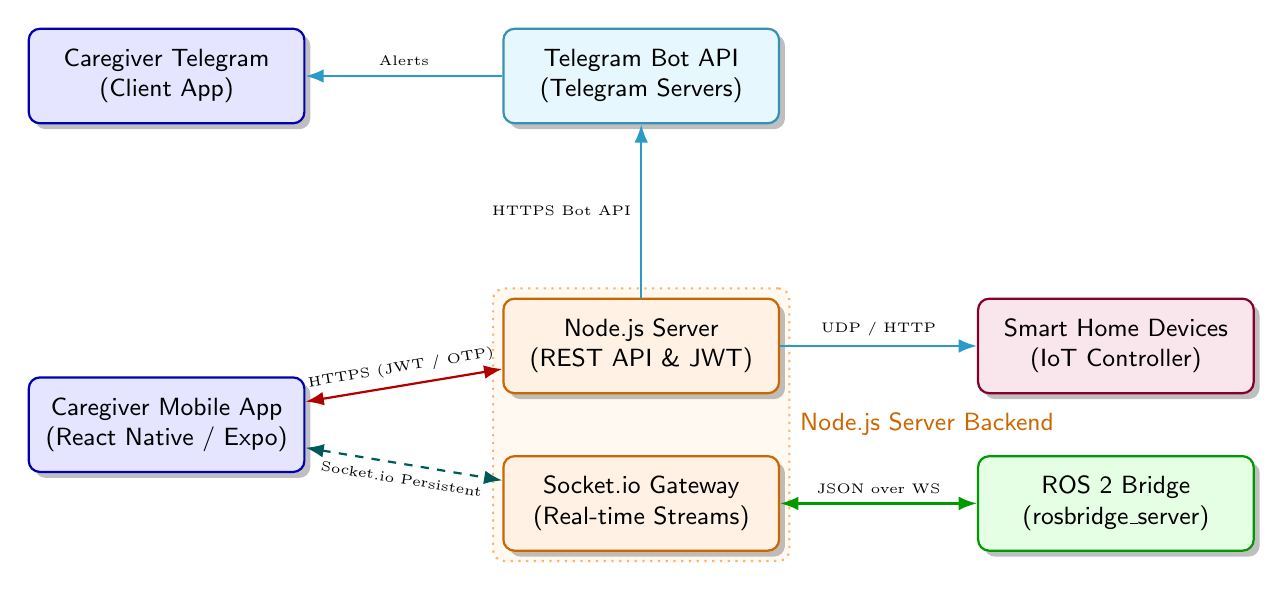
\begin{tikzpicture}[
    font=\sffamily\small,
    node distance=2.2cm and 2.5cm,
    clientNode/.style={rectangle, draw=blue!70!black, fill=blue!10, rounded corners, minimum width=3.5cm, minimum height=1.2cm, align=center, thick, drop shadow},
    serverNode/.style={rectangle, draw=orange!80!black, fill=orange!10, rounded corners, minimum width=3.5cm, minimum height=1.2cm, align=center, thick, drop shadow},
    hardwareNode/.style={rectangle, draw=green!60!black, fill=green!10, rounded corners, minimum width=3.5cm, minimum height=1.2cm, align=center, thick, drop shadow},
    telegramNode/.style={rectangle, draw=cyan!70!black, fill=cyan!10, rounded corners, minimum width=3.5cm, minimum height=1.2cm, align=center, thick, drop shadow},
    iotNode/.style={rectangle, draw=purple!70!black, fill=purple!10, rounded corners, minimum width=3.5cm, minimum height=1.2cm, align=center, thick, drop shadow},
    httpArrow/.style={Latex-Latex, draw=red!70!black, thick},
    wsArrow/.style={Latex-Latex, draw=teal!70!black, dashed, thick},
    apiArrow/.style={-Latex, draw=cyan!80!black, thick},
    rosArrow/.style={Latex-Latex, draw=green!60!black, thick}
]

    \node[clientNode] (mobile) {Caregiver Mobile App\\(React Native / Expo)};
    
    \node[serverNode, right=of mobile, yshift=1cm] (nodejs) {Node.js Server\\(REST API \& JWT)};
    \node[serverNode, right=of mobile, yshift=-1cm] (socketio) {Socket.io Gateway\\(Real-time Streams)};
    
    \node[telegramNode, above=of nodejs] (tgBot) {Telegram Bot API\\(Telegram Servers)};
    \node[clientNode, left=of tgBot] (tgClient) {Caregiver Telegram\\(Client App)};
    
    \node[hardwareNode, right=of socketio] (rosbridge) {ROS 2 Bridge\\(rosbridge\_server)};
    \node[iotNode, right=of nodejs] (iot) {Smart Home Devices\\(IoT Controller)};

    \begin{scope}[on background layer]
        \node[draw=orange!60, fill=orange!5, dotted, thick, rounded corners, fit=(nodejs) (socketio), label={[orange!80!black]right:Node.js Server Backend}] (serverGroup) {};
    \end{scope}

    \draw[httpArrow] (mobile) -- node[above, sloped, font=\tiny] {HTTPS (JWT / OTP)} (nodejs);
    \draw[wsArrow] (mobile) -- node[below, sloped, font=\tiny] {Socket.io Persistent} (socketio);
    
    \draw[apiArrow] (nodejs) -- node[left, font=\tiny] {HTTPS Bot API} (tgBot);
    \draw[apiArrow] (tgBot) -- node[above, font=\tiny] {Alerts} (tgClient);
    
    \draw[rosArrow] (socketio) -- node[above, font=\tiny] {JSON over WS} (rosbridge);
    \draw[apiArrow] (nodejs) -- node[above, font=\tiny] {UDP / HTTP} (iot);

\end{tikzpicture}
\caption{Communication topology of the mobile monitoring system, showing REST and Socket.io transport channels between the React Native client, Node.js server, Telegram services, and ROS 2 execution stack.}
\label{fig:mobile-server-comm-tikz}
\end{figure}

\subsection{REST API and Stateless Interventions}
Stateless and transactional operations are handled through standard HTTPS request-response cycles. These transactions include caregiver registration and authentication, generation and validation of Telegram session tokens, smart home device network discovery queries, and profile configuration adjustments. In compliance with security standards, all transactional endpoints are protected by JSON Web Token (JWT) verification, requiring the client to pass the bearer token in the HTTP Authorization header. This channel is also subject to strict schema validation on the backend to filter out malformed requests before they trigger database queries.

\subsection{Socket.io persistent Telemetry Channel}
For streaming real-time biometric diagnostics and system health updates, the mobile application maintains a persistent connection via the Socket.io protocol (a layer built on top of TCP WebSockets). This persistent, full-duplex socket allows the Node.js server to push new biometric metrics (heart rate, body temperature) and diagnostic values (onboard CPU temperature, speed limit modifiers, battery percentages) to the client as soon as they are received from the ROS 2 bridge. This architecture eliminates the processing and network overhead of traditional HTTP polling, ensuring that the caregiver's dashboard displays real-time patient states.

\subsection{ROS-to-Web Message Mapping}
The Node.js server functions as a message aggregator and translator. It maintains a persistent WebSocket connection to the onboard \texttt{rosbridge\_server}, subscribing to native ROS 2 topics and publishing commands. When ROS 2 messages are received, the server extracts the raw payload values and maps them directly to corresponding Socket.io events. To guarantee type compatibility, the mobile client connection provider translates raw socket JSON responses into standardized ROS message schemas, such as representing coordinates as a ROS \texttt{PoseWithCovarianceStamped} structure before passing them to client-side callback hooks.

\subsection{Connection Resiliency and Heartbeats}
To handle network disruptions, the mobile application integrates a connection provider that manages socket state lifecycles:
\begin{itemize}
    \item \textbf{Heartbeat Loop}: The mobile client exchanges periodic keep-alive ping-pong packages with the Node.js gateway. If no response is received within $2500\text{ ms}$, the connection is marked as disconnected.
    \item \textbf{Visual Notification}: The application displays a warning banner and changes the status indicator in the tab header to "Offline" to alert the caregiver.
    \item \textbf{Exponential Reconnection}: The client automatically attempts to re-establish the Socket.io connection using an exponential backoff algorithm (reconnecting every $5\text{ seconds}$ initially, and scaling up to $30\text{ seconds}$ to conserve mobile battery).
    \item \textbf{Local Cache Persistency}: While disconnected, the application caches local parameters (such as the last targeted Telegram chat ID and base connection URLs) in local persistent storage, restoring the client to a functional state immediately once connectivity is re-established.
\end{itemize}


\section{Biometrics Monitor \& Alarm Pipeline}
Patient safety is a key priority for the SANAD system. The mobile application features a real-time \textbf{Biometrics Monitor} (\texttt{HomeScreen}) that tracks the patient's body temperature and heart rate.

\subsection{Metrics Processing \& Fluctuation}
In the current implementation, biometric telemetry is processed in real time. To account for live physiological changes, a background timer in the \texttt{useBiometrics.ts} hook fluctuates values every 3 seconds:
\begin{align}
T_{t+1} &= T_t + \delta_T - 0.15 \cdot (T_t - T_{\text{baseline}}) \\
\text{HR}_{t+1} &= \text{HR}_t + \delta_{\text{HR}} - 0.15 \cdot (\text{HR}_t - \text{HR}_{\text{baseline}})
\end{align}
where $T_{\text{baseline}} = 36.6^{\circ}\text{C}$ and $\text{HR}_{\text{baseline}} = 75\text{ bpm}$. The random steps $\delta_T \in [-0.06, 0.06]$ and $\delta_{\text{HR}} \in [-1, 1]$ represent natural variations, while the proportional feedback term pulls the metrics back toward the baseline to prevent drift.

\subsection{Threshold Alarms}
Caregivers can set custom safety ranges for the patient's biometrics using slider controls:
\begin{itemize}
    \item \textbf{Temperature Limits}: Min temperature ($34.5^{\circ}\text{C} \dots 36.5^{\circ}\text{C}$), Max temperature ($37.0^{\circ}\text{C} \dots 39.0^{\circ}\text{C}$).
    \item \textbf{Heart Rate Limits}: Min heart rate ($40 \dots 75\text{ bpm}$), Max heart rate ($85 \dots 130\text{ bpm}$).
\end{itemize}

If a patient's metrics cross these thresholds, the state machine triggers an emergency alert. The app displays a local warning banner, sends a system notification, and dispatches an alert message to the caregiver's Telegram account. When the metrics return to normal, the system automatically sends a resolution update, keeping the caregiver informed.

\begin{figure}[H]
\centering
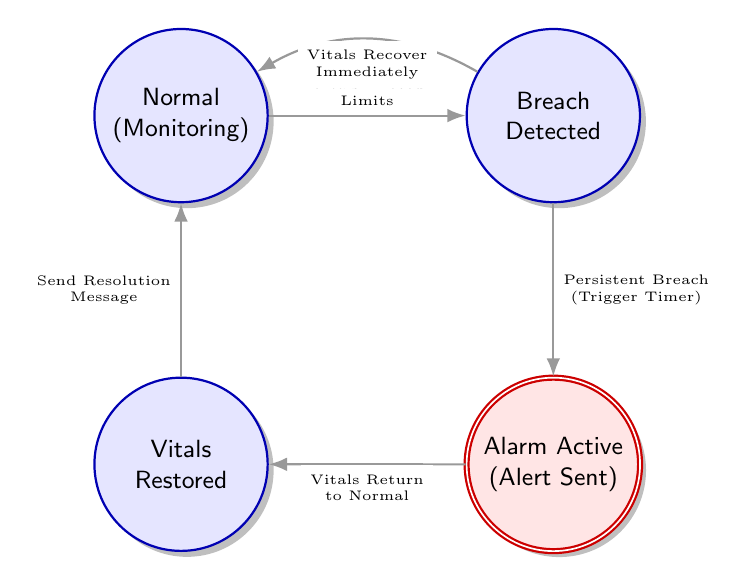
\begin{tikzpicture}[
    font=\sffamily\small,
    node distance=2.2cm and 2.5cm,
    state/.style={circle, draw=blue!70!black, fill=blue!10, thick, minimum size=2.2cm, align=center, drop shadow},
    activeState/.style={circle, draw=red!80!black, fill=red!10, thick, minimum size=2.2cm, align=center, double, drop shadow},
    arrow/.style={-Latex, thick, draw=gray!80},
    transLabel/.style={font=\tiny, fill=white, align=center}
]

    % States
    \node[state] (normal) {Normal\\(Monitoring)};
    \node[state, right=of normal] (breach) {Breach\\Detected};
    \node[activeState, below=of breach] (alarm) {Alarm Active\\(Alert Sent)};
    \node[state, below=of normal] (resolve) {Vitals\\Restored};

    % Transitions
    \draw[arrow] (normal) -- node[above, transLabel] {Vitals Exceed\\Limits} (breach);
    \draw[arrow] (breach) -- node[right, transLabel] {Persistent Breach\\(Trigger Timer)} (alarm);
    
    % Breach to Normal (False alarm / transient)
    \draw[arrow, bend right=30] (breach) to node[below, transLabel] {Vitals Recover\\Immediately} (normal);
    
    % Alarm to Resolve
    \draw[arrow] (alarm) -- node[below, transLabel] {Vitals Return\\to Normal} (resolve);
    
    % Resolve to Normal
    \draw[arrow] (resolve) -- node[left, transLabel] {Send Resolution\\Message} (normal);

\end{tikzpicture}
\caption{State machine diagram illustrating the biometrics monitor alarm pipeline lifecycle.}
\label{fig:biometrics-alarm-state-machine}
\end{figure}

\begin{figure}[H]
\centering
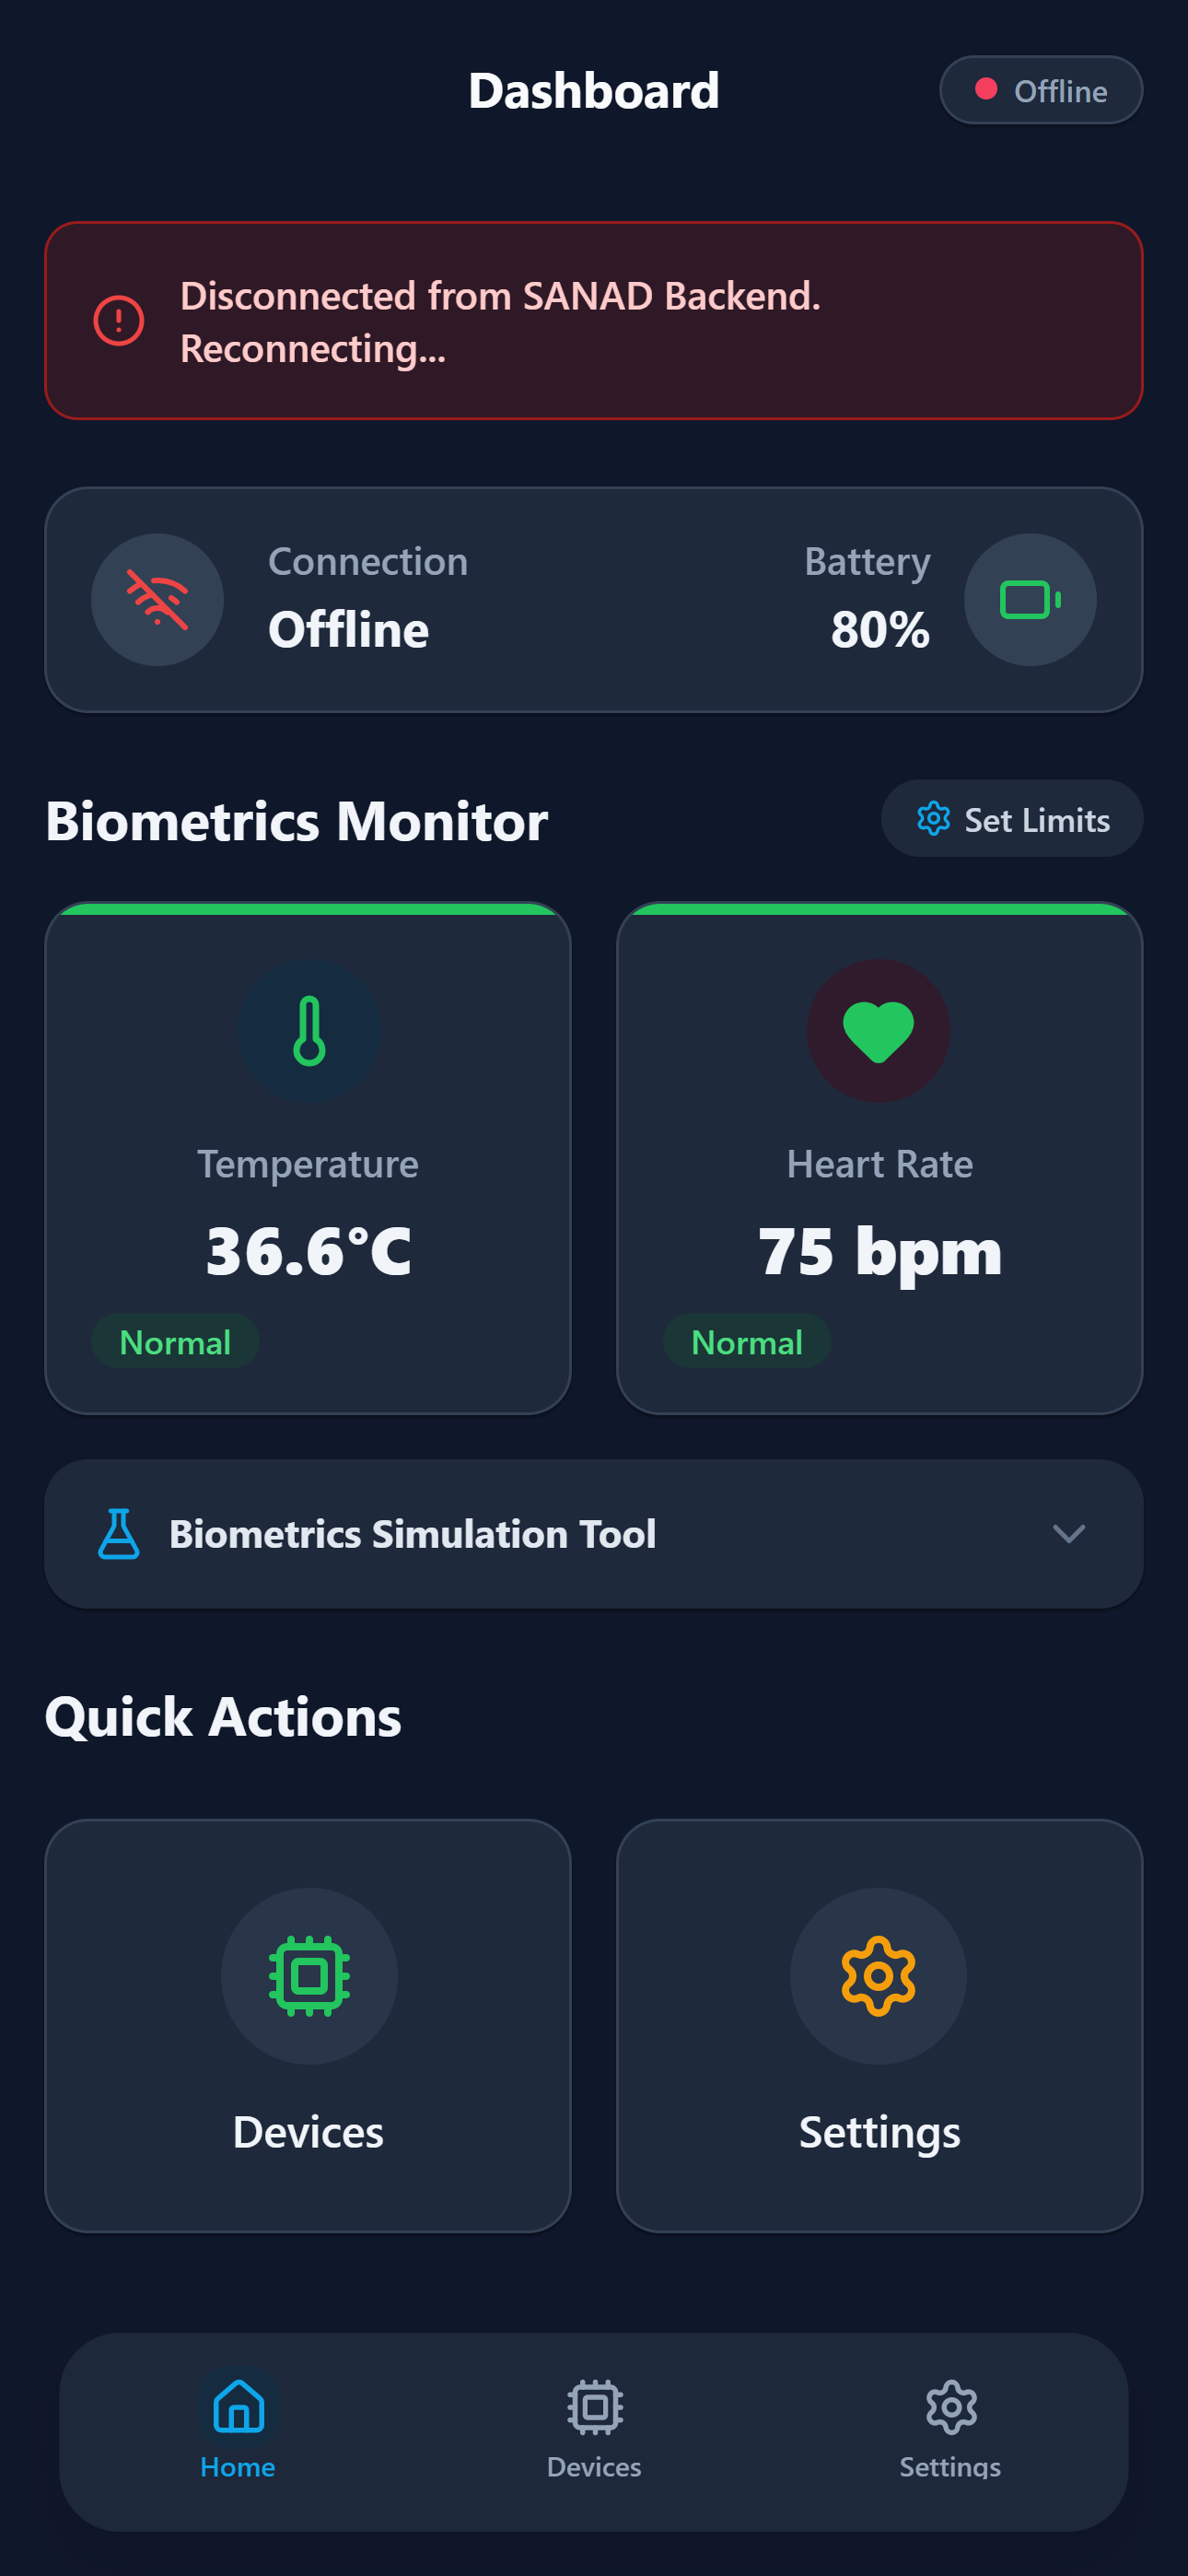
\includegraphics[width=0.48\textwidth]{figures/ch09/biometrics_cards.png}
\caption{Real-time Biometrics dashboard cards showing temperature and heart rate metrics with status badges.}
\label{fig:biometrics-cards}
\end{figure}

\section{Telegram Alert Integration \& Destination Matching}
To deliver alerts even when the mobile app is closed, the system integrates with the Telegram Bot API. 

When the biometrics monitor detects a threshold breach, it dispatches the alert message using the Telegram service wrapper. The backend bot then forwards the alert to the selected recipient. Caregivers can configure the alert destination in the settings panel, choosing between:
\begin{itemize}
    \item \textbf{Saved Messages (Me)}: Sends alerts directly to the caregiver's personal Telegram chat.
    \item \textbf{Group Dialogs}: Sends alerts to a shared family or medical Telegram group.
\end{itemize}

The list of available chats is fetched from the Telegram client API using the user's ID by querying the registered users and groups endpoints on the backend. The selected chat ID is saved locally on the device using \texttt{AsyncStorage} under the key \texttt{"@sannad\_biometric\_target\_chat"}. This ensures alert routing preferences persist across app restarts.

\begin{figure}[H]
\centering

\includegraphics[width=0.5\textwidth]{figures/ch09/telegram_alert_msg.png}
\caption{Caregiver's phone screen showing a real-time emergency alert message received via the Telegram Bot.}
\label{fig:telegram-alert-msg}
\end{figure}

\section{Smart Home \& Device Discovery}
The Smart Home view (\texttt{smart-home.tsx}) allows caregivers to control IoT devices in the patient's room from their mobile phone.

Discovered smart devices are grouped and displayed by room. Caregivers can toggle devices (like lights and TVs) using switch widgets. If no devices are detected, the app displays an empty state illustration with a "Discover Devices" button. Clicking this sends a scan request to the server, which runs a UDP broadcast to discover active devices and update the local list.

\begin{figure}[H]
\centering
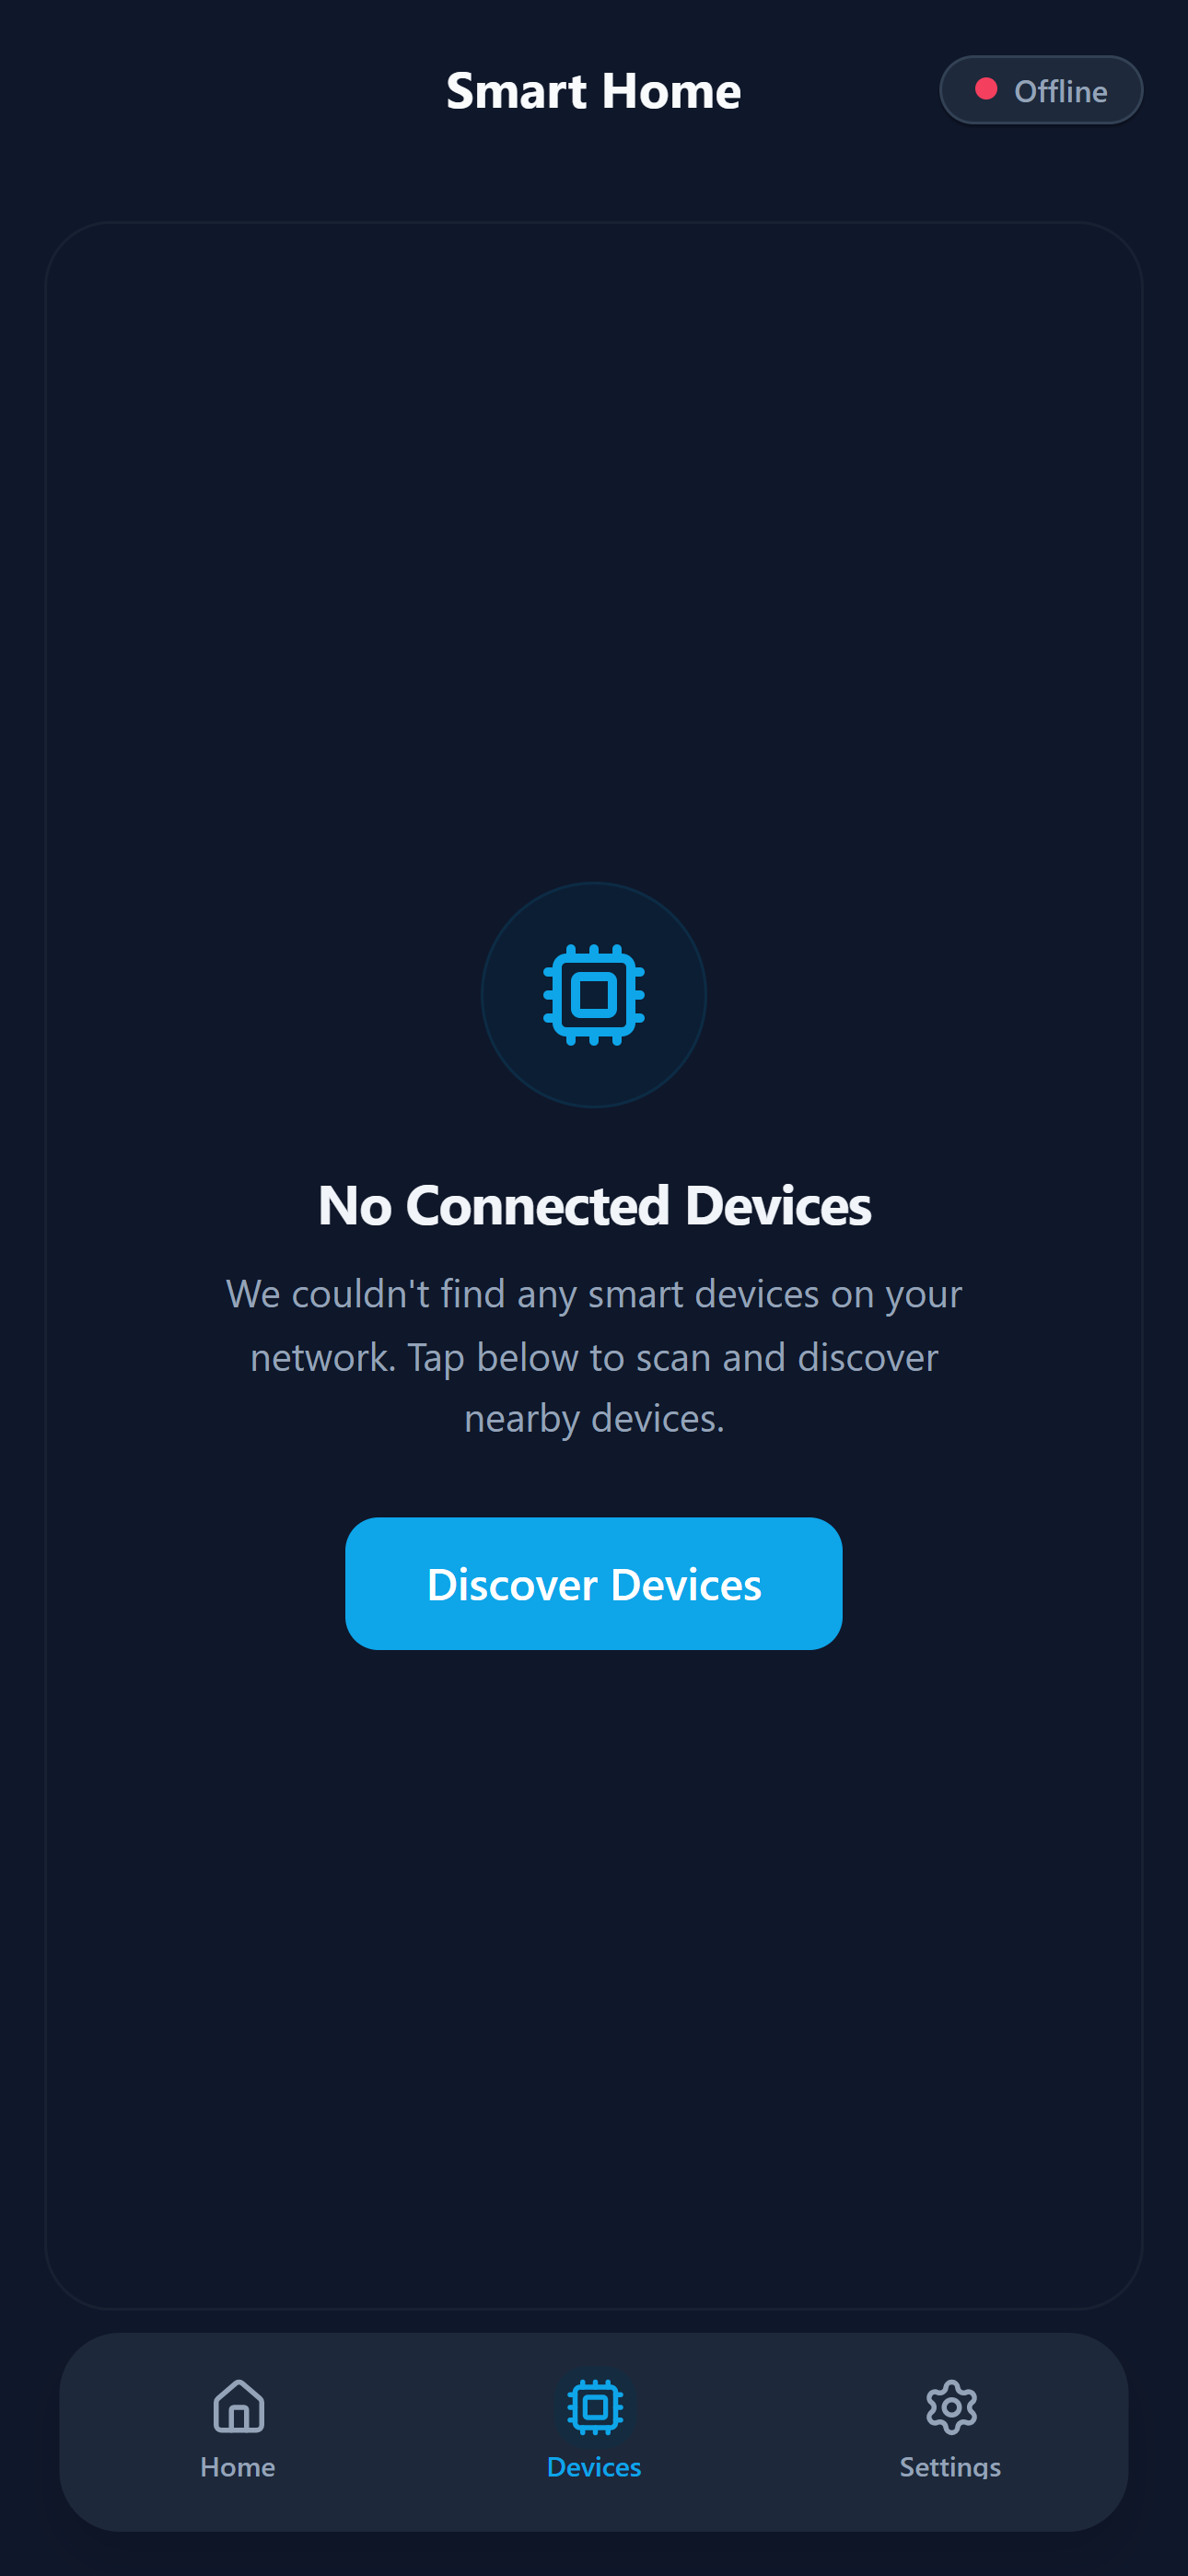
\includegraphics[width=0.45\textwidth]{figures/ch09/mobile_smarthome.png}
\caption{Smart Home control tab showing connected appliances categorized by their assigned room.}
\label{fig:mobile-smarthome}
\end{figure}

\section{Authentication \& Telegram OTP Verification}
To secure access to the wheelchair telemetry and controls, caregivers must authenticate when opening the app.

The authentication screen (\texttt{login.tsx}) handles both login and registration. If a user enters an unregistered email, the app transitions to the sign-up form, requesting their name, password, and Telegram phone number. To connect their account with the Telegram bot, the user must complete an OTP (One-Time Password) verification flow:
\begin{itemize}
    \item The app sends the user's phone number to the backend's Telegram session manager.
    \item The backend bot requests a connection code from Telegram's servers.
    \item The user receives a login code via their official Telegram app, which they enter on the mobile app's verification screen.
    \item Once verified, the backend creates a persistent Telegram session string for that user, enabling automated alert notifications.
\end{itemize}

\begin{figure}[H]
\centering
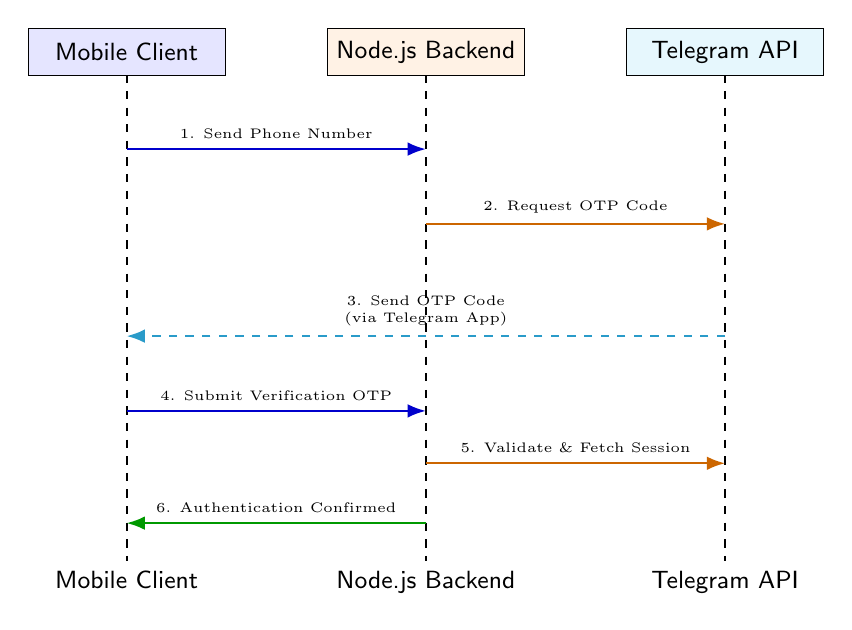
\begin{tikzpicture}[
    font=\sffamily\small,
    scale=0.95
]
    % Lifelines
    \draw[thick, dashed] (0,0) -- (0,-6.5) node[below] {Mobile Client};
    \draw[thick, dashed] (4,0) -- (4,-6.5) node[below] {Node.js Backend};
    \draw[thick, dashed] (8,0) -- (8,-6.5) node[below] {Telegram API};

    % Lifeline Headers
    \node[draw, rectangle, fill=blue!10, minimum width=2.5cm, minimum height=0.6cm] at (0,0.3) {Mobile Client};
    \node[draw, rectangle, fill=orange!10, minimum width=2.5cm, minimum height=0.6cm] at (4,0.3) {Node.js Backend};
    \node[draw, rectangle, fill=cyan!10, minimum width=2.5cm, minimum height=0.6cm] at (8,0.3) {Telegram API};

    % Steps
    \draw[-Latex, thick, draw=blue!80!black] (0,-1) -- node[above, font=\tiny] {1. Send Phone Number} (4,-1);
    \draw[-Latex, thick, draw=orange!80!black] (4,-2) -- node[above, font=\tiny] {2. Request OTP Code} (8,-2);
    \draw[-Latex, dashed, thick, draw=cyan!80!black] (8,-3.5) -- node[above, font=\tiny, align=center] {3. Send OTP Code\\(via Telegram App)} (0,-3.5);
    \draw[-Latex, thick, draw=blue!80!black] (0,-4.5) -- node[above, font=\tiny] {4. Submit Verification OTP} (4,-4.5);
    \draw[-Latex, thick, draw=orange!80!black] (4,-5.2) -- node[above, font=\tiny] {5. Validate \& Fetch Session} (8,-5.2);
    \draw[-Latex, thick, draw=green!60!black] (4,-6) -- node[above, font=\tiny] {6. Authentication Confirmed} (0,-6);

\end{tikzpicture}
\caption{Sequence diagram illustrating the Telegram OTP authentication and persistent session handshake flow.}
\label{fig:mobile-otp-sequence}
\end{figure}

\begin{figure}[H]
\centering
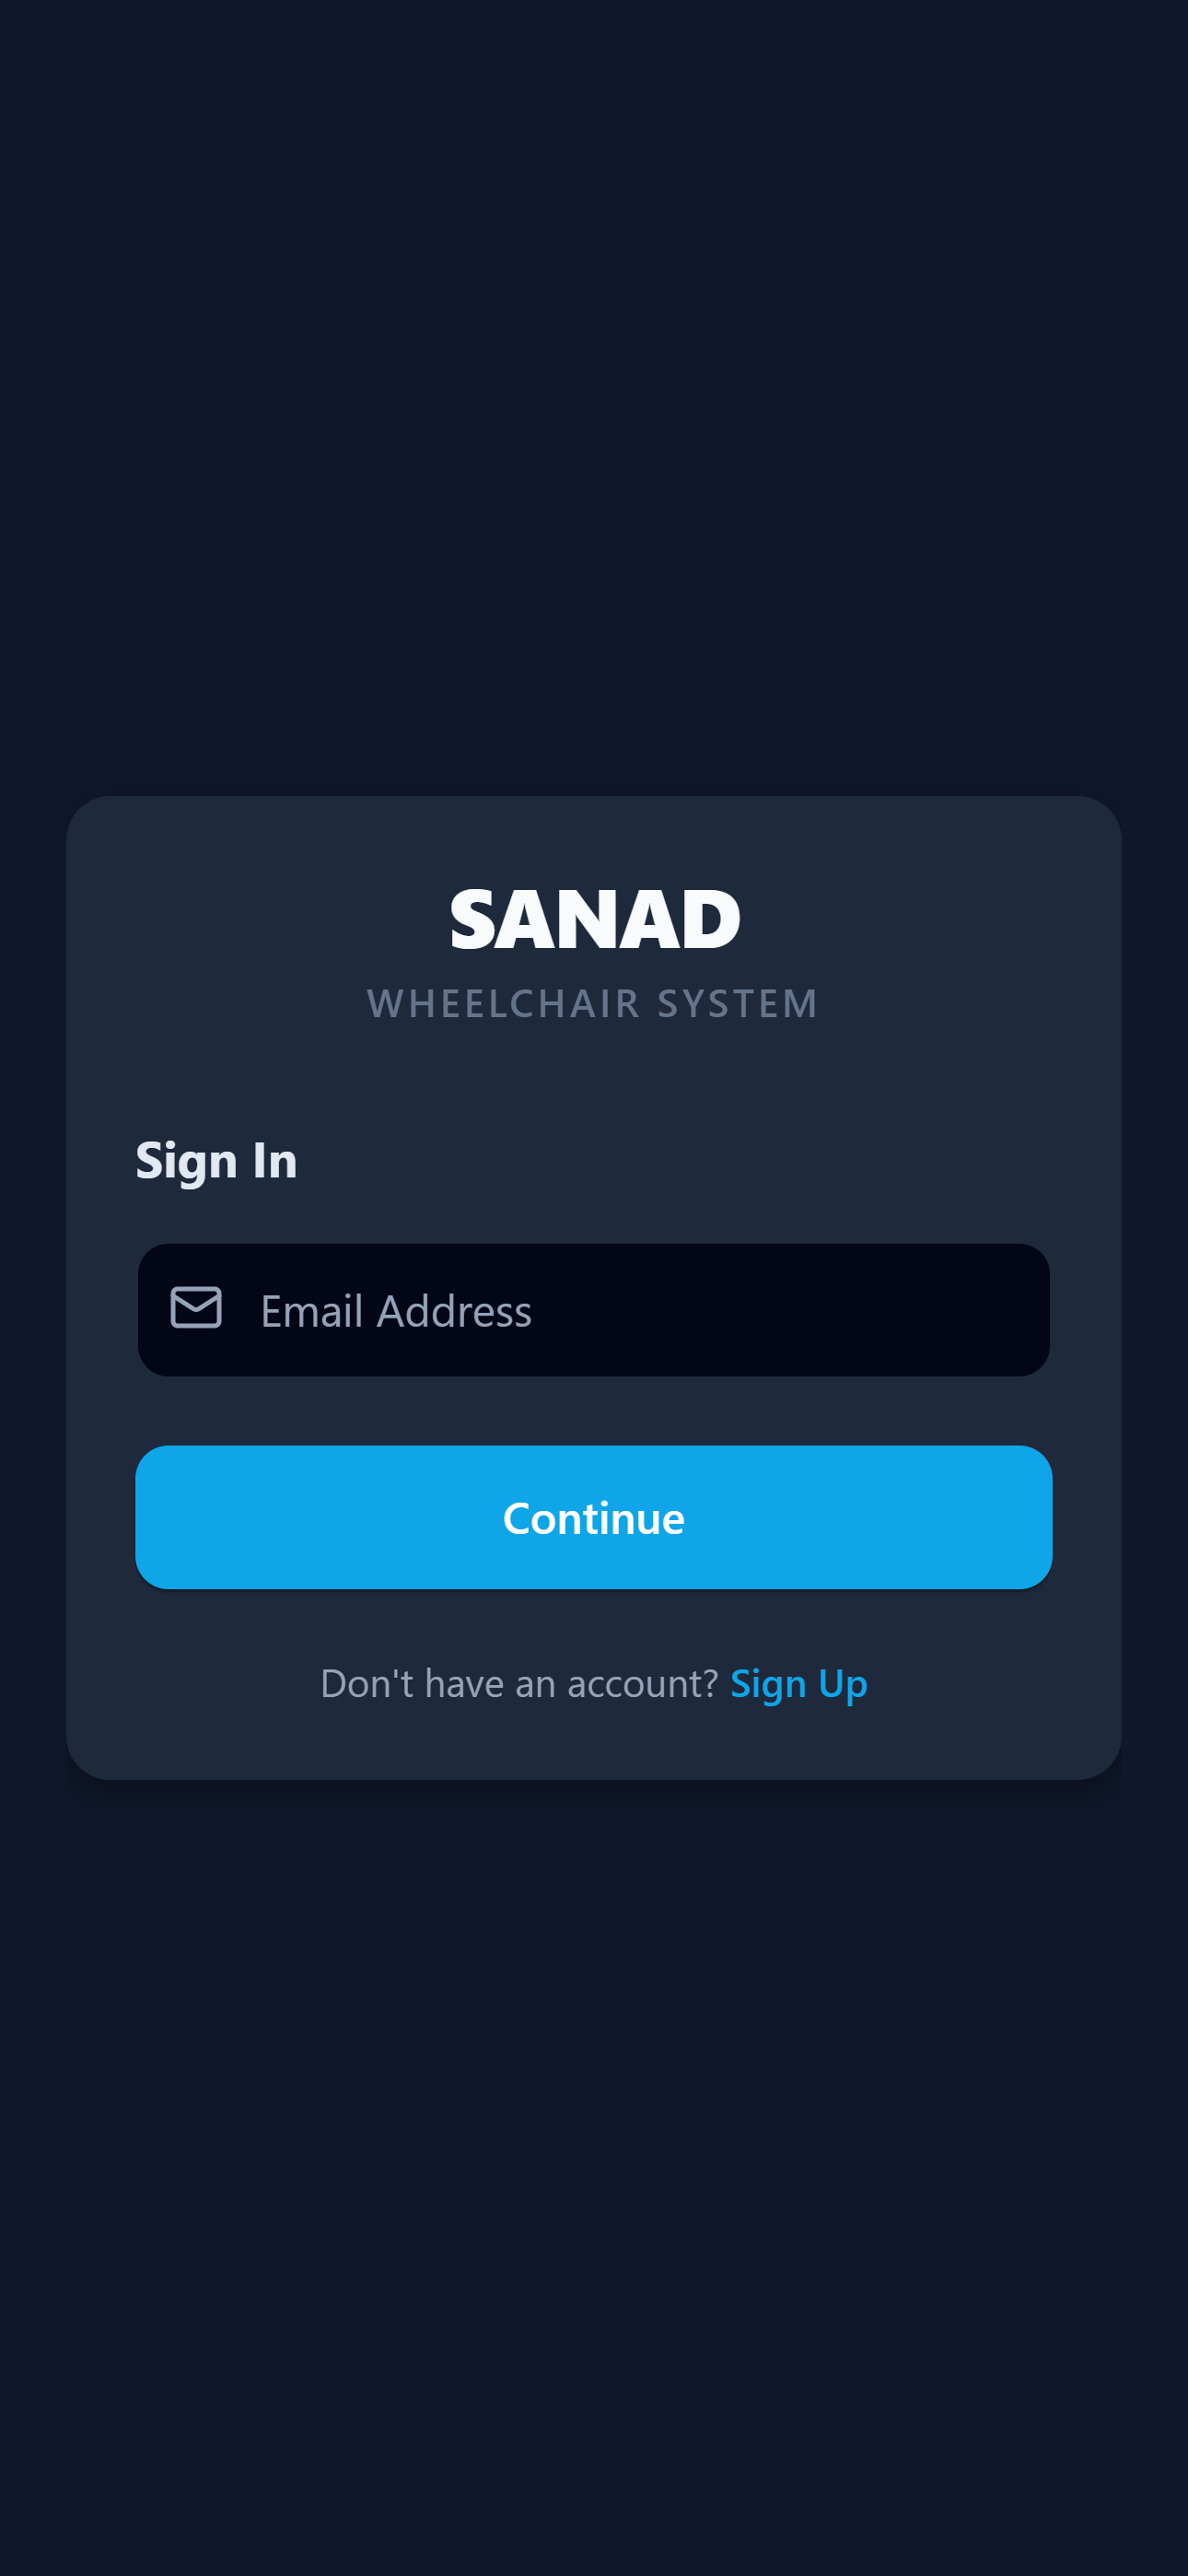
\includegraphics[width=0.48\textwidth]{figures/ch09/mobile_login.png}
\caption{Caregiver login and registration interface in the mobile application.}
\label{fig:mobile-login}
\end{figure}

\begin{figure}[H]
\centering
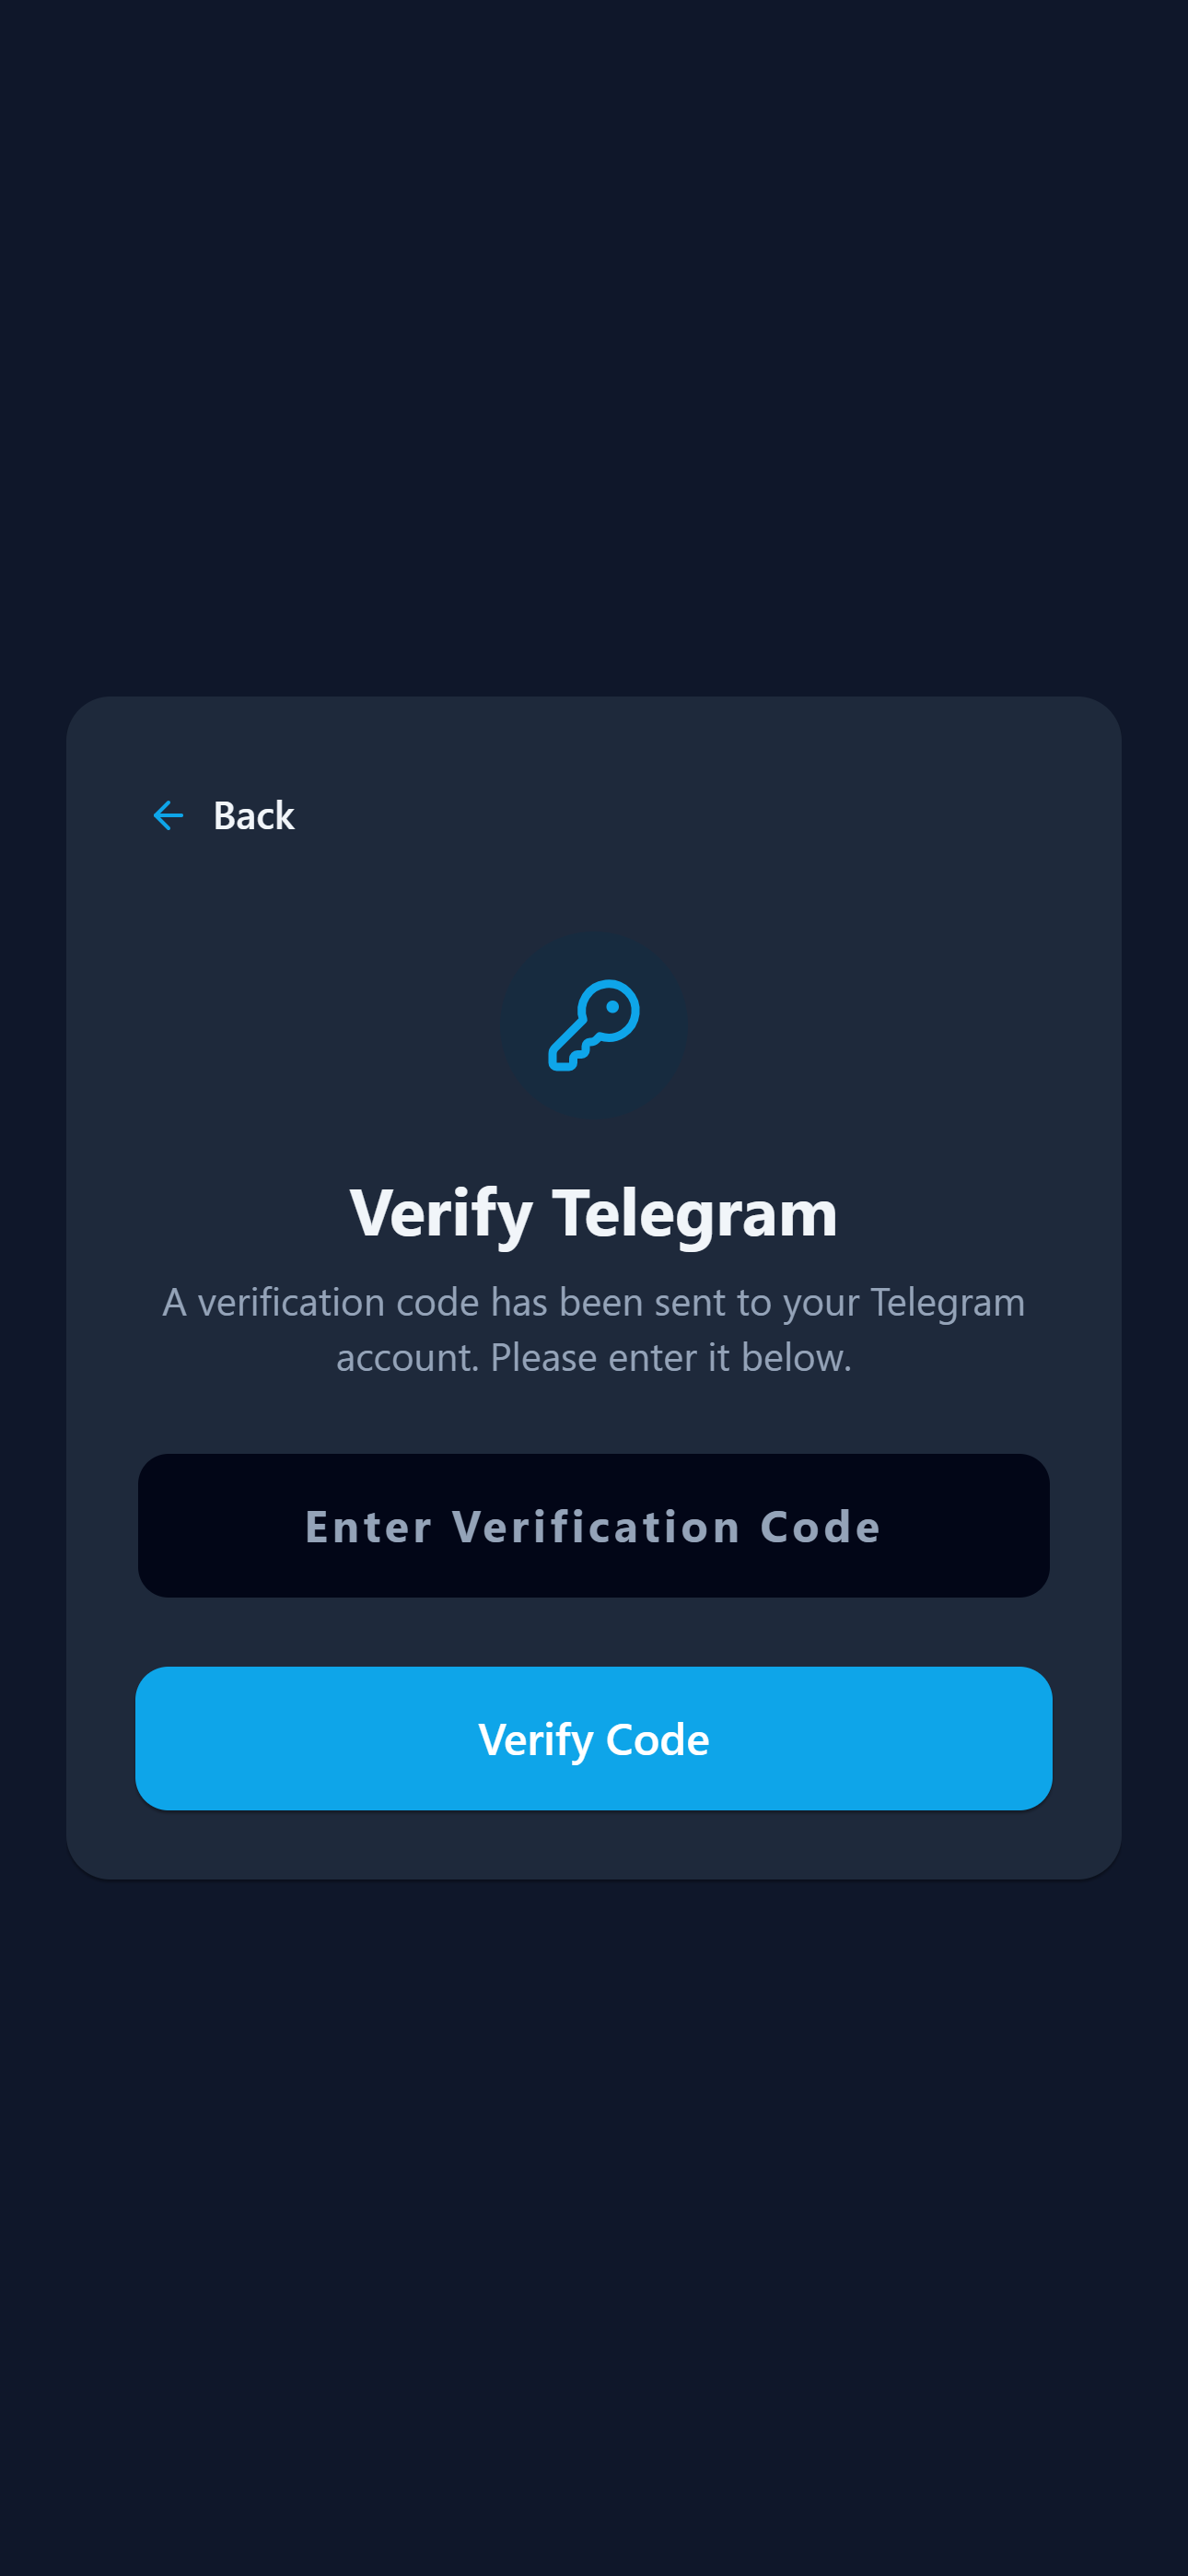
\includegraphics[width=0.48\textwidth]{figures/ch09/mobile_otp.png}
\caption{Telegram OTP Verification screen requesting the authentication code sent to the caregiver's Telegram client.}
\label{fig:mobile-otp}
\end{figure}

\section{Accessibility \& Haptic Feedback}
The mobile app is designed to be accessible to a wide range of users, using physical haptic feedback and accessibility tags to improve usability.

\subsection{Haptic Verification}
To reassure users that their actions and alert thresholds have been updated successfully, the app uses device vibration patterns powered by \texttt{expo-haptics} when saves occur. In addition, the device triggers vibration alerts when emergency alerts are dispatched, helping to draw attention to critical vitals breaches.

\subsection{Accessibility Elements}
The UI is optimized for screen readers (like VoiceOver on iOS and TalkBack on Android). Buttons and interactive elements use semantic labels (\texttt{accessibilityLabel}) and state markers (\texttt{accessibilityState}), and touch targets are sized to at least $48 \times 48$ density-independent pixels to ensure they are easy to select.

\begin{figure}[H]
\centering
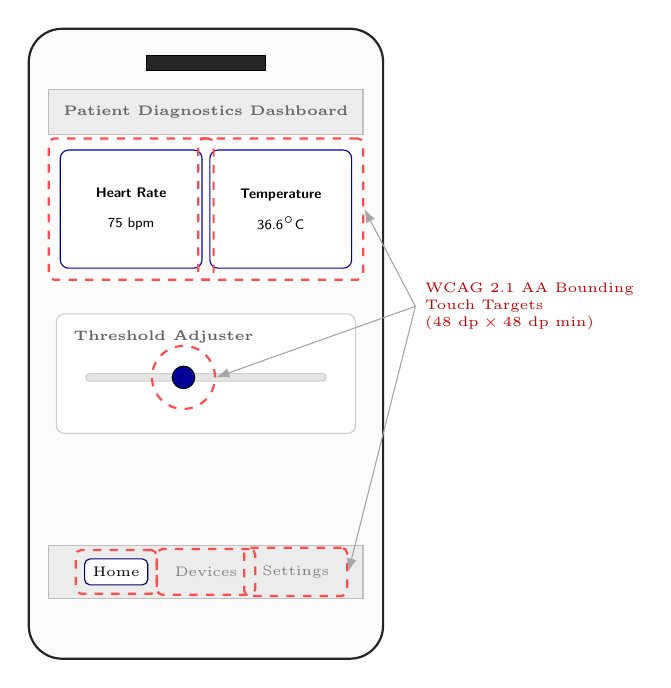
\begin{tikzpicture}[
    font=\sffamily\small,
    scale=0.95,
    phone/.style={draw=black!85, thick, fill=gray!3, rounded corners=12pt, minimum width=4.5cm, minimum height=8.0cm},
    card/.style={draw=blue!70!black, fill=white, rounded corners=3pt, minimum width=1.8cm, minimum height=1.5cm, align=center},
    targetZone/.style={draw=red!70, dashed, thick, rounded corners=2pt},
    arrow/.style={-Latex, thin, draw=gray!70}
]

    % Phone Body
    \node[phone] (screen) {};
    
    % Speaker/Camera Notch
    \draw[fill=black!85] (-0.8,3.85) rectangle (0.8,3.65);

    % Screen Header
    \draw[draw=gray!50, fill=gray!15] (-2.1,3.4) rectangle (2.1,2.8);
    \node[font=\tiny\bfseries, text=gray!80!black] at (0,3.1) {Patient Diagnostics Dashboard};
    
    % Card Row 1: Vitals Grid
    \node[card] (hrCard) at (-1.0, 1.8) {\tiny\bfseries Heart Rate\\\tiny 75 bpm};
    \node[card] (tempCard) at (1.0, 1.8) {\tiny\bfseries Temperature\\\tiny 36.6$^\circ$C};
    
    % Dash Touch target zones overlaying cards
    \node[targetZone, fit=(hrCard), inner sep=4pt] (hrTarget) {};
    \node[targetZone, fit=(tempCard), inner sep=4pt] (tempTarget) {};

    % Slider Control Section
    \draw[draw=gray!40, fill=white, rounded corners=3pt] (-2.0, 0.4) rectangle (2.0, -1.2);
    \node[anchor=north west, font=\tiny\bfseries, text=gray!80!black] at (-1.9,0.3) {Threshold Adjuster};
    
    % Slider bar
    \draw[draw=gray!40, fill=gray!20, rounded corners=1pt] (-1.6, -0.4) rectangle (1.6, -0.5);
    \draw[fill=blue!60!black] (-0.3, -0.45) circle (0.15cm);
    
    % Slider Thumb touch target zone
    \node[targetZone, circle, minimum size=0.8cm] (thumbTarget) at (-0.3, -0.45) {};

    % Bottom Navigation Bar
    \draw[draw=gray!50, fill=gray!15] (-2.1,-3.4) rectangle (2.1,-2.7);
    \node[draw=blue!40!black, fill=white, rounded corners=2pt, font=\tiny, inner sep=3pt] (tabHome) at (-1.2, -3.05) {Home};
    \node[font=\tiny, text=gray] (tabSmart) at (0, -3.05) {Devices};
    \node[font=\tiny, text=gray] (tabSet) at (1.2, -3.05) {Settings};
    
    \node[targetZone, fit=(tabHome), inner sep=3pt] (t1) {};
    \node[targetZone, fit=(tabSmart), inner sep=3pt] (t2) {};
    \node[targetZone, fit=(tabSet), inner sep=3pt] (t3) {};

    % Annotations
    \node[anchor=west, font=\tiny, text=red!80!black, align=left] (targetLabel) at (2.8, 0.5) {WCAG 2.1 AA Bounding\\Touch Targets\\($48\text{ dp} \times 48\text{ dp}$ min)};
    
    \draw[arrow] (targetLabel.west) -- (tempTarget.east);
    \draw[arrow] (targetLabel.west) -- (thumbTarget.east);
    \draw[arrow] (targetLabel.west) -- (t3.east);

\end{tikzpicture}
\caption{UX layout wireframe showing dashboard card structure, Flexbox spacing, and accessibility touch target zones (minimum $48 \times 48\text{ dp}$ bounds) for the mobile app interface.}
\label{fig:mobile-wireframe}
\end{figure}

\section{System Diagnostics}
The settings panel (\texttt{settings.tsx}) displays system diagnostic information to help caregivers monitor the wheelchair's status.

When connected to the server, the app subscribes to status topics like battery state and diagnostics. It parses these messages to display:
\begin{itemize}
    \item \textbf{Battery Level}: Extracted from the battery state message percentage.
    \item \textbf{Speed Limit}: The current speed limit setting (0--100\%).
    \item \textbf{System Temperature}: The CPU temperature of the onboard computer.
    \item \textbf{Uptime}: The elapsed time since the system was powered on.
\end{itemize}
This panel also allows caregivers to update the server's API URL when connecting to different local networks.

\begin{figure}[H]
\centering
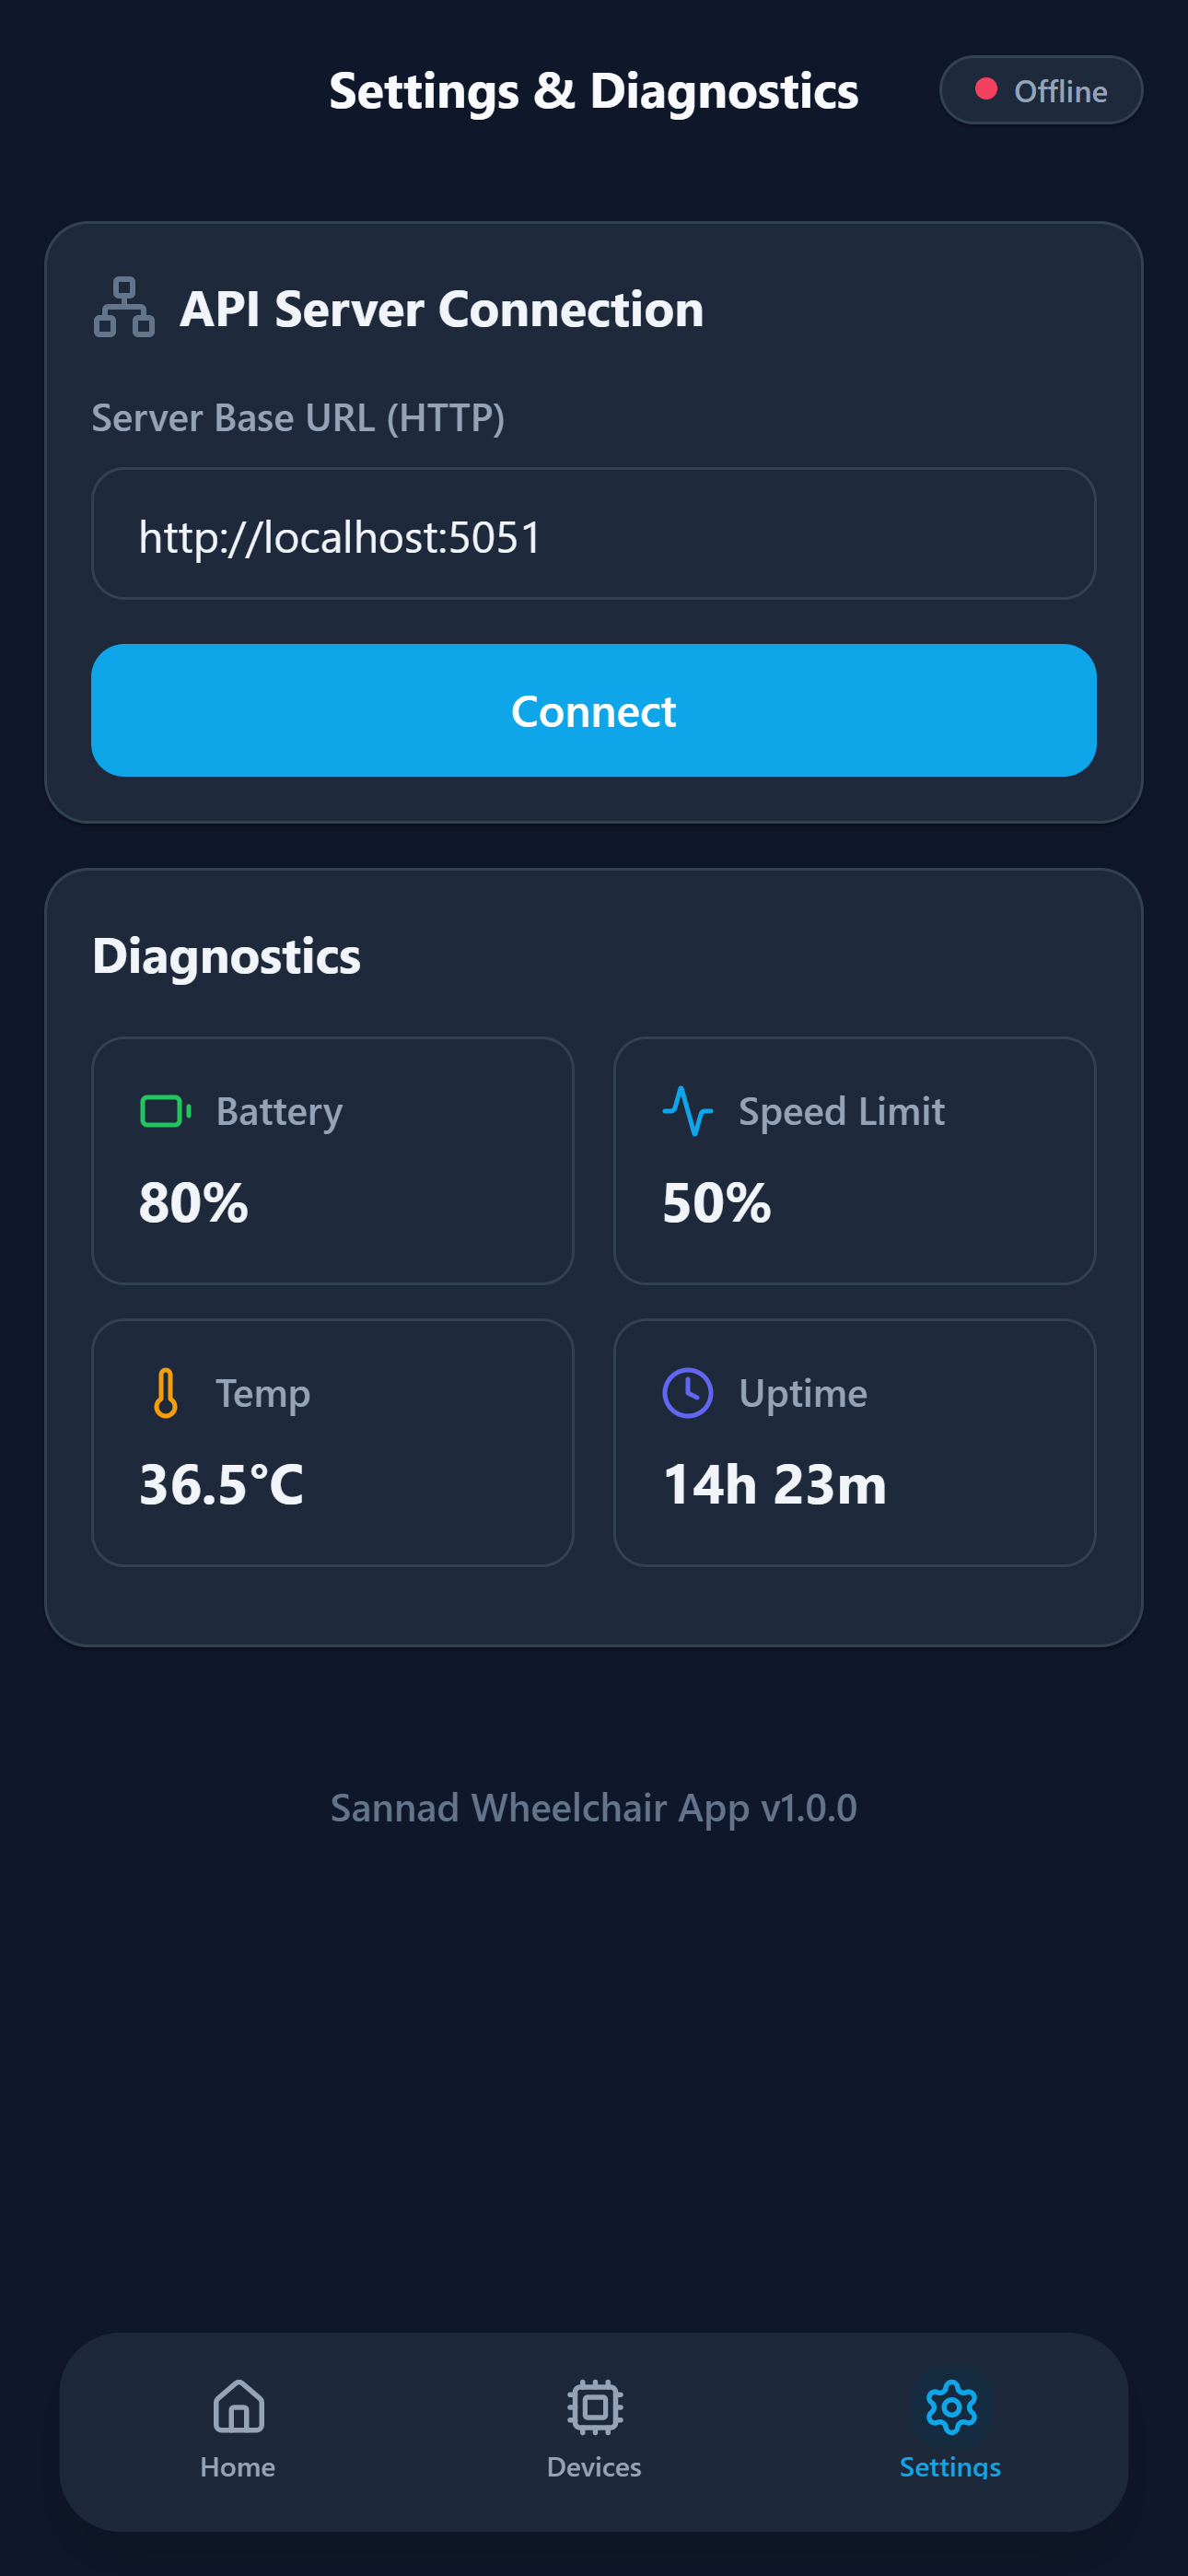
\includegraphics[width=0.45\textwidth]{figures/ch09/mobile_settings.png}
\caption{Settings and Diagnostics view showing server configuration inputs and active wheelchair diagnostic readings.}
\label{fig:mobile-settings}
\end{figure}

\section{Summary and Transition}
This chapter has detailed the design of the React Native mobile app, highlighting caregiver biometrics telemetry and remote system diagnostic capabilities. The next chapter, Chapter 10 (Hardware \& Implementation), focuses on the physical integration, custom circuit layouts, motor control loops, and power configurations of the wheelchair.


\chapterseparator{Chapter 10}
% NOTE: requires \usepackage{subcaption} in the preamble (in addition to graphicx, tikz, tabularx already used).
% NOTE: For figure/table numbers to be CLICKABLE (jump to the figure/table when clicked),
% the main document preamble must load \usepackage{hyperref} (ideally last, after other packages).
% With hyperref loaded, every \ref{...} / \autoref{...} below automatically becomes a clickable link.

\setcounter{chapter}{10}
\chapter*{Chapter (10): Hardware \& Implementation}
\addcontentsline{toc}{chapter}{Chapter (10): Hardware \& Implementation}
\setcounter{section}{0}

\section{Chapter Preview}
This chapter details the physical integration and mechanical/electrical design of the Sanad prototype. It explains chassis modifications, drivetrain design calculations, PID motor control tuning, power distribution circuits, and concludes with a detailed Bill of Materials (BOM) cost breakdown.

\section{Wheelchair Modifications Over the Manual Platform}
All physical build decisions, from wheelchair frame modifications to the power system, are documented in this chapter in enough detail for replication. This chapter describes the physical implementation of the Sanad smart wheelchair system, including mechanical modifications, motor control architecture, hardware interfacing, and power distribution. The system integrates multiple sensing and interaction modalities while maintaining the structural integrity and safety of the original wheelchair platform.

The original wheelchair platform is a foldable electric wheelchair equipped with two 24\,V, 250\,W brushed DC motors and a 24\,V, 12\,Ah lead-acid battery system capable of carrying up to 120\,kg. This section describes how the base platform was modified to host the sensors, compute units, and assistive modules required for autonomous navigation and human-robot interaction. Figure~\ref{fig:wheelchair-base-views} shows the unmodified base platform before any modifications were carried out.

\begin{figure}[H]
    \centering
    \begin{subfigure}[t]{0.48\textwidth}
        \centering
        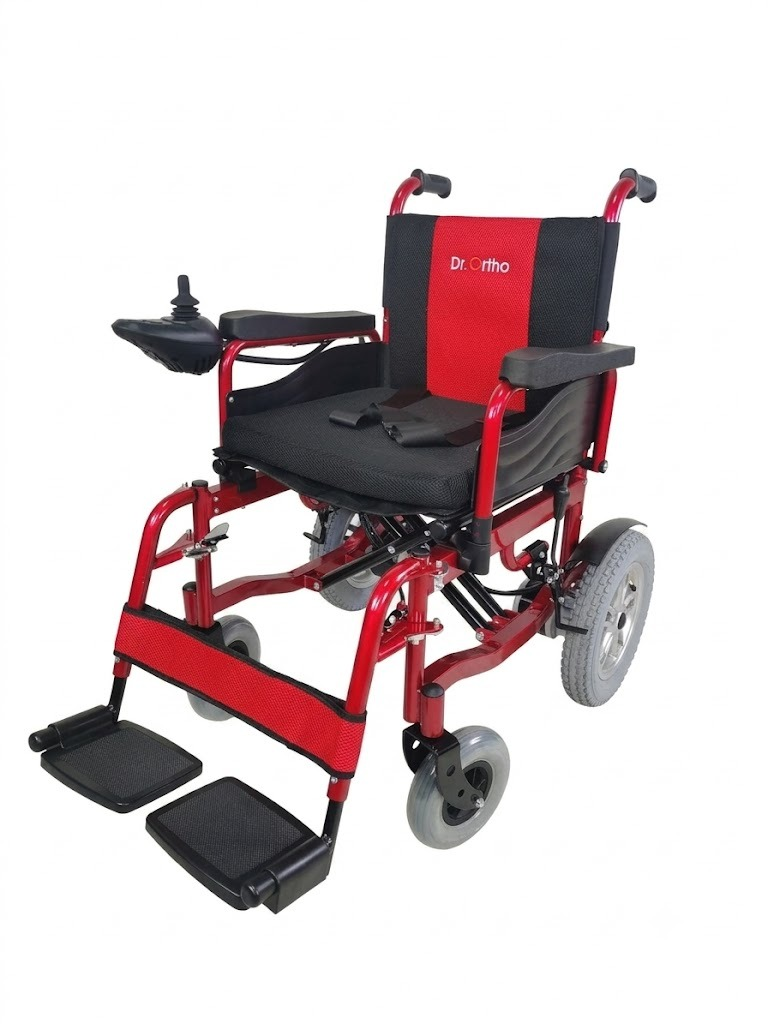
\includegraphics[height=0.32\textheight,keepaspectratio]{figures/ch10/wheelchair-platform}
        \caption{Front view.}
        \label{fig:wheelchair-platform}
    \end{subfigure}\hfill
    \begin{subfigure}[t]{0.48\textwidth}
        \centering
        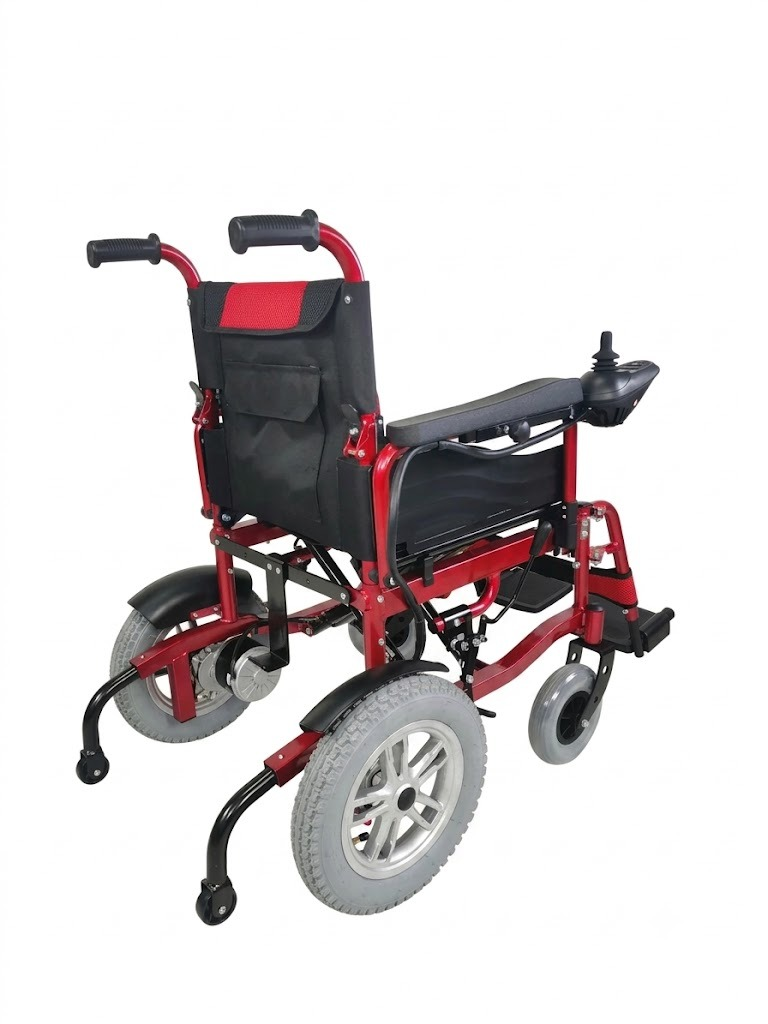
\includegraphics[height=0.32\textheight,keepaspectratio]{figures/ch10/structural-overview}
        \caption{Rear view.}
        \label{fig:structural-overview}
    \end{subfigure}
    \caption{Base wheelchair, real photographs: (a) front view, (b) rear view.}
    \label{fig:wheelchair-base-views}
\end{figure}

\subsection{Base Platform and Mechanical Integration}

To support autonomous navigation, obstacle avoidance, and assistive interaction, a set of sensors and actuators were added to the base wheelchair frame using custom 3D-printed and welded mounts. Each subsystem was positioned to maximize sensor coverage while keeping the wheelchair's footprint, weight distribution, and foldability largely unchanged.

Figure~\ref{fig:structural-overview-diagram} presents a structural overview of all hardware modifications and illustrates how each subsystem interfaces with the Raspberry Pi~5, which serves as the central computing unit of the wheelchair. The subsections that follow walk through how each of these subsystems was physically integrated into the platform, grouped by function: navigation sensing, drivetrain instrumentation, and assistive modules.

\begin{figure}[H]
    \centering
    % Replace the file name with your own image
    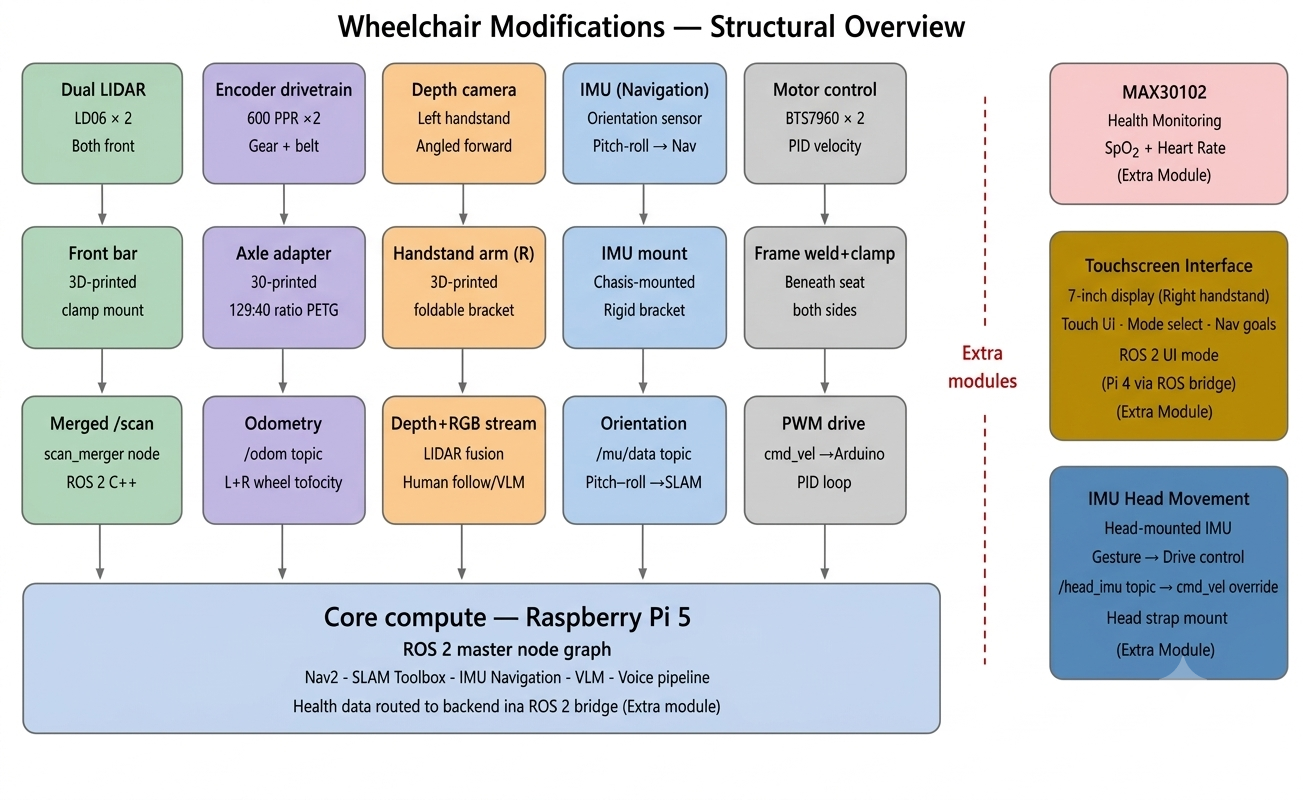
\includegraphics[width=\textwidth]{figures/ch10/structural-overview-diagram}
    \caption{Structural overview of the wheelchair modifications and the data flow .}
    \label{fig:structural-overview-diagram}
\end{figure}

\subsection{Navigation Sensor Integration}

The navigation stack relies on three sensing modalities -- LiDAR, an RGB-D camera, and an IMU -- each mounted so as to give the system consistent, interference-free coverage of the environment ahead of and around the wheelchair.

\subsection*{Dual LiDAR Mount}
Two LD06 LiDAR sensors were mounted at the front of the wheelchair using a custom 3D-printed front bar.
\begin{itemize}
\item It provides the environmental information required for mapping and localization.
\item It enables accurate obstacle detection and safe navigation.
\item It improves the reliability of autonomous navigation.
\end{itemize}

% TODO (pending clarification): user asked to check whether this figure has a lot of
% empty space below it, and if so, to merge the LiDAR holder figure's (a) and (b)
% subfigures into it instead of keeping them as a separate two-part figure below.
% Not applied yet -- waiting to confirm this is the intended figure pair.
Figure~\ref{fig:lidar-mount} shows the LD06 LiDAR sensor mounted at the front of the wheelchair using the custom 3D-printed bar described above.

\begin{figure}[H]
    \centering
    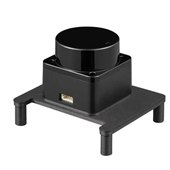
\includegraphics[height=0.22\textheight,keepaspectratio]{figures/ch10/lidar-mount}
    \caption{LD06 LiDAR sensor mount at the front of the wheelchair.}
    \label{fig:lidar-mount}
\end{figure}

Figure~\ref{fig:lidar-holder} shows the CAD model of the LiDAR holder alongside the corresponding fabricated 3D-printed part used to secure each sensor.

\begin{figure}[H]
    \centering
    \begin{subfigure}[t]{0.48\textwidth}
        \centering
        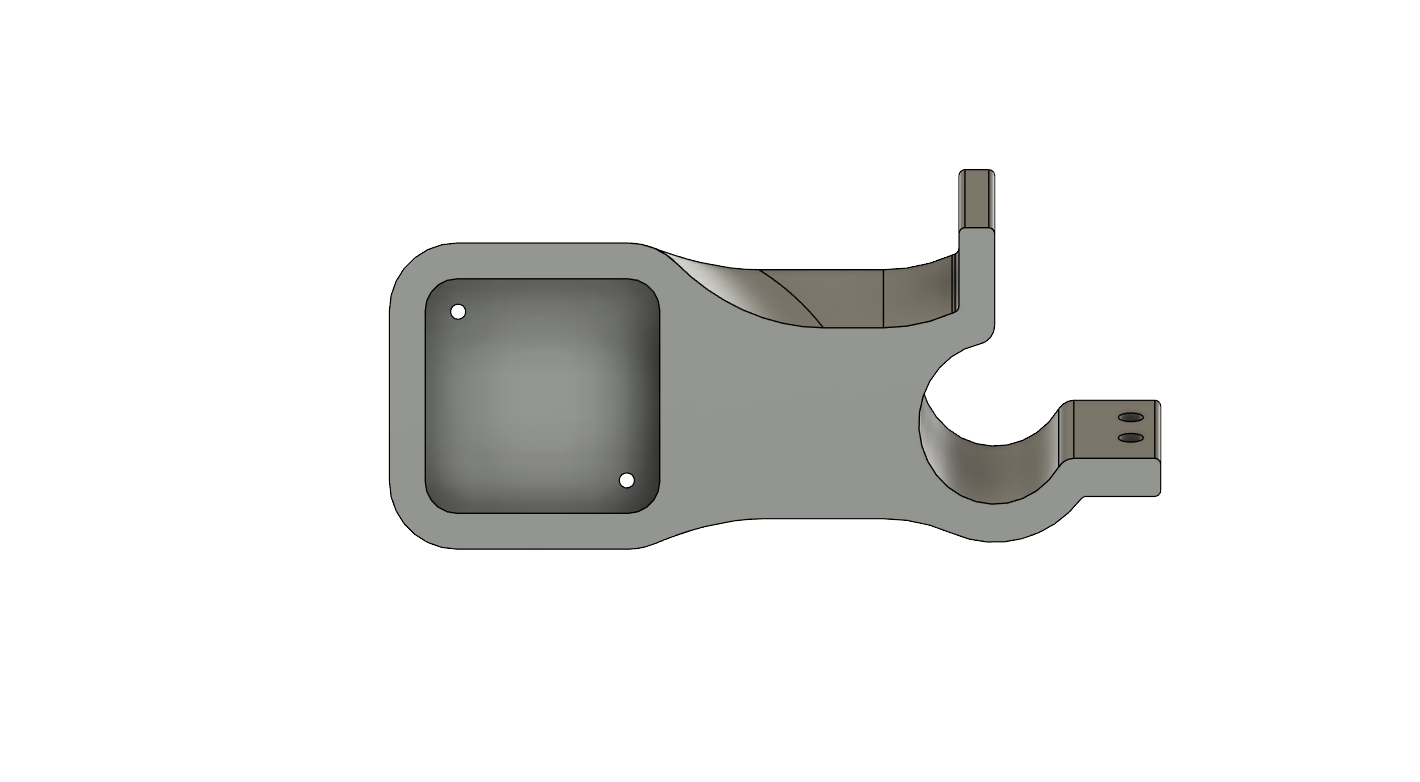
\includegraphics[height=0.22\textheight,keepaspectratio]{figures/ch10/lidar-holder-cad}
        \caption{3D CAD model (Autodesk Fusion).}
        \label{fig:lidar-holder-cad}
    \end{subfigure}\hfill
    \begin{subfigure}[t]{0.48\textwidth}
        \centering
        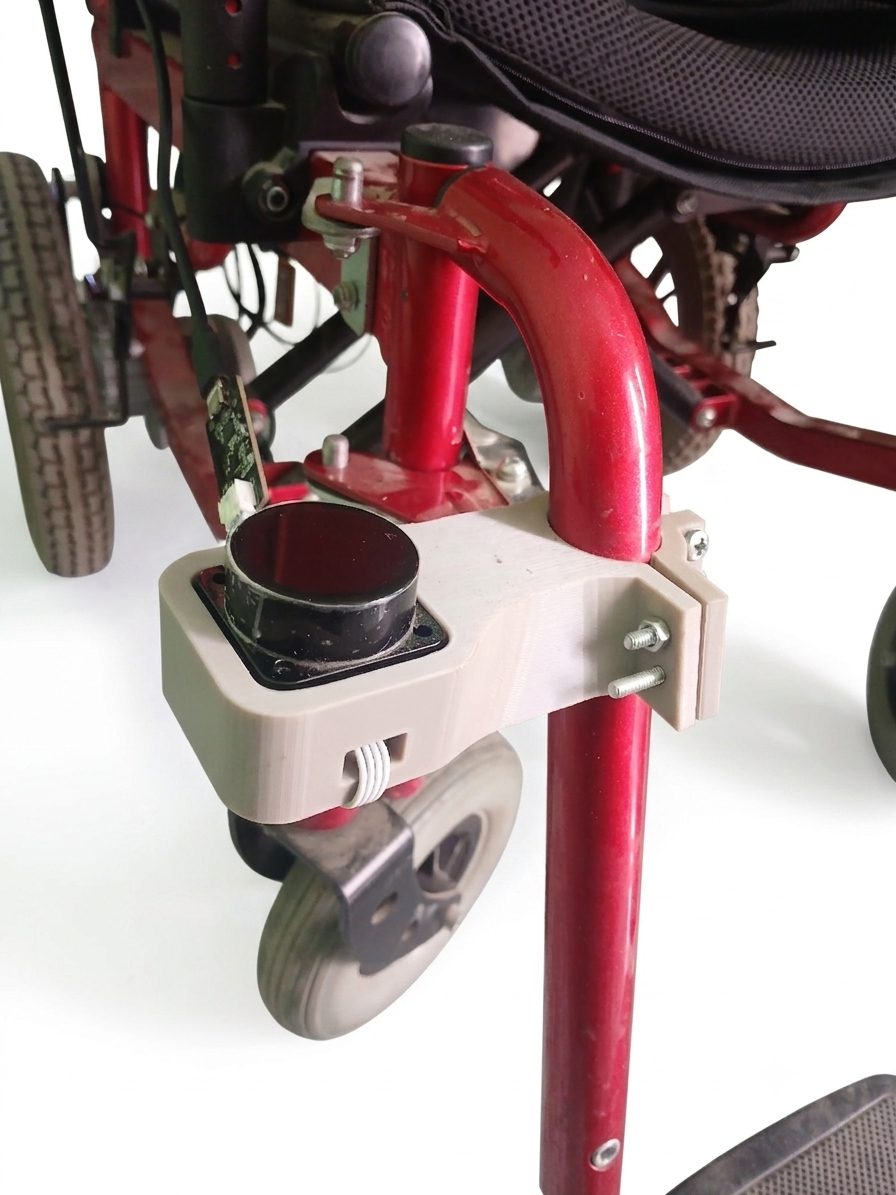
\includegraphics[height=0.22\textheight,keepaspectratio]{figures/ch10/lidar-holder-real}
        \caption{3D-printed part after fabrication.}
        \label{fig:lidar-holder-real}
    \end{subfigure}
    \caption{LiDAR holder: (a) 3D CAD model, (b) fabricated 3D-printed part.}
    \label{fig:lidar-holder}
\end{figure}

The front dual-LiDAR bar shown in Figure~\ref{fig:lidar-holder} fixes both LD06 units at a fixed relative angle, guaranteeing the combined field of view assumed in the SLAM configuration.

\subsection*{Depth Camera Mount}
The RGB-D camera was installed on the left armrest using an angled bracket, oriented forward and slightly downward so that it can track people and obstacles directly ahead of the wheelchair.
\begin{itemize}
\item Human following.
\item Object detection.
\item Environment perception.
\end{itemize}

Figure~\ref{fig:depth-camera-mount} shows the RGB-D camera mounted on the left armrest in this forward-and-downward-facing orientation.

\begin{figure}[H]
    \centering
    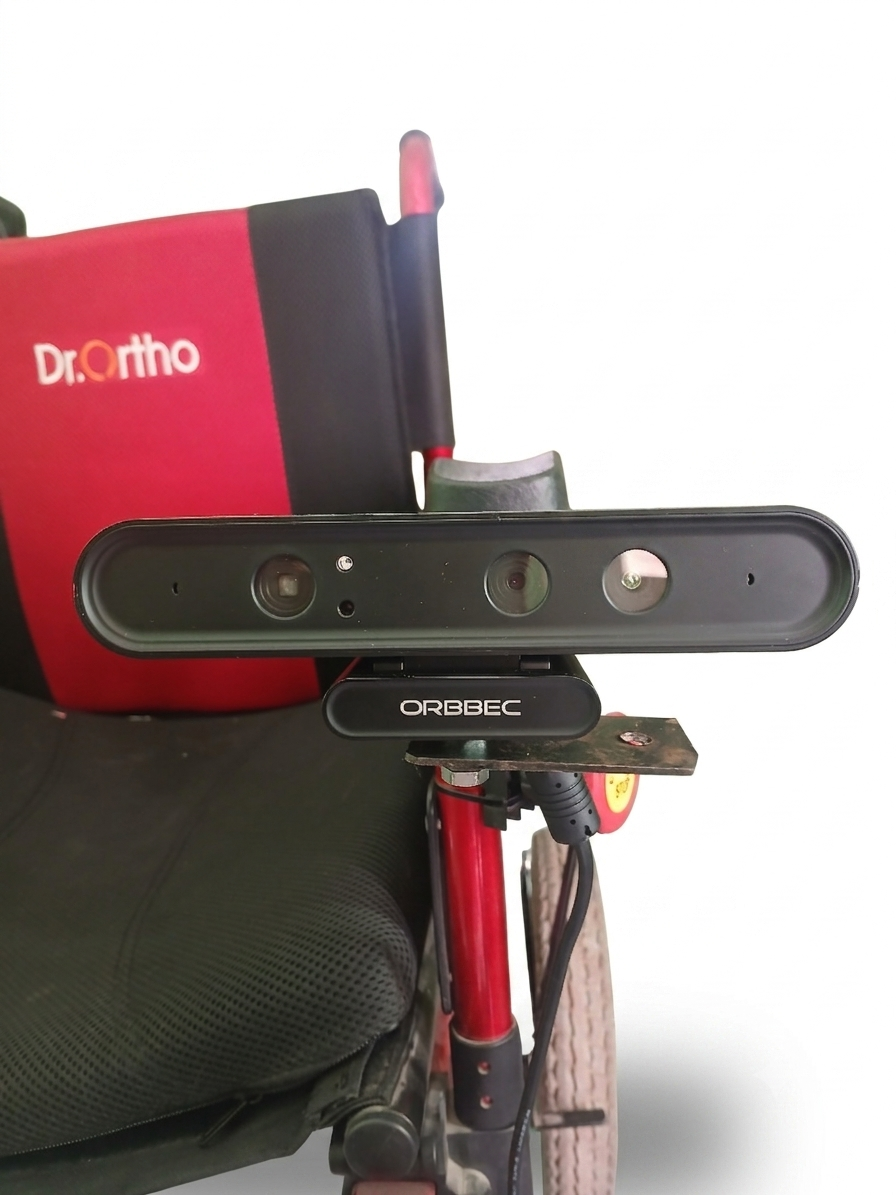
\includegraphics[height=0.18\textheight,keepaspectratio]{figures/ch10/depth-camera-mount}
    \caption{RGB-D camera mount on the left armrest.}
    \label{fig:depth-camera-mount}
\end{figure}

\subsection*{Navigation IMU Mount}
An inertial measurement unit (IMU) was rigidly mounted to the chassis beneath the seat to provide continuous orientation data for the navigation stack. Working alongside the LiDAR and depth camera, this sensor improves the robustness of SLAM-based localization, particularly when the wheelchair encounters uneven surfaces or slight inclines.
\begin{itemize}
\item Measures the wheelchair orientation.
\item Improves localization accuracy and overall navigation performance.
\end{itemize}

Figure~\ref{fig:imu-mount} shows the IMU rigidly mounted beneath the wheelchair seat.

\begin{figure}[H]
    \centering
    \tikz[baseline=(img.base)] \node[inner sep=0pt,fill=white] (img) {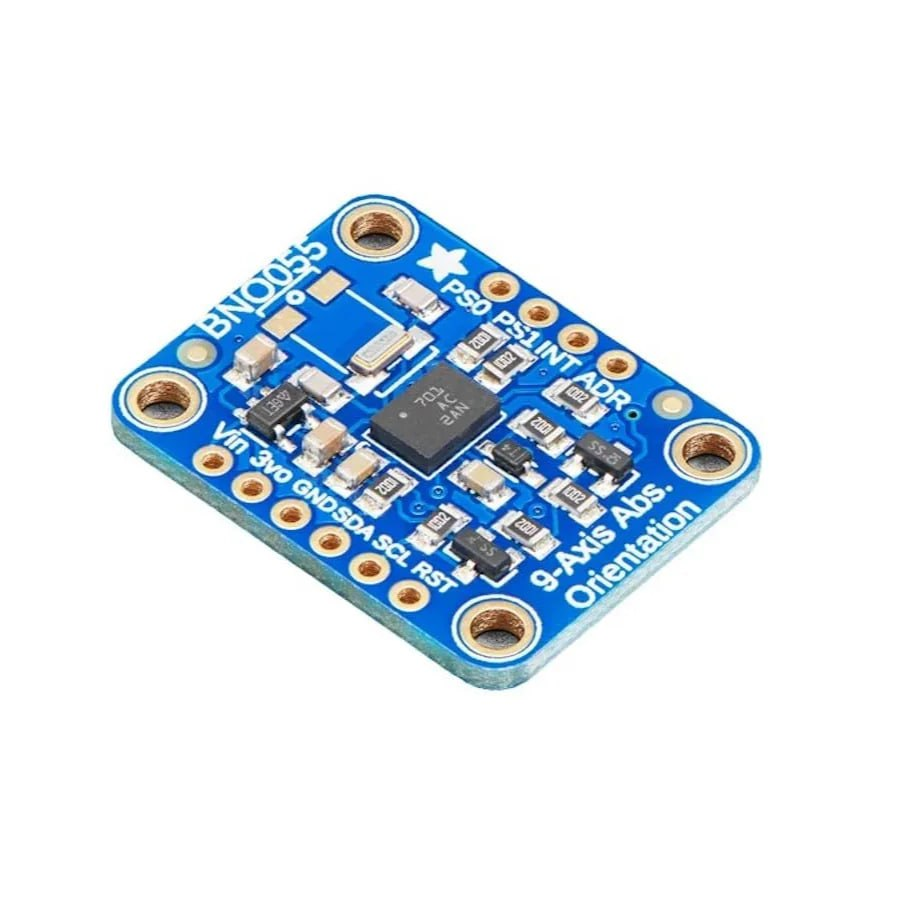
\includegraphics[height=0.18\textheight,keepaspectratio]{figures/ch10/imu-mount}};
    \caption{IMU mounted beneath the wheelchair seat.}
    \label{fig:imu-mount}
\end{figure}

\subsection{Drive System Integration}

Closed-loop control of the drivetrain requires accurate wheel-speed feedback and current-capable motor drivers, both integrated close to the wheels to keep cabling short and signal quality high.

\subsection*{Encoder Installation}
To close the velocity control loop and support accurate odometry, an incremental rotary encoder was mechanically coupled to each drive wheel through a custom GT2 belt-and-pulley transmission. The encoder output is read by the Arduino Nano and used both for real-time speed control and for generating odometry data for the ROS 2 navigation stack.
\begin{itemize}
\item Measure wheel speed accurately.
\item Provide feedback for the PID speed controller.
\item Generate odometry information for localization and navigation.
\item Maintain stable motor speed under varying loads and terrain conditions.
\item Improve motion accuracy during autonomous navigation.
\end{itemize}

Additional encoder-based odometry is also used to detect slip and improve the stability of closed-loop velocity control across variable loads, ensuring the wheelchair follows commanded paths with minimal drift. Figure~\ref{fig:encoder-drivetrain} shows the incremental rotary encoder module used for this purpose.

% TODO (pending clarification): same possible candidate as the LiDAR figures above --
% if this is the figure with a lot of empty space below it, the encoder holder
% figure's (a) and (b) subfigures could be merged into it instead. Not applied yet.
\begin{figure}[H]
    \centering
    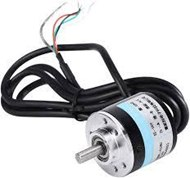
\includegraphics[height=0.18\textheight,keepaspectratio]{figures/ch10/encoder-drivetrain}
    \caption{Incremental rotary encoder module used for wheel speed measurement.}
    \label{fig:encoder-drivetrain}
\end{figure}

\begin{figure}[H]
    \centering
    \begin{subfigure}[t]{0.48\textwidth}
        \centering
        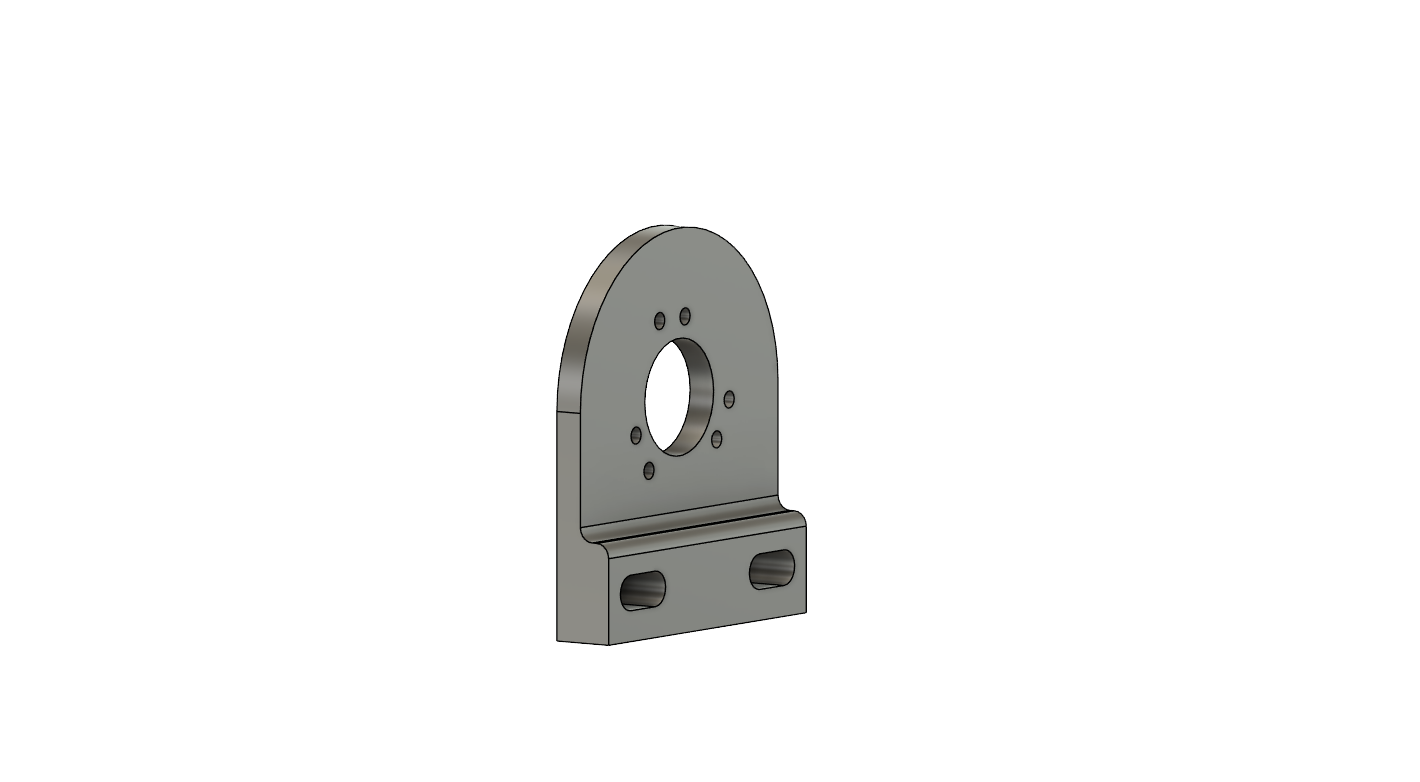
\includegraphics[height=0.22\textheight,keepaspectratio]{figures/ch10/encoder-holder-cad}
        \caption{3D CAD model (Autodesk Fusion).}
        \label{fig:encoder-holder-cad}
    \end{subfigure}\hfill
    \begin{subfigure}[t]{0.48\textwidth}
        \centering
        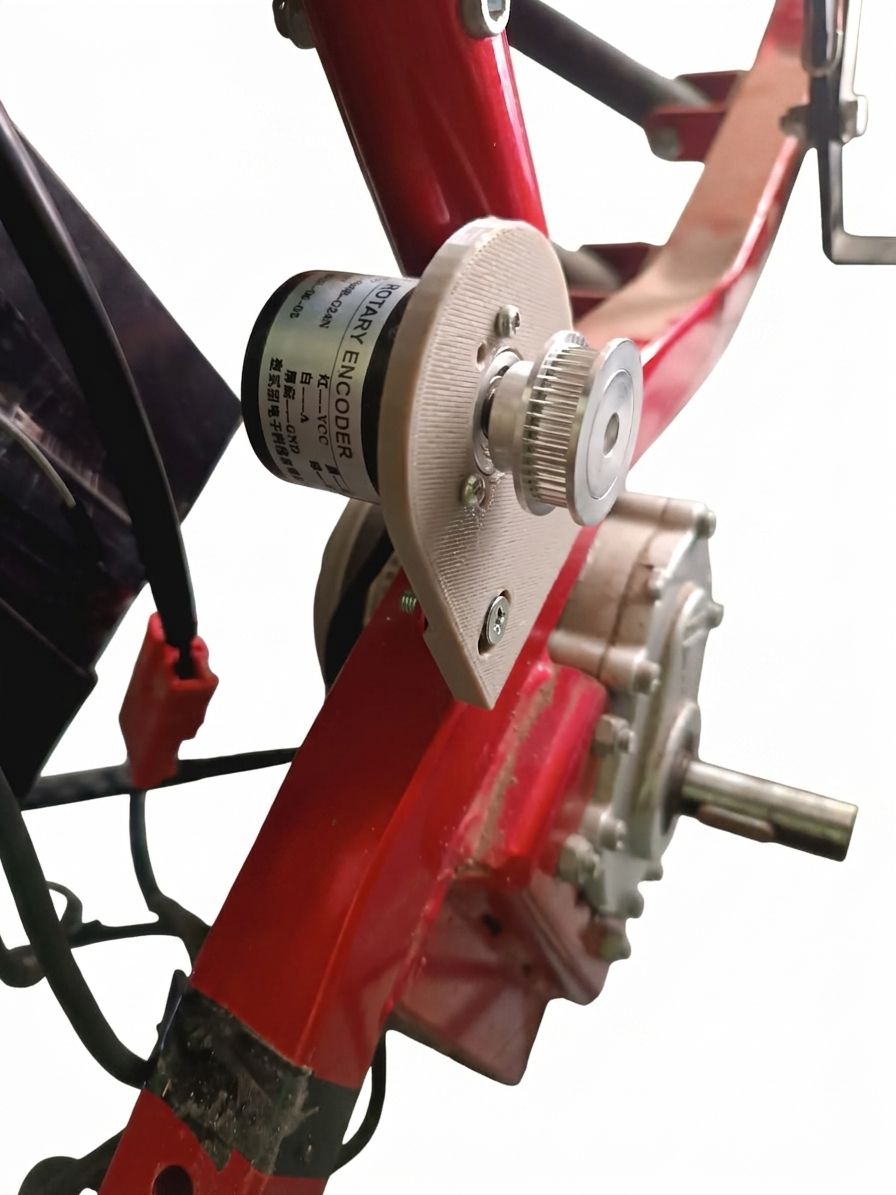
\includegraphics[height=0.22\textheight,keepaspectratio]{figures/ch10/encoder-holder-real}
        \caption{Printed part installed on the chassis.}
        \label{fig:encoder-holder-real}
    \end{subfigure}
    \caption{Encoder holder: (a) 3D CAD model, (b) printed part installed on the chassis.}
    \label{fig:encoder-holder}
\end{figure}

The bracket shown in Figure~\ref{fig:encoder-holder} holds the encoder shaft parallel to the wheel axle so the GT2 belt runs flat with no lateral misalignment.



\subsection*{GT2 Transmission}
To improve wheel speed measurement accuracy and odometry estimation, the wheel encoders were not mounted directly on the motor shafts. Instead, a mechanical transmission system based on a GT2 timing belt and two pulleys was designed to connect the motor shaft to the encoder.

The transmission system consists of:
\begin{itemize}
\item A 129-tooth GT2 pulley mounted on the wheelchair wheel shaft.
\item A 40-tooth GT2 pulley mounted on the encoder shaft.
\item A GT2 timing belt connecting both pulleys.
\end{itemize}

\begin{figure}[H]
    \centering
    \begin{subfigure}[t]{0.48\textwidth}
        \centering
        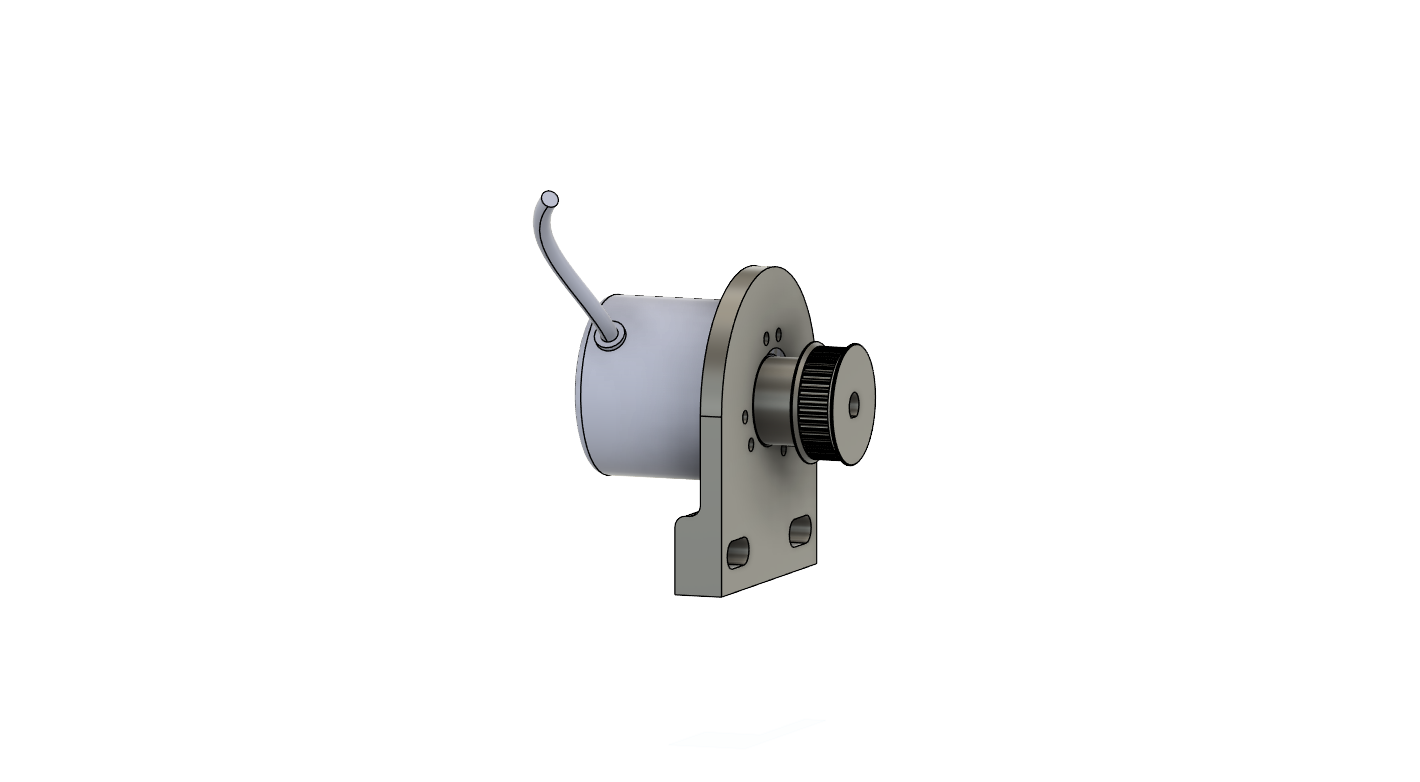
\includegraphics[height=0.20\textheight,keepaspectratio]{figures/ch10/gt2-transmission-cad-assembly}
        \caption{40-tooth GT2 pulley mounted on the encoder shaft.}
        \label{fig:gt2-transmission-cad-assembly}
    \end{subfigure}
    \hfill
    \begin{subfigure}[t]{0.48\textwidth}
        \centering
        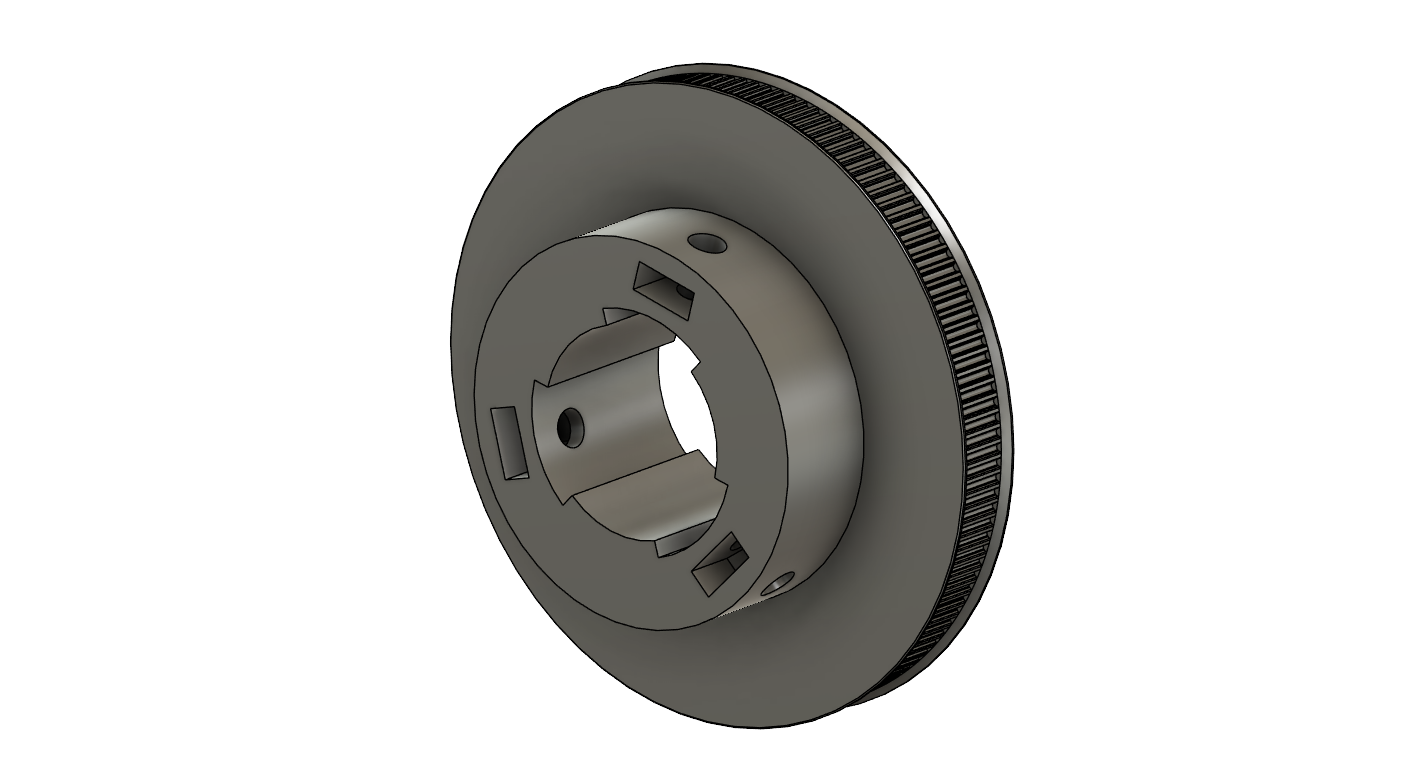
\includegraphics[height=0.20\textheight,keepaspectratio]{figures/ch10/gt2-transmission-real}
        \caption{129-tooth GT2 pulley mounted on the wheel shaft.}
        \label{fig:gt2-transmission-real}
    \end{subfigure}

    \vspace{0.6cm}

    \begin{subfigure}[t]{0.65\textwidth}
        \centering
        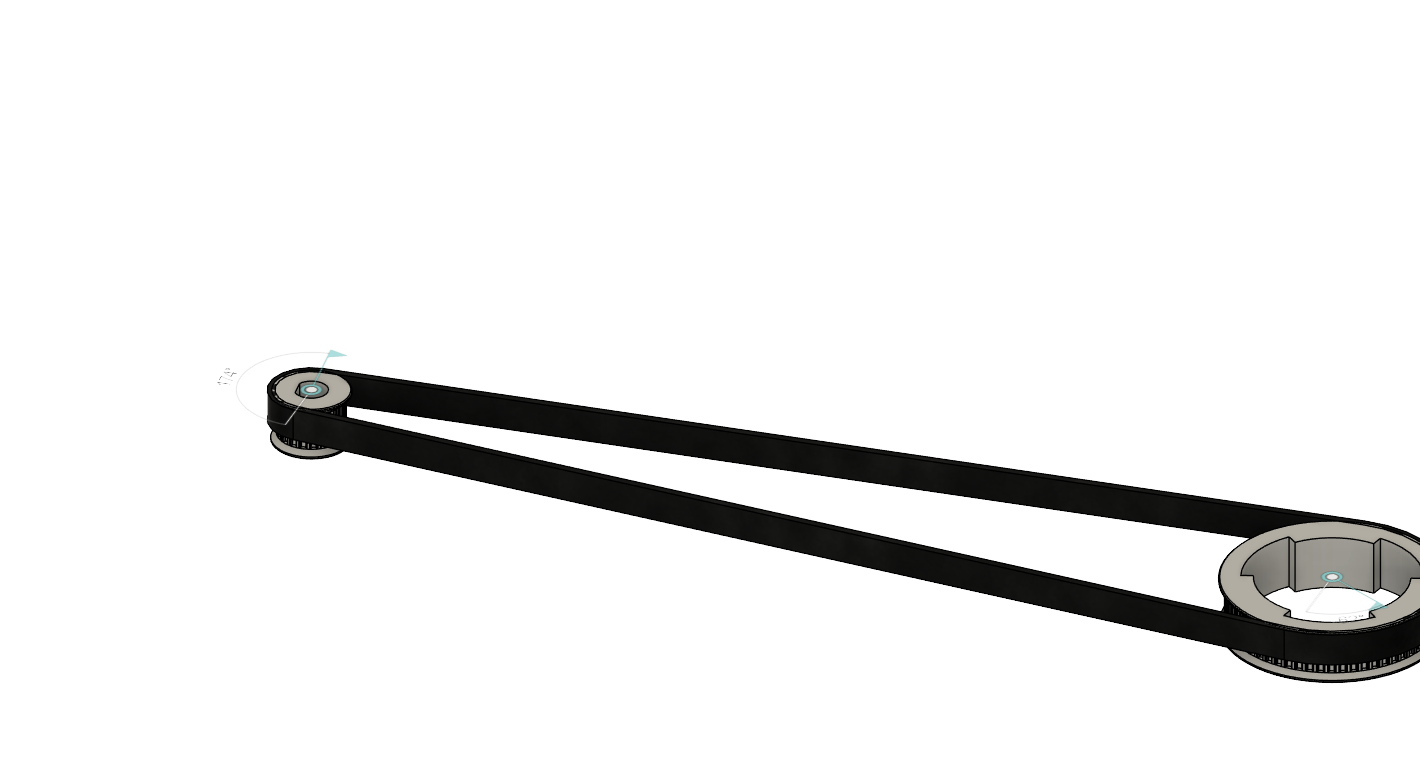
\includegraphics[height=0.20\textheight,keepaspectratio]{figures/ch10/gt2-transmission-cad-exploded}
        \caption{Assembly view showing the 129T and 40T pulleys connected by the belt.}
        \label{fig:gt2-transmission-cad-exploded}
    \end{subfigure}
    \caption{GT2 pulley--belt transmission, CAD models: (a) 40-tooth pulley on the encoder shaft, (b) 129-tooth pulley on the wheel shaft, (c) assembled transmission showing both pulleys connected by the belt.}
    \label{fig:gt2-transmission}
\end{figure}
The 3.225:1 ratio between the 129-tooth and 40-tooth pulleys shown in Figure~\ref{fig:gt2-transmission} is easier to verify visually when each pulley is inspected on its own before seeing both connected by the belt, as in the assembly view above.

The transmission ratio is calculated as:
\[
\text{Gear Ratio} = \frac{129}{40} = 3.225
\]
This means that for every complete revolution of the wheelchair wheel, the encoder rotates approximately 3.225 revolutions. Since the encoder provides 600 pulses per revolution, the effective wheel resolution becomes:
\[
\text{Effective Resolution} = 600 \times \frac{129}{40} = 1935\ \text{pulses per wheel revolution}
\]
Advantages of the GT2 belt transmission:
\begin{itemize}
\item Increases encoder measurement resolution.
\item Improves wheel velocity estimation accuracy.
\item Enhances odometry precision for SLAM and localization.
\end{itemize}
The use of a GT2 timing belt transmission allows the encoder to operate at a higher rotational
speed than the wheel, effectively multiplying the encoder resolution by a factor of 3.225. This
significantly improves the performance of the PID speed controller and the accuracy of wheel
odometry, both of which are critical for reliable autonomous navigation of the smart wheelchair.

\subsection*{Motor Driver Installation}
Two BTS7960 motor drivers were mounted beneath the wheelchair seat, close to the motors, to minimize cable length and voltage drop. Each driver independently controls one of the two 24 V, 250 W brushed DC motors, enabling differential drive and precise speed regulation of the left and right wheels. The drivers receive PWM and direction signals from the Arduino Nano, which executes the motor control algorithm and processes the encoder feedback. Figure~\ref{fig:motor-driver} shows the motor driver board installed beneath the seat.

\begin{figure}[H]
    \centering
    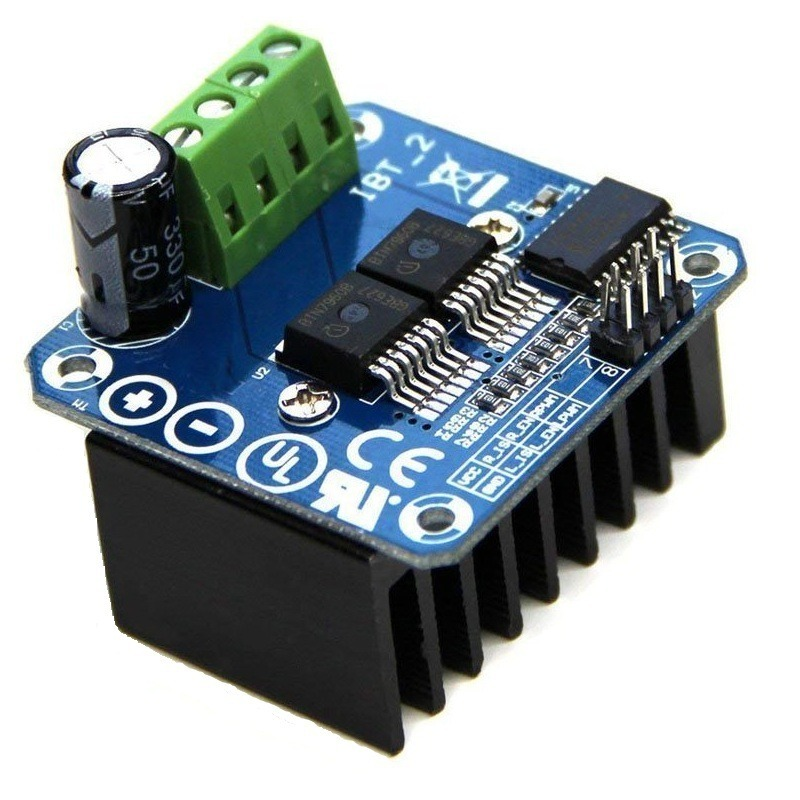
\includegraphics[height=0.18\textheight,keepaspectratio]{figures/ch10/motor-driver}
    \caption{Motor driver board installed under the wheelchair seat.}
    \label{fig:motor-driver}
\end{figure} 
\subsection{Assistive Module Integration}

In addition to the core navigation and mobility subsystems, several modular assistive devices were integrated into the Sanad smart wheelchair to enhance accessibility, usability, and healthcare support. These modules were designed using a plug-and-play architecture, allowing them to be added, removed, or upgraded independently without affecting the operation of the main wheelchair system.

The modular approach provides flexibility to adapt the wheelchair to the specific needs of different users. Depending on the user's physical condition and requirements, assistive modules such as head-motion control, touchscreen interaction, and biometric health monitoring can be enabled or disabled as needed.

\subsection*{Head-Motion Control Unit}
A wearable IMU module was mounted on a head strap, allowing users with limited hand mobility to control the wheelchair through head movements. The sensor continuously measures the orientation and angular motion of the user's head and converts these measurements into navigation commands such as forward motion, turning left, turning right, and stopping. This hands-free control approach provides an alternative interaction method for users who may be unable to operate conventional joysticks or touch interfaces due to physical impairments. The head-mounted configuration ensures stable sensor positioning relative to the user's head, improving measurement accuracy and reducing motion artifacts caused by body movements. Figure~\ref{fig:head-control-unit} shows the wearable IMU head control module.

% TODO (pending clarification): another possible candidate for the "space below /
% merge the a-b figure into it" request. Not applied yet.
\begin{figure}[H]
    \centering
    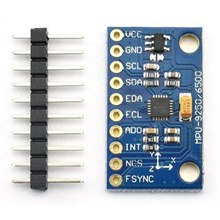
\includegraphics[height=0.18\textheight,keepaspectratio]{figures/ch10/head-control-unit}
    \caption{Wearable IMU head control module.}
    \label{fig:head-control-unit}
\end{figure}

\begin{figure}[H]
    \centering
    \begin{subfigure}[t]{0.48\textwidth}
        \centering
        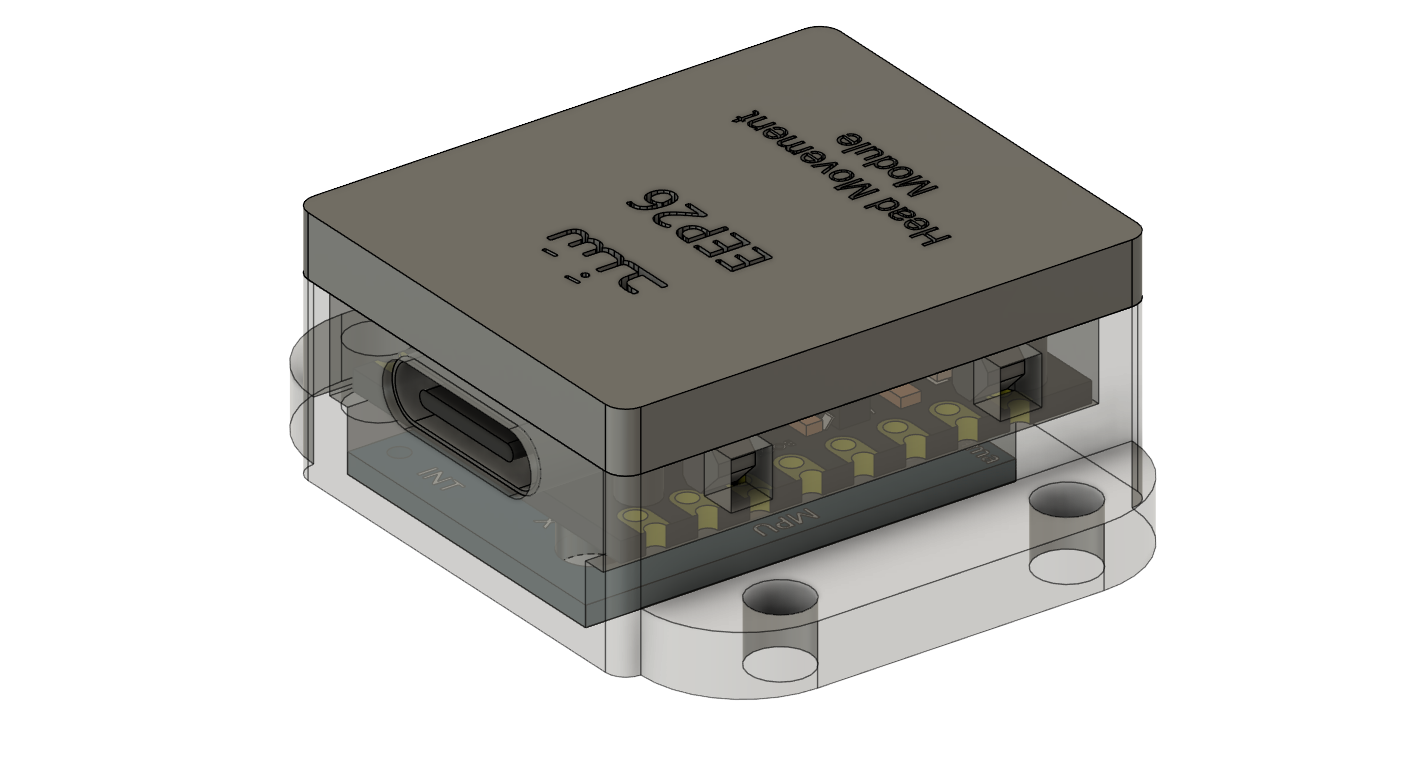
\includegraphics[height=0.20\textheight,keepaspectratio]{figures/ch10/head-unit-cad-front}
        \caption{CAD front view of the shell.}
        \label{fig:head-unit-cad-front}
    \end{subfigure}\hfill
    \begin{subfigure}[t]{0.48\textwidth}
        \centering
        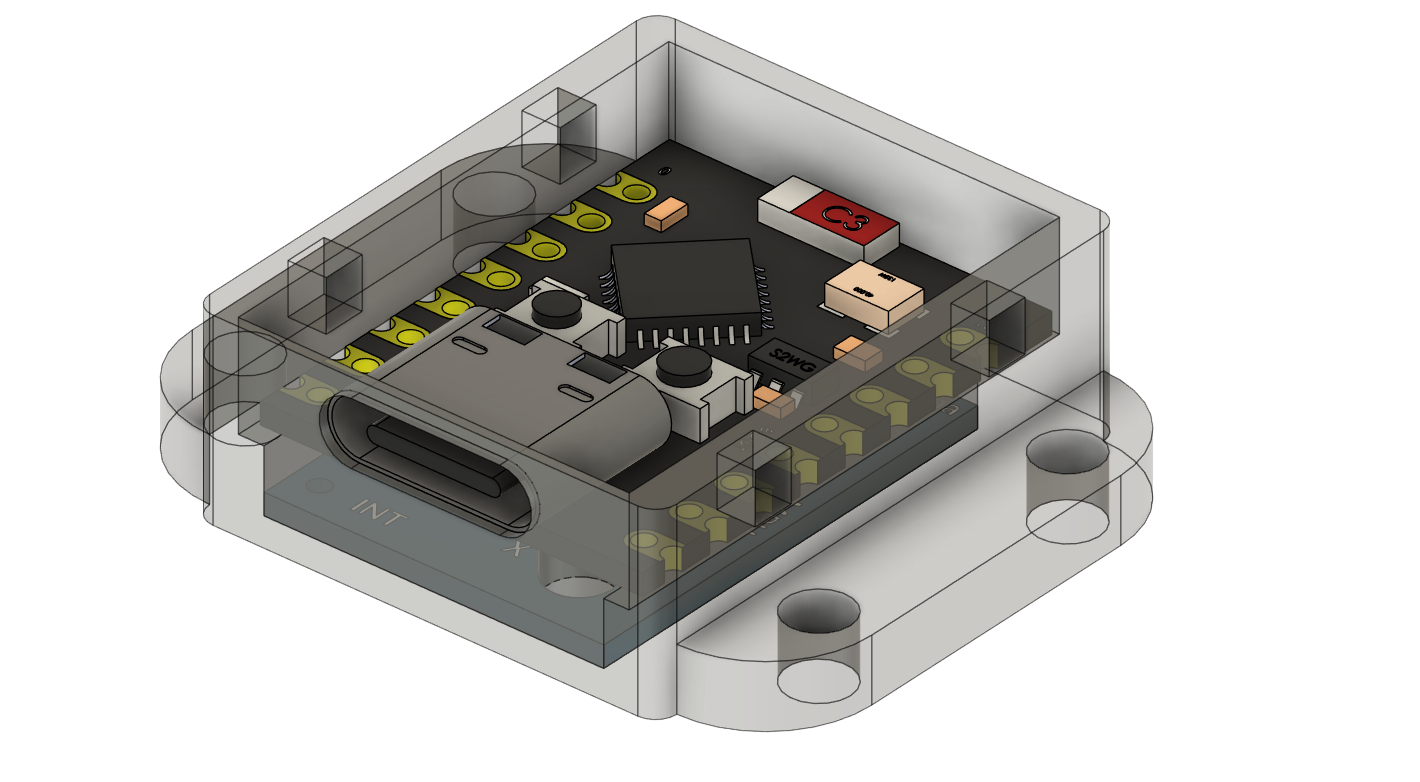
\includegraphics[height=0.20\textheight,keepaspectratio]{figures/ch10/head-unit-cad-internal}
        \caption{CAD exploded view showing IMU seating.}
        \label{fig:head-unit-cad-internal}
    \end{subfigure}

    \vspace{0.6cm}


    \caption{Wearable head-motion control unit: (a) CAD front view of the shell, (b) CAD exploded view showing IMU seating}
    \label{fig:head-unit}
\end{figure}

The wearable head-motion control unit shown in Figure~\ref{fig:head-unit} houses the IMU board, wiring, and strap clip inside a single shell; the exploded view is included because that internal arrangement is not visible from the exterior alone.

\subsection*{Touchscreen Mount}
A 10-inch touchscreen was mounted on the right armrest using a foldable 3D-printed support structure.
\begin{itemize}
\item Goal selection.
\item Navigation interface.
\item Settings configuration.
\item Eye tracking interface.
\end{itemize}
% TODO (pending clarification): another possible candidate for the "space below /
% merge the a-b figure into it" request. Not applied yet.
Figure~\ref{fig:touchscreen-mount} shows the touchscreen mounted on the wheelchair armrest.
\begin{figure}[tbp]
    \centering
    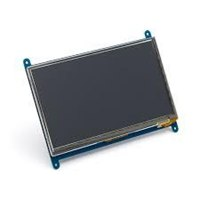
\includegraphics[width=\linewidth,height=0.18\textheight,keepaspectratio]{figures/ch10/touchscreen-mount}
    \caption{Touchscreen mounted on the wheelchair armrest.}
    \label{fig:touchscreen-mount}
\end{figure}
\begin{figure}[tbp]
    \centering
    \begin{subfigure}[t]{0.48\textwidth}
        \centering
        
\includegraphics[width=\linewidth,height=0.20\textheight,keepaspectratio]{figures/ch10/touchscreen-holder-cad-folded}
        \caption{CAD, folded position.}
        \label{fig:touchscreen-holder-cad-folded}
    \end{subfigure}
    \hfill
    \begin{subfigure}[t]{0.48\textwidth}
        \centering
        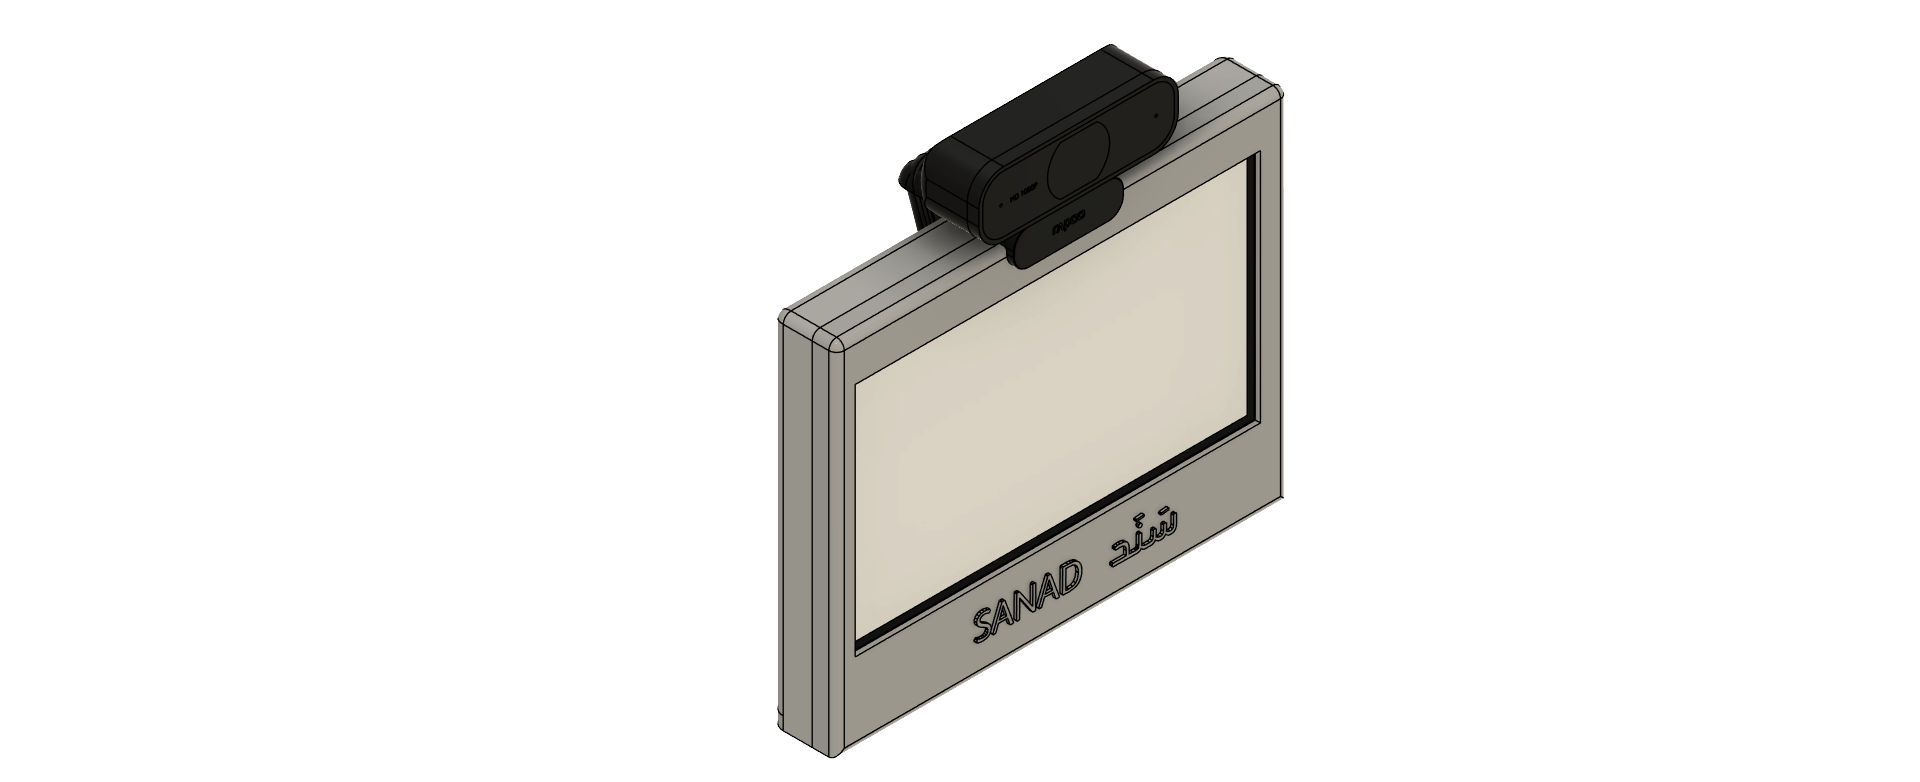
\includegraphics[width=\linewidth,height=0.20\textheight,keepaspectratio]{figures/ch10/touchscreen-holder-cad-unfolded}
        \caption{CAD, unfolded/deployed position.}
        \label{fig:touchscreen-holder-cad-unfolded}
    \end{subfigure}
    \medskip
    \begin{subfigure}[t]{0.48\textwidth}
        \centering
        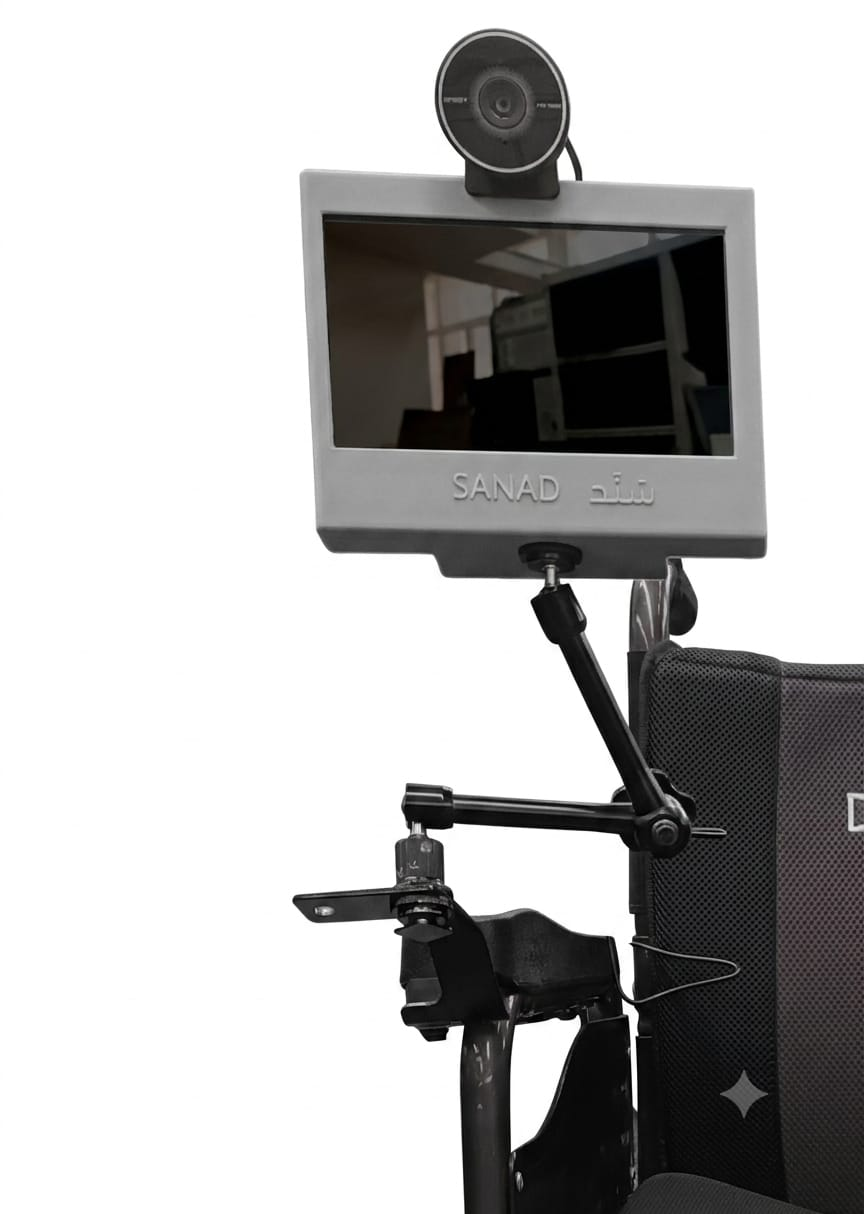
\includegraphics[width=\linewidth,height=0.20\textheight,keepaspectratio]{figures/ch10/:touchscreen-holder-real}
        \caption{Printed part on the armrest.}
        \label{fig:touchscreen-holder-real}
    \end{subfigure}
    \caption{Touchscreen holder: (a) CAD, folded position, (b) CAD, unfolded/deployed position, (c) printed part installed on the armrest.}
    \label{fig:touchscreen-holder}
\end{figure}
The hinge mechanism shown in Figures~\ref{fig:touchscreen-holder-cad-folded} and~\ref{fig:touchscreen-holder-cad-unfolded} lets the screen fold flat against the armrest for storage and swing up into its deployed position for use. Figure~\ref{fig:touchscreen-holder-real} shows the printed bracket installed and holding the screen in place.
\FloatBarrier

\subsection{Complete System Integration}

The complete integrated design was modeled in Autodesk Fusion before fabrication, allowing every sensor mount and cable route to be checked for interference prior to printing.

\begin{figure}[H]
    \centering
    \begin{subfigure}[t]{0.48\textwidth}
        \centering
        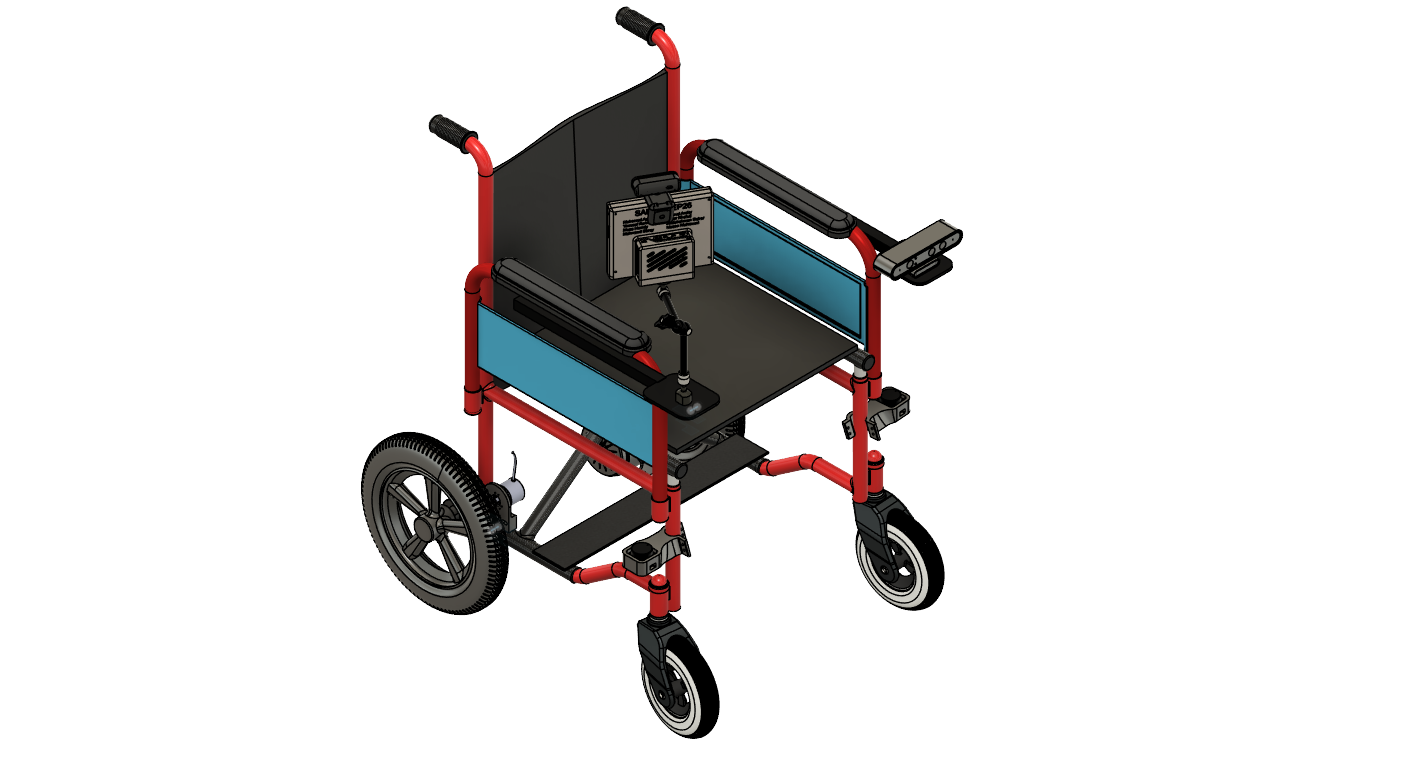
\includegraphics[height=0.28\textheight,keepaspectratio]{figures/ch10/full-wheelchair-cad-front}
        \caption{Front/isometric view.}
        \label{fig:full-wheelchair-cad-front}
    \end{subfigure}\hfill
    \begin{subfigure}[t]{0.48\textwidth}
        \centering
        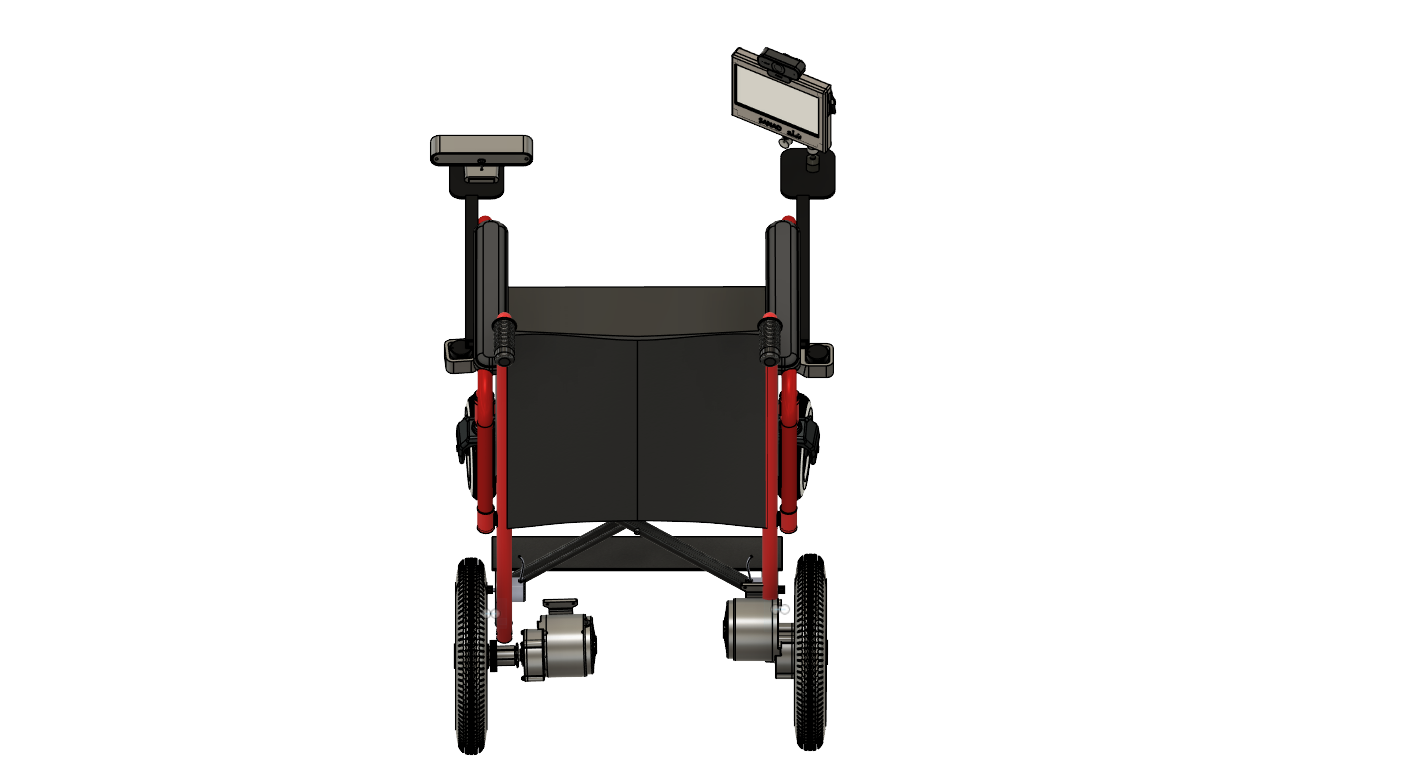
\includegraphics[height=0.28\textheight,keepaspectratio]{figures/ch10/full-wheelchair-cad-rear}
        \caption{Rear view.}
        \label{fig:full-wheelchair-cad-rear}
    \end{subfigure}
    \caption{Complete Sanad wheelchair -- CAD assembly: (a) front/isometric view, (b) rear view.}
    \label{fig:full-wheelchair-cad}
\end{figure}

Figure~\ref{fig:full-wheelchair-cad} shows the full CAD assembly with the dual LiDAR bar, depth camera, IMU, touchscreen, motor drivers, and rear-mounted encoders in their final relative positions.

\begin{figure}[H]
    \centering
    \begin{subfigure}[t]{0.48\textwidth}
        \centering
        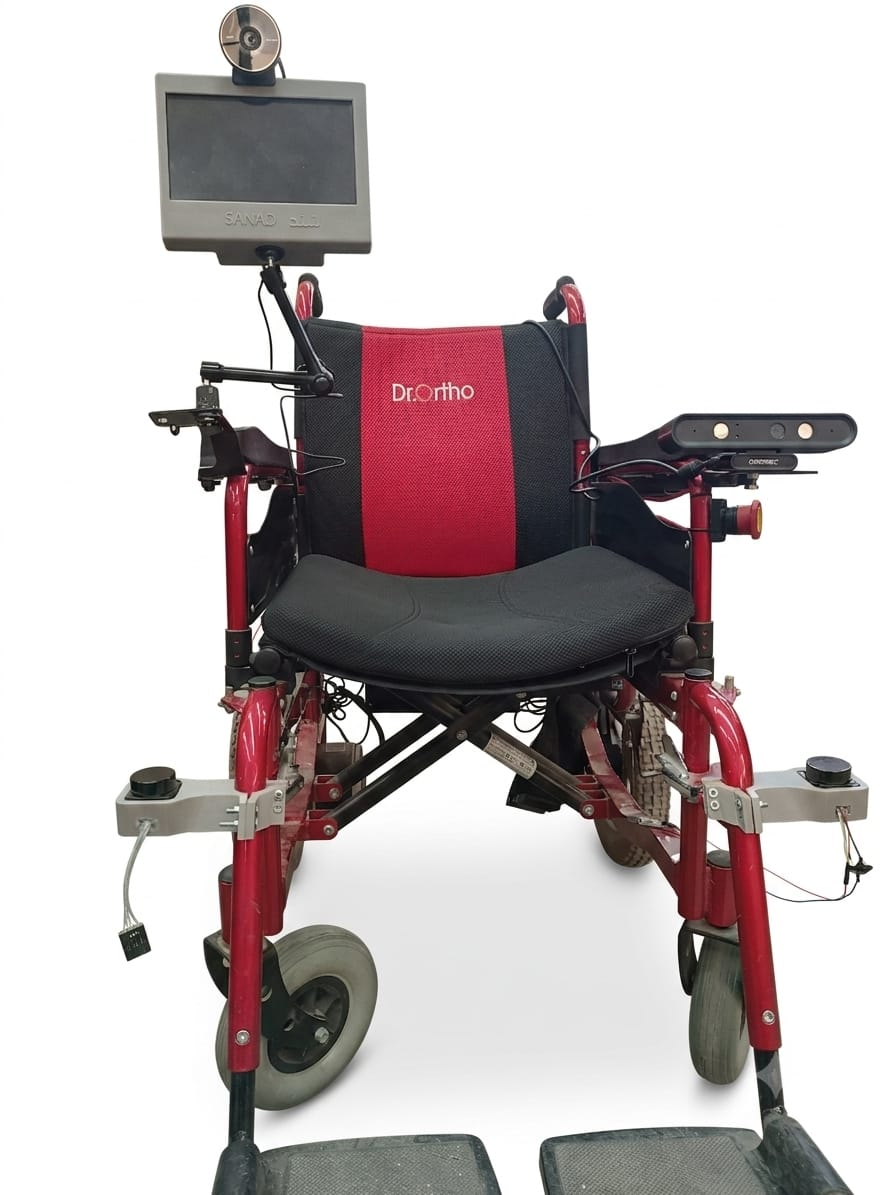
\includegraphics[height=0.28\textheight,keepaspectratio]{figures/ch10/full-wheelchair-real-front}
        \caption{Front view.}
        \label{fig:full-wheelchair-real-front}
    \end{subfigure}\hfill
    
    
    \label{fig:full-wheelchair-real}
\end{figure}

Figure~\ref{fig:full-wheelchair-real} shows the fully assembled wheelchair after all modules were installed, matching the CAD design shown above.

\section{Drivetrain Design Calculations}
This section presents the mechanical calculations used to verify that the drivetrain can safely carry the intended passenger load under normal operating conditions. The analysis is based on the rated motor power, wheel geometry, and rolling resistance, and is used to define a safe maximum payload for the wheelchair.

\subsection*{Design Data}

Table~\ref{tab:design-data} lists the key design parameters used in the calculations that follow.

\begin{table}[H]
\centering
\caption{The key design parameters used in the calculations are}
\label{tab:design-data}
\begin{tabular}{l c c c}
\hline
Parameter& Value  \\
\hline
Rated Power & 250W  \\
Maximum Speed & 8 km/h (2.22 m/s)\\
Wheel Radius &127 mm \\
Wheelchair Mass& 46 kg  \\
Rolling Resistance Coefficient & 0.06 \\
Factor of Safety & 1.2 \\
\hline
\end{tabular}
\end{table}


\subsection*{Assumptions}
The following simplifying assumptions were adopted to keep the analysis tractable while remaining representative of typical indoor operating conditions:
\begin{itemize}
\item Level ground.
\item Constant speed.
\item Rolling resistance only (aerodynamic drag and grade resistance neglected).
\item Rated power available at the wheels.
\end{itemize}

\subsection*{Calculations}
Using the design data in Table~\ref{tab:design-data} and the assumptions above, the wheel torque, tractive force, and maximum safe payload were calculated as follows.
\[
\omega = \frac{v}{r} = \frac{2.22}{0.127} = 17.5\ \mathrm{rad/s}
\]
\[
T = \frac{P}{\omega} = \frac{250}{17.5} = 14.3\ \mathrm{N\,m}
\]
\[
F = \frac{T}{r} = 112.6\ \mathrm{N}
\]
Rolling resistance force:
\[
F_{rr} = \mu (46 + m_{\text{load}}) g
\]
Setting the tractive force equal to the rolling resistance force and solving for the load mass gives a theoretical maximum passenger load of approximately 145.3\,kg. Applying the factor of safety of 1.2 gives the recommended design passenger load of approximately 121.1\,kg.

A factor of safety of 1.2 was selected because the wheelchair is intended for indoor operation on smooth, level floors under controlled loading conditions. This safety margin accounts for minor variations in rolling resistance, drivetrain efficiency, battery performance, and manufacturing tolerances while avoiding excessive oversizing.
\subsection*{Conclusion}
Based on the assumed operating conditions, the theoretical maximum passenger load is
approximately 145.3 kg. Applying a factor of safety of 1.2 gives a recommended design
passenger load of approximately 121 kg, which is consistent with the manufacturer's rated
capacity of 120 kg for the base wheelchair platform.

\subsection*{Motor Calculations}

The rated current of one DC motor is calculated from the rated power and supply voltage as

\[
I_{\text{rated}}=\frac{P}{V}
=\frac{250}{24}
=10.4~\mathrm{A}
\]

In practice, during normal indoor driving at moderate speeds, DC wheelchair motors typically draw only 20--50\% of their rated current. Therefore, the expected operating current of one motor is

\[
I_{\text{motor (normal)}} \approx 4\text{--}6~\mathrm{A}
\]

For two motors, the total operating current becomes

\[
I_{\text{total (normal)}} \approx 8\text{--}12~\mathrm{A}
\]

At startup, DC brushed motors typically draw approximately three times their rated current. Assuming a startup factor of 3,

\[
I_{\text{start}}
=3\times10.4
=31.2~\mathrm{A}
\]

The wheelchair uses two BTS7960 motor drivers, each capable of handling approximately \(43~\mathrm{A}\) peak current. Therefore,

\[
31.2~\mathrm{A}<43~\mathrm{A}
\]

which satisfies the current handling capability of the motor driver.    
\section{Motor Control \& PID Tuning}
The wheelchair utilizes two BTS7960 high-current motor drivers controlled by an Arduino Nano microcontroller to regulate the speed and direction of the two drive motors. Wheel velocity feedback is obtained from the wheel encoders, enabling the implementation of a closed-loop speed control system based on a PID controller.
\subsection*{Control Loop}
Figure~\ref{fig:control-loop} illustrates the complete end-to-end motor control loop, starting from the \texttt{cmd\_vel} velocity command generated by the navigation stack, through the PID controller and motor driver, to the DC motor. Encoder feedback is continuously returned to the controller, forming a closed-loop control system that ensures accurate speed regulation and reliable motor performance.

\begin{figure}[H]
\centering
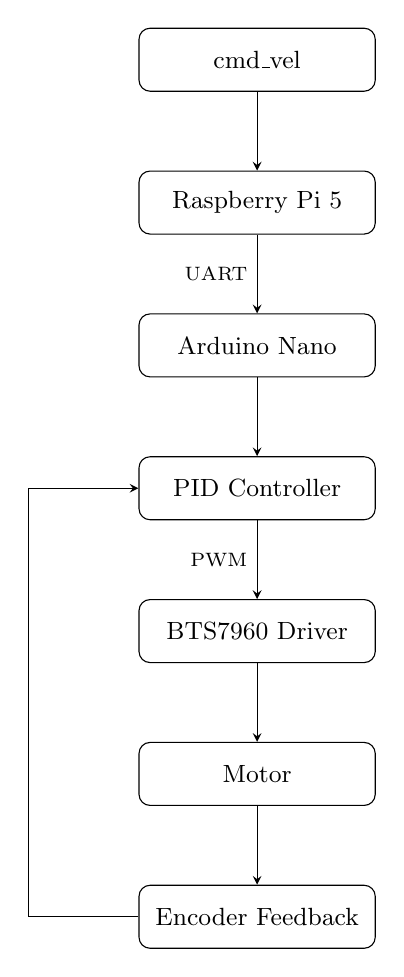
\begin{tikzpicture}[>=stealth, node distance=10mm, every node/.style={font=\small}]
\tikzstyle{block}=[draw, rounded corners, minimum width=3cm, minimum height=8mm, align=center]
\node[block] (cmdvel) {cmd\_vel};
\node[block, below=of cmdvel] (rpi) {Raspberry Pi 5};
\node[block, below=of rpi] (nano) {Arduino Nano};
\node[block, below=of nano] (pid) {PID Controller};
\node[block, below=of pid] (driver) {BTS7960 Driver};
\node[block, below=of driver] (motor) {Motor};
\node[block, below=of motor] (encoder) {Encoder Feedback};

\draw[->] (cmdvel) -- (rpi);
\draw[->] (rpi) -- node[left, font=\scriptsize]{UART} (nano);
\draw[->] (nano) -- (pid);
\draw[->] (pid) -- node[left, font=\scriptsize]{PWM} (driver);
\draw[->] (driver) -- (motor);
\draw[->] (motor) -- (encoder);
\draw[->] (encoder.west) -| ++(-1.4,0) |- (pid.west);
\end{tikzpicture}
\caption{End-to-end motor control loop from cmd\_vel to encoder feedback.}
\label{fig:control-loop}
\end{figure}
The Raspberry Pi 5 generates the desired wheel velocities through the \texttt{cmd\_vel} command and transmits them to the Arduino Nano via serial (UART) communication. The Arduino compares the desired velocity with the actual wheel speed measured by the encoders and computes the control signal using the PID algorithm. The resulting PWM signal is then sent to the BTS7960 motor driver to regulate the motor speed.


\subsection*{PID Structure}
The Arduino Nano implements a discrete PID controller for each wheel that converts the velocity error into a PWM duty-cycle command. Figure~\ref{fig:pid-structure} shows the general structure of this control loop. The PID controller output is:
\[
u(t) = K_p e(t) + K_i \int e(t)\,dt + K_d \frac{d e(t)}{dt}
\]
where
\[
e(t) = \text{setpoint} - \text{measured value}.
\]

Proportional control reacts to the current error. Increasing $K_p$ generally produces a faster response and smaller error, while too large a value can cause oscillation. Integral control accumulates past errors, removing steady-state error and helping the motor reach the target RPM; however, too much integral gain can lead to overshoot and oscillation. Derivative control predicts future behavior based on the error rate of change, reducing overshoot and improving stability.

\begin{figure}[H]
\centering
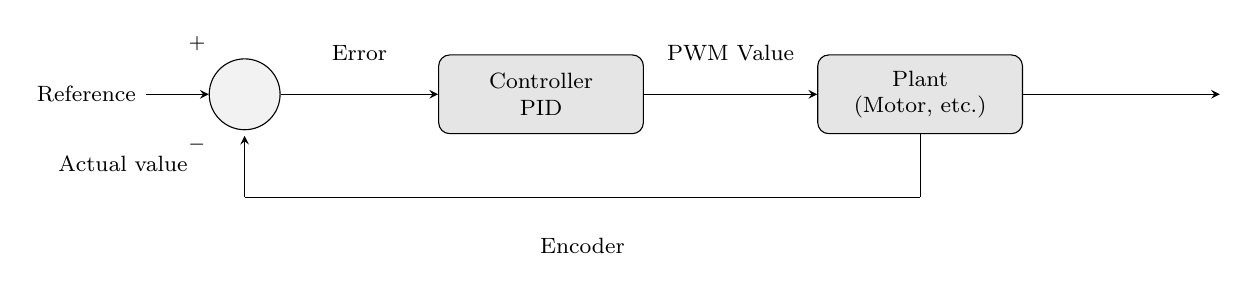
\begin{tikzpicture}[>=stealth,node distance=20mm,every node/.style={font=\footnotesize}]
\tikzstyle{block}=[draw,fill=gray!20,rounded corners,minimum width=2.6cm,minimum height=1cm,align=center]
\tikzstyle{sum}=[draw,circle,fill=gray!10,minimum size=9mm,inner sep=0pt]

\node[sum] (sum) {};
\node[left=8mm of sum] (ref) {Reference};
\node[above left=1mm and .5mm of sum,font=\scriptsize] {$+$};
\node[below left=1mm and .5mm of sum,font=\scriptsize] {$-$};

\node[block,right=20mm of sum] (pid) {Controller\\PID};
\node[block,right=22mm of pid] (plant) {Plant\\(Motor, etc.)};

\draw[->] (ref) -- (sum);
\draw[->] (sum) -- node[midway,above=3mm]{Error} (pid);
\draw[->] (pid) -- node[midway,above=3mm]{PWM Value} (plant);
\draw[->] (plant.east) -- ++(25mm,0);

\coordinate (corner) at ($(plant.south)+(0,-8mm)$);
\coordinate (fb) at ($(sum.south |- corner)$);

\draw (plant.south) -- (corner);
\draw (corner) -- node[midway,below=4mm]{Encoder} (fb);
\draw[->,shorten >=2pt] (fb) -- node[midway,left=6mm]{Actual value} (sum.south);

\end{tikzpicture}
\caption{General PID control loop structure used for wheel speed control.}
\label{fig:pid-structure}
\end{figure}
\subsection*{The PID controller output is:}
\[
u(t)=K_p\,e(t)+K_i\int_{0}^{t}e(\tau)\,d\tau+K_d\frac{de(t)}{dt}
\]
\subsection*{Where:}
\begin{itemize}
    \item P = Proportional term
    \item I = Integral term
    \item  D = Derivative term
    \item  e(t): Control error, defined as:
     e(t) = setpoint − measured value
\end{itemize}

\begin{enumerate}
    \item \textbf{Proportional Control (P)} \\
   \\ The proportional term reacts to the current error.\\
   \textbf{Effect of increasing Kp:} 
   \begin{itemize}
       \item Faster response.
       \item Smaller steady-state error.
       \item Too large → oscillation
   \end{itemize}

Figure~\ref{fig:kp-effect} illustrates the effect of increasing $K_p$ on the speed response.

\begin{figure}[H]
\centering
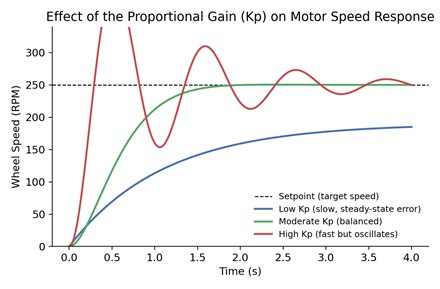
\includegraphics[width=0.5\linewidth,keepaspectratio]{figures/ch10/kp-effect}
\caption{Illustrative effect of increasing proportional gain on the speed response.}
\label{fig:kp-effect}
\end{figure}

\item \textbf{Integral Control (I)} \\
    \\The integral term accumulates and remembers past errors.
    \\  \textbf{Effect of increasing KI:} 
     \begin{itemize}
       \item Removes steady-state error.
       \item Helps the motor reach exactly the target RPM.
       \item Too high → overshoot and oscillation.
   \end{itemize}

Figure~\ref{fig:ki-effect} illustrates the effect of increasing $K_i$ on the steady-state error.

\begin{figure}[H]
\centering
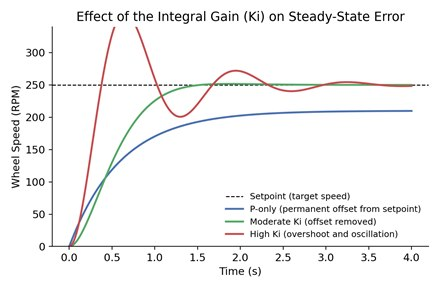
\includegraphics[width=0.5\linewidth,keepaspectratio]{figures/ch10/ki-effect}
\caption{Illustrative effect of integral gain on steady-state error.}
\label{fig:ki-effect}
\end{figure}
 \item \textbf{Derivative Control (D)} \\
    \\The derivative term predicts future behavior by looking at how fast the error changes.
    \\  \textbf{Effect of increasing Kd:} 
     \begin{itemize}
       \item Reduces overshoot.
       \item Improves stability.
   \end{itemize}
     \end{enumerate}

Figure~\ref{fig:kd-effect} illustrates the effect of increasing $K_d$ on overshoot and stability.

\begin{figure}[H]
\centering
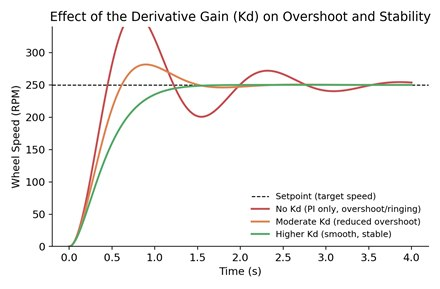
\includegraphics[width=0.5\linewidth,keepaspectratio]{figures/ch10/kd-effect}
\caption{Illustrative effect of derivative gain on overshoot and stability.}
\label{fig:kd-effect}
\end{figure}

% ============================================================
% EDIT: The Ziegler--Nichols tuning subsection below has been commented out
% and replaced with a trial-and-error tuning subsection, per user request.
% ============================================================
% \subsection*{PID Tuning Using the Ziegler--Nichols Method}
% The PID controller parameters were initially tuned using the Ziegler--Nichols closed-loop tuning method, which provides a systematic approach for estimating controller gains.
%
% The tuning procedure consists of the following steps:
% \begin{enumerate}
% \item Set the integral and derivative gains to zero: $K_i = 0$, $K_d = 0$.
% \item Gradually increase the proportional gain $K_p$ until the motor output exhibits continuous and stable oscillations.
% \item Record the proportional gain at which sustained oscillation occurs. This value is known as the Ultimate Gain ($K_u$).
% \item Measure the oscillation period, known as the Ultimate Period ($P_u$).
% \item Compute the PID parameters using the Ziegler--Nichols tuning rules:
% \end{enumerate}
% \begin{itemize}
%     \item $K_p = 0.6 K_u$, 
%     \item $K_i = 2 K_p / P_u$,
%     \item $K_d = K_p P_u / 8$.
%
% \end{itemize}
%
% \subsection*{Advantages of using Ziegler–Nichols tuning}
% \begin{itemize}
%     \item Provides a systematic and repeatable tuning procedure.
%     \item Produces reasonable initial gain values without requiring an accurate mathematical
% model
%     \item Reduces manual trial-and-error tuning efforts.
%     \item Enables rapid deployment of the motor control system.
%     \item Serves as an effective starting point for further experimental optimization.
% \end{itemize}

\subsection*{PID Tuning Using a Trial-and-Error Method}
The PID controller parameters were tuned experimentally using a manual trial-and-error approach.

The tuning procedure consists of the following steps:
\begin{enumerate}
\item Start with only the proportional gain enabled ($K_i = 0$, $K_d = 0$) and gradually increase $K_p$ while observing the wheel speed response, until a reasonable trade-off is reached between fast response and acceptable oscillation.
\item Introduce a small integral gain $K_i$ and increase it gradually to eliminate steady-state error, so the motor reliably reaches the target RPM.
\item Add a small derivative gain $K_d$ and increase it gradually to damp any remaining oscillation and improve overall stability.
\item Repeat the above steps under different payload conditions to confirm the selected gains remain acceptable across the expected range of user weights.
\end{enumerate}

\subsection*{Advantages of the trial-and-error tuning approach}
\begin{itemize}
    \item Does not require an accurate mathematical model of the motor--wheelchair system.
    \item Allows the gains to be adjusted directly based on the observed real-world response, including nonlinearities that an analytical model would not capture.
    \item Simple to apply with basic test equipment and no specialized instrumentation.
    \item Well suited to iterative refinement of the gains across different payloads and operating conditions.
\end{itemize}





\section{Hardware Circuit \& Power System}
This section describes the electrical implementation of the wheelchair, covering both the custom motor-control interface circuit and the overall power distribution architecture. Together, these subsystems ensure that every sensor, actuator, and compute module receives clean, adequately rated power while keeping wiring between the Arduino Nano, the motor drivers, and the encoders as short and reliable as possible.

\subsection{Motor Control \& Encoder Interface Board}

A custom interface board was developed around the Arduino Nano to simplify the electrical connections between the microcontroller, the two BTS7960 motor drivers, and the dual quadrature wheel encoders. Instead of wiring each module individually, the board integrates all signal and power connections into a compact PCB with clearly labeled connectors.

The interface board includes a dedicated terminal Block power input, separate connectors for the left and right motor drivers, and dedicated headers for both wheel encoders. This arrangement minimizes wiring complexity, improves assembly reliability, simplifies maintenance, and reduces the likelihood of connection errors. The compact design also allows the complete motor control electronics to be mounted beneath the wheelchair seat alongside the motor drivers.

% TODO (pending clarification): user asked to enlarge subfigure (b) of "figure 10.99"
% so it is readable. The most likely candidate in this chapter is the electrical
% schematic below (subfigure (b) of the PCB figure), since schematics tend to have
% small text/labels, but this has NOT been resized yet -- waiting to confirm which
% figure was meant before changing its size.
Figure~\ref{fig:PCB} presents the custom interface board. The PCB layout is shown in Figure~\ref{fig:PCB}(a), while the corresponding electrical schematic is shown in Figure~\ref{fig:PCB}(b).

\begin{figure}[H]
\centering

\begin{figure}[H]
\centering
\begin{subfigure}[t]{0.55\textwidth}
    \centering
    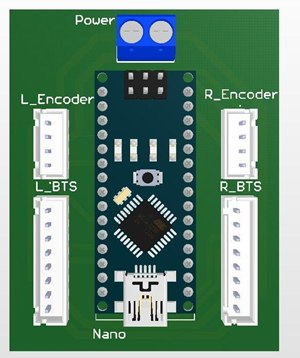
\includegraphics[width=0.8\linewidth]{figures/ch10/PCB}
    \caption{Custom PCB layout.}
\end{subfigure}

\vspace{0.3cm}

\begin{subfigure}[t]{0.9\textwidth}
    \centering
    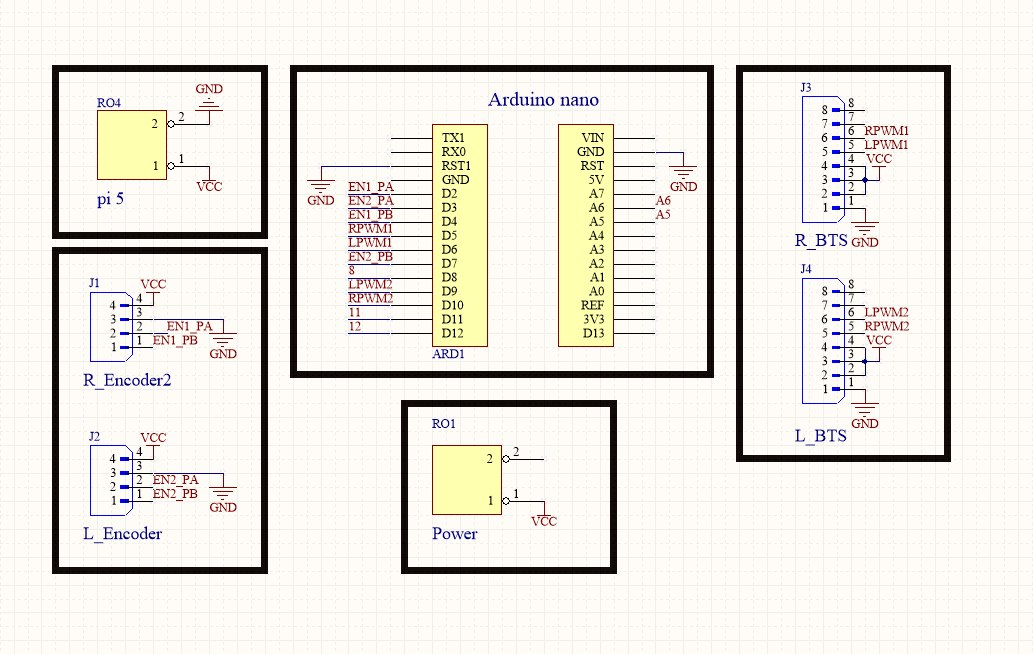
\includegraphics[width=0.85\linewidth]{figures/ch10/PCB_Schematic}
    \caption{Electrical schematic of the interface board.}
\end{subfigure}

\caption{Arduino Nano motor control and encoder interface board: (a) custom PCB layout and (b) electrical schematic.}
\label{fig:PCB}
\end{figure}
  
  \caption{Arduino Nano motor control and encoder interface board: (a) custom PCB layout and (b) electrical schematic.}
  \label{fig:PCB}
\end{figure}
\caption{Arduino Nano motor control and encoder interface board: (a) custom PCB layout and (b) electrical schematic.}
\label{fig:PCB}
\end{figure}
\subsection{Power Distribution Architecture}
Electrical power for the compute and sensing subsystems is supplied by a dedicated 12V,
23.45Ah lithium-ion battery, separate from the wheelchair's original 24V drive battery. A voltage
sensor continuously monitors this battery for health and charge-state monitoring. An inline fuse
is placed immediately after the battery's positive terminal, ahead of the branch to the voltage
sensor and the two buck converters, to protect the battery, wiring, and downstream electronics
against short-circuit and overcurrent conditions. Two buck
converters step the 12V supply down to a regulated 5V rail: a 7A converter dedicated to the
Raspberry Pi 5 main compute unit, and a 12A converter that supplies all remaining peripherals.
The 12A rail is distributed through internal USB connections to the dual LiDAR units, the depth
camera, and the Arduino Nano, through external USB connections to the head-mounted IMU, the
IR module, the hand biometric sensor, and the microphone, and through dedicated USB femaleterminals to the secondary Raspberry Pi 4 (which drives the touchscreen and eye-tracking
interface), the 7-inch screen, and the speaker output. Figure~\ref{fig:power-distribution} illustrates the complete power
distribution tree, including the protective fuse placed between the battery and the downstream loads.

\begin{figure}[H]
\centering
\resizebox{\textwidth}{!}{%
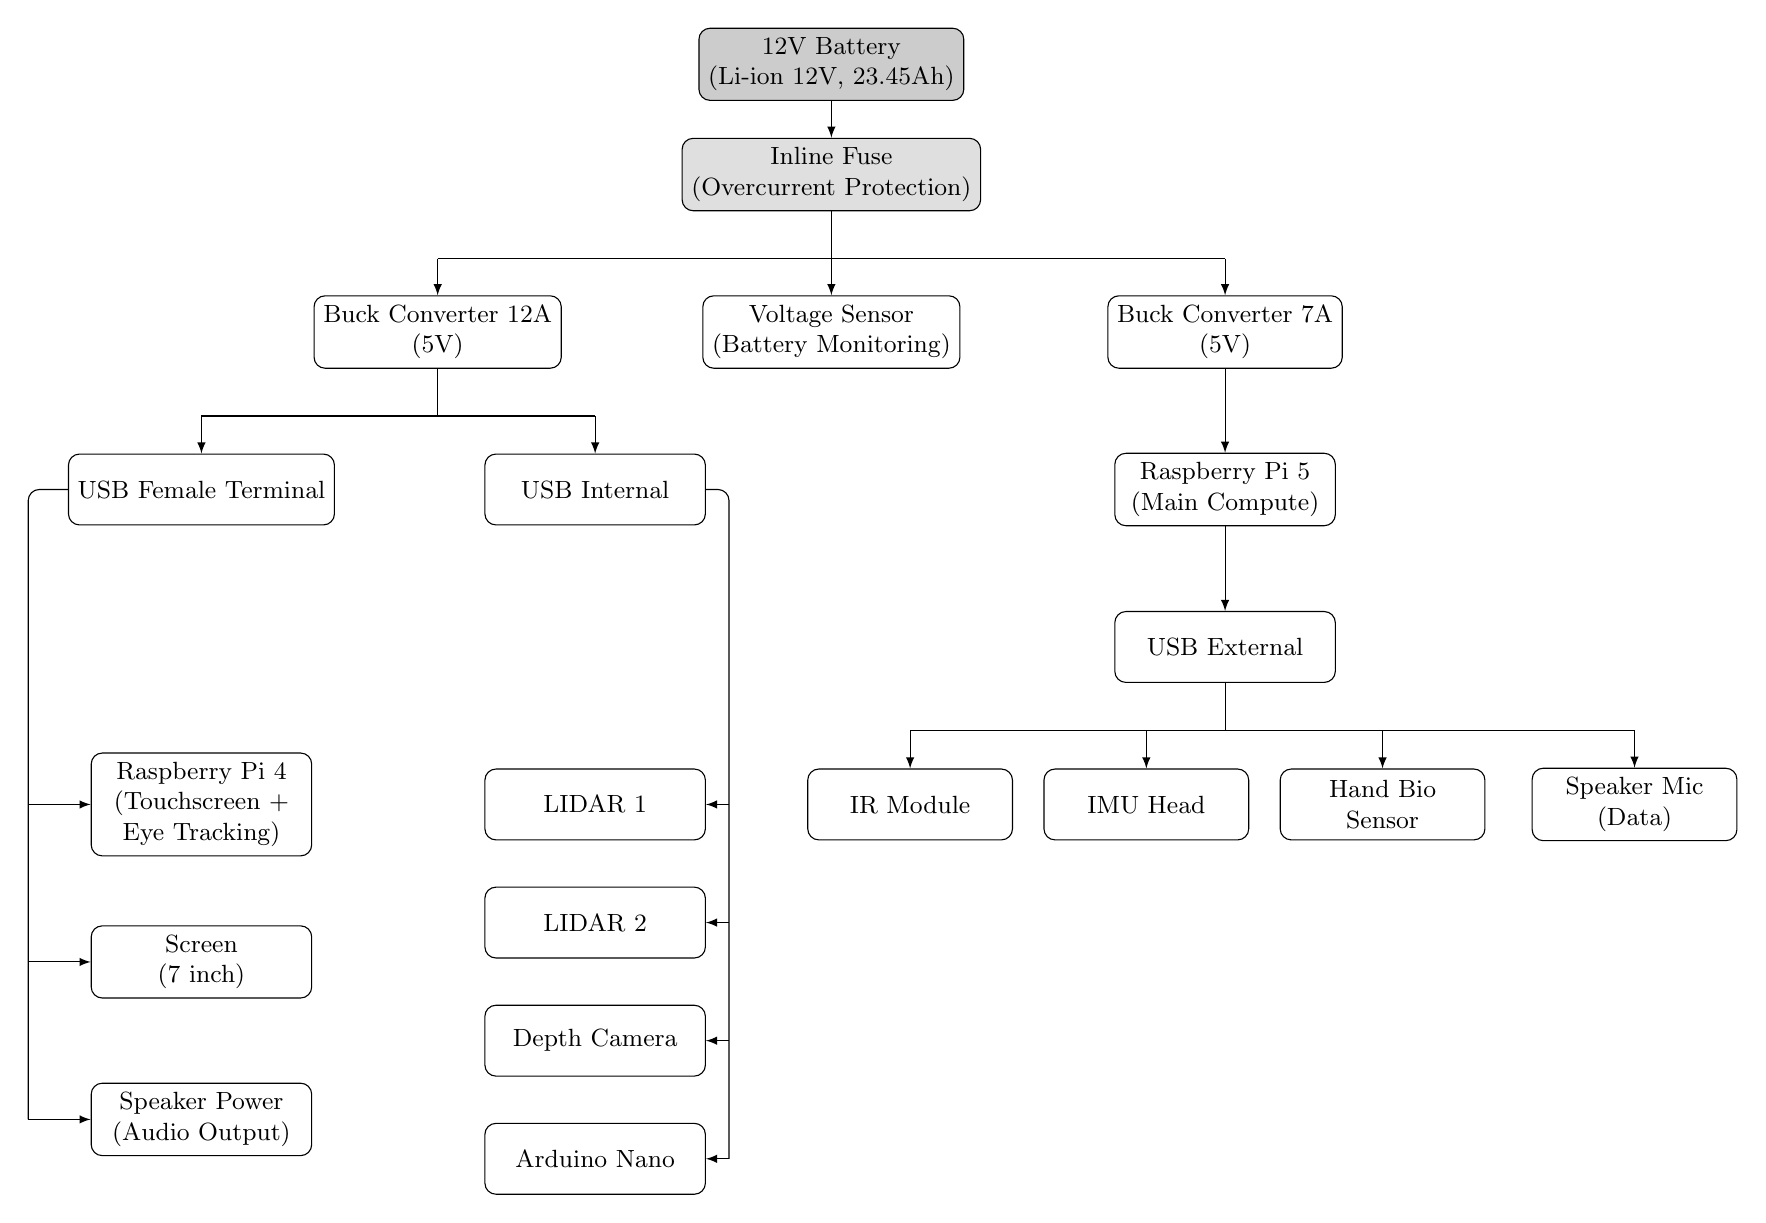
\begin{tikzpicture}[
>=latex,
node distance=1.1cm,
block/.style={
draw,
rounded corners,
minimum width=2.8cm,
minimum height=0.9cm,
align=center,
font=\small
},
bus/.style={
draw,
rounded corners,
minimum width=3.2cm,
minimum height=0.9cm,
align=center,
font=\small
},
every path/.style={rounded corners}
]
%========================
% Top Level
%========================
\node[block,fill=gray!40] (battery)
{12V Battery\\(Li-ion 12V, 23.45Ah)};
\node[block,fill=gray!25] (fuse) at (0,-1.4)
{Inline Fuse\\(Overcurrent Protection)};
\node[block] (buck12) at (-5,-3.4)
{Buck Converter 12A\\(5V)};
\node[block] (sensor) at (0,-3.4)
{Voltage Sensor\\(Battery Monitoring)};
\node[block] (buck7) at (5,-3.4)
{Buck Converter 7A\\(5V)};
% ---- Battery: through the fuse, ONE trunk out, then branch to 3 ----
\draw[->] (battery.south) -- (fuse.north);
\draw (fuse.south) -- ++(0,-0.6) coordinate (battrunk);
\draw (battrunk -| buck12.north) -- (battrunk -| buck7.north);
\draw[->] (battrunk -| buck12.north) -- (buck12.north);
\draw[->] (battrunk)                -- (sensor.north);
\draw[->] (battrunk -| buck7.north) -- (buck7.north);
%========================
% Left Side
%========================
\node[block] (usbf) at (-8,-5.4)
{USB Female Terminal};
\node[block] (usbi) at (-3,-5.4)
{USB Internal};
% ---- buck12: ONE trunk out, then branch to 2 ----
\draw (buck12.south) -- ++(0,-0.6) coordinate (b12trunk);
\draw (b12trunk -| usbf.north) -- (b12trunk -| usbi.north);
\draw[->] (b12trunk -| usbf.north) -- (usbf.north);
\draw[->] (b12trunk -| usbi.north) -- (usbi.north);
% ---- USB Female Terminal: turn 90 right beside block, then straight down till last block ----
\node[block] (rpi4) at (-8,-9.4)
{Raspberry Pi 4\\(Touchscreen +\\Eye Tracking)};
\node[block] (screen) at (-8,-11.4)
{Screen\\(7 inch)};
\node[block] (speaker) at (-8,-13.4)
{Speaker Power\\(Audio Output)};
\draw (usbf.west) -| (-10.2,-13.4);
\draw[->] (-10.2,-9.4)  -- (rpi4.west);
\draw[->] (-10.2,-11.4) -- (screen.west);
\draw[->] (-10.2,-13.4) -- (speaker.west);
% ---- USB Internal: turn 90 right beside block, then straight down till last block ----
\node[block] (lidar1) at (-3,-9.4)
{LIDAR 1};
\node[block] (lidar2) at (-3,-10.9)
{LIDAR 2};
\node[block] (depth) at (-3,-12.4)
{Depth Camera};
\node[block] (nano) at (-3,-13.9)
{Arduino Nano};
\draw (usbi.east) -| (-1.3,-13.9);
\draw[->] (-1.3,-9.4)    -- (lidar1.east);
\draw[->] (-1.3,-10.9)  -- (lidar2.east);
\draw[->] (-1.3,-12.4)   -- (depth.east);
\draw[->] (-1.3,-13.9) -- (nano.east);
%========================
% Right Side
%========================
\node[block] (rpi5) at (5,-5.4)
{Raspberry Pi 5\\(Main Compute)};
\node[block] (usbext) at (5,-7.4)
{USB External};
\draw[->] (buck7.south) -- (rpi5.north);
\draw[->] (rpi5.south) -- (usbext.north);
%========================
% External devices
%========================
\node[
draw,
rounded corners,
minimum width=2.6cm,
minimum height=0.9cm,
font=\small,
align=center
] (ir) at (1,-9.4)
{IR Module};
\node[
draw,
rounded corners,
minimum width=2.6cm,
minimum height=0.9cm,
font=\small,
align=center
] (imu) at (4,-9.4)
{IMU Head};
\node[
draw,
rounded corners,
minimum width=2.6cm,
minimum height=0.9cm,
font=\small,
align=center
] (bio) at (7,-9.4)
{Hand Bio\\Sensor};
\node[
draw,
rounded corners,
minimum width=2.6cm,
minimum height=0.9cm,
font=\small,
align=center
] (mic) at (10.2,-9.4)
{Speaker Mic\\(Data)};
% ---- USB External: ONE trunk out, then branch to 4 ----
\draw (usbext.south) -- ++(0,-0.6) coordinate (uexttrunk);
\draw (uexttrunk -| ir.north) -- (uexttrunk -| mic.north);
\draw[->] (uexttrunk -| ir.north)  -- (ir.north);
\draw[->] (uexttrunk -| imu.north) -- (imu.north);
\draw[->] (uexttrunk -| bio.north) -- (bio.north);
\draw[->] (uexttrunk -| mic.north) -- (mic.north);
\end{tikzpicture}
}
\caption{Power distribution architecture, including the protective inline fuse placed between the battery and the downstream regulation stages.}
\label{fig:power-distribution}
\end{figure}
\subsection{Power Consumption Analysis}
To size the buck converters and estimate battery runtime, the maximum power consumption of each component was tabulated for both 5\,V rails. Table~\ref{tab:power-rpi5-rail} lists the components on the 7~A Raspberry Pi 5 rail, Table~\ref{tab:power-12a} lists the components on the 12~A peripheral rail, and Table~\ref{tab:power-summary} summarizes the totals for both rails.

\begin{table}[H]
\centering
\caption{Raspberry Pi 5 rail power consumption.}
\label{tab:power-rpi5-rail}
\begin{tabular}{l c c c}
\hline
Component & Voltage (V) & Max Current (A) & Power (W) \\
\hline
IMU Head Sensor & 5 & 0.05 & 0.25 \\
IR Module & 5 & 0.03 & 0.15 \\
Hand Bio Sensor & 5 & 0.10 & 0.50 \\
USB Microphone & 5 & 0.10 & 0.50 \\
\hline
Total & -- & 0.28 & 1.40 \\
\hline
\end{tabular}
\end{table}

\begin{table}[H]
\centering
\caption{Buck converter 12\,A (5\,V) rail power consumption.}
\label{tab:power-12a}
\begin{tabular}{l c c c}
\hline
Component & Voltage (V) & Max Current (A) & Power (W) \\
\hline
Raspberry Pi 4 & 5 & 2.5 & 12.5 \\
Screen (7 inch) & 5 & 0.74 & 3.7 \\
Speaker Power & 5 & 1.00 & 5.0 \\
LiDAR (LD06) -- unit 1 & 5 & 0.30 & 1.5 \\
LiDAR (LD06) -- unit 2 & 5 & 0.30 & 1.5 \\
Depth Camera & 5 & 0.50 & 2.5 \\
Arduino Nano & 5 & 0.035 & 0.175 \\
\hline
Total & -- & 5.375 & 26.875 \\
\hline
\end{tabular}
\end{table}

\begin{table}[H]
\centering
\caption{Overall 5\,V rail power summary.}
\label{tab:power-summary}
\begin{tabular}{l c c}
\hline
Rail & Current (A) & Power (W) \\
\hline
Buck Converter 7\,A (5\,V) & 5 & 25 \\
Buck Converter 12\,A (5\,V) & 5.375 & 26.875 \\
\hline
Total & 10.375 & 51.875 \\
\hline
\end{tabular}
\end{table}

As summarized in Table~\ref{tab:power-summary}, the combined current draw on the 12\,V input battery is therefore approximately 10.375\,A, corresponding to a total power consumption of about 51.875\,W across both 5\,V rails. To protect the battery and wiring from fault conditions, an inline fuse rated above this normal operating current (e.g., a 15~A fuse, chosen to sit safely above the 10.375~A steady-state draw while still tripping well below typical wiring and connector current limits) is installed directly at the battery output, ahead of the voltage sensor and both buck converters, as shown in Figure~\ref{fig:power-distribution}.

\subsection*{Battery \& Runtime Estimation}
With the total power consumption established, the usable runtime of the 12\,V compute-and-sensor battery can be estimated from its rated energy capacity.
\[
\text{Battery Energy} = 12\ \text{V} \times 23.45\ \text{Ah} = 281.4\ \text{Wh}
\]
\[
\text{Estimated Runtime} = \frac{281.4\ \text{Wh}}{51.875\ \text{W}} \approx 5.42\ \text{h}
\]
This gives an estimated continuous runtime of approximately 5.4 hours for the compute and sensor subsystem under maximum load, which is independent of the wheelchair's separate 24\,V drive battery.

% ============================================================
\section{Bill of Materials \& Cost Estimation}
% ============================================================

To evaluate the economic feasibility of the Sanad autonomous wheelchair, a detailed Bill of Materials (BOM) has been compiled. One of the core design goals of Sanad was to construct a highly capable, autonomous cyber-physical platform using consumer-grade sensors and open-source software, keeping the total cost at a fraction of commercial smart wheelchairs, which often exceed \$10\,000 to \$20\,000 USD.

The hardware implementation is built upon a standard commercial powered wheelchair, retrofitted with sensors, an onboard host computer, low-level microcontrollers, and custom-designed 3D-printed mounts. Table~\ref{table:bom_cost_estimation} outlines the cost breakdown of the prototype in both Egyptian Pounds (EGP) and US Dollars (USD), based on market prices at the time of development.
\begin{table}[H]
\centering
\caption{Bill of Materials (BOM) and Cost Estimation for the Sanad Prototype.}
\label{table:bom_cost_estimation}
\small
\begin{tabularx}{\textwidth}{|l|X|c|r|r|}
\hline
\textbf{Category} & \textbf{Component Description} & \textbf{Qty} & \textbf{Unit Cost (EGP)} & \textbf{Total Cost (EGP)} \\
\hline
Chassis & Base Foldable Electric Wheelchair (24V, 250W motors) & 1 & 20,000 & 20,000 \\
\hline
Compute & Raspberry Pi 5 (8GB RAM) --- main compute & 1 & 14,000 & 14,000 \\
\hline
\multirow{3}{*}{Perception}
 & LD19 Planar LiDAR Rangefinder & 2 & 4,500 & 9,000 \\
\cline{2-5}
 & Front-Facing RGB-D Depth Camera & 1 & 7,500 & 7,500 \\
\cline{2-5}
 & BNO055 Inertial Measurement Unit (IMU) & 1 & 3,500 & 3,500 \\
\hline
Power & 12V 23.45Ah Battery Pack & 1 & 3,750 & 3,750 \\
\hline
Mechanical & 3D-Printed PETG Mounts, GT2 Pulley-Belt \& Fasteners & 1 & 2,000 & 2,000 \\
\hline
Electronics & Custom Arduino Nano Interface PCB + Dual Buck Converters (7A/12A) + Dual hub & 1 & 1,750 & 1,750 \\
\hline
\multicolumn{3}{|r|}{\textbf{Subtotal --- Base Platform (without Modules)}} & & \textbf{61,500 EGP} \\
\hline
\multirow{2}{*}{Modules}
 & Touchscreen Interface --- 7" LCD + Secondary Raspberry Pi 4 (8GB) & 1 & 3,000 + 9,400 & 12,400 \\
\cline{2-5}
 & Head-Motion Control --- Wearable IMU + ESP32-C3 & 1 & 950 + 250 & 1,200 \\
\hline
\multicolumn{3}{|l|}{\textbf{Total Project Cost (with Modules)}} & & \textbf{75,075 EGP} \\
\hline
\end{tabularx}
\end{table}

This estimation demonstrates that the entire autonomous and multi-modal platform can be assembled for approximately 75,075 EGP, including the touchscreen and head-motion assistive module stack. The base navigation-and-mobility platform alone — chassis, compute, perception, power, and control electronics, without either assistive module — costs approximately 61,500 EGP, meaning the two plug-and-play modules add roughly 13,575 EGP to the total. By leveraging open-source middleware (ROS 2, Nav2, SLAM Toolbox) and custom software logic, Sanad eliminates the prohibitive licensing fees associated with proprietary assistive technology, making autonomous mobility and smart home control accessible to middle- and lower-income families.

\section{Summary and Transition}
This chapter has detailed the physical design, fabrication choices, motor control tuning, and cost estimates of the Sanad wheelchair. The next chapter, Chapter 11 (Conclusion), concludes the book by synthesizing project achievements and outlining future design roadmaps.

\chapterseparator{Chapter 11}
\setcounter{chapter}{11} 
\chapter*{Chapter (11): Conclusion}
\addcontentsline{toc}{chapter}{Chapter (11): Conclusion} 
\setcounter{section}{0}

% ============================================================
\section{Chapter Preview}
This chapter synthesizes the outcomes and contributions of the Sanad project. It highlights the achievements in autonomous navigation, multi-modal interfaces, home/social integration, caregiver remote diagnostics, and details a future development roadmap for the platform.

\section{Conclusion}
% ============================================================

In this graduation project, we designed, developed, and validated \textbf{Sanad}, a fully integrated, autonomous, and multi-modal assistive wheelchair platform. The project successfully addresses a critical gap in assistive technology: the exclusion of individuals with severe physical and cognitive motor impairments (such as quadriplegia, advanced ALS, and visual impairments) from standard manual-control powered wheelchairs.

The technical contributions and findings of the project can be summarized as follows:
\begin{enumerate}
    \item \textbf{Autonomous Navigation:} By transitioning from manual, open-loop control to an autonomous, closed-loop robotic stack using ROS 2, Sanad allows users to navigate indoor environments safely through high-level goals. The system successfully fuses wheel odometry, IMU data, and dual LiDAR scans (providing a full 360-degree obstacle field of view) to localise and plan trajectories with centimeter-level precision.
    \item \textbf{Multi-Modal Accessibility:} Sanad accommodates diverse disability profiles by offering multiple control channels. Voice command parsing utilizing large language models allows natural-language conversational interaction in Egyptian Arabic. For non-verbal or locked-in patients, eye-tracking cursor navigation provides hands-free operation of the system kiosk. The IMU head-gestures module offers intuitive manual adjustment within room interiors.
    \item \textbf{Environmental and Social Integration:} By embedding smart-home control and Telegram messaging directly into the wheelchair platform, the user's independence is expanded beyond locomotion. The system empowers users to control environmental appliances and interact with remote caregivers independently.
    \item \textbf{Caregiver Diagnostics:} The companion mobile application and backend server establish a robust monitoring network, streaming biometric vitals (BPM, $SpO_2$) and wheelchair telemetry to ensure user safety.
\end{enumerate}

Ultimately, Sanad demonstrates that advanced robotics and artificial intelligence can be combined with affordable consumer hardware to build a life-altering assistive device, restoring basic autonomy and dignity to individuals who would otherwise be confined to constant caregiver assistance.

% ============================================================
\section{Future Features \& Roadmap}
% ============================================================

While the current implementation of Sanad has met its core design requirements, several key areas have been identified for future research, development, and commercialization:

\begin{itemize}
    \item \textbf{Multimodal Local Large Language Models:} Currently, the conversational NLP pipeline relies on Google Cloud Vertex AI (Gemini), falling back to a simplified local model during internet outages. Future iterations will optimize lightweight local models (e.g., LLaMA-3-8B quantized) running entirely onboard the host computer via specialized hardware accelerators (like the Intel Arc GPU or NVIDIA Jetson platforms) to ensure offline conversational performance without latency.
    \item \textbf{Advanced Vision-Language Model (VLM) Grounding:} Integrating real-time VLM spatial reasoning will allow users to navigate to unmapped or descriptive locations (e.g., saying ``take me to the red armchair'' or ``park next to the water dispenser''). The onboard camera feed can be analyzed dynamically by the VLM to resolve target coordinates.
    \item \textbf{Brain-Computer Interface (BCI) Control:} For users in the most advanced stages of motor impairment (such as advanced locked-in syndrome), the system can integrate non-invasive EEG-based brain-computer interfaces. By analyzing neural signals (like motor imagery or P300 potentials), the BCI can allow the user to select navigation commands or trigger motion goals, sending commands directly to the core software orchestration and command arbitration layer.
    \item \textbf{Augmented Reality (AR) Glasses Integration:} To improve accessibility and user experience, the physical touchscreen display can be replaced or augmented with lightweight AR glasses. This allows heads-up visualization of the user options. Furthermore, the system can project navigation data onto the user's field of view, displaying a real-time projection of the planned path, the distance to the goal, and the expected time of arrival (ETA).
    \item \textbf{Assistive Robotic Arm Integration:} To address the complete lack of upper-limb function in quadriplegic users, the wheelchair chassis can be retrofitted with a lightweight robotic manipulator arm. This arm will automate daily activities requiring hand interaction, such as opening the refrigerator door, pushing elevator or doorbell buttons, and fetching light objects, executed via high-level voice or gaze-based commands.
    \item \textbf{Active Suspension and Outdoor Trajectory Planning:} The current system is optimized for flat, indoor surfaces. Designing an active mechanical suspension and integrating 3D point cloud mapping (using depth cameras and 3D LiDAR) will enable the wheelchair to traverse uneven outdoor terrain, ramps, and pavements.
    \item \textbf{Dynamic Social Navigation:} Incorporating social navigation planners will allow the wheelchair to predict human motion paths in crowded domestic or public spaces, adjusting its speed and trajectory according to social norms (e.g., maintaining a respectful distance and passing on the appropriate side).
\end{itemize}

\section{Closing Remarks}
By demonstrating a viable end-to-end integration of SLAM navigation, LLM-based Egyptian Arabic voice routing, and eye-gaze tracking on affordable single-board computers, Sanad provides a blueprint for next-generation assistive devices. This prototype establishes that high-level autonomy and multi-modal accessibility can be unified to restore independence and dignity to users with severe motor impairments.


\chapterseparator{Appendix}
\chapter*{Appendix: Project Assets \& Repositories}
\addcontentsline{toc}{chapter}{Appendix: Project Assets \& Repositories}
\setcounter{section}{0}

This appendix provides links to the official software repositories and the central Google Drive directory containing all project assets. These assets include CAD designs, PCB electrical schematics, user testing videos, and presentation slides.

\section*{Software Repositories}

The Sanad wheelchair platform is modularly designed across several software repositories. All codebases are open-source and hosted on GitHub under the \textbf{Sanad Chair} organization. 

To access all repositories, including the core ROS 2 workspace, backend server, mobile application, kiosk interface, and documentation, visit:
\begin{center}
    \url{https://github.com/sanadChair}
\end{center}

\section*{Project Assets \& Google Drive}

All physical design assets, including the SolidWorks CAD assembly of the wheelchair chassis, custom PCB wiring layouts, user testing videos, and presentation slides, are stored in a shared Google Drive directory. 

Scan the QR code in Figure~\ref{fig:drive_qr_code} or use the URL below to access the drive directory:
\begin{center}
    \url{https://drive.google.com/drive/folders/1UTUv9_mNRz85AxI-6V7NWe3aIXW6B8WS?usp=sharing}
\end{center}

\begin{figure}[H]
    \centering
    
\includegraphics[width=0.4\linewidth]{figures/appendix/drive_qr.png}
    \caption{QR Code to access the project Google Drive (contains CAD models, PCBs, slides, and media).}
    \label{fig:drive_qr_code}
\end{figure}

\nocite{*}
% \vspace*{-1.5cm}
\bibliographystyle{plain}
\bibliography{references}
\newpage


\end{document}